\documentclass[a4paper,12pt,twoside]{book}

% Encodage des caractères et langue du document
\usepackage[T1]{fontenc}
\usepackage[utf8]{inputenc}
\usepackage{lmodern}
\usepackage[french]{babel}
\usepackage{amsfonts}
\usepackage{bm}
\usepackage{graphicx}
\usepackage{float}
\usepackage{dcolumn}
\usepackage{multicol}
\usepackage[font={small}]{caption}
\usepackage{subcaption}
\usepackage{placeins}
\usepackage{appendix}

\setcounter{tocdepth}{2} % Pour que les subsubsections n'apparaissent pas dans la TOC
\setcounter{secnumdepth}{2} % Pour que les subsubsections ne soient pas numérotées

% Gestions des marges
\usepackage{geometry} 
\geometry{a4paper}
%\geometry{margin=2.5cm}
%\geometry{headheight=6mm}

% Si on a besoin d'une configuration plus précise des marges
\geometry{%
  a4paper,                % format de papier
% Définition des marges :
  left= 3cm,            % marge intérieure à la page
  right = 2cm,          % marge extérieure
  top = 3cm,
  bottom = 3cm,
% En-tête et pied de page :
  headheight=6mm,         % espace réservé à l'en-tête dans la marge top
  %headsep=3mm,            % espace entre le corps et l'en-tête
  %footskip=9mm            % espace entre le corps et le pied de page
}

% Pour une meilleure gestion des maths
\usepackage{amsmath,amssymb,amsfonts,amsthm}
%\usepackage{mathtools} % version modifiée de amsmath, ajoute des symboles, etc.
\usepackage{mathrsfs}% pour rajouter un format de lettres façon "caligraphie" en math mode.

% Pour gérer les unités
\usepackage{siunitx}
\sisetup{inter-unit-product=\ensuremath{{}\cdot{}}} % pour mettre des points médians entre les unités quand il y en a plusieurs
\sisetup{separate-uncertainty=true,multi-part-units=single} % pour faire des incertitudes en écrivant \SI{valeur(incertitude)}{unité}
\DeclareSIUnit\vitesse{\meter\per\second}


% Pour une meilleure gestion des graphiques
\usepackage{graphicx}
\usepackage[export]{adjustbox}
\usepackage{caption}
\usepackage{subcaption} % permet de faire des subfigures (remplace le package subfig)

% Pour les tableaux, matrices, listes
\usepackage{booktabs}
\usepackage{array}
\newcolumntype{P}[1]{>{\centering\arraybackslash}p{#1}}
\usepackage{paralist} % si besoin regarder "enumitem" qui est un peu différent
%\usepackage{multirow} % pour faire des tableaux plus compliqués
\usepackage{esint}

% Pour personnaliser les entêtes et pieds de pages
\usepackage{fancyhdr}
\usepackage{emptypage} % garantit que les pages blanches avant les débuts de chapitres soient vraiment blanches (pas d'entête ni de pied de page)
 
 % On définit le style pour les pages "normales"
\pagestyle{fancy}
\renewcommand{\chaptermark}[1]{\markboth{\chaptername \ \thechapter.\ #1}{}} % sert à personnaliser l'affichage de \leftmark (ici : le mot "Chapitre", le numéro, un point, et le titre du chapitre, sans écrire en majuscules)
\renewcommand{\sectionmark}[1]{\markright{\thesection.\ #1}} % sert à personnaliser l'affichage de \rightmark (ici : le numéro et le titre de la section en cours, sans écrire en majuscules)
\fancyhf{} % assure que les entête et pieds de page sont vides au départ
\fancyhead[LE]{\leftmark}
\fancyhead[RO]{\rightmark}
\fancyfoot[LE,RO]{\thepage}

% On définit le style pour les pages "spéciales" (début de chapitre, table des matières, etc.)
\fancypagestyle{plain}{
\fancyhf{}
\fancyfoot[RO,RE]{\thepage}
\renewcommand{\headrulewidth}{0pt}
\renewcommand{\footrulewidth}{0pt}}

% Explications :
% L = left, R = right, C = center, E = even pages, O = odd pages
%\thepage : adds number of the current page.
%\thechapter : adds number of the current chapter.
%\thesection : adds number of the current section.
%\chaptername : adds the word "Chapter" in English or its equivalent in the current language.
%\leftmark : adds name and number of the current top-level structure (for example, Chapter for reports and books classes; Section for articles ) in uppercase letters.
%\rightmark : adds name and number of the current next to top-level structure (Section for reports and books; Subsection for articles) in uppercase letters.

% Pour personnaliser les premières pages des chapitres
\usepackage[Lenny]{fncychap}

% Pour la table des matières
\usepackage[nottoc]{tocbibind} % pour que la bibliographie apparaisse dans la table des matières (avec l'option pour que la table des matières elle-même n'apparaisse pas dans la table des matières).
\usepackage{tocloft}% pour pouvoir modifier les tailles d'espacement dans la table des matières
%\setlength\cftaftertoctitleskip{10pt} % pour fixer la taille après le titre "table des matières" et la table des matières en elle-même.

% Divers
\usepackage{textcomp} % rajoute des symboles (notes de musiques, etc.)
\usepackage{xcolor} % pour ajouter de la couleur (si besoin)
\usepackage{epigraph} % pour rajouter des citations en début de chapitre
% Exemple :
%\epigraph{Citation}}{Auteur}
\usepackage{cite} % pour faire citations de façon pratique (notamment mettre [1-3] au lieu de [1,2,3]).
%\usepackage{quotchap} % pour rajouter des citations en début de chapitre (change la présentation des chapitres)
% Exemple :
%\begin{savequote}
%Citation
%\qauthor{Auteur}
%\end{savequote}

% Pour gérer les liens dans le document et avoir les signets dans le PDF
\usepackage{hyperref}
\usepackage{bookmark}
\usepackage{pdfpages}

\newcommand{\todo}[1]{\textcolor{red}{TODO : #1}}
\newcommand{\rem}[1]{\textcolor{blue}{Remarque : #1}}
\newcommand{\act}[1]{\textcolor{green}{Point actuel : #1}}
% Configuration de hyperref
\definecolor{linkcolor}{rgb}{0,0,0.6} % couleur des liens (bleu foncé)
\hypersetup{
	colorlinks=true, % colore les liens au lieu de les encadrer
	pdfstartview=FitV, % ouvre le PDF de façon à ce qu'il prenne la taille verticale de l'écran
	urlcolor=linkcolor, % choix de la couleur des liens URL
	linkcolor= linkcolor, % choix de la couleur des liens internes (table des matières, etc.)
	citecolor=linkcolor % choix de la couleur des liens de citations
}

\providecommand{\annexename}{Annexe}
\newcommand{\annexeref}[1]{\annexename~\nameref{#1}}

\usepackage{titlesec}

\setcounter{secnumdepth}{3}

\titleformat{\paragraph}
{\normalfont\normalsize\bfseries}{\theparagraph}{1em}{}
\titlespacing*{\paragraph}
{0pt}{3.25ex plus 1ex minus .2ex}{1.5ex plus .2ex}

\title{Template de thèse minimaliste}
\author{Antoine Bérut}
\date\today

\begin{document}

\frontmatter

%\maketitle
\thispagestyle{empty}

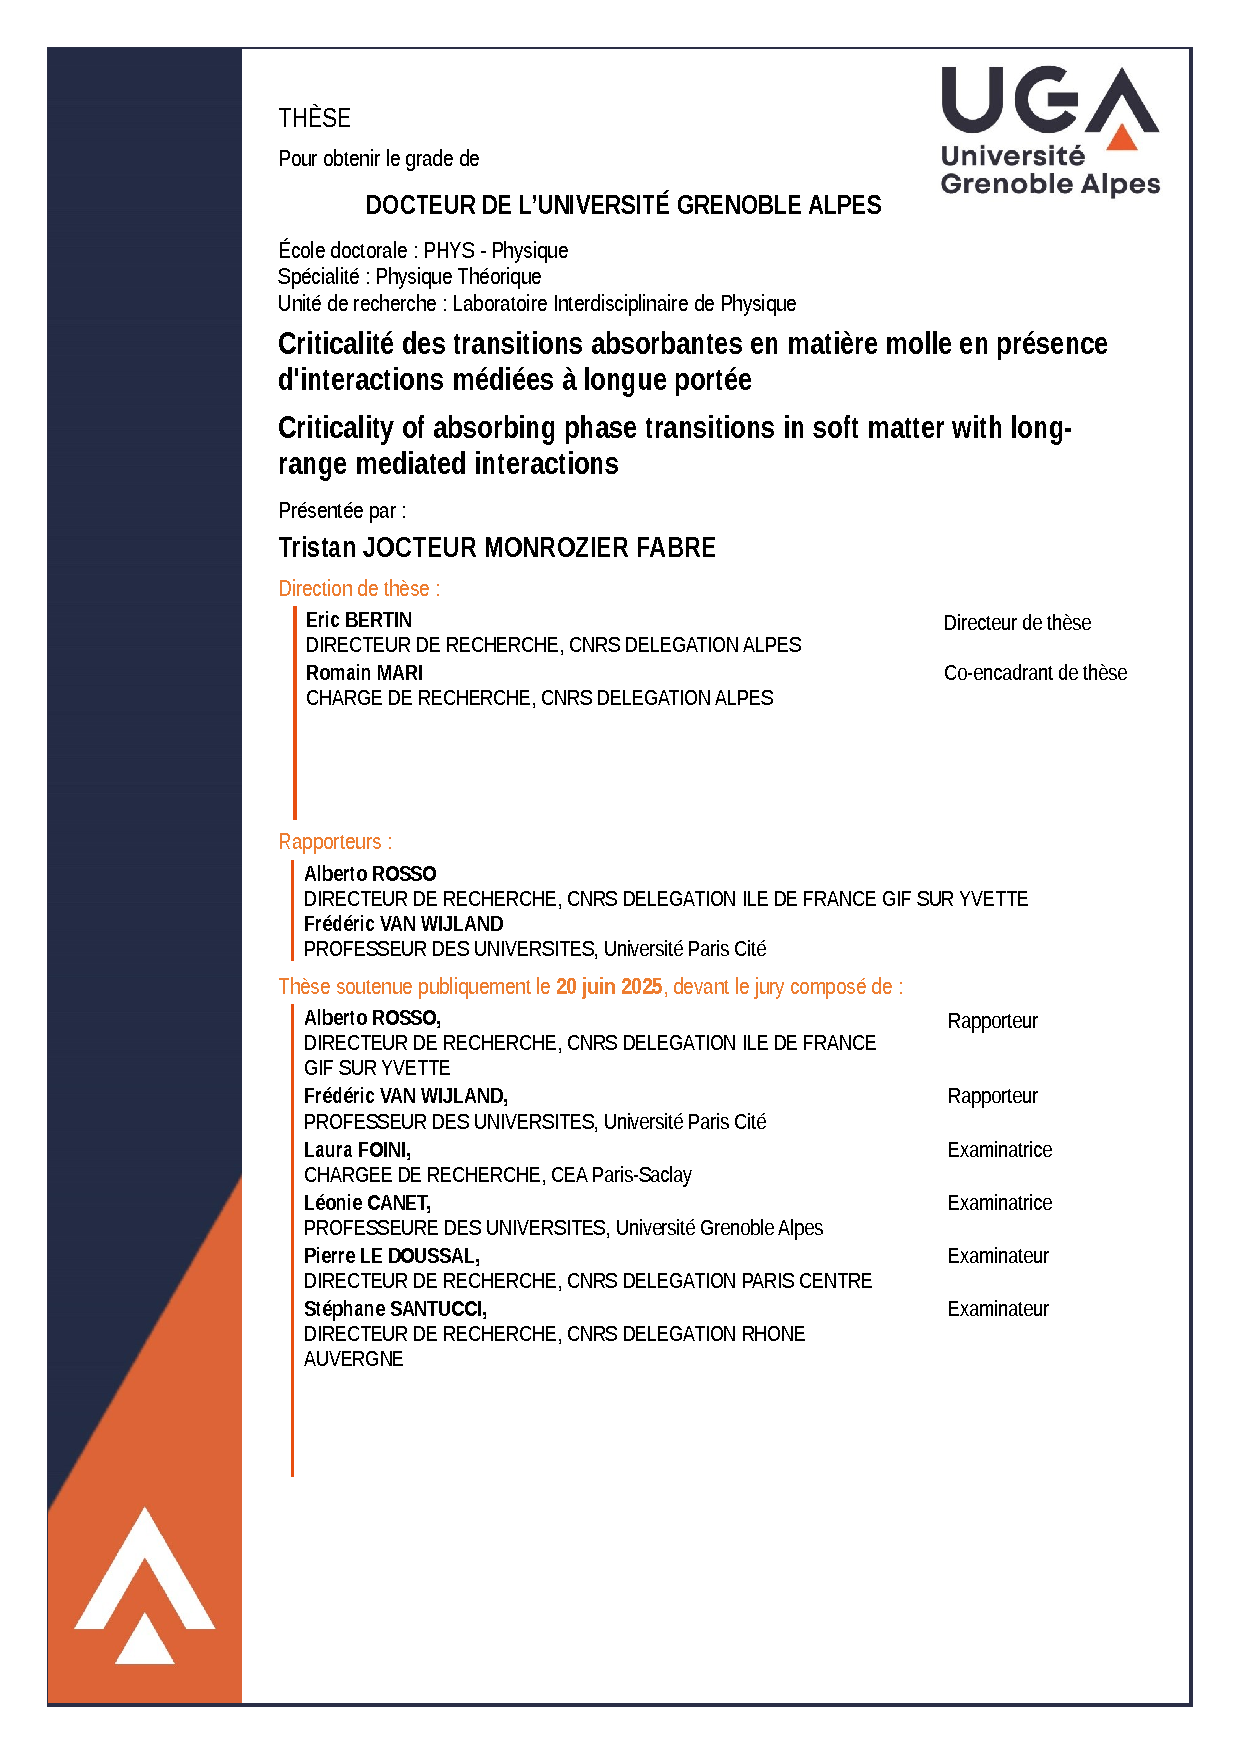
\includepdf[noautoscale=true, width=\paperwidth]{couverture_these.pdf}


\newpage

\thispagestyle{empty}
\newpage\phantom{blabla}
\newpage
\thispagestyle{empty}

\begin{small}
\tableofcontents
\end{small}

\mainmatter
\thispagestyle{empty}

\section*{Remerciements}

\subparagraph{}Je tiens tout d'abord à remercier Eric et Romain, mes deux encadrants durant ces trois années de thèse. Si j'ai pu mener à bien ces recherches c'est grâce à leur expertise mais aussi et surtout grâce à la bienveillance dans leur encadrement. Ils ont su se rendre disponible pour m'aider lorsque j'en avais besoin, m'ont fait confiance en me donnant une grande liberté et m'ont écouté quand les choses allaient moins bien pour moi. Je pense que c'est avant-tout les qualités humaines qui font d'un-e chercheureuse un-e bon-ne encadrant-e et j'ai eu énormément de chance de tomber sur vous.

\subparagraph{}Je remercie également Alberto Rosso et Frédéric Van Wijland pour avoir accepté d'être rapporteurs de ce manuscrit et pour leurs retours bienveillants. Aussi, je remercie grandement Léonie Canet, Laura Foini, Pierre Le Doussal et Stéphane Santucci pour avoir accepté de faire partie de mon jury, et pour le plaisir que j'ai pris à échanger avec elleux.

\subparagraph{}J'aimerais remercier aussi les gens avec qui j'ai pu collaborer, notamment Kirsten Martens, Kay Wiese et Cesare Nardini, qui m'ont grandement guidé dans les différents projets.

\subparagraph{}Je remercie par ailleurs plus globalement le LIPhy et tous les gens qui y travaillent. Le personnel administratif, technique mais aussi les agent-es d'entretien qui permettent de rendre ce lieu agréable au quotidien. Aussi, bien sûr, je remercie tous les non-permanents avec qui j'ai pu me sentir à l'aise et partager de nombreux moments, scientifiques ou non, et celleux qui sont devenu-es des ami-es : Cécile, Andréa, Mathieu, Bruno, Marküs, ... Un merci tout particulier à Julia avec qui j'ai partagé mon bureau pendant la moitié du temps et qui m'a presque donné envie de venir au travail. Rien que pour cette rencontre, je ne regrette pas les trois ans de thèse.

\subparagraph{}J'aimerais aussi remercier les gens qui n'étaient pas avec moi au laboratoire mais qui, indirectement, m'ont beaucoup aidé quotidiennement. D'abord Zoë avec qui j'ai toujours pu parler de mes doutes, de mes peurs, m'incruster pour dessiner, partir à la montagne, ... Dans ce genre de situations où souvent rien ne marche comme on veut, c'est toujours bien d'avoir un repère auquel on est sûr de pouvoir se rattacher.

Bien sûr merci aussi à Delphine pour ces trois années à se plaindre de la thèse ensemble, à défaut d'avoir trouvé une stratégie pour abolir le travail. Si cette période était tellement chouette que Steve pourrait la miner, c'était surtout grâce à la petite vie de coloc qu'on a réussi à se construire ensemble. Merci pour le chantage affectif, les soirées complètement random, t'inquiéter quand ça va pas, et me faire rire tout le temps. Malheureusement on n'est plus "là pour 3 ans", et pour ça je crois que ça me rend un peu triste que ça se finisse... mais bref, pas envie d'en parler.

\subparagraph{}Enfin j'aimerais remercier toustes celleux que j'ai moins eu l'occasion de voir mais qui m'ont aidé, à leur manière, pendant ces trois années. Merci à Julie et Julia pour leur soutien, leur amitié, et les week-ends au bord de l'eau. Merci à ma mamie pour les parties de dés entre deux pages de rédaction, au tiroir à cringe pour les distractions quotidiennes, à mes ami-es trentenaires du club de lecture, à ma fanbase Instagram (yu.gui.lot, philosauvage, ...), et beaucoup d'autres...

\thispagestyle{empty}
\newpage
\thispagestyle{empty}

\section*{Résumé}

\small

\subparagraph{}Des fractures solides aux écoulements des milieux granulaires, en passant par le déplacement des interfaces liquides en milieu poreux, de nombreux phénomènes hors d’équilibre en matière molle peuvent être interprétés comme des transitions de phase absorbantes. Celles-ci séparent une phase active, dans laquelle la dynamique du système persiste à temps long, d'une phase absorbante dans laquelle la dynamique se retrouve bloquée au bout d’un temps fini. Les régions où la dynamique prend place sont considérées comme actives, comme dans le cas des zones plastiques lors de l'écoulement des matériaux amorphes. Il en résulte un champ d’activité (à ne pas confondre avec la notion d’activité en matière active, qui renvoie à des forces hors d’équilibre) dont la dynamique permet de caractériser la transition de phase absorbante considérée, donnant lieu à un comportement critique spatio-temporel.

\subparagraph{}De la même manière qu'à l'équilibre, cette caractérisation en tant que phénomènes critiques met en évidence des comportements communs représentés par des classes d'universalité. Dans ce cas, l'influence des interactions à longue portée sur le comportement critique est comprise dans un cadre théorique clair lorsque celles-ci correspondent à un transport à longue portée. Toutefois, dans le cas d'interactions médiées par le milieu (par exemple le fluide dans lequel des particules sont immergées), dont la longue portée émerge des lois de conservation sous-jacentes, le transport à longue portée peut se voir remplacé par une propagation à longue portée d’un signal, par exemple un bruit mécanique. L'impact de la longue portée sur la criticalité de la transition de phase absorbante peut alors s'avérer surprenant, s'extrayant du cadre de compréhension générique associé au transport à longue portée. C'est notamment le cas pour la transition de réversibilité dans les suspensions cisaillées cycliquement, et pour la transition vers l'écoulement des fluides à seuil. \`A travers l'étude spécifique de ces deux transitions initialement proches de la classe de la percolation dirigée conservée, ce travail numérique et théorique vise à mieux comprendre l'impact de ce type d'interactions à longue portée sur le comportement critique.

\subparagraph{}Dans une première partie, nous caractérisons quantitativement le cadre générique du transport à longue portée en deux dimensions, correspondant à un transport de particules à longue portée. Par l'étude généralisée de modèles emblématiques de la percolation dirigée conservée, nous déterminons les exposants critiques statiques, dynamiques et d'hyperuniformité associés et leurs évolutions avec la portée. Cette étude sert alors de base de comparaison pour l'analyse des transitions sur lesquelles se concentre notre intérêt.

\subparagraph{}Dans une seconde partie, nous caractérisons la transition de réversibilité dans les suspensions et la transition vers l’écoulement des fluides à seuil, qui font toutes deux intervenir des interactions médiées à longue portée.  Par une modélisation numérique simple, nous montrons que celles-ci peuvent exhiber un comportement singulier, montrant une évolution convexe du paramètre d'ordre et des fluctuations qui s'annulent à l'approche du point critique. L'analyse d'autres propriétés, comme l'hyperuniformité à la transition et la dynamique d'avalanches proche du point critique, montre que ce comportement et son évolution avec la portée marquent une claire différence avec le cadre générique associé au transport à longue portée. 

\subparagraph{}Nous proposons finalement un parallèle entre ces deux transitions au comportement critique inhabituel. Notamment, nous établissons un cadre de description commun en champ moyen permettant d'appréhender leurs spécificités en dimension finie. Cette démarche ouvre alors la voie à une compréhension plus générale des transitions de phase absorbantes en présence d'interactions médiées à longue portée assimilables à un bruit interne, dont nous discutons les difficultés.

\vfill

\thispagestyle{empty}

\section*{Abstract}

\subparagraph{}From crack front propagation to the flow of granular materials, through moving liquid interfaces in porous materials, many soft matter out-of-equilibrium phenomena can be considered as absorbing phase transitions. These transitions separate an active phase, in which the dynamics continues indefinitely, from an absorbing phase, in which the dynamics become trapped at a finite time. Regions where these dynamics occur are considered active, similar to plastic regions in the flow of amorphous materials. This defines an activity field (not to be confused with activity in active matter, which stems from out-of-equilibrium forces), whose dynamics characterize the associated absorbing phase transition, giving rise to a spatiotemporal critical behavior.

\subparagraph{}As in equilibrium systems, these critical behaviors are gathered into universality classes. In this context, the influence of long-range interactions on criticality is well understood within a clear theoretical framework when they are associated with long-range transport. However, in the case of mediated interactions through the embedding medium (e.g. the fluid in which particles evolve), whose long-range character naturally emerges from underlying conservation laws, the long-range transport is replaced by the long-range propagation of a signal, such as mechanical noise. The impact of the range of interaction on the transition's criticality can, in this case, be unexpectedly different, marking a clear difference with the canonical framework associated with long-range transport. This is observed in the reversible-irreversible transition of cyclically sheared suspensions and in the yielding transition of amorphous materials. In this work, we study these two transitions, initially close to the conserved directed percolation class, to better understand the role of this kind of long-range interactions in the critical behavior.

\subparagraph{}First, we quantitatively characterize the canonical framework in two dimensions, corresponding to the long-range transport of particles. By studying emblematic models of the conserved directed percolation class, we determine the associated critical static, dynamic, and hyperuniform exponents and their evolution with the range of transport. This serves as a basis for comparison with the transitions of interest that we focus on in the following sections.

\subparagraph{}Second, we characterize the reversible-irreversible transition in suspensions and the yielding transition, both involving long-range mediated interactions. Using simple numerical models, we show that these transitions can exhibit singular behavior, with a convex evolution of the order parameter and vanishing fluctuations as the critical point is approached. The study of other properties, such as hyperuniformity and avalanche dynamics, reveals that this critical behavior and its evolution with the range of interaction show strong differences with the canonical framework associated with long-range transport.

\subparagraph{}Finally, we draw a parallel between these two unusual transitions. In particular, we propose a mean-field framework capable of capturing their specificities in finite dimensions. This paves the way for a broader understanding of absorbing phase transitions in the presence of mediated long-range interactions, for which we also discuss the challenges.

\thispagestyle{empty}

\chapter{Criticalité absorbante et interactions à longue portée en matière molle}

\label{chapter:introduction}

\subparagraph{}Dans cette thèse, nous présentons l'étude comparée de deux phénomènes de matière molle : la transition de réversibilité dans les suspensions cisaillées cycliquement et la transition vers l'écoulement des fluides à seuil. Le but de ce chapitre est d'introduire ces deux phénomènes que rien ne rassemble au premier regard et de motiver leur étude comparée comme des transitions de phase absorbantes.

\subparagraph{}Pour ce faire, nous commencerons par présenter succinctement la phénoménologie de ces transitions, mettant en évidence un comportement singulier et des mécanismes communs. Cette première familiarisation nous amènera alors naturellement à un cadre commun pour l'étude de ces deux phénomènes : celui des transitions de phase absorbantes. Nous proposerons alors de prendre un peu de recul en présentant la phénoménologie globale de ces transitions, analogue à celle des phénomènes critiques d'équilibre. Après une description complète de la classe d'universalité de la percolation dirigée conservée, nous montrerons en quoi la transition de réversibilité et la transition vers l'écoulement en représentent des bons candidats. En accord avec les études précédentes de ces deux systèmes, nous montrerons que leur comportement critique s'éloigne fortement de ce cadre théorique et en proposerons une explication via la nature fondamentalement différente des interactions à longue portée présentes dans ces systèmes. Enfin, nous formulerons les problématiques relatives à ce comportement singulier qui guideront notre étude tout au long de cet ouvrage.

\section{Écoulement des fluides à seuil et cisaillement cyclique des suspensions}

\subparagraph{}Dans cette section, nous présentons succinctement et successivement la transition de réversibilité dans les suspensions cisaillées cycliquement et la transition vers l'écoulement des fluides à seuil. Le rapprochement des deux phénoménologies associées nous permettra alors de comprendre en quoi l'étude comparée de ces deux systèmes représente un objet riche et intéressant.

\subsection{Transition de réversibilité dans les suspensions cisaillées cycliquement}

\subparagraph{}Certains systèmes en matière molle présentent un phénomène intriguant sous l'action d'un cisaillement cyclique. Sous une amplitude de déformation relativement faible, ceux-ci finissent par opérer une dynamique réversible à temps long, laissant le système inchangé d'un cycle de déformation à l'autre. Toutefois, si cette amplitude devient suffisamment grande, le système est soumis à des changements irréversibles en permanence, menant à une évolution constante de sa structure au fil des cycles \cite{Eckstein_Bailey_Shapiro_1977, breedveld_shear_induced_2001, drazer_microstructure_2004}. Nous appellerons transition de réversibilité le passage d'une phase à l'autre de ce système.

\begin{figure}[h]
	\centering
	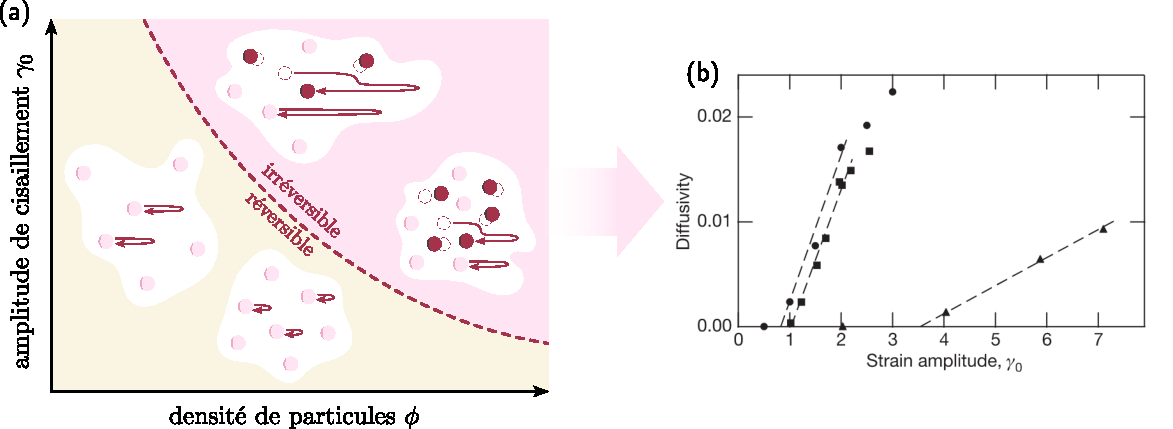
\includegraphics[width=\textwidth]{Chapitre1/Figures/Chapo/suspensions.pdf}
	\caption{(a) Diagramme de phase de la transition de réversibilité inspiré de \cite{maegochi_critical_2021}. Les particules rouges montrent une dynamique irréversible. (b) Évolution du coefficient de diffusion stroboscopique en fonction de l'amplitude de cisaillement dans les expériences de Pine et al. \cite{pine_chaos_2005}}
	\label{fig:suspchapo}
\end{figure}

\subparagraph{}La transition de réversibilité peut être illustrée parfaitement par les expériences menées par Pine et al. \cite{pine_chaos_2005}, dans lesquelles une suspension peu dense est cisaillée dans un écoulement de Couette cylindrique. En suivant l'évolution de la position des particules du système d'un cycle à l'autre, les auteurs ont pu observer deux comportements distincts. Pour une amplitude de cisaillement suffisamment faible $\gamma_0 < \gamma_{0,c}$, les particules conservent la même position d'un cycle à l'autre. Cependant pour $\gamma_0 > \gamma_{0,c}$, les particules se déplacent entre le début et la fin d'un cycle. En étudiant la dynamique stroboscopique du système, i.e. à chaque début de cycle, la suspension est donc immobile pour $\gamma_0 < \gamma_{0,c}$ et elle diffuse pour $\gamma_0 > \gamma_{0,c}$. Il est alors possible de visualiser cette transition en représentant l'évolution du coefficient de diffusion stroboscopique $D_0$ associé en fonction de l'amplitude de cisaillement $\gamma_0$, comme sur la \autoref{fig:suspchapo}-(b).

\subparagraph{}L'origine de cette diffusion stroboscopique à l'échelle macroscopique est attribuée à des interactions microscopiques irréversibles entre les particules, comme illustré sur la \autoref{fig:suspchapo}-(a). Lorsque les particules sont suffisamment éloignées au cours du cisaillement, leur dynamique est uniquement régie par les équations de Stokes, qui ont la propriété d'être réversibles dans le temps. D'un cycle à l'autre, la dynamique est donc identique. Toutefois, lorsque celles-ci sont suffisamment rapprochées par le cisaillement (ou proches initialement du fait d'une forte densité), elles interagissent entre elles au cours du cycle via des interactions locales irréversibles (contacts), induisant de ce fait une évolution d'un cycle à l'autre. C'est la succession de ces interactions irréversibles qui induit une diffusion stroboscopique sous grande amplitude de cisaillement \cite{corte_random_2008}.

\subsection{Transition vers l'écoulement des fluides à seuil}

\subparagraph{}Le second phénomène auquel nous nous intéressons est l'écoulement des fluides à seuil. Les fluides à seuil représentent des objets peuplant notre quotidien à différentes échelles. Nous les retrouvons à l'état naturel par l'écume marine ou les argiles mais aussi par les matériaux d'origine anthropique comme le dentifrice ou la mayonnaise. Leur particularité vient de leurs propriétés rhéologiques, bien plus complexes que celles des fluides newtoniens comme l'eau ou le miel.

\begin{figure}[h]
	\centering
	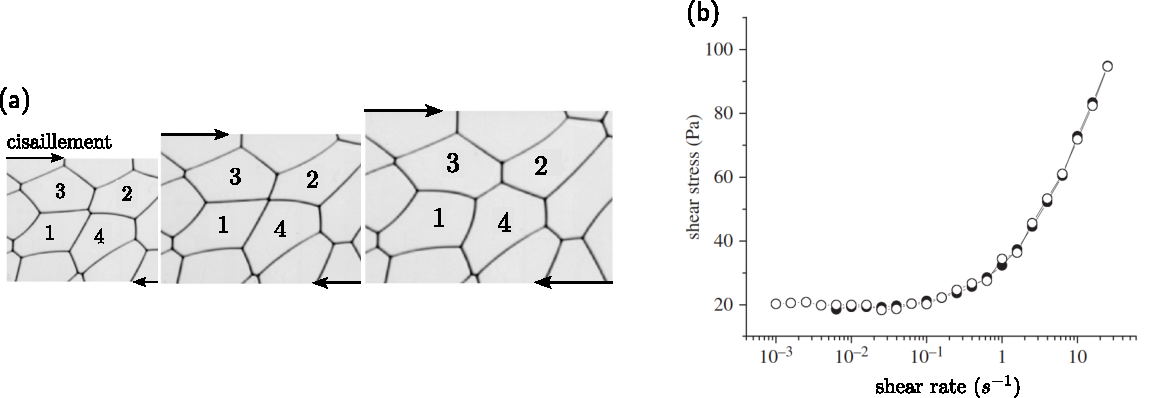
\includegraphics[width=\textwidth]{Chapitre1/Figures/Chapo/yielding.pdf}
	\caption{(a) Image tirée de \cite{dollet_rheology_2014} d'un réarrangement plastique dans une mousse : les bulles voisines changent leur contact afin de minimiser la contrainte supportée. (b) Evolution de la contrainte de cisaillement en fonction du taux de cisaillement appliqué. Données tirées de \cite{moller_origin_2009}}
	\label{fig:yieldingchapo}
\end{figure}


\subparagraph{}Si l'on considère le cas du cisaillement simple  d'un tel fluide, celui-ci possède la spécificité de ne s'écouler que si la contrainte de cisaillement $\Sigma$ appliquée est supérieure à une certaine contrainte seuil $\Sigma_c$ propre au matériau \cite{bonn_yield_2017, nicolas_deformation_2018}. Un exemple édifiant est celui du dentifrice, qui ne s'écoule de son tube que lorsqu'on le presse suffisamment. 

\subparagraph{}En-deçà de la contrainte seuil, après un éventuel régime transitoire, le matériau répond élastiquement à la sollicitation à l'échelle locale comme globale, définissant un taux de cisaillement nul $\dot{\gamma}=0$ dans l'état stationnaire. En revanche, au-delà de cette contrainte seuil, l'état stationnaire du système est caractérisé par la présence continue de réarrangements plastiques locaux (voir \autoref{fig:yieldingchapo}-(a)) \cite{princen_rheology_1986, biance_topological_2009,picard_elastic_2004}. Pour $\Sigma > \Sigma_c$ la succession de ces évènements résulte alors en un écoulement global et donc un taux de cisaillement moyen non-nul $\dot{\gamma}>0$. Il est ainsi possible de visualiser cette transition en représentant l'évolution du taux de cisaillement moyen en fonction de la contrainte appliquée, comme sur l'exemple de la \autoref{fig:yieldingchapo}-(b).


\subsection{Des similarités non-conventionnelles}

\subparagraph{}Ces phénomènes ont en première apparence très peu de points communs. Toutefois, il existe entre eux des similitudes très fortes, illustrées sur la \autoref{fig:banger}. Tout d'abord, comme lae lecteurice l'aura peut-être déjà remarqué, ceux-ci séparent dans chacun des systèmes concernés deux états : un état actif et un état arrêté. Dans le cas de la transition vers l'écoulement l'état actif correspond à un état fluide tandis que dans la transition de réversibilité il correspond à un état diffusant. Par ailleurs, dans les deux cas, ces états actifs sont composés d'une succession d'évènements locaux. Dans le cas de la transition vers l'écoulement ceux-ci sont représentés par les réarrangements plastiques alors que dans le cas de la transition de réversibilité ce sont les interactions de contact irréversibles.

\begin{figure}[H]
	\centering
	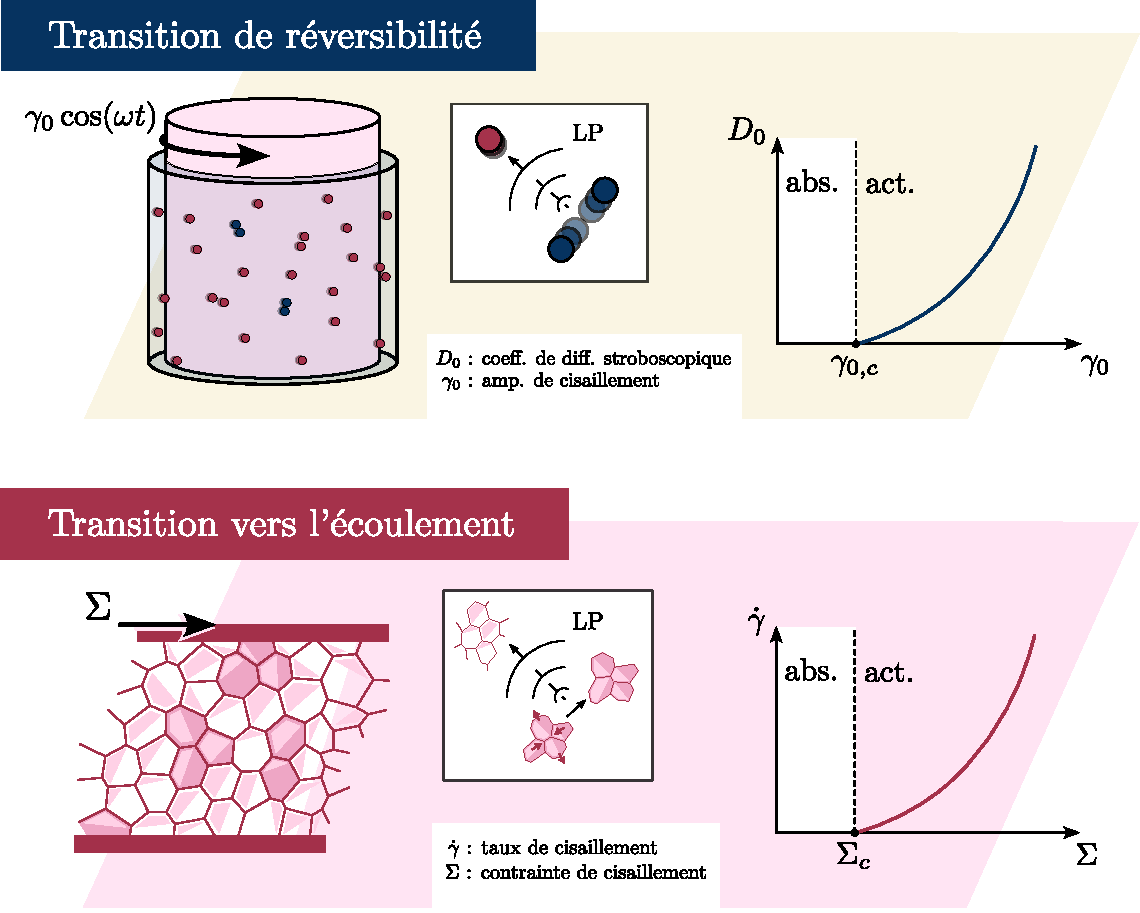
\includegraphics[width=\textwidth]{Chapitre1/Figures/Chapo/Resume.pdf}
	\caption{Illustration schématique du parallèle existant entre la transition de réversibilité dans les suspensions cisaillées cycliquement et la transition vers l'écoulement des matériaux amorphes. LP signifie \textit{longue portée}, abs. signifie \textit{absorbant} et act. signifie \textit{actif}.}
	\label{fig:banger}
\end{figure}

\subparagraph{}De plus, un autre point commun que l'on mettra en évidence dans la suite de ce chapitre est la présence de longue portée. En effet, si dans chacun de ces systèmes la phase active est représentée par des mouvements locaux, il y a de fortes raisons de penser que ceux-ci affectent la dynamique globale via des interactions à longue portée. Dans le cas de la transition de réversibilité dans les suspensions, les particules sont immergées dans un fluide visqueux. Celui-ci est alors capable de propager l'irréversibilité locale à grande distance selon les lois de l'hydrodynamique, affectant de ce fait la dynamique des particules n'interagissant pas directement avec les autres. Dans le cas de la transition vers l'écoulement, les réarrangements plastiques se font dans une matrice élastique. Cette situation largement étudiée montre que ces évènements locaux induisent des interactions à longue portée dans le matériau, susceptibles d'induire d'autres évènements à grande distance. Dans cette optique, la transition vers l'écoulement et la transition de réversibilité peuvent donc être toutes les deux comprises comme des \textbf{transitions de phase absorbantes en présence d'interactions à longue portée}.

\subparagraph{}Enfin, une similarité plus remarquable motive réellement l'étude conjointe de ces deux phénomènes. Celle-ci se rapporte à leur manière d'approcher la phase absorbante. D'une part, dans le cas de la transition vers l'écoulement, les expériences en laboratoire comme les modélisations numériques ont permis de caractériser l'évolution du taux de cisaillement avec la contrainte, montrant une évolution convexe de la courbe descriptive $\dot{\gamma} = f(\Sigma)$. D'autre part, dans le cas de la transition de réversibilité, une modélisation numérique simple faisant intervenir les interactions à longue portée a de la même façon montré une évolution convexe du coefficient de diffusion stroboscopique avec le paramètre de transition \cite{mari_absorbing_2022}. Ce point commun se révèle alors très surprenant puisque, comme nous le montrerons dans la suite, le cadre théorique générique pour ces transitions avec interactions à longue portée ne permet pas d'expliquer une telle convexité, atypique dans le domaine des phénomènes critiques. 

\subparagraph{}Dans ce chapitre, nous proposons de préciser les similitudes entre ces deux phénomènes et de développer cette confrontation théorique afin de pouvoir finalement la problématiser. Pour ce faire, nous commencerons par introduire la notion de transition de phase absorbante dans la théorie des phénomènes critiques. Nous décrirons ensuite la classe d'universalité de la percolation dirigée conservée, a priori la plus à même de décrire ces deux phénomènes. Puis, par sa généralisation à longue portée, nous montrerons en quoi la convexité observée dans ces deux transitions les exclue de ce cadre. Enfin, nous soulignerons les ingrédients physiques précis qui suggèrent la compréhension de la spécificité de ces phénomènes via une approche commune.

\section{Transitions de phases absorbantes}

\subparagraph{}Dans cette section, nous présentons dans un premier temps la phénoménologie des phénomènes critiques à l'équilibre. La présentation des théories et des concepts sous-jacents à ces phénomènes largement étudiés nous permettra de mieux appréhender la seconde partie de cette section. Dans celle-ci, nous introduirons par analogie la notion de transition de phase absorbante et les spécificités qui lui sont associées. Cette partie nous permettra alors de constituer une première boîte à outils incontournable pour l'étude des transitions de réversibilité et d'écoulement.

\subsection{Phénomènes critiques à l'équilibre}

\subsubsection{Phénoménologie d'une transition de phase}

\subparagraph{}La plupart des systèmes physiques existent sous plusieurs états possibles. Par exemple, nous connaissons l'eau, indispensable à la vie sur Terre, sous différentes formes. Elle peut se faire vapeur dans l'atmosphère, liquide dans les rivières ou bien encore solide sur les glaciers. Ces différents états possibles, appelés plus généralement phases du système, présentent des domaines de stabilité qui dépendent de paramètres extérieurs. Par exemple, dans le cas de l'eau, la phase stable dépend de la température et de la pression dans l'environnement considéré. En variant ces paramètres, il est possible de passer d'un domaine de stabilité à un autre, i.e. de passer d'une phase à une autre : c'est ce que l'on appelle une transition de phase.

\subparagraph{}Si dans nos esprits la notion de changement d'état s'attache spontanément aux changements structurels classiques de la matière (évaporation, fusion, ...), celle-ci recouvre en fait quelque chose de bien plus général. On pourra par exemple penser à la formation du diamant \cite{xie_mechanism_2014}, la dénaturation de l'ADN \cite{theodorakopoulos_order_2000} ou encore la transition superfluide de l'hélium \cite{bishop_study_1980}. Un autre exemple, pris en cas d'école, est la transition ferromagnétique-paramagnétique des métaux, qui sépare un état aimanté d'un état non-aimanté du matériau en fonction de la température considérée \cite{kardar_statistical_2007}. De manière tout à fait générale, une transition de phase est définie comme une transformation abrupte amenant un système d'une phase à une autre sous la variation d'un paramètre de contrôle. En-dessous d'une certaine valeur du paramètre de contrôle, le système est dominé par l'une des phases, tandis qu'au-dessus de cette valeur, le système est dominé par l'autre phase. 

\begin{figure}[h]
	\centering
	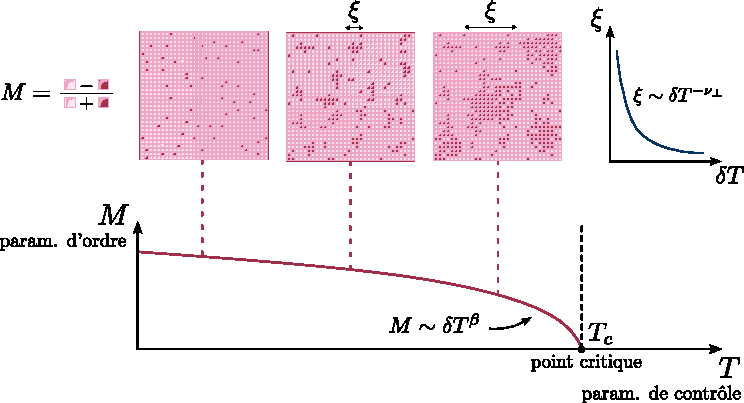
\includegraphics[width=\textwidth]{Chapitre1/Figures/PhenomenesCritiques/PT_conceptCorrLength_fuse.pdf}
	\caption{Illustration de la phénoménologie générale d'une transition de phase via l'exemple de la transition ferromagnétique-paramagnétique.}
	\label{fig:Ising}
\end{figure}

\subparagraph{}Pour conceptualiser le problème, il est d'usage de définir une grandeur, appelée paramètre d'ordre, qui prend des valeurs distinctement différentes dans chacune des phases. La transition se traduit alors par un changement abrupt du paramètre d'ordre autour de la valeur critique du paramètre de contrôle. Dans le cadre de la transition ferromagnétique-paramagnétique, le paramètre d'ordre du système est son aimantation $M$ et le paramètre de contrôle est sa température $T$, dont la valeur critique est la température de Curie $T_c$. Lorsque le matériau est porté à une température $T>T_c$, la phase dominante est la phase paramagnétique, caractérisée par $M=0$, et lorsque celui-ci est refroidi à $T<T_c$ la phase dominante est la phase ferromagnétique, caractérisée par $M\neq 0$ (voir \autoref{fig:Ising}). Le domaine d'étude des phénomènes critiques consiste alors à comprendre l'évolution du système et des quantités le caractérisant près de ce point de transition. Dans la suite de cette sous-section, pour plus de clarté, nous conserverons les notations issues de la transition ferromagnétique-paramagnétique pour développer les concepts associés aux phénomènes critiques.

\subsubsection{Hypothèse de scaling}

\subparagraph{}Afin d'opérer des changements macroscopiques aussi drastiques au cours d'une légère modification du paramètre de contrôle, les entités microscopiques constituant le système doivent coopérer largement proche de la transition. C'est en effet ce que l'on observe : à mesure que l'on s'approche de la transition, la longueur de corrélation $\xi$ associée au système augmente, comme schématisé à la \autoref{fig:Ising}. Au point de transition, aussi appelé point critique, celle-ci diverge.

\subparagraph{}En accord avec ces observations, l'hypothèse de scaling généralisée est une hypothèse fondatrice de l'étude des phénomènes critiques qui permet de comprendre leur phénoménologie \cite{kardar_statistical_2007}. Celle-ci repose sur le fait que, dans le régime critique (i.e. suffisamment proche de la transition), la longueur de corrélation est la seule échelle de longueur pertinente pour décrire le système. En d'autres termes, tous les détails microscopiques du système en-dessous de l'échelle de longueur représentée par $\xi$ sont d'intérêt négligeable. De plus, cette hypothèse suppose que cette longueur de corrélation est une fonction homogène de la distance au point critique :

\begin{equation}
    \xi = \lambda^{\nu_\perp} \tilde{\xi}(\lambda \delta T), \quad \delta T = \frac{T_c-T}{T_c}, \quad \lambda>0.
    \label{eq:homcorr}
\end{equation}

\noindent Le propre d'une fonction homogène étant  que l'\autoref{eq:homcorr} est valide pour tout $\lambda$\footnote{à condition de rester bien sûr dans le domaine critique.}, en prenant $\lambda = 1/\delta T$ nous obtenons :

\begin{equation}
    \xi = \delta T^{-\nu_\perp}\tilde{\xi}(1).
\end{equation}

\noindent Cela retranscrit alors bien le fait que la longueur de corrélation diverge algébriquement avec la distance au point critique.

\begin{figure}[h]
	\centering
	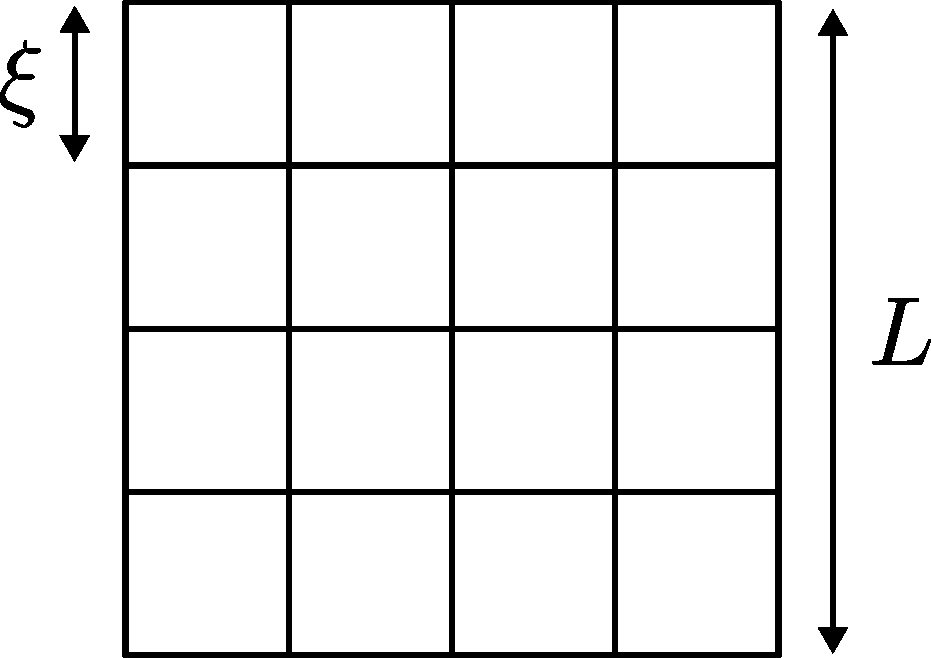
\includegraphics[width=0.3\textwidth]{Chapitre1/Figures/PhenomenesCritiques/decoupageXI.pdf}
	\caption{Découpage schématique d'un système de dimension $L^D$ en une collection de sous-systèmes de dimension $\xi^D$.}
	\label{fig:DecoupageXi}
\end{figure}

\subparagraph{}Cette hypothèse implique un résultat important. Considérons un système de taille $L^D$ que l'on subdivise en un ensemble de sous-compartiments de dimension $\xi^D$, comme représenté à la \autoref{fig:DecoupageXi}. Par définition de la longueur de corrélation, chacun de ces sous-compartiments peut être considéré comme indépendant. Chacun de ceux-ci, au nombre de $\left(\frac{L}{\xi}\right)^D$ contribue à l'énergie libre $f$ du système par la même quantité. En d'autres termes, la partie singulière (associée à la transition) de $f$ se comporte comme $\xi^{-D}$. C'est donc aussi une fonction homogène :

\begin{equation}
    f = \lambda^{y_f}\tilde{f}(\lambda \delta T), \quad \lambda > 0,
\end{equation}

\noindent et dont l'exposant caractéristique est relié au précédent par la relation $y_f = - \nu_\perp D$, génériquement appelée relation d'échelle. 

\subparagraph{}La force de la théorie d'échelle vient alors du point suivant. Les dérivées ou transformées de Legendre d'une fonction homogène sont elles-mêmes des fonctions homogènes. Par ailleurs, celles de l'énergie libre (ou autre potentiel thermodynamique considéré en fonction du système) correspondent à différentes grandeurs physiques d'intérêt. Cela signifie donc que sous cette hypothèse, dans le régime critique, la plupart des quantités décrivant le système sont des fonctions homogènes dont les exposants associés sont liés par des lois d'échelle. Proche du point critique, les observables telles que $\xi$ évoluent donc sans échelle caractéristique, selon des lois de puissance définissant ce qu'on appelle des exposants critiques. Notamment, via le temps de corrélation $\tau$ et la valeur moyenne du paramètre d'ordre $\langle M \rangle$, nous définissons, en plus de $\nu_\perp$, les exposants critiques $\beta$ et $\nu_\parallel$ selon :

\begin{equation}
\begin{aligned}
	\langle M \rangle = \lambda^{-\beta} \tilde{M}(\lambda \delta T) &\Rightarrow \langle M \rangle  \sim \delta T^{\beta},\\
	\tau = \lambda^{\nu_\parallel} \tilde{\tau}(\lambda \delta T) &\Rightarrow \tau \sim \delta T^{-\nu_\parallel}.
\end{aligned}
\end{equation}

\subparagraph{}L'hypothèse de scaling ainsi que les relations d'échelle qui en découlent ont été testées expérimentalement de manière exhaustive, plaçant alors la théorie d'échelle comme le pilier de l'étude des phénomènes critiques \cite{lubeck_universal_2004}.

\subsubsection{Universalité}

\label{sec:univcritique}

\paragraph{Principe}

\subparagraph{}Un aspect essentiel de ce cadre d'étude est de considérer que les détails microscopiques des systèmes situés à des échelles inférieures à $\xi$ ne sont pas pertinents pour en décrire la physique. Dans le régime critique où la longueur de corrélation diverge, ceci motive le fait que le comportement d'une transition peut être déterminé simplement par des considérations globales : c'est le principe d'universalité. L'étude des transitions de phase à l'équilibre a renforcé ce principe d'universalité en montrant que des transitions de nature physique complètement différente partageaient le même comportement critique. Il a alors été possible d'élaborer une catégorisation des phénomènes critiques, les regroupant en classes d'universalité définies uniquement par deux aspects simples (lorsqu'on se limite aux interactions à courte portée) : la dimension de l'espace et les symétries du paramètre d'ordre \cite{kardar_statistical_2007}. Par exemple, la transition ferromagnétique-paramagnétique des matériaux avec un seul axe privilégié d'aimantation appartient à la classe d'universalité d'Ising au même titre que la transition liquide-gaz ou celle de démixtion des liquides binaires \cite{lubeck_universal_2004}. En pratique, cette catégorisation passe par la mesure des exposants critiques, dont chaque ensemble caractérise une unique classe d'universalité.

\paragraph{Théorie continue}

\subparagraph{}Le fait qu'un comportement critique dépende uniquement de critères très généraux motive l'étude de ces phénomènes via des modélisations continues simples sous-forme d'équations de champ.  Par exemple, celle associée à la classe d'Ising est la suivante :

\begin{equation}
	\partial_t \phi (\mathbf{r}, t) = -r\phi (\mathbf{r}, t) + u \phi^3(\mathbf{r}, t) + \kappa\nabla^2 \phi (\mathbf{r}, t) + \sigma\eta(\mathbf{r}, t),
\end{equation}

\noindent avec $\eta$ représentant les fluctuations via un bruit gaussien défini selon :

\begin{equation}
\langle \eta(\mathbf{r}, t) \rangle = 0, \quad \langle \eta(\mathbf{r}, t) \eta(\mathbf{r}^\prime, t^\prime)\rangle = \delta(\mathbf{r}-\mathbf{r}^\prime)\delta(t-t^\prime),
\label{eq:phi4}
\end{equation}

\noindent $\phi$ représentant une version gros grains locale du paramètre d'ordre et $r$ la distance au point critique. Cette théorie continue est connue sous le nom de théorie $\phi^4$ \cite{kardar_statistical_2007}.

\subparagraph{}Dans la limite où les fluctuations de la dynamique sont négligeables, la criticalité décrite par cette équation peut être appréhendée dans son approximation de champ moyen :

\begin{equation}
	\partial_t \phi = -r\phi + u\phi^3 \xrightarrow[r>0]{t\rightarrow \infty} \phi = \left( \frac{r}{u} \right)^\frac{1}{2},
\end{equation}

\noindent menant donc à $\beta^\text{CM} = \frac{1}{2}$. Cependant cette approximation n'est valable que dans certains cas.

\subparagraph{}Dans l'idée que les détails microscopiques ne sont pas pertinents dans le régime critique, nous pouvons redimensionner les distances dans cette équation selon $\mathbf{r}\rightarrow b\mathbf{r}$ avec $b>1$. Sous cette transformation, d'après la théorie d'échelle, les différentes quantités de l'équation sont transformées selon :

\begin{equation}
	\mathbf{r}\rightarrow b\mathbf{r}, \quad t \rightarrow b^{\nu_\parallel/\nu_\perp}t, \quad \phi \rightarrow b^{-\beta/\nu_\perp}\phi,
\end{equation}

\noindent si bien que ce redimensionnement revient à obtenir une équation équivalente à l'\autoref{eq:phi4} avec un redimensionnement des constantes selon :

\begin{equation}
	r \rightarrow b^{\nu_\parallel/\nu_\perp} r, \quad u \rightarrow b^{\nu_\parallel/\nu_\perp - 2\beta/\nu_\perp} u, \quad \kappa \rightarrow b^{\nu_\parallel/\nu_\perp-2}\kappa, \quad \sigma \rightarrow b^{\nu_\parallel/2\nu_\perp+\beta/\nu_\perp - D/2}\sigma.
\end{equation}

\noindent \`A grande échelle ($b\rightarrow\infty$), les fluctuations sont donc négligeables seulement pour $D > (2\beta+\nu_\parallel)/\nu_\perp$. Par ailleurs, dans ce cas champ moyen, l'invariance d'échelle du système au point critique ($r=0$) impose la valeur des exposants $\nu_\parallel^\text{CM} = 1$ et $\nu_\perp^\text{CM} = \frac{1}{2}$. Ce raisonnement définit donc une dimension critique supérieure du système $D_c = 4$ au-delà de laquelle la criticalité décrite par l'équation \autoref{eq:phi4} est triviale\footnote{Nous réutiliserons ce raisonnement générique pour caractériser les propriétés champ moyen d'autres théories dans la suite de cette thèse.}. 

\subparagraph{}En-dessous de cette dimension critique supérieure ($D<D_c$), on ne peut plus négliger les fluctuations dans le système : c'est là que toute la complexité des comportements critiques entre en jeu. Pour étudier le comportement de la théorie de champ à grande échelle dans ce cas, des outils théoriques ont été mis en place. Ceux-ci font intervenir le formalisme associé au groupe de renormalisation. Grâce à ces techniques, il est possible de prédire, au moins perturbativement, les valeurs des exposants critiques associés à une théorie de champ à basse dimension, et donc prédire la criticalité de toute une catégorie de systèmes.

\subparagraph{}En conclusion, les phénomènes critiques à l'équilibre sont caractérisés par des évolutions algébriques des quantités physiques. Ces évolutions sont décrites par différents exposants critiques, reliés par des relations d'échelle. Différentes transitions de phase peuvent être regroupées en une classe d'universalité, décrite par un ensemble de valeurs des exposants critiques. Pour étudier l'universalité de ces classes, il est d'usage de faire appel aux théories de champ continues associées, dont la résolution fait intervenir des outils complexes en-dessous de la dimension critique supérieure.

\subsection{Transitions de phase absorbantes}

\subparagraph{}Après avoir rappelé les bases de la théorie des phénomènes critiques à l'équilibre, nous proposons dans cette sous-section de décrire la phénoménologie propre aux transitions de phase absorbantes. Ces phénomènes hors d'équilibre concernent plus spécifiquement notre étude puisque nous verrons que les transitions de réversibilité et d'écoulement en sont des représentantes. Pour ce faire, nous en proposerons une définition, que nous compléterons ensuite par quelques exemples. Puis, nous présenterons les exposants critiques pertinents pour caractériser ces transitions et la classe d'universalité principale associée.

\subsubsection{Définition}

\subparagraph{}Les transitions de phase absorbantes prennent place dans des systèmes présentant des états absorbants. Ceux-ci correspondent à des états accessibles à la dynamique du système mais dans lesquels celle-ci se retrouve piégée à jamais \cite{lubeck_universal_2004}. Dans une telle transition, le paramètre de contrôle que l'on notera d'abord génériquement $p$ permet de séparer une phase active d'une phase absorbante par sa valeur critique $p_c$. Dans la phase active $p>p_c$, la dynamique du système à temps long est caractérisée par une valeur moyenne positive du paramètre d'ordre $A$, appelé génériquement activité. Dans la phase absorbante $p<p_c$, le système tombe dans un état absorbant au bout d'un temps fini, caractérisé par une activité nulle $A=0$. 

\subparagraph{}La notion d'activité dans ce cadre ne tisse pas de liens avec celle de l'activité dans le contexte de la matière active. Dans une transition de phase absorbante, l'activité correspond plutôt à un état des agents microscopiques qui peut prendre différentes formes selon les systèmes spécifiques considérés.

\subsubsection{Exemples}

\subparagraph{}Sous le point de vue adéquat, de nombreux systèmes peuvent être compris comme des transitions de phase absorbantes. Un exemple incontournable à l'aune de notre époque est celui des épidémies, dans lequel un agent pathogène (virus, bactérie, ...) se propage au sein d'une population \cite{hinrichsen_non_equilibrium_2000, dickman_nonequilibrium_2002, lubeck_universal_2004}. Au premier ordre, on peut modéliser ce système comme à la \autoref{fig:KirbyetArbres}. La population peut alors contenir deux types d'individus : des individus malades, susceptibles de transmettre la maladie à un taux $\lambda$ et de s'en rétablir à un taux $\gamma$, et des individus sains, susceptibles d'être infectés. En fonction de la transmissibilité du virus $\lambda$ et de la capacité de guérison de la population $\gamma$, le système peut connaître deux sorts à temps long : pour $\lambda/\gamma$ suffisamment grand, l'épidémie persistera à temps long alors que pour $\lambda/\gamma$ suffisamment petit, tous les individus finiront par devenir sains. Un tel état est alors un état absorbant puisque dès lors que l'agent pathogène n'a plus de vecteur, il ne peut plus se propager. Dans ce système, on retrouve donc une transition de phase absorbante de paramètre de contrôle $p = \lambda/\gamma$ et dont l'activité correspond à la proportion de personnes infectées dans la population.

\subparagraph{}Un autre exemple pouvant présenter une dynamique tout à fait similaire est celui des feux de forêt \cite{albano_spreading_1995} (voir \autoref{fig:KirbyetArbres}). De la même manière, nous pouvons modéliser ce système au premier ordre par une population d'arbres existant sous deux états possibles : des arbres en feu susceptibles de provoquer l'embrasement d'autres à un taux $\lambda$ et de s'éteindre à un taux $\gamma$, et des arbres sains, seulement susceptibles de prendre feu. Ici encore, selon la valeur du paramètre $p = \lambda/\gamma$, l'état du système à temps long peut prendre deux formes : incendié pour $p>p_c$ et éteint pour $p<p_c$. La forêt sans aucun arbre en feu correspond alors à un état absorbant du système, puisqu'une fois dans cet état, le feu ne peut plus se propager. Dans ce système l'activité correspond à la proportion d'arbres en feu dans la forêt.

\begin{figure}[h]
	\centering
	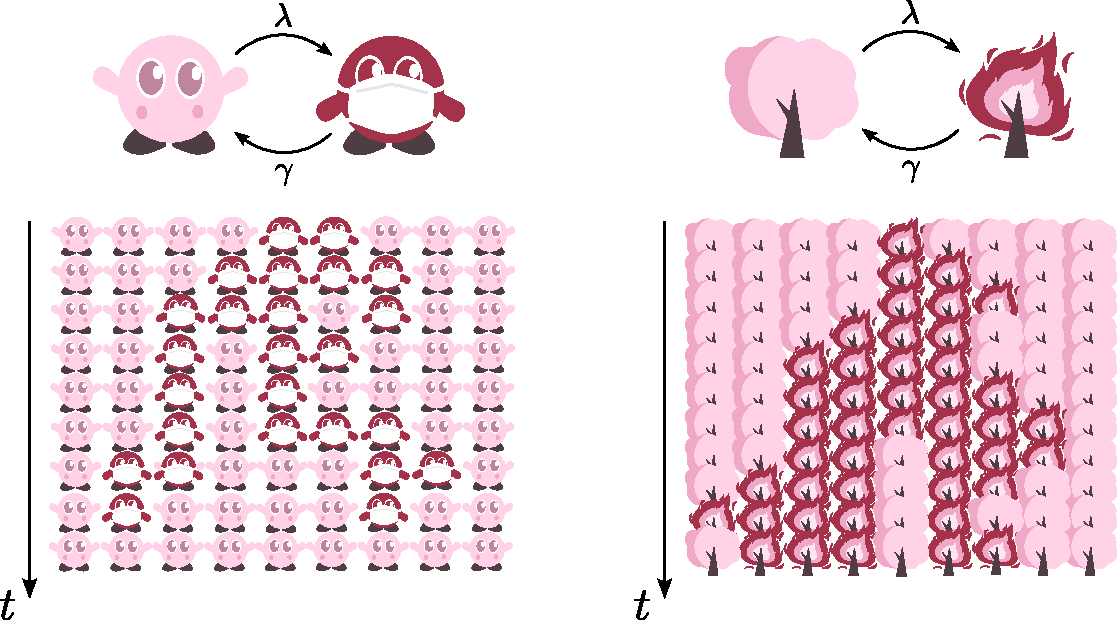
\includegraphics[width=\textwidth]{Chapitre1/Figures/TphiAbs/Kirbies.pdf}
	\caption{Exemples de phénomènes présentant des transitions de phase absorbantes : la propagation des épidémies et les feux de forêts.}
	\label{fig:KirbyetArbres}
\end{figure}

\subparagraph{}De manière générale, de nombreux systèmes peuvent être compris comme des transitions de phase absorbantes s'ils sont observés sous le bon angle. Comme le montrent les exemples précédents, les ingrédients principaux nécessaires à cette dynamique sont une activité microscopique susceptible de se propager comme de s'atténuer et l'existence d'un état bloqué de la dynamique globale.

\subsubsection{Exposants critiques}

\label{sec:tphiexp}

\subparagraph{}Les transitions de phase absorbantes sont des phénomènes hautement hors d'équilibre puisque la présence d'états absorbants implique, par définition, la violation du principe de bilan détaillé. Toutefois, il se trouve que la phénoménologie observée de ces transitions présente de nombreuses similarités avec celle de leurs homologues d'équilibre. Notamment, nous y retrouvons la notion d'homogénéité, d'exposants critiques et d'universalité. Concernant les exposants critiques associés aux transitions de phase absorbantes, ceux-ci peuvent être catégorisés en deux types : ceux reliés à l'état stationnaire de l'activité dans le système, que l'on appellera statiques, et ceux reliés à l'état transitoire ou à des corrélations à deux ou plusieurs temps dans l'état stationnaire, que l'on appellera dynamiques.

\begin{figure}[h]
	\centering
	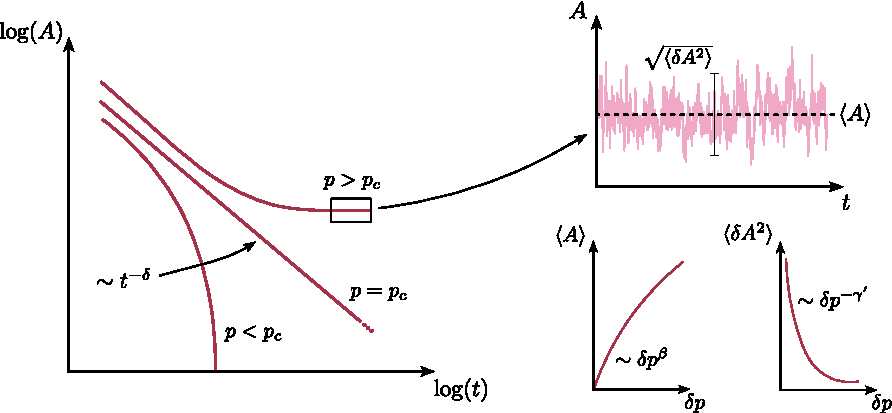
\includegraphics[width=\textwidth]{Chapitre1/Figures/TphiAbs/expabs.pdf}
	\caption{Phénoménologie et définition des différents exposants critiques pertinents dans le cadre des transitions de phase absorbantes.}
	\label{fig:expabs}
\end{figure}

\subparagraph{}Du côté des exposants statiques, nous retrouvons naturellement l'exposant $\beta$ reliant la valeur moyenne de l'activité dans l'état stationnaire à la distance au point critique, et l'exposant $\nu_\perp$ caractérisant la divergence de la longueur de corrélation $\xi$ :

\begin{equation}
	\langle A \rangle \sim \delta p^\beta, \quad \xi \sim \delta p^{-\nu_\perp}, \quad \delta p =  \frac{p-p_c}{p_c}.
\end{equation}

\noindent De plus, nous nous intéresserons aussi dans ce travail à l'évolution des fluctuations du paramètre d'ordre dans l'état stationnaire. Pour un système de taille $L^D$, avec $D$ la dimension du système, nous les caractérisons via la variance $\langle \delta A^2\rangle  = L^D\times(\langle A ^2 \rangle - \langle A \rangle^2)$ dont l'évolution est alors dictée par l'exposant $\gamma^\prime$ :

\begin{equation}
	\langle \delta A^2\rangle \sim \delta p^{-\gamma^\prime}.
\end{equation}

\noindent Le signe apposé à la définition de cet exposant vient du fait qu'en général les fluctuations du paramètre d'ordre divergent à l'approche du point critique, signe d'une dynamique de plus en plus corrélée. En-dessous de la dimension critique $D_c$, les exposants $\beta$, $\gamma^\prime$ et $\nu_\perp$ sont liés par une relation d'échelle :

\begin{equation}
	2\beta + \gamma^\prime = \nu_\perp D,
\end{equation}

\noindent appelée relation d'hyperscaling \cite{lubeck_universal_2004}. Nous ferons appel à cette relation d'échelle à plusieurs reprises dans les différents chapitres de ce manuscrit.

\subparagraph{}Du point de vue dynamique, il existe deux façons principales de caractériser une transition de phase absorbante \cite{lubeck_universal_2004}. La première est de partir d'un état initial avec une zone localisée d'activité, comme c'est le cas sur la \autoref{fig:KirbyetArbres}, et d'étudier la propagation de l'activité dans le système. Une autre possibilité, que nous favoriserons par la suite, est de caractériser la relaxation du système à partir d'un état aléatoire. Dans ce cas, au point critique, la valeur instantanée de l'activité dans le système décroît à temps long de manière algébrique, définissant l'exposant dynamique $\delta$ :

\begin{equation}
	A(t) \sim t^{-\delta}.
\end{equation}

\subparagraph{}Les exposants $\beta$, $\gamma^\prime$ et $\delta$ ainsi définis et illustrés sur la \autoref{fig:expabs} permettent de caractériser une transition de phase absorbante sous différents aspects et de manière unique. 

\subsubsection{Classes d'universalité}

\subparagraph{}Comme à l'équilibre, un grand nombre de transitions de phase absorbantes se regroupent sous forme de classes d'universalité représentées par des valeurs communes des exposants critiques. Dans ce cas hors d'équilibre, la classe d'universalité la plus importante, de manière analogue à la classe d'Ising, est celle de la percolation dirigée (DP) \cite{hinrichsen_non_equilibrium_2000,lubeck_universal_2004}. 

\subparagraph{}Sa dénomination vient de la transition géométrique bien connue qui la représente. Dans le cas de la transition de percolation isotrope, rappelée à la \autoref{fig:percol}-(a), deux sites voisins d'un réseau de $D$ dimensions sont reliés avec une probabilité $p$. Une valeur critique $p_c$ de cette probabilité sépare alors statistiquement deux états du système : pour $p<p_c$ les clusters formés par les liens sont de taille finie tandis que pour $p>p_c$ ceux-ci s'étendent dans tout le système : on dit qu'ils percolent. La percolation dirigée est représentée par le même phénomène, simplement dans ce cas les liaisons entre sites ne peuvent se faire que dans une direction privilégiée (voir \autoref{fig:percol}-(a)). Dans ce cas, les issues possibles en fonction de la valeur du paramètre $p$ sont représentées graphiquement en 2D sur la \autoref{fig:percol}-(b). Nous pouvons alors remarquer de fortes similarités entre la \autoref{fig:percol}-(b) et la \autoref{fig:KirbyetArbres}. En fait, comme lae lecteurice l'aura sûrement déjà compris, les processus absorbants simples présentés précédemment sont équivalents à un phénomène de percolation dirigée, mais dont le temps équivaut à une dimension, soit en $D+1$ dimensions. Une valeur finie de l'activité à temps long dans ces processus correspond alors à la percolation du système tandis que la tombée dans un état absorbant représente la phase non-percolante. Cette équivalence fait que tous ces systèmes sont caractérisés par le même comportement critique : celui de la classe DP.

\begin{figure}[h]
	\centering
	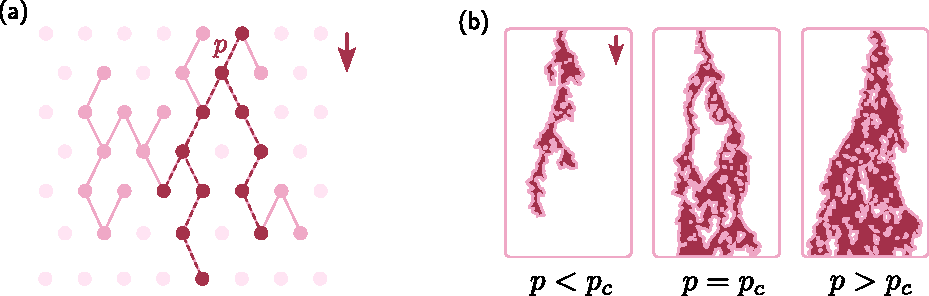
\includegraphics[width=\textwidth]{Chapitre1/Figures/CDP/Percol.pdf}
	\caption{Transition de percolation et de percolation dirigée en 2D. (a) Règles associées à la percolation isotrope (lien roses) et à la percolation dirigée (liens rouges) dont la direction privilégiées est donnée par la flèche. (b) États du système en fonction de la valeur du paramètre de liaison $p$. Pour $p\geq p_c$ le système percole.}
	\label{fig:percol}
\end{figure}

\subparagraph{}Beaucoup d'autres systèmes avec des dynamiques plus complexes ont été caractérisés comme appartenant à la classe DP. Cette ubiquité a motivé une conjecture simple d'appartenance formulée par Janssen et Grassberger \cite{janssen_nonequilibrium_1981, grassberger_phase_1982} : les systèmes présentant une transition de phase absorbante continue vers un unique état absorbant, faisant intervenir des interactions à courte portée et aucune symétrie particulière, appartiennent à la classe DP.

\subparagraph{}D'un point de vue des processus plus abstraits de réaction-diffusion \cite{tauber_applications_2005}, les modèles sur réseaux appartenant à la classe DP peuvent être modélisés par deux processus, un de création et un d’annihilation :

\begin{equation}
A \xrightarrow[]{\lambda} 2A, \quad A \xrightarrow[]{\gamma} \o,
\label{eq:ReacDiffDP}
\end{equation}

\noindent avec $A$ une espèce représentant les agents actifs. Via cette approche il est possible d'associer, comme pour la classe d'Ising, une théorie de champ à la classe DP\footnote{Il est aussi possible de définir un tel processus dans l'espace continu, simplement dans ce cas l'espèce $A$ diffuse avec un coefficient de diffusion $D_A$, et une réaction d'annihilation du type $2A \xrightarrow[]{\gamma^\prime} \o$ est nécessaire pour obtenir un terme de saturation dans l'\autoref{eq:eqDP} (émergeant du principe d'exclusion associé au réseau sinon).} :

\begin{equation}
	\partial_t A(\mathbf{r}, t) = rA(\mathbf{r}, t) - uA^2(\mathbf{r}, t) + \kappa\nabla^2 A (\mathbf{r}, t) + \sigma \sqrt{A(\mathbf{r}, t)} \eta(\mathbf{r}, t),
	\label{eq:eqDP}
\end{equation}

\noindent avec la particularité de faire intervenir un bruit multiplicatif (i.e. dépendant de $A$) qui permet de préserver l'existence d'un état absorbant (pour $A=0$, il n'y a plus de fluctuations). Sa forme en $\sim \sqrt{A}$ vient de la stochasticité des réactions, dont la variance est proportionnelle au nombre d'agents microscopiques.  Par une approche d'échelle identique à celle présentée dans le cadre de la théorie de champ de la classe d'Ising, il est possible de déterminer la valeur champ moyen des exposants critiques en-dessous de la dimension critique supérieure $D_c = 4$. Celles-ci sont reportées dans le \autoref{tab:expocrit_DPCDP}. Via des mesures numériques sur des modèles, ou des approches analytiques sur la théorie de champ, la classe DP a aussi été caractérisée précisément en dimension finie. Notamment, nous reportons la valeur des exposants critiques associés en 2D dans le \autoref{tab:expocrit_DPCDP}.

\begin{table}[h]
\centering
\begin{tabular}{ccccc}
\hline \hline Classe & $\beta$ & $\gamma^\prime$ & $\delta$ & $\nu_\perp$ \\
\hline 
\text{DP (en 2D)} & 0.58 & 0.30 & 0.45 & 0.73 \\
\text{CDP (en 2D)} & 0.64 & 0.37 & 0.42 & 0.80 \\
\text{DP/CDP champ moyen} & 1 & 0 & 1 & 0.5 \\
\hline \hline
\end{tabular}
\caption{Valeurs des exposants critiques associés aux classes d'universalité DP et CDP, en 2D et en champ moyen \cite{lubeck_universal_2004}.}
\label{tab:expocrit_DPCDP}
\end{table}

\subparagraph{}Si DP est la classe la plus répandue et la plus caractérisée aussi bien numériquement qu'analytiquement, il existe d'autres classes, cousines de cette première, correspondant à l'ajout d'ingrédients supplémentaires dans les modèles associés. Notamment, celle d'intérêt pour ce travail est celle de la percolation dirigée conservée (CDP), puisqu'elle représente une dynamique très proche de celles mises en place dans la transition de réversibilité et dans la transition vers l'écoulement.

\section{Percolation dirigée conservée}

\subparagraph{}Dans cette section, nous présentons la classe d'universalité CDP de manière exhaustive puisque, comme nous le verrons, elle représente un premier cadre de compréhension des transitions de réversibilité et d'écoulement. De ce fait, cette partie nous permet d'introduire différent concepts comme les dynamiques d'avalanche ou la notion d'hyperuniformité qui nous seront utiles pour caractériser ces transitions d'intérêt. Pour ce faire, nous commencerons tout d'abord par donner les conditions d'appartenance à la classe CDP et les modèles minimaux qu'elle représente. Ensuite, nous introduirons la transition de dépiégeage comme représentante incontournable de cette classe en présentant la riche phénoménologie qui lui est associée. Par correspondance, nous montrerons alors comment la physique de la transition de dépiégeage se retrouve dans les autres modèles théoriques de type CDP. Cela nous permettra de montrer toute la complexité présente dans cette classe d'universalité que l'on retrouvera en partie lors de l'étude des transitions de réversibilité et d'écoulement.

\subsection{Conditions d'appartenance}

\subparagraph{}La classe CDP se démarque de la classe DP par la présence d'un couplage de la dynamique de l'activité à une quantité conservée et d'un nombre infini d'états absorbants. \`A la façon de la conjecture proposée dans le cas de la classe DP, Rossi et al. \cite{rossi_universality_2000} en ont définie une dans le cadre de la classe CDP : tout système stochastique présentant un nombre infini d'états absorbants dans lequel l'activité est couplée à un champ conservé non-diffusif appartient à la classe CDP. \`A cette conjecture s'ajoute implicitement la condition d'interactions uniquement locales, comme formulé dans la conjecture de Grassberger pour la classe DP \cite{grassberger_phase_1982}.

\subparagraph{}Pour comprendre les éléments de cette distinction, il est plus simple de passer directement par la présentation de modèles appartenant à cette classe d'universalité.

\subsection{Modèles représentatifs}

\label{sec:modelesCDP}

\subsubsection{Modèle Manna}

\subparagraph{}Le modèle Manna \cite{manna_two_state_1991} est un modèle emblématique de la classe CDP, si bien qu'il lui en donne parfois le nom (classe d'universalité Manna) \cite{lubeck_universal_2004}. Dans ce modèle, $N$ particules sont disposées sur $L^D$ sites d'un réseau $D$-dimensionnel, chacun de ces sites pouvant accueillir un nombre arbitraire $n$ de particules. De manière générale, ces particules peuvent aussi bien représenter des grains de sable que des paquets d'énergie. La règle dynamique d'un pas de temps à l'autre de l'évolution est alors la suivante : chaque site du réseau accueillant plus de $m$ particules les redistribue aléatoirement aux sites voisins (voir \autoref{fig:Manna}). Ces sites redistribuant la masse qu'ils supportent sont considérés comme actifs.

\begin{figure}[h]
\centering
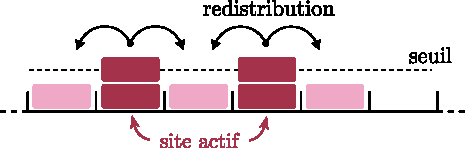
\includegraphics[width=0.6\textwidth]{Chapitre1/Figures/CDP/Manna.pdf}
\caption{Représentation schématique de la dynamique du modèle Manna en 1D. Ici le seuil est fixé à $m=2$.}
\label{fig:Manna}
\end{figure}

\subparagraph{}Sous cette action, les sites sur lesquels a été redistribuée la masse sont susceptibles de dépasser le seuil local $m$ et de devenir actifs à leur tour, menant à une propagation de l'activité dans le système. Ce système présente alors une transition de phase absorbante bien étudiée, dont la densité d'agents $\phi = N/L^D$ est le paramètre de contrôle et dont l'activité $A$ correspond à la proportion de sites actifs du réseau. Pour $\phi > \phi_c$, le système évolue d'un pas de temps à l'autre à travers des configurations avec toujours un excès de particules sur certains sites et donc des redistributions de masse ($A>0$). Cependant, pour $\phi < \phi_c$, le système finit par tomber à temps long dans un état où tous les sites sont inactifs et donc d'activité nulle $A=0$. Un tel état est un état absorbant puisque dès lors qu'aucune redistribution n'a lieu, aucun site ne peut devenir actif. 

\subparagraph{}Dans les modèles épidémiques et de feux de forêts présentés précédemment, il existe un unique état absorbant (toute la population est guérie ou toute la forêt est éteinte). Dans le modèle Manna, il en existe plusieurs. En effet, tout état où tous les sites vérifient $n<m$ sont des états absorbants de la dynamique. Dans la limite thermodynamique $L\rightarrow \infty$, il y en a une infinité. Cela remplit donc la première condition de la conjecture de Rossi et al. \cite{rossi_universality_2000}. Par ailleurs, la dynamique d'activité des sites du réseau est couplée à la dynamique des $N$ particules, dont le nombre est conservé à chaque instant. Dans une vision à grande échelle, ces $N$ particules constituent un champ de densité $\rho (\mathbf{r}, t)$ de valeur intégrale constante (donc dit conservé) et évoluant uniquement sous l'action de l'activité (donc dit non-diffusif). Cela remplit donc la seconde condition de la conjecture, faisant du modèle Manna un représentant de la classe CDP. Chronologiquement cependant, c'est en réalité plutôt le modèle Manna qui a permis de définir la classe CDP \cite{lubeck_universal_2004}.

\subsubsection{Random Organization Model}

\subparagraph{}Un second modèle respectant la conjecture de Rossi et al. \cite{rossi_universality_2000} et appartenant à la classe CDP est le Random Organization Model (ROM) \cite{corte_random_2008, tjhung_criticality_2016}. Le ROM est très proche du modèle Manna dans son principe et sa dynamique, à la différence que celle-ci a lieu dans un espace continu.

\begin{figure}[h]
\centering
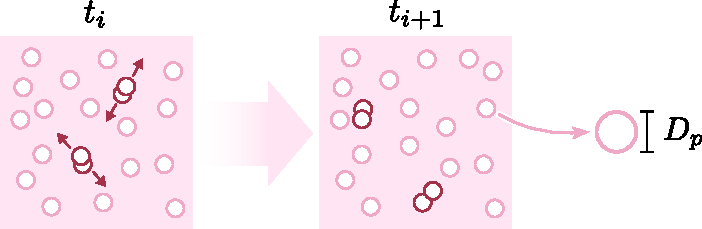
\includegraphics[width=0.85\textwidth]{Chapitre1/Figures/CDP/ROM.pdf}
\caption{Représentation schématique de la dynamique du ROM en 2D.}
\label{fig:ROM}
\end{figure}

\subparagraph{}Dans le cadre de ce modèle, $N$ particules sphériques de diamètre $D_p$ sont positionnées dans un espace de $D$ dimensions et d'extension spatiale $L$. Chacune de ces $N$ particules peut alors prendre deux états à chaque pas de temps : si la particule se recouvre avec une autre particule elle est active, sinon elle est passive. Lorsqu'une particule est active, celle-ci est soumise à un déplacement d'amplitude aléatoire, modifiant sa position dans l'espace continu. Ce déplacement représente alors la possibilité d'un recouvrement avec une nouvelle particule, menant à une potentielle propagation de l'activité dans le système. Cette dynamique présente une transition de phase absorbante dont le paramètre de contrôle est la fraction volumique $\phi$ de particules dans le système et dont l'activité $A$ correspond à la proportion de particules actives. Pour $\phi>\phi_c$, le système traverse des configurations où il existe toujours au moins un recouvrement entre particules ($A>0$). Cependant, pour $\phi<\phi_c$, le système finit par tomber dans une configuration où toutes les particules sont suffisamment éloignées pour qu'aucunes ne se recouvrent ($A=0$). Une telle configuration est un état absorbant puisque sans le déplacement d'une particule active, aucune particule passive ne peut le devenir. 

\subparagraph{}Comme dans le cas du modèle Manna, le ROM possède un nombre infini d'états absorbants. En effet, chaque ensemble de position des particules $\{\mathbf{r}_i\}_{i<N}$ vérifiant $|\mathbf{r}_i-\mathbf{r}_j|<D_p$ pour tout $i\neq j$ est un état absorbant. Les positions étant continues, il y en a une infinité (et pas seulement dans la limite thermodynamique). Le ROM vérifie donc la première condition de la conjecture de Rossi et al. \cite{rossi_universality_2000}. Par ailleurs, de la même manière que dans le modèle Manna, ce modèle fait intervenir la dynamique non-diffusive de $N$ particules dont le nombre est conservé à chaque instant, vérifiant de ce fait la seconde condition de la conjecture. La seule différence ici est que l'activité est aussi représentée par les particules (actives) et non l'espace (comme c'est le cas dans le modèle Manna via la notion de sites actifs). Ce modèle est donc aussi un représentant de la classe CDP.

\subparagraph{}Par définition d'une classe d'universalité le modèle Manna et le ROM sont donc caractérisés par la même théorie sous-jacente, associée à un ensemble cohérent d'exposants critiques.

\subsection{Comportement critique}

\label{sec:CompCDP}

\subparagraph{}Du point de vue des processus de réaction-diffusion, les modèles appartenant à la classe CDP peuvent être ramenés à un processus à deux espèces \cite{van_wijland_wilson_1998, pastor_satorras_reaction_diffusion_2001, pastor_satorras_field_2000} (contrairement à la classe DP qui n'en fait intervenir qu'une) :

\begin{equation}
	A +B \xrightarrow[]{\lambda} 2A, \quad A \xrightarrow[]{\gamma} B,
\end{equation}

\noindent avec l'espèce $A$ diffusant avec un coefficient de diffusion $D_A$ dans le cas continu. Ces deux processus conservent alors le nombre total $N=N_A+N_B$ de particules, comme c'est le cas dans le modèle Manna et le ROM. Via ce formalisme, il est possible de définir une théorie de champ décrivant cette dynamique proche de celle de DP \cite{van_wijland_universality_2002, le_doussal_exact_2015} :

\begin{equation}
\begin{aligned}
	&\partial_t A(\mathbf{r}, t) = (\omega\rho (\mathbf{r}, t) - r)A(\mathbf{r}, t) - uA^2(\mathbf{r}, t) + \kappa\nabla^2 A (\mathbf{r}, t) + \sigma \sqrt{A(\mathbf{r}, t)} \eta(\mathbf{r}, t),\\
	&\partial_t \rho (\mathbf{r}, t) = \kappa\nabla^2 A (\mathbf{r}, t),
\end{aligned}
\label{eq:CDP}
\end{equation}

\noindent avec $\rho(\mathbf{r}, t)$ le champ conservé.

\subparagraph{}Via une analyse d'échelle similaire au cas DP, il est possible de montrer que la classe CDP admet des exposants de champ moyen identiques en-dessous de la même dimension critique supérieure $D_c = 4$ \cite{le_doussal_exact_2015, lubeck_universal_2004}. Ainsi, en champ moyen, les classes DP et CDP sont équivalentes. Pour $D<D_c$ cependant, les mesures numériques sur les différents modèles représentant la classe CDP ont permis de la séparer de son homologue DP. En 2D, les valeurs des exposants déterminés pour cette classe sont reportées dans le \autoref{tab:expocrit_DPCDP}.

\subparagraph{}Comme on peut le remarquer, les exposants critiques caractérisant les deux transitions sont en fait très similaires, avec un écart relatif de seulement quelques pourcents. Cette grande proximité a rendu compliquée la séparation de ces deux classes, qui a alors été un sujet de débats. Toutefois, les techniques numériques actuelles et des arguments analytiques basés sur les techniques du groupe de renormalisation permettent aujourd'hui d'affirmer que ces deux criticalités sont bien distinctes.

\subsection{Classe CDP et transition de dépiégeage}

\subparagraph{}En dehors des modèles de particules comme le modèle Manna ou le ROM, la classe CDP possède une forte représentation, notamment en matière molle, via la transition de dépiégeage. Dans cette sous-section, nous proposons de présenter succinctement la transition de dépiégeage. Pour ce faire, nous en donnerons d'abord une image générale dans le cadre théorique des variétés élastiques. Cela nous permettra d'en décrire la phénoménologie associée, notamment via la rugosité de l'interface et la dynamique d'avalanche. Nous ferons ensuite le parallèle entre transition de dépiégeage et la classe CDP en expliquant l'équivalence récemment mise en évidence entre ces deux objets.

\subsubsection{Phénoménologie de la transition de dépiégeage}

\paragraph{Une transition de phase absorbante}

\subparagraph{}Dans un cadre général, la transition de dépiégeage concerne le mouvement d'une variété élastique de $D$ dimensions dans un milieu désordonné de $D+n$ dimensions \cite{fisher_collective_1998}. Au cours de celui-ci, deux phénomènes entrent en jeu. D'une part, l'élasticité de la variété tend à rapprocher localement chacun de ses points. D'autre part, le milieu désordonné agit sur chaque point de la variété en le piégeant  localement, plus ou moins fortement. L'exemple le plus parlant est celui-ci d'une ligne élastique ($D=1$) se déplaçant sur une interface rugueuse ($n=1$), comme représenté à la \autoref{fig:depinningbase}-(a).

\begin{figure}[h]
	\centering
	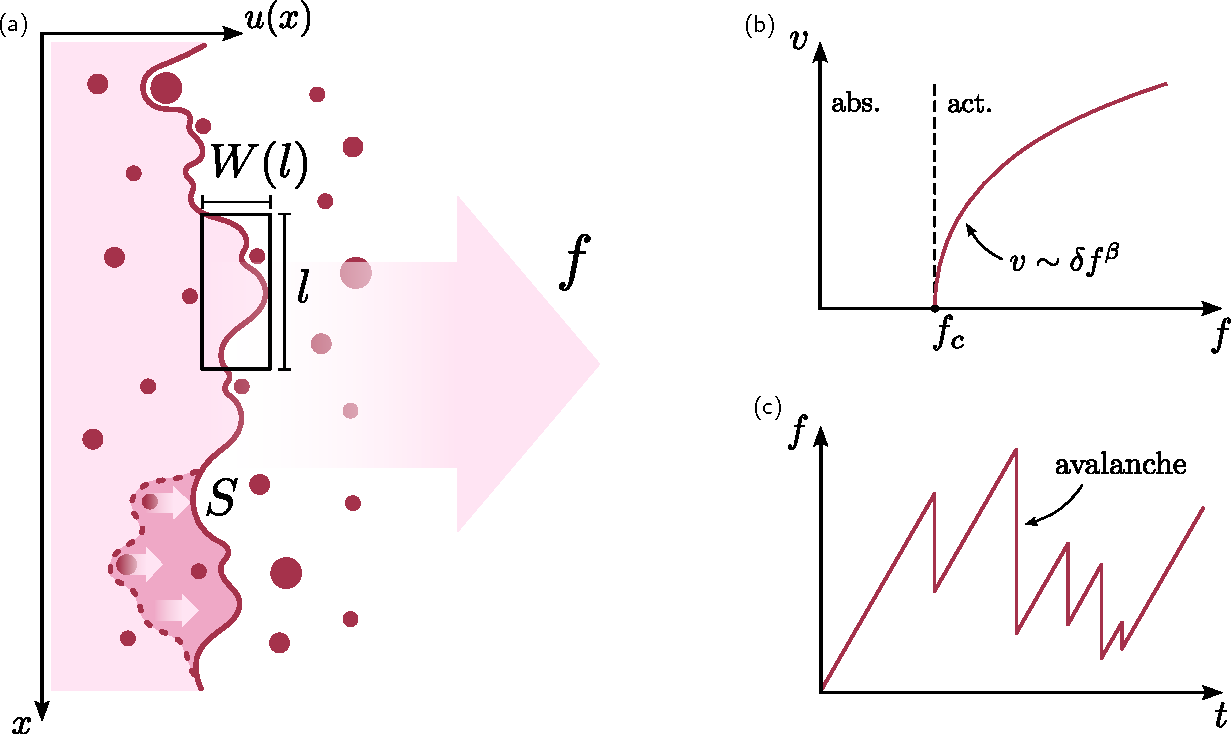
\includegraphics[width=\textwidth]{Chapitre1/Figures/Depinning/depinningbase.pdf}
	\caption{(a) Représentation schématique de la dynamique à l’œuvre dans la transition de dépiégeage en 1D, i.e. dans le cas d'une ligne élastique. Les disques rouges représentent le substrat désordonné. (b) Évolution de la vitesse moyenne de l'interface en fonction de la force appliquée (c) Dynamique d'avalanche dans le cadre d'un processus de forçage-dissipation. Chaque chute de force globale représente une avalanche dans la ligne élastique.}
	\label{fig:depinningbase}
\end{figure} 

\subparagraph{}Sous l'action d'une force extérieure $f$, matérialisée par une densité de force uniforme le long de la ligne,  celle-ci peut se dépiéger localement de l'interaction avec le substrat et se déplacer jusqu'au prochain point de piégeage. Ce déplacement induit une nouvelle configuration de la ligne et modifie alors la force élastique à laquelle sont soumis les autres points. Si l'addition de cette nouvelle force élastique locale et de la force extérieure est suffisamment grande, un autre point de la ligne peut se dépiéger et avancer. Cela constitue un mécanisme de propagation du dépiégeage. Il y a alors deux cas possibles en regard du comportement global de la ligne. Pour une force extérieure suffisamment grande $f>f_c$, le système se dépiège localement en permanence, amenant dans l'état stationnaire à une vitesse moyenne de déplacement de l'interface non-nulle $v>0$. Cependant, pour une force extérieure trop faible $f<f_c$, le système finit par tomber dans un état totalement piégé : localement l'addition de la force extérieure et de la force élastique ne permet pas de contrer la force de piégeage exercée par le substrat. 

\subparagraph{}Cette transition, entre un état mobile et un état piégé, est ce qu'on appelle la transition de dépiégeage. Comme lae lecteurice l'aura sûrement déjà compris, cette transition peut être abordée comme une transition de phase absorbante dont le paramètre de contrôle est la force extérieure $f$ et dont l'activité correspond à la vitesse de l'interface $v$ (localement, un point de l'interface est actif s'il se déplace). 

%L'état piégé correspond effectivement à un état absorbant puisque, en l'absence de fluctuations thermiques que l'on ne considérera pas dans ce travail, il est impossible qu'un point de la ligne se dépiège sans ajout supplémentaire de force.

\subparagraph{}Dans la suite de cette partie, nous présentons deux caractéristiques incontournables de la criticalité associée à la transition de dépiégeage : la rugosité de l'interface et la dynamique d'avalanche.

\paragraph{Rugosité}

\subparagraph{}La compétition complexe entre force de rappel élastique qui tend à aplanir l'interface et force de piégeage qui tend à déformer l'interface rend la structure de cette dernière non-triviale : proche de la transition, elle acquiert une certaine rugosité \cite{fisher_collective_1998, wiese_theory_2022}. La rugosité d'une interface est définie via la largeur $W$ balayée par une portion d'extension $l$ de cette interface (voir \autoref{fig:depinningbase}-(a)). Proche de la transition, $W$ varie algébriquement avec $l$ selon :

\begin{equation}
	W(l) \sim l^\eta,
\end{equation}

\noindent $\eta$ définissant l'exposant de rugosité, un exposant universel au même titre qu'un autre exposant critique. En définissant $u(x)$ la position de l'interface, cette évolution algébrique se retrouve de manière équivalente dans les fluctuations de cette position. En effet, on a directement :

\begin{equation}
	W^2(l) = \overline{\left\langle (u(\mathbf{r}) - \langle u(\mathbf{r}) \rangle)^2\right\rangle} \sim l^{2\eta},
\end{equation}

\noindent où $\langle \cdot \rangle$ désigne la moyenne spatiale sur la portion d'extension $l$ et $\overline{\cdot}$ la moyenne sur les réalisations du désordre. Dans l'espace de Fourier\footnote{Les notations et conventions utilisées dans ce manuscrit pour la transformée de Fourier sont indiquées dans l'\annexeref{sec:conv_fourier}.}, cette propriété se retrouve dans le facteur de structure $S$ : 

\begin{equation}
	S(\mathbf{q}) = \overline{\hat{u}(\mathbf{q})\hat{u}(-\mathbf{q})} \sim q^{-(D+2\eta)}.
\end{equation}

\paragraph{Avalanches}

\subparagraph{}En partant d'une configuration piégée de la ligne élastique et en augmentant lentement la force extérieure $f$ tout en gardant $f<f_c$, la ligne finit par se dépiéger localement, et une portion de celle-ci se déplace avant de se retrouver bloquée à nouveau. Ce saut d'un état absorbant à un autre est ce qu'on appelle une avalanche. Ces objets sont définis par leur taille $S$, correspondant au déplacement moyen de la ligne lors de l'évènement, et leur durée $T$. Proche du point critique $f=f_c$, ces caractéristiques sont distribuées algébriquement selon \cite{narayan_threshold_1993, rosso_avalanche_size_2009, le_doussal_statistics_2009, le_doussal_size_2009, wiese_theory_2022} :

\begin{equation}
P_S(S) \sim S^{-\tau}g_S\left( \frac{S}{S_c} \right), \quad P_T(T) \sim T^{-\tau^\prime}g_T\left( \frac{T}{T_c} \right),
\end{equation}

\noindent avec $g_S(x)$ et $g_T(x)$ constantes pour $x\ll 1$ et à décroissance rapide pour $x>1$, $\tau$ et $\tau^\prime$ définissant des exposants d'avalanche universels. Ces deux quantités peuvent être reliées à l'extension spatiale $l$ de l'avalanche par deux nouveaux exposants critiques :

\begin{equation}
	S \sim l^{d_f}, \quad T \sim l^z,
\end{equation}

\noindent avec $d_f$ la dimension fractale des avalanches et $z$ l'exposant dynamique. Ces deux exposants sont reliés à deux autres exposants présentés précédemment par les relations d'échelle :

\begin{equation}
	d_f = D + \eta, \quad z = \frac{\nu_\parallel}{\nu_\perp}.
\end{equation}

\subparagraph{}Pour $f>f_c$, la dynamique se prolonge indéfiniment et il est donc complexe de séparer les différentes avalanches. Pour analyser les avalanches au-dessus de la force critique il est alors d'usage de procéder d'une manière un peu différente : en plus du mécanisme de forçage, un mécanisme de dissipation est ajouté. Cette fois, en parallèle d'une augmentation constante de $f$, la force extérieure suit une diminution instantanément proportionnelle à l'activité globale dans le système \cite{le_priol_long_range_2020, wiese_theory_2022}. Lorsque l'augmentation de $f$ est suffisamment lente, une séparation d'échelle se crée entre le forçage et la relaxation du système d'un état piégé à un autre. Les évènements de relaxation ainsi désignés sont associés aux avalanches au-dessus du seuil (voir \autoref{fig:depinningbase}-(c)). De la même façon, il est possible d'en caractériser la statistique via la taille et la durée des évènements. Sous ces conditions, le système évolue naturellement vers le point critique $f=f_c$. On parle alors de criticalité auto-organisée (SOC) \cite{bak_self_organized_1988, turcotte_self_organized_1999, lubeck_universal_2004}. Dans ce cadre, les cut-offs des distributions ne dépendent que de l'extension spatiale $L$ du système selon :

\begin{equation}
	S_c \sim L^{d_f}, \quad T_c \sim L^{z}.
\end{equation}

\subsubsection{Mapping avec la classe CDP}

\label{sec:mapping_dep_cdp}

\subparagraph{}L'intérêt de présenter la transition de dépiégeage dans le cadre de notre travail est que toute la richesse de ce phénomène longuement étudié se retrouve dans les modèles appartenant à la classe CDP. En effet, nous présentons dans cette partie les travaux de Le Doussal et Wiese, confirmés par la suite par Janssen et Stenull \cite{janssen_directed_2016}, qui montrent que la transition de dépiégeage peut être directement mise en équivalence avec l'universalité de la percolation dirigée conservée \cite{le_doussal_exact_2015, wiese_hyperuniformity_2024}.

\subparagraph{}La transition de dépiégeage peut être modélisée simplement par une équation du mouvement continue sur la ligne. Dans le cas où l'élasticité de la ligne est à courte portée, celle-ci prend la forme suivante \cite{fisher_collective_1998, wiese_theory_2022} :

\begin{equation}
	\partial_t u (x,t) = (\nabla^2 - m^2)u(x,t) + F(x, u(x,t)) + f(x,t), \quad F(x,u) = - \partial_u V(x,u),
	\label{eq:qEW}
\end{equation}

\noindent avec $u$ la position de l'interface perpendiculairement à l'axe $(Ox)$, $f$ la force extérieure et $F$ la force aléatoire de piégeage, dérivant d'un potentiel désordonné $V$. Dans la limite $m=0$, celle-ci correspond à l'équation de quenched-Edward-Wilkinson \cite{nattermann_dynamics_1992}. Le terme $\nabla^2 u (x,t)$ représente la force élastique de courte portée le long de la ligne. De manière générale, nous pouvons écrire ce terme via la formulation $(\mathcal{G}\ast u) (x,t)$ désignant la convolution du champ de déplacement avec un propagateur de redistribution élastique $\mathcal{G}$. Ceci peut s'avérer utile dans le cas de la généralisation aux interactions à longue portée, discutées dans la suite de cet ouvrage.

\subparagraph{}Par cette formulation, il a été possible de faire une équivalence entre l'\autoref{eq:qEW} et l'\autoref{eq:CDP}, associant alors directement la transition de dépiégeage à la classe d'universalité CDP \cite{le_doussal_exact_2015, wiese_hyperuniformity_2024}. Dans ce cadre, le champ d'activité $A$ correspond naturellement au champ de vitesse de l'interface $\partial_t u$. La correspondance moins évidente que montre cette équivalence est celle entre la densité de particules $\rho(x,t)$ dans la théorie CDP et la force de rappel élastique dans le cadre théorique du dépiégeage :

\begin{equation}
	\rho(x,t) - \rho_0 \sim \nabla^2 u (x,t),
	\label{eq:equivCDPdépiégeage}
\end{equation}

\noindent où $\rho_0$ représente la densité moyenne de particules. Cette correspondance permet de faire un lien entre les deux mécanismes de propagation de l'activité. Dans un modèle de particules comme le modèle Manna, l'activité induit localement une redistribution de la masse (représentée par $\rho(x,t)$), susceptible de générer de l'activité par surcharge de nouveaux sites. De manière équivalente, dans le cas du dépiégeage, l'activité induit localement une redistribution de la force élastique susceptible de générer de l'activité par traction suffisante de nouveaux points de la ligne.

\subparagraph{}L'étude de la transition de dépiégeage via sa théorie continue a été réalisée de manière extensive, numériquement mais aussi analytiquement via la mise en place d'outils du groupe de renormalisation fonctionnel. Cette équivalence permet alors de transposer tous les résultats obtenus à la théorie CDP, comme la valeur des exposants critiques associés. De plus, ce mapping permet de faire le lien entre les différentes propriétés de la transition de dépiégeage et celles des modèles de particules, notamment celles de rugosité et de dynamique d'avalanche. Dans la suite de cette section, nous proposons d'expliciter l'équivalent de ces propriétés dans les modèles de particules puisque ces notions nous seront utiles dans la suite de cette ouvrage.

\subsection{Avalanches}

\label{sec:IntroAvalanches}

\subparagraph{}De la même manière que dans la transition de dépiégeage, il est possible d'observer des avalanches dans les modèles de particules appartenant à la classe CDP \cite{lubeck_moment_2000, dickman_paths_2000}. La façon la plus courante de les étudier est, comme dans le cas du dépiégeage, d'ajouter au modèle une composante de forçage et de dissipation \cite{lubeck_universal_2004}. Prenons l'exemple du modèle Manna. Dans ce cas, le forçage correspond à l'augmentation progressive de la densité de particules, via l'ajout aléatoire à un taux $\kappa$ de particules dans le système. La dissipation correspond, elle, à une disparition des particules sur les sites actifs à un taux $\tau$. Dans la limite $\kappa/\tau \ll 1$, la séparation d'échelle entre le forçage et la dissipation fait place à un phénomène d'avalanche : le système saute d'un état inactif à un autre, via des impulsions d'activité. Via ce processus, le système oscille naturellement autour de sa densité critique $\phi_c$.

\subparagraph{}De la même manière que dans la transition de dépiégeage, ces avalanches peuvent être caractérisées via leur taille et leur durée et les exposants critiques $\tau$, $\tau^\prime$, $d_f$ et $z$ qu'elles définissent. Ces deux transitions étant équivalentes, elles partagent les mêmes valeurs de ces exposants. Dans le cas des modèles de particules, la taille d'une avalanche correspond à la quantité d'activations générées lors de la relaxation $S = \int_0^T \mathrm{d}t~ A(t)$.

\subparagraph{}Dans le cadre de la classe CDP, il est possible de relier les exposants d'avalanches aux exposants critiques dynamiques \cite{munoz_avalanche_1999, lubeck_universal_2004}, reliant sans équivoque la dynamique critique à densité imposée à celle sous le mécanisme de forçage-dissipation. Ainsi, l'étude des avalanches revient à étudier la dynamique de la transition d'un point de vue différent de celui présenté à la \autoref{sec:tphiexp}.

\subsection{Hyperuniformité}

\label{sec:introHU}

\paragraph{Fluctuations de position, fluctuations de densité}

\subparagraph{}La rugosité est une propriété propre aux interfaces. Il n'est donc pas direct de voir comment son aspect critique se transpose aux modèles de particules. En fait, l'équivalence soulignée dans l'\autoref{eq:equivCDPdépiégeage} reliant la densité de particules $\rho$ à la position de l'interface $u$ permet de faire le lien entre fluctuations de position et fluctuations de densité :

\begin{equation}
	\overline{\left\langle (\rho(\mathbf{r}) - \langle \rho(\mathbf{r}) \rangle)^2\right\rangle} \rightarrow \overline{\left\langle (\nabla^2 u(\mathbf{r}) - \langle \nabla^2 u(\mathbf{r}) \rangle)^2\right\rangle} \sim l^{2(\eta-2)},
	\label{eq:MappingHyperuni}
\end{equation}

\noindent avec $l$ l'extension spatiale du domaine considéré pour la mesure des fluctuations. Un exposant de rugosité $\eta$ non-trivial implique donc des fluctuations de densité non-triviales dans les modèles de particules appartenant à la classe CDP. Dans une certaine limite, cette propriété correspond à une hyperuniformité de la répartition de masse dans le système. Pour le comprendre, nous introduisons brièvement ce qu'est l'hyperuniformité dans un cadre général.

\paragraph{Répartition de masse et hyperuniformité}

\subparagraph{}La répartition d'un ensemble de points dans l'espace peut prendre différentes formes, associées à différents types de corrélations. Celle-ci peut aller de la structure cristalline infiniment corrélée au cas aléatoire totalement décorrélé. Une manière de quantifier le degré de corrélation spatiale est d'étudier comment évoluent les fluctuations de densité à différentes échelles du système. 

\subparagraph{}Dans le cas d'une répartition poissonienne totalement décorrélée (voir \autoref{fig:HU}-(b)), la variance $\langle \delta n^2 \rangle$ du nombre $n$ de particules dans un échantillon évolue proportionnellement à son extension spatiale $l^D$. Considérant des répartitions uniformes, on a par ailleurs $\langle n \rangle \sim l^D$. Ainsi dans ce cas décorrélé on a :

\begin{equation}
	\langle \delta n^2 \rangle_l \sim \langle n \rangle_l.
\end{equation} 

\subparagraph{}Dans le cas d'un ordre parfaitement cristallin (voir \autoref{fig:HU}-(a)), la variance $\langle \delta n^2 \rangle$ évolue proportionnellement au périmètre de la zone considérée\footnote{Ceci est valable tant que la forme du domaine n'est pas spécifiquement reliée au motif cristallin.}, lui même évoluant comme $l^{D-1}$. Ainsi, on aura :

\begin{equation}
	\langle \delta n^2 \rangle_l \sim \langle n \rangle_l^{1-1/D}.
\end{equation} 

\subparagraph{}Une évolution non-linéaire de $\langle \delta n^2 \rangle$ avec $\langle n \rangle$ indique la présence de corrélations dans la répartition de la densité dans le système. Si le cas cristallin est le plus extrême, il existe un continuum de répartitions caractérisées par $\langle \delta n^2 \rangle_l \sim \langle n \rangle_l^{\sigma}$, indiquant la présence de corrélations intermédiaires. Dès lors que $\langle \delta n^2 \rangle$ croît moins rapidement que $\langle n \rangle$ avec $l$ (i.e. $\sigma < 1$), on qualifie cette répartition d'hyperuniforme.

\begin{figure}[h]
	\centering
	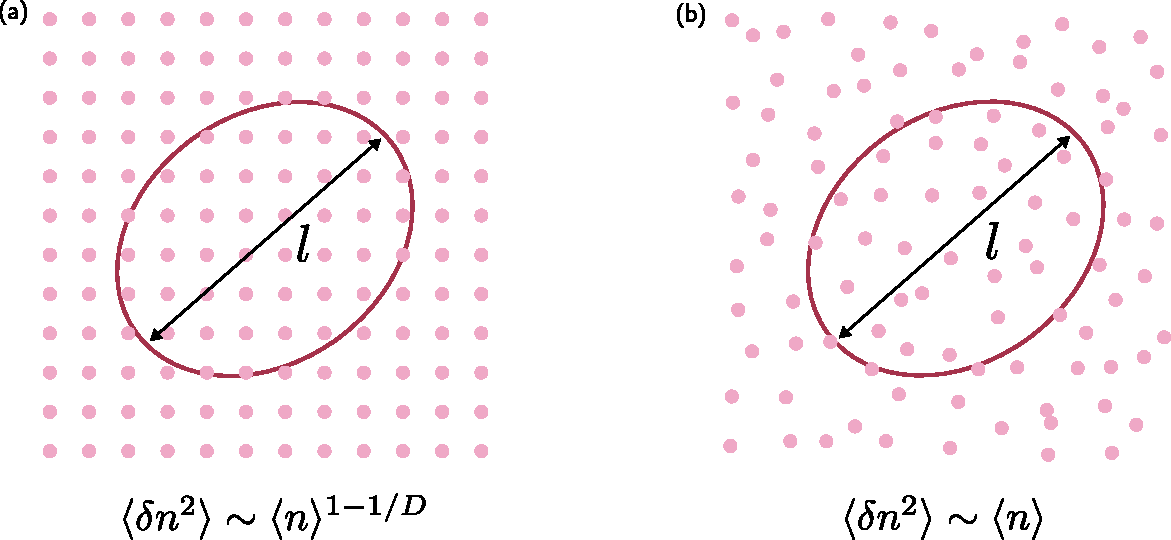
\includegraphics[width=\textwidth]{Chapitre1/Figures/CDP/hyperuniformite.pdf}
	\caption{Répartitions de masse dans le cas cristallin (a) et dans le cas poissonien (b), amenant à des lois d'échelle différentes entre $\langle \delta n^2 \rangle$ et $\langle n \rangle$.}
	\label{fig:HU}
\end{figure}

\paragraph{Hyperuniformité dans les modèles de particules appartenant à la classe CDP}

\subparagraph{}Dans un modèle de particules, il est possible d'associer trivialement les fluctuations de nombre de points/particules aux fluctuations de densité. Ainsi, via l'\autoref{eq:MappingHyperuni}, les exposants $\sigma$ et $\eta$ sont en fait directement liés par la relation d'échelle :

\begin{equation}
	\sigma = 2 + \frac{2\eta - 4}{D}.
	\label{eq:rel_eta_sigma}
\end{equation}

\noindent Un exposant de rugosité $\eta < 1$ dans le modèle de dépiégeage correspond donc de manière équivalente à une répartition hyperuniforme de la masse dans les modèles de particules en 2D. En dimension arbitraire, une évolution hyperuniforme $\sigma < 1$ est associée à un exposant de rugosité $\eta < (4-D)/2$. Cette équivalence est validée par les mesures effectuées sur les modèles numériques. Par exemple, dans le cas du ROM en 2D, il a été mesuré $\sigma \approx 0.775$ \cite{tjhung_hyperuniform_2015, hexner_hyperuniformity_2015, weijs_emergent_2015}.

\subsection{Bilan}

\subparagraph{}En conclusion, la classe d'universalité CDP prétend à représenter tous les modèles présentant une transition de phase absorbante avec une infinité d'états absorbants et impliquant la dynamique d'un champ conservé. Cette classe possède deux représentations principales : les modèles de particules comme le modèle Manna ou le ROM et les modèles de dépiégeage. Les phénomènes apparentés à cette classe présentent une phénoménologie riche, caractérisée par des propriétés hyperuniformes et une dynamique d'avalanche critique. Via l'étude combinée des modèles de particules et de la transition de dépiégeage, le cadre CDP représente un objet d'étude bien balisé, regroupant prédictions théoriques et mesures numériques dans différentes dimensions. L'intérêt d'avoir présenté cette classe exhaustivement est qu'elle correspond en fait à un cadre de description proche des transitions qui motivent ce travail : la transition de réversibilité dans les suspensions cisaillées cycliquement et la transition vers l'écoulement des fluides à seuil. Les aspects spécifiques de la dynamique associée (avalanches, hyperuniformité, ...) se retrouveront donc dans notre étude de ces phénomènes.

\section[Les transitions de réversibilité et d'écoulement comme transitions de phase \\ absorbantes]{Les transitions de réversibilité et d'écoulement comme transitions de phase absorbantes}

\subparagraph{}Dans cette section, nous revenons sur les deux objets d'intérêt de notre travail : la transition de réversibilité dans les suspensions cisaillées cycliquement et la transition vers l'écoulement des fluides à seuil. Pour chacune d'elle, nous explicitons la dynamique sous-jacente à ces transitions et expliquons en quoi celle-ci correspond à celle d'une transition de phase absorbante. Puis, en se basant sur la conjecture de Rossi et al. \cite{rossi_universality_2000}, nous montrons que ces deux systèmes sont proches de ceux représentés par la classe CDP, seulement avec la présence additionnelle d'interactions à longue portée.

\subsection{Transition de réversibilité}

\subparagraph{}Dans la première partie de l'introduction, nous avions présenté la transition de réversibilité dans les suspensions cisaillées cycliquement comme séparant un état réversible, stroboscopiquement arrêté, d'un état irréversible, stroboscopiquement diffusif. Pour comprendre comment ce phénomène peut être appréhendé dans le cadre des transitions de phase absorbantes, il est nécessaire de remarquer comment cette diffusion stroboscopique prend place.

\subsubsection{La diffusion comme une succession d'interactions irréversibles}


\subparagraph{}Dans la limite de bas Reynolds, les équations de Stokes qui gouvernent la dynamique de ce système sont réversibles dans le temps \cite{kimMicrohydrodynamicsPrinciplesSelected1991}. En d'autres termes, si lors de la première moitié d'un cycle une particule n'est déplacée que par les mouvements réversibles du fluide, alors lors de la seconde moitié de ce cycle, elle reviendra à sa position initiale. Toutefois, si au cours de cette première moitié de cycle la particule interagit irréversiblement avec une autre particule à courte portée, cette irréversibilité laissera une trace lors du mouvement retour du fluide. Dans ce cas, la particule ne revient pas à sa position d'origine. Dès lors, une dynamique collective se met en place : une particule qui a changé de position entre le début et la fin d'un cycle va suivre une nouvelle trajectoire, perturbant alors possiblement celle d'une autre particule par une interaction de contact irréversible. De ce fait, cette nouvelle particule change d'orbite et peut perturber l'orbite d'une autre particule à son tour. Ce faisant, ce mécanisme permet une propagation de l'irréversibilité dans le système, d'autant plus efficace que les orbites sont développées et donc l'amplitude de cisaillement globale grande.

\begin{figure}[h]
	\centering
	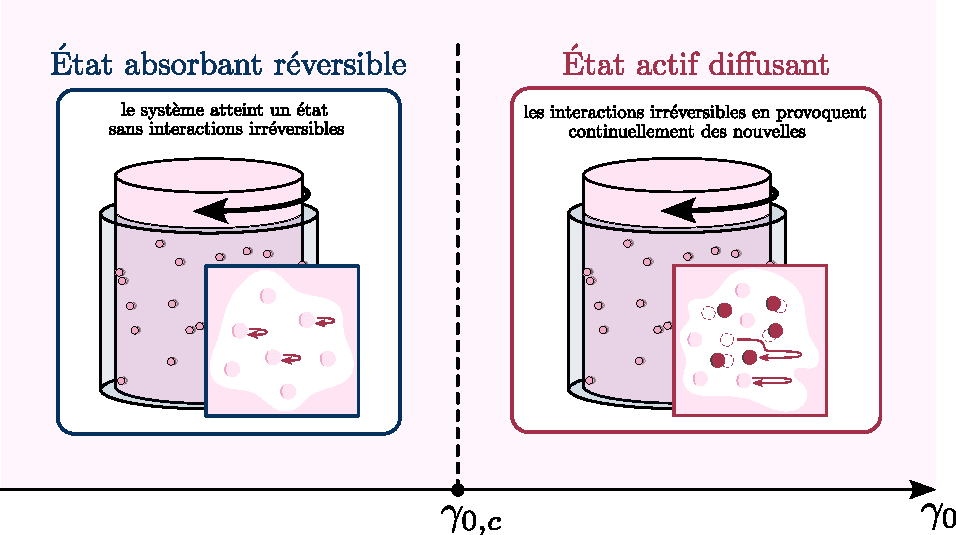
\includegraphics[width=\textwidth]{Chapitre1/Figures/InterpretationCDP/SuspensionsAPT.pdf}
	\caption{Interprétation de la dynamique de la transition de réversibilité comme celle d'une transition de phase absorbante.}
	\label{fig:SuspCDP}
\end{figure}

\subparagraph{}Il y a alors deux possibilités. Dans le premier cas, l'amplitude de cisaillement est suffisamment grande ($\gamma_0 > \gamma_{0,c}$) et la propagation des interactions irréversibles perdure à temps long dans le système, amenant à un coefficient de diffusion stroboscopique non-nul $D_0 >0$. Dans le second cas, l'amplitude de cisaillement globale est trop faible ($\gamma_0 < \gamma_{0,c}$) et le système finit par tomber dans un état réversible où chaque particule suit une orbite stable isolée, amenant à un état stroboscopiquement arrêté $D_0 = 0$.

\subparagraph{}Comme illustré à la \autoref{fig:SuspCDP}, la transition de réversibilité peut donc être comprise comme une transition de phase absorbante dont le paramètre de contrôle est l'amplitude de cisaillement $\gamma_0$ et le paramètre d'ordre le coefficient de diffusion stroboscopique $D_0$. Dans ce système, l'activité est donc directement associée aux déplacements irréversibles des particules, susceptibles de disparaître (via le repositionnement sur une nouvelle orbite stable) ou de se propager (via le repositionnement sur une orbite recoupant une orbite stable), de la même manière que l'activité dans les modèles présentés précédemment. De plus, l'état arrêté dans lequel toutes les particules sont sur une orbite stable est bien un état absorbant puisque la déstabilisation de l'orbite d'une particule ne peut se faire que par l'intersection avec une autre orbite. Ainsi, si toutes les orbites sont stables, elles le resteront pour toujours. Nous pouvons alors définir les mêmes exposants critiques que dans n'importe quelle autre transition de phase absorbante :

\begin{equation}
	D_0 \sim \delta\gamma_0^\beta, \quad \langle \delta D_0^2 \rangle \sim \delta\gamma_0^{-\gamma^\prime},\quad \xi \sim \delta\gamma_0^{-\nu_\perp}, \quad \delta\gamma_0 = \frac{\gamma_0-\gamma_{0,c}}{\gamma_{0,c}}.
\end{equation}

\noindent L'enjeu est alors de connaître la valeur de ces exposants caractérisant cette criticalité.

\subsubsection{Similitudes avec la classe CDP}

\subparagraph{}La classe d'universalité pressentie au premier abord pour la transition de réversibilité est la classe CDP. En effet, nous retrouvons ici un couplage de la propagation de l'activité à celle de la dynamique d'un champ conservé. De fait, les particules, vecteurs de cette propagation dans l'espace, constituent un champ de densité qui, par conservation du nombre de particules (système fermé) est lui-même conservé. De plus, ce système possède un nombre infini d'états absorbants. En effet, tout ensemble d'orbite stable, et il en existe une infinité en espace continu, est un état absorbant. Ainsi, les deux principaux critères de la conjecture de Rossi et. al \cite{rossi_universality_2000} sont respectés. On pourrait donc s'attendre à ce que l'universalité CDP représente cette transition.

\subparagraph{}Afin d'étudier la criticalité de ce système, une approche de modélisation numérique simple a été développée. Celle-ci se concentre uniquement sur la dynamique strobsoscopique du système. Dans ce cadre, comme nous l'expliquerons plus en détail dans le \autoref{chapter:Susp}, le modèle numérique adéquat pour caractériser la transition correspond au ROM que nous avons présenté dans la section précédente. De ce fait, sous cet angle de modélisation, la transition de réversibilité appartient à la classe CDP. Ainsi, en 2D, elle est caractérisée par les exposants critiques $\beta \approx 0.64$ et $\gamma^\prime \approx 0.37$.

\subparagraph{}Toutefois, de notre point de vue, un mécanisme essentiel est perdu dans la simplification de cette modélisation : seules les interactions irréversibles de contact sont prises en compte dans la dynamique du système. Or, dans un système réel, les particules n'interagissent pas seulement par contact direct mais aussi indirectement via le fluide suspendant. Cette simplification est tout sauf anodine puisque, comme nous le discutons dans la partie suivante, la forme pressentie de ces interactions hydrodynamiques est à longue portée. Ceci suggère alors que leur prise en compte est susceptible de modifier significativement la criticalité du système.

\subsubsection{Interactions visqueuses médiées par le fluide}

\label{sec:ref_interac_visc}

\subparagraph{}Dans cette partie nous expliquons brièvement pourquoi nous pensons que le fluide suspendant permet la médiation d'interactions à longue portée entre les particules dans le cadre de la transition de réversibilité, quel que soit le dispositif expérimental considéré. Le raisonnement détaillé est présenté dans l'\annexeref{sec:Annexe_Interactions_Hydro}, nous en présentons simplement ici les conclusions générales dans un souci de concision. Dans le cas de la transition de réversibilité, lorsqu'une particule interagit irréversiblement avec une autre particule au cours d'un cycle, elle quitte son orbite initiale en appliquant une certaine force sur le fluide. Cette force va alors modifier l'écoulement du fluide via les lois régissant sa dynamique et donc affecter le mouvement des particules environnantes. En milieu infini, dans la limite de champ lointain, la force $\mathbf{F}^1(\mathbf{r})=\mathbf{F}^1\delta(\mathbf{r})$ appliquée en $\mathbf{r}$ par une particule $1$ ayant interagi irréversiblement induit une vitesse $\mathbf{v}^2$ sur une particule $2$ située en $\mathbf{r}^\prime$ via la relation linéaire :

\begin{equation}
	v_i (\mathbf{r}^\prime) = \mathcal{G}_{ij}(\mathbf{r} -\mathbf{r}^\prime)F^1_j, \quad \mathcal{G}_{ij}(\mathbf{r}) = \frac{1}{8\pi\eta r}\left( \delta_{ij}+\frac{r_ir_j}{r^2} \right),
\end{equation}

\noindent avec $\mathcal{G}_{ij}$ le tenseur d'Oseen, fonction de Green des équations de Stokes. En pratique cependant, les évènements irréversibles correspondent plutôt à un dipôle de force sur le fluide, représentant le choc des deux particules interagissant. Ainsi, le propagateur d'interaction d'intérêt est plutôt la dérivée de ce tenseur d'Oseen (voir \annexeref{sec:Annexe_Interactions_Hydro}). Celui-ci définit donc une interaction hydrodynamique entre l'évènement irréversibile et les particules environnantes décroissant comme $\sim 1/r^2$ dans le milieu tridimensionnel infini, modélisation adéquate pour décrire le cisaillement de suspensions dans des dispositifs peu confinants.

\subparagraph{}En fait, en se basant sur les principes de conservation de la quantité de mouvement et/ou de la masse dans le système, nous pouvons montrer que dans la grande majorité des dispositifs expérimentaux pertinents pour l'étude de la transition, la forme de l'interaction induite par un monopôle de force reste la même, décrite par :

\begin{equation}
\quad \mathcal{G}_{ij}(\mathbf{r}) \sim \frac{1}{r^\gamma}\left( \delta_{ij}+ C\frac{r_ir_j}{r^2} \right),
\end{equation}

\noindent avec $\gamma$ un entier dépendant du dispositif \cite{diamant_hydrodynamic_2009}. L'interaction entre un évènement irréversible (dipôle de force) et une particule dans la transition de réversibilité décroît donc aussi en loi de puissance comme $\sim 1/r^\alpha$ avec $\alpha = \gamma+1$. Par exemple dans le cas d'un confinement quasi-2D entre deux plaques rigides nous obtenons une décroissance en $\sim 1/r^3$ soit $\alpha = 3$.

\subparagraph{}De manière toute à fait générale, le fluide suspendant permet donc de médier des interactions à longue portée entre les particules. Cette caractéristique n'est pas anodine puisque la conjecture de Rossi et al. \cite{rossi_universality_2000} quant à l'appartenance à la classe CDP suppose implicitement la présence d'interactions à courte portée seulement. La présence d'interactions médiées par le fluide, a priori inévitable, constitue donc un mécanisme de la transition de réversibilité susceptible de rendre sa criticalité différente de celle de la classe CDP. Ce que nous montrons dans la partie suivante est que c'est aussi le cas de la transition vers l'écoulement.

\subsection{Transition vers l'écoulement}

\label{sec:yieldingCDP}

\subparagraph{}En première partie de ce chapitre, nous avons présenté la transition vers l'écoulement des fluides à seuil comme séparant un état coulant d'un état élastique. Pour comprendre plus spécifiquement comment celle-ci peut être appréhendée comme une transition de phase absorbante, il est important de comprendre comment l'écoulement prend place dans la phase active.

\subsubsection{L'écoulement comme une succession de réarrangements}

\subparagraph{}Prenons l'exemple d'un matériau amorphe, comme une mousse, soumis à un cisaillement simple. Lorsque l'on applique une certaine contrainte de cisaillement $\Sigma$ à ce système, celle-ci se voit supportée par les différentes régions du matériau sous forme de contrainte locale $\sigma$. Dans la limite où cette contrainte locale est suffisamment faible, la région associée la supporte en opérant une déformation élastique. Cependant, dès lors que cette contrainte locale dépasse un certain seuil $\sigma_Y$, propre à chaque région, la région associée se déforme plastiquement et irréversiblement. Cette déformation plastique permet alors de relaxer la trop forte contrainte locale et, par conservation de la contrainte appliquée, de la redistribuer aux autres régions du matériau \cite{nicolas_deformation_2018}. 

\subparagraph{}Dans le cas des mousses, les réarrangements plastiques permettant la relaxation de la contrainte locale prennent une forme bien spécifique : les évènements dits T1 \cite{princen_rheology_1986}. Au cours d'un tel évènement, un groupe de quatre bulles (correspondant à une région locale précédemment mentionnée) opère un changement topologique par changement de voisins. Ce processus géométrique de relaxation local de la contrainte est illustré à la \autoref{fig:yieldingchapo}-(a) via les images tirées de \cite{dollet_rheology_2014}. Ce type de réarrangement plastique caractéristique est retrouvé dans l'écoulement d'autres systèmes amorphes comme les émulsions ou les verres métalliques, impliquant dans ce cas un plus grand nombre d'entités microscopiques \cite{nicolas_deformation_2018}. 

\subparagraph{}En redistribuant la contrainte locale relaxée, une région se réarrangeant plastiquement est capable d'induire le dépassement du seuil de contrainte local dans une autre région du matériau. Celle-ci va alors à son tour se réarranger plastiquement, redistribuer son surplus de contrainte locale et déclencher de nouveaux évènements dans le système. Mises à la suite les unes des autres, ces déformations plastiques locales créent alors un écoulement plastique macroscopique global via une dynamique collective.

\subparagraph{}Il y a alors deux possibilités. Dans le premier cas, la contrainte globale appliquée au système $\Sigma$ est trop faible ($\Sigma<\Sigma_c$) et le système finit par tomber dans un état où toutes les régions du matériau sont capables de soutenir la contrainte locale élastiquement ($\sigma < \sigma_Y$). Le matériau ne coule donc pas, on observe un taux de cisaillement nul $\dot{\gamma} = 0$. Dans le second cas, la contrainte globale est suffisamment grande ($\Sigma>\Sigma_c$) pour que, à temps long, le système soit toujours traversé par des réarrangements plastiques locaux. Dans l'état stationnaire, le matériau s'écoule et on mesure un taux de cisaillement non-nul $\dot{\gamma}>0$. Il est important de noter que la dynamique collective complexe à l’œuvre fait que la contrainte seuil globale $\Sigma_c$ ne peut pas être trivialement déduite des contraintes seuil locales $\sigma_Y$.

\begin{figure}[h]
	\centering
	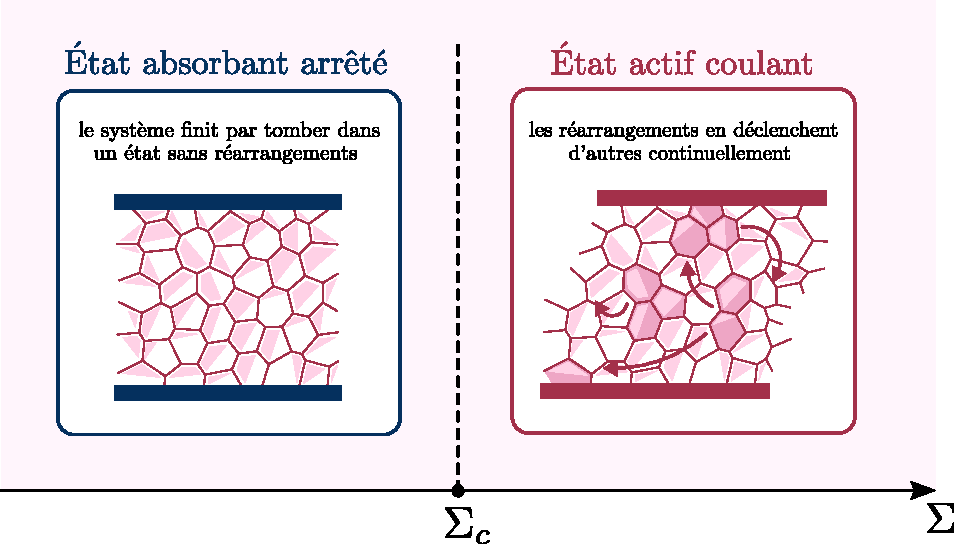
\includegraphics[width=\textwidth]{Chapitre1/Figures/InterpretationCDP/YieldingAPT.pdf}
	\caption{Interprétation de la dynamique de l'écoulement des fluides à seuil comme celle d'une transition de phase absorbante.}
	\label{fig:YieldingCDP}
\end{figure}

\subparagraph{}Comme illustré à la \autoref{fig:YieldingCDP}, la transition vers l'écoulement peut donc être comprise comme une transition de phase absorbante dont le paramètre de contrôle est la contrainte de cisaillement $\Sigma$ et le paramètre d'ordre le taux de cisaillement $\dot{\gamma}$. Dans ce système, l'activité est donc directement associée à la déformation plastique locale du matériau qui est susceptible de s'estomper (via la relaxation de la contrainte locale) comme de se propager (via la redistribution de contrainte), de la même façon que dans les modèles précédemment évoqués dans ce chapitre. Par ailleurs, l'état arrêté représenté par $\dot{\gamma} = 0$ est bien un état absorbant de la dynamique puisque, à $\Sigma$ fixée, un réarrangement plastique ne peut être provoqué que par la redistribution de contrainte engendrée par un réarrangement précédent. De cette façon, on peut définir les mêmes exposants critiques que dans le cadre de n'importe quelle autre transition de phase absorbante :

\begin{equation}
	\dot{\gamma} \sim \delta\Sigma^\beta,\quad \langle\Delta\dot{\gamma}^2\rangle \sim \delta\Sigma^{-\gamma^\prime}, \quad \xi \sim \delta\Sigma^{-\nu_\perp}, \quad \delta\Sigma = \frac{\Sigma-\Sigma_c}{\Sigma_c}.
\end{equation}

\subparagraph{}Il ne va pas sans remarquer que la phénoménologie décrite de la transition vers l'écoulement ressemble fortement à celle de la transition de dépiégeage. On peut en effet faire une analogie directe entre la contrainte globale de cisaillement $\Sigma$ et la force extérieure $f$ de la transition de dépiégeage, et entre le taux de cisaillement $\dot{\gamma}$ et la vitesse de l'interface $v$ dans la transition de dépiégeage. D'ailleurs, plusieurs études se sont concentrées sur la comparaison de ces deux phénomènes \cite{lin_scaling_2014, ferrero_elastic_2019, tyukodi_depinning_2016}. Dans cette optique, on pourrait s'attendre naturellement à ce que la transition vers l'écoulement soit aussi représentée par la classe CDP.

\subsubsection{Similitudes avec la classe CDP}

\subparagraph{}La transition vers l'écoulement semble en effet réunir la plupart des conditions pour l'appartenance à l'universalité CDP. De fait, celle-ci présente une dynamique d'activité couplée à celle d'un champ conservé non-diffusif : le champ de contrainte locale. Par ailleurs, cette transition possède une infinité d'états absorbants. En effet, n'importe quel état du système possédant un champ de contrainte local vérifiant $\sigma < \sigma_Y$ en tout point du matériau est un état absorbant. Les deux critères de la conjecture de Rossi et al. \cite{rossi_universality_2000} sont donc bien vérifiés.

\subparagraph{}Cependant, comme pour la transition de réversibilité, la transition vers l'écoulement fait intervenir des interactions à longue portée, contredisant la condition de courte portée implicitement inscrite dans la conjecture de Rossi et al \cite{rossi_universality_2000}. En effet, nous montrons dans la partie suivante que le milieu élastique dans lequel prennent place les réarrangements plastiques permet de redistribuer la contrainte relaxée à longue portée.

\subsubsection{Interactions élastiques médiées par le solide}

\label{sec:ref_interac_elast}

\subparagraph{}L'effet d'un réarrangement plastique sur le milieu peut être compris dans le cadre de l'élasticité linéaire. Dans cette partie, nous présentons les conclusions du raisonnement mené dans l'\annexeref{sec:Annexe_Eshelby}, permettant de déterminer la modification de contrainte induite par un réarrangement plastique dans le système. Dans un matériau élastique isotrope et incompressible de module de cisaillement $\mu$, une déformation plastique représentée par le tenseur $\epsilon_{ij}^\text{pl}(\mathbf{r})$ entraîne une modification du tenseur des contraintes $\sigma_{ij}(\mathbf{r})$ décrite par la relation linéaire :

\begin{equation}
	\sigma_{ij}(\mathbf{r}) = \int\mathrm{d}\mathbf{r}^\prime~ \mathcal{G}_{ijkl}(\mathbf{r}-\mathbf{r}^\prime)\epsilon^\text{pl}_{kl}(\mathbf{r}^\prime),
\end{equation}

\noindent avec $\mathcal{G}_{ijkl}$ un propagateur dont la forme générale est donnée en annexe.

\subparagraph{}Afin d'obtenir une expression de la modification du champ de contrainte suite à un réarrangement plastique, nous faisons l'hypothèse que celui-ci possède la même symétrie que le forçage, que nous prenons comme un cisaillement simple dans la direction $\hat{\mathbf{e}}_x$. En considérant l'évènement comme ayant lieu en $\mathbf{r}^\prime = 0$, on a alors en 2D : $\epsilon_{xy}^\text{pl}(\mathbf{r}^\prime) = \epsilon_{yx}^\text{pl}(\mathbf{r}^\prime) = \epsilon^\text{pl}\delta(\mathbf{r}^\prime)$ et $\epsilon_{xx}^\text{pl}(\mathbf{r}^\prime) = \epsilon_{yy}^\text{pl}(\mathbf{r}^\prime) = 0$. Via cette modélisation, la modification de la contrainte locale de cisaillement\footnote{Des expressions similaires peuvent être obtenues pour les composantes $\sigma_{xx}$ et $\sigma_{yy}$ du tenseur des contraintes. Toutefois, on se concentrera ici seulement sur la contrainte locale de cisaillement $\sigma_{xy}$.} dans le matériau est donnée par :

\begin{equation}
	\sigma_{xy}(\mathbf{r})= \sigma_{yx}(\mathbf{r}) = 2\mu \mathcal{G}(\mathbf{r}) \epsilon^\text{pl}, \quad \mathcal{G}(\mathbf{r}) = \frac{\cos (4\theta)}{\pi r^2}.
	\label{eq:Eshelby}
\end{equation}

\subparagraph{}On appelle alors le propagateur $\mathcal{G}$ propagateur d'Eshelby\footnote{Sa dénomination revient à la personne l'ayant calculé en premier \cite{eshelby_determination_1997}.}, dont la forme correspond à la modification de contrainte à l'issue d'un unique réarrangement plastique localisé. La redistribution de contrainte opérée lors d'un tel évènement est donc effectivement à longue portée, décroissant comme $\sim 1/r^2$ en 2D.

\paragraph{Forme et observations expérimentales}

\subparagraph{}Sur la \autoref{fig:EshelbyExp}-(a), nous représentons la redistribution de la contrainte de cisaillement locale suite à un réarrangement plastique. Comme on peut le remarquer, en plus d'être à longue portée, la redistribution est fortement anisotrope. Plus particulièrement, le signe de celle-ci dépend de la direction considérée : la redistribution est positive dans les directions principales du cisaillement $\hat{\mathbf{e}}_x$ et $\hat{\mathbf{e}}_y$ et négative dans les directions intermédiaires. En d'autres termes, un réarrangement plastique d'une région dans le milieu élastique déstabilise aussi bien qu'il ne stabilise les autres régions. Par ce mécanisme, la plasticité dans le milieu favorise donc la propagation de l'activité en même temps qu'elle l'inhibe (une redistribution de contrainte négative défavorise le déclenchement d'un nouveau réarrangement plastique).

\begin{figure}[h]
	\centering
	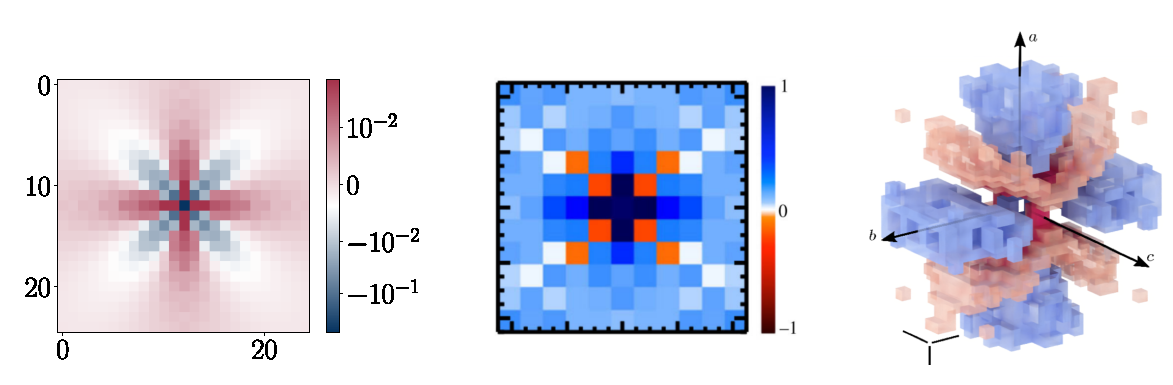
\includegraphics[width=\textwidth]{Chapitre1/Figures/InterpretationCDP/EshelbyExp.pdf}
	\caption{Anisotropie de la redistribution de contrainte après un réarrangement plastique (les unités spécifiques n'ont pas d'importance). (a) Représentation en 2D du propagateur d'Eshelby défini par l'\autoref{eq:Eshelby}. (b) Redistribution de contrainte suite à un réarrangement plastique mesurée dans \cite{desmond_measurement_2015}. (c) Idem dans \cite{schott_multiscale_2024}, les zones rouges représentent des redistributions positives et les zones bleues des redistributions négatives.}
	\label{fig:EshelbyExp}
\end{figure}

\subparagraph{}La redistribution de la contrainte suite à un tel évènement a été mesurée en conditions réelles dans différents systèmes, confirmant la forme prédite par la théorie continue \cite{desmond_measurement_2015, schott_multiscale_2024, jensen_local_2014}. Par exemple, dans \cite{schott_multiscale_2024}, les auteurs ont mesuré la redistribution de contrainte dans une mousse après un évènement T1 et ont pu mettre en évidence la forme quadrupolaire caractéristique du propagateur d'Eshelby. D'autre part, via des simulations de dynamique moléculaire, la topologie et la portée de l'interaction d'Eshelby s'est aussi vue confirmée dans différents systèmes \cite{kabla_local_2003, maloney_amorphous_2006, tanguy_plastic_2006}. Cette forme simple de l'interaction permet alors d'encoder le mécanisme d'écoulement des fluides à seuil dans des modèles mésoscopiques que nous présenterons au \autoref{chapter:yielding}.

\subparagraph{}De la même façon que dans le cas des suspensions, les dispositifs expérimentaux étudiés peuvent agir significativement sur la portée des interactions. Si l'on considère par exemple un écoulement quasi-2D entre deux plaques rigides, celui-ci implique une redistribution de contrainte suite à un évènement plastique décroissant comme $\sim 1/r^4$ à grande distance (voir \autoref{sec:lambda_picard}). Ainsi, comme dans le cas des suspensions, le caractère de longue portée des interactions médiées est génériquement présent.

\subparagraph{}In fine, il semble donc aussi que la transition vers l'écoulement des fluides à seuil peut être comprise dans le cadre CDP avec la présence additionnelle d'interactions à longue portée.

\section{Atypicité des transitions étudiées}

\subparagraph{}D'après les éléments soulevés dans la section précédente, les transitions de réversibilité et d'écoulement semblent correspondre au cadre de description CDP en présence d'interactions à longue portée. Dans le cadre d'étude des transitions de phase continues, l'influence des interactions à longue portée sur le comportement critique peut être compris dans un cadre générique. Dans cette section, nous montrons via des mesures pré-existantes que les transitions que nous proposons d'étudier dans cet ouvrage ne peuvent en fait pas être rapportées à ce cadre. Nous proposons alors une explication à cette divergence via la nature des interactions qu'elles mettent en place. Celles-ci définissent en effet un mécanisme de propagation de l'activité original, échappant au cadre théorique habituel.

\subsection{Incompatibilité avec le cadre générique de la longue portée}

\subsubsection{Attendu générique de l'influence d'interactions à longue portée}

\subparagraph{}Dans un système présentant des interactions à longue portée, décroissant comme ${\sim 1/r^\alpha}$, tous les agents microscopiques sont liés. Ce lien est d'autant plus fort que la portée de l'interaction est grande (i.e. $\alpha$ petit). Dans la limite où cette portée est infinie, tous les agents interagissent de manière équivalente entre eux, détruisant ainsi la notion d'espace dans le système. De ce fait, son comportement équivaut à celui du champ moyen associé. \`A l'opposé de ce spectre, dans la limite où cette portée est infiniment faible, l'interaction non-locale n'est significative que dans le voisinage direct de chaque agent. Ainsi, ce cas se rapporte à la présence d'interactions locales uniquement.

\subparagraph{}Cette phénoménologie trouve écho dans les phénomènes critiques. Lorsque l'on généralise l'interaction locale sous-jacente d'un phénomène critique au cas de longue portée, décrit par un exposant $\alpha$, le comportement critique présente deux cas limites. Dans la limite de grande portée, le comportement critique retrouvé est celui du champ moyen, décrit par des exposants critiques triviaux. \`A l'inverse, dans la limite de courte portée, les exposants critiques décrivant le système prennent leur valeur non-triviale de dimension finie. Dans un système présentant des interactions caractérisées par un exposant $\alpha$ arbitraire, on s'attendra donc à trouver une criticalité encadrée par son équivalent de courte portée et le champ moyen associé.

\subparagraph{}Par exemple, dans le cas de nos deux transitions d'intérêt, la classe a priori adéquate pour décrire le comportement à courte portée est la classe CDP. Ainsi, avec la présence additionnelle d'interactions à longue portée, on peut s'attendre à mesurer des exposants critiques compris entre ceux donnés par la criticalité CDP en dimension finie et ceux donnés par la criticalité CDP en champ moyen. D'après les valeurs connues de ces deux limites que nous avons répertoriées au \autoref{tab:expocrit_DPCDP}, on s'attendrait par exemple à mesurer en 2D un exposant $\beta$ encadré comme $0.64 < \beta < 1$ et un exposant $\gamma^\prime$ encadré comme $0 < \gamma^\prime < 0.37$.

\subparagraph{}Dans la partie suivante, nous montrons que les mesures réalisées précédemment sur des systèmes représentant ces transitions contredisent cette attente naturelle.

\subsubsection{Contradiction du cadre générique par les transitions de réversibilité et d'écoulement}

\paragraph{Transition de réversibilité}

\subparagraph{}Dans une étude menée par Mari et. al \cite{mari_absorbing_2022}, les auteurs ont proposé de pallier à l'absence des interactions hydrodynamiques dans les simulations numériques stroboscopiques pré-existantes. Pour ce faire, en reprenant le cadre de modélisation offert par le ROM, les auteurs ont explicitement intégré l'effet de ces interactions en les représentant par une diffusion effective des particules. Celle-ci est décrite par un coefficient de diffusion proportionnel au nombre de particules actives (i.e. subissant une interaction de contact irréversible à un instant $t$) dans le système. Cela équivaut alors en quelque sorte à considérer les interactions médiées dans une approche de champ moyen, c'est-à-dire de portée infinie\footnote{La philosophie derrière cette modélisation sera présentée plus en détail au \autoref{chapter:Susp}.} ($\alpha = 0$). 

\subparagraph{}Ce faisant, les auteurs ont étudié le comportement critique du système en 2D et mesuré les exposants critiques $\beta$ et $\gamma^\prime$ associés, trouvant les valeurs :

\begin{equation}
	\beta \approx 1.85 \quad \gamma^\prime \approx -1.2.
\end{equation}

\noindent Ces valeurs sont alors en contradiction avec l'effet générique des interactions à longue portée sur la classe CDP, puisqu'elles ne sont pas encadrées par les limites de champ moyen et de courte portée associées. Notamment, elles décrivent une évolution convexe du paramètre d'ordre avec la distance au point critique ($\beta >1$), là où la criticalité CDP généralisée au cas d'interactions à longue portée décrit une évolution concave, voire linéaire ($\beta = 1$). Même si l'implémentation de ces interactions peut être discutée (dans un système réel, nous avons montré que leur portée était caractérisée par $\alpha > 0$), leur intégration dans le modèle semble exclure la transition de l'attendu générique.


\begin{figure}[h]
	\centering
	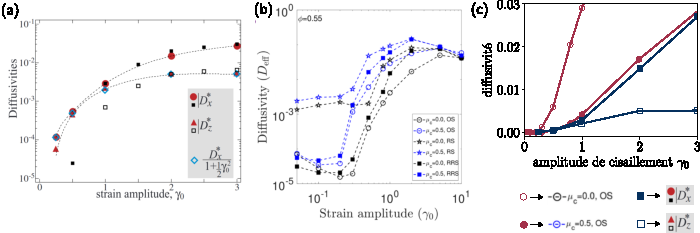
\includegraphics[width=\textwidth]{Chapitre1/Figures/LongRange/ExpShear.pdf}
	\caption{Caractérisation de la transition de réversibilité dans les suspensions cisaillées cycliquement dans des études de dynamique moléculaire. Évolution de la diffusivité stroboscopique avec l'amplitude de cisaillement dans l'étude \cite{metzger_irreversibility_2010} (a) et \cite{agrawal_dense_2024} (b). (c) Représentation lin-lin de certaines courbes tirées de (a) et (b), spécifiées dans la légende.}
	\label{fig:ShearedExp}
\end{figure}

\subparagraph{}Si l'on regarde du côté des expériences (voir \autoref{fig:suspchapo}-(b)) ou des simulations plus réalistes de dynamique moléculaire, les mesures proposées sur ces systèmes ne semblent par ailleurs pas vraiment contredire cette observation. En effet, sur la \autoref{fig:ShearedExp}-(c) où nous avons reproduit les résultats des études \cite{metzger_irreversibility_2010, agrawal_dense_2024}, il n'apparaît pas clairement que l'évolution du paramètre d'ordre soit concave et semble même convexe. 

\subparagraph{}Ces éléments suggèrent alors que la transition de réversibilité pourrait ne pas être appréhendée via l'extension à longue portée générique de la classe CDP. Dans la sous-section suivante, nous montrons qu'il en est de même pour la transition vers l'écoulement.

\paragraph{Transition vers l'écoulement}

\subparagraph{}La criticalité de la transition vers l'écoulement a été déjà étudiée via des modèles mésoscopiques numériques en deux dimensions que nous présenterons au \autoref{chapter:yielding}\cite{lin_scaling_2014, liu_driving_2016, ferrero_criticality_2019, picard_slow_2005}. Dans les travaux associés, l'exposant $\beta$ a été mesuré à plusieurs reprises comme $\beta\approx 1.5$, montrant ainsi à nouveau une évolution convexe du paramètre d'ordre avec la distance au point critique.

\subparagraph{}Ces mesures sont en accord qualitatif avec de nombreuses expériences réalisées sur les fluides à seuil. Dans ce domaine d'étude, il est d'usage de modéliser la courbe d'écoulement $\dot{\gamma} = f(\Sigma)$ du système par la loi d'Herschel-Bulkley :

\begin{equation}
	\Sigma = \Sigma_c + k\dot{\gamma}^n, \quad k > 0,
\end{equation}

\noindent avec $n$ l'exposant d'Hershel-Bulkley, directement associé à l'exposant $\beta$ des phénomènes critiques via $n=1/\beta$. De nombreux travaux, menés sur différents systèmes amorphes, ont déterminé des exposants $n<1$ soit $\beta > 1$, correspondant à une transition vers l'écoulement convexe, comme dans le cas des modèles mésoscopiques \cite{nicolas_deformation_2018}.

\subparagraph{}Ces éléments suggèrent donc que la transition vers l'écoulement, comme la transition de réversibilité, ne correspond pas à l'attente naturelle de l'extension à longue portée de la classe CDP. De ce point de vue, ces deux transitions présentent un point commun très fort, qui motive leur étude simultanée. Cette étude est en fait d'autant plus intéressante qu'un indice apparent semble par ailleurs rapprocher ces deux transitions tout en les éloignant du cadre générique : dans ces deux systèmes, les interactions à longue portée induisent un mécanisme de propagation de l'activité original.

\subsection{Des interactions à longue portée de nature différente}

\subsubsection{La longue portée comme transport dans le cadre d'interprétation générique}

\subparagraph{}En fait, comme nous le détaillerons dans le \autoref{chapter:TransportLP}, dans le cadre générique d'évolution de la criticalité CDP avec les interactions à longue portée, celles-ci sont représentées par un transport à longue portée de la quantité conservée induit localement par l'activité.

\subparagraph{}Dans le cadre des modèles de particules comme le modèle Manna ou le ROM, cela revient à considérer que les particules actives font des sauts $\mathbf{r}^\prime$ distribués selon $P(\mathbf{r}^\prime)\sim 1/|\mathbf{r}^{\prime}|^{\alpha}$, et non plus uniquement dans leur voisinage direct. Dans cette approche, les interactions à longue portée représentent donc un transport de masse à longue portée induit localement par l'activité.

\subparagraph{}Dans le cas de la transition de dépiégeage, nous avions associé la redistribution de masse à la redistribution de force élastique. Ainsi, l'extension à longue portée de ce phénomène correspond dans ce cas à des interactions élastiques à longue portée. Le propagateur qui redistribue cette force élastique est alors le pendant direct de la distribution de probabilité des sauts dans les modèles de particules. On peut donc voir dans la transition de dépiégeage à longue portée un transport de la force élastique à longue portée induit localement par l'activité. C'est en fait un cas d'étude qui a concentré de nombreux travaux car certains problèmes de dépiégeage présentent de l'élasticité à longue portée (voir \annexeref{app:exp_depinning}).


\subparagraph{}Ce que nous montrons dans cette sous-section, c'est que les interactions à longue portée médiées par le milieu dans les transitions de réversibilité et d'écoulement ne peuvent pas vraiment être comprises comme un transport à longue portée de la quantité conservée induit localement par l'activité, ou en tous cas pas complètement.

\begin{figure}[h]
	\centering
	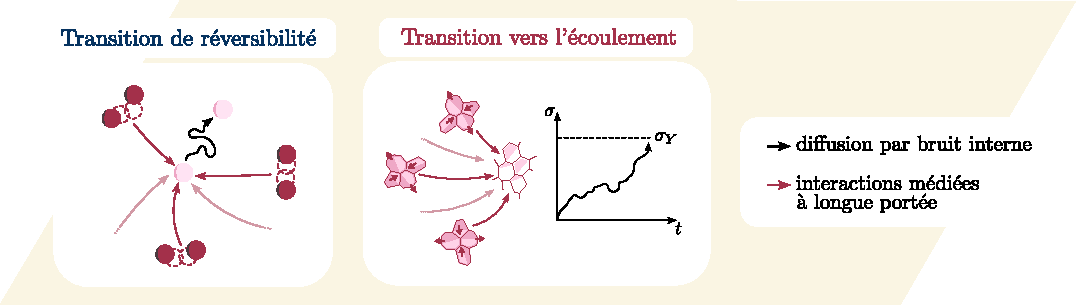
\includegraphics[width=\textwidth]{Chapitre1/Figures/Pb/bruit.pdf}
	\caption{Nouveaux mécanismes de création d'activité induits par les interactions à longue portée dans la transition de réversibilité et la transition vers l'écoulement.}
	\label{fig:bruit}
\end{figure}

\subsubsection{La longue portée comme source de diffusion dans les transitions de réversibilité et d'écoulement}

\paragraph{Transition de réversibilité}

\subparagraph{}Dans le cas de la transition de réversibilité, les interactions hydrodynamiques provoquent des petits déplacements des particules dans tout le milieu suite à un évènement irréversible. Ainsi, ce n'est pas la particule à l'origine de l'interaction irréversible qui est transportée à longue portée, mais plutôt l'influence de l'activité sur les particules qui est à longue portée. Dans ce cas, la longue portée ne prend pas la forme d'un transport mais plutôt d'un bruit interne : chaque particule est soumise à des petits déplacements induits à longue portée par l'activité dans le système. Un nouveau mécanisme potentiel de création d'activité prend place : via l'influence de ce bruit interne, l'orbite stable associée à une particule passive peut se déformer progressivement jusqu'à rencontrer une autre orbite stable et ainsi créer un évènement irréversible. En d'autres termes, la création d'activité peut être approchée par une sorte de diffusion (et non plus par un déplacement fini issu d'un évènement irréversible précédent) induite de manière non-locale.

\paragraph{Transition vers l'écoulement}

\subparagraph{}Comme nous l'avons mentionné à la \autoref{sec:yieldingCDP}, la transition vers l'écoulement est très proche de celle du dépiégeage. De la même façon que l'on peut voir la redistribution de force élastique dans le dépiégeage comme un transport induit localement par l'activité, on peut appréhender une partie de la redistribution de contrainte dans la transition vers l'écoulement comme tel. Lors du réarrangement plastique d'une région, la contrainte locale de celle-ci est relaxée et transmise aux autres régions du matériau. Toutefois, l'effet complet de la redistribution ne peut pas être appréhendé comme tel. En effet, comme nous l'avons mentionné à la \autoref{sec:yieldingCDP}, le propagateur d'Eshelby est de signe alterné. Ainsi, à la différence du propagateur élastique associé au dépiégeage qui est toujours positif, il ne peut pas être le pendant direct de la distribution de probabilité associée au transport de masse dans les modèles de particules. \`A la place, la propriété de signe alterné montre qu'une partie de l'interaction peut être comprise comme un bruit mécanique, qui peut autant stabiliser que déstabiliser une région du matériau. Cette interprétation n'est d'ailleurs pas nouvelle dans le cadre de cette transition \cite{lin_mean_field_2016, ferrero_criticality_2019}. Ainsi, en plus du mécanisme de transport induit localement par l'activité qui tend à déstabiliser globalement le matériau, un mécanisme de diffusion induite non-localement des contraintes locales vers les contraintes seuils locales prend place (voir \autoref{fig:bruit}). De la même manière que dans la transition de réversibilité, on a donc un mécanisme de création de l'activité par diffusion induite de manière non-locale.

\subparagraph{}Finalement, dans ces deux transitions présentant un comportement critique non conventionnel, nous retrouvons un mécanisme de création de l'activité par diffusion issu des interactions à longue portée. Nous pensons alors que c'est ce mécanisme qui permet d'expliquer les spécificités associées à la transition de réversibilité dans les suspensions cisaillées cycliquement et à la transition vers l'écoulement des fluides à seuil, en contradiction avec l'attente naturelle de l'effet d'interactions à longue portée sur un phénomène critique. \`A partir de ce point plusieurs questions se posent, lesquelles constitueront le fil conducteur de cette thèse.

\section{Problématisation}

\subsection{Questions guidant ce travail}

\paragraph{Quelle criticalité caractérise les transitions de réversibilité et d'écoulement ?}

\subparagraph{}Le premier axe de recherche autour duquel s'articule ce travail correspond à la caractérisation des deux transitions. Nous nous demanderons notamment quelles sont les valeurs prises par les exposants critiques dans le cas d'interactions à longue portée réalistes, i.e. réalisables en conditions expérimentales. Plusieurs questions concernant cette caractérisation découlent de l'étude menée par Mari et al. \cite{mari_absorbing_2022} sur la transition de réversibilité avec portée infinie des interactions médiées par le milieu. 

\subparagraph{}Nous nous demanderons d'abord si les spécificités non-conventionnelles révélées par cette étude sont toujours présentes dans un système présentant une transition de réversibilité avec des interactions décroissant en loi de puissance avec la distance ($\alpha > 0$). Notamment, nous chercherons à savoir si la transition reste dans ce cas convexe ($\beta >1$) et avec des fluctuations qui s'annulent à l'approche du point critique ($\gamma^\prime < 0$) comme observé par Mari et al. \cite{mari_absorbing_2022}. Par ailleurs, dans cette étude de portée infinie, la double non-conventionnalité $\beta >1$ et $\gamma^\prime < 0$ avait été rationalisée par la relation d'hyperscaling $2\beta + \gamma^\prime = \nu_\perp D$, qui justifie une valeur anormalement faible de $\gamma^\prime$ par une valeur anormalement grande de $\beta$. Les caractérisations précédentes de la transition vers l'écoulement révélant un exposant $\beta >1$, nous nous demanderons alors si, vue comme une transition de phase absorbante, celle-ci présente aussi des fluctuations d'activité qui s'annulent à l'approche du point critique.

\subparagraph{}Mari et al. ont par ailleurs montré que la propriété d'hyperunformité était effacée par l'ajout des interactions hydrodynamiques de portée infinie. Nous nous demanderons alors si cette perte d'hyperuniformité est aussi retrouvée dans les cas de portées réalistes de l'interaction. Par analogie, nous transposerons cette question dans le cas de la transition vers l'écoulement : le système présente-t-il une forme d'hyperuniformité en présence des interactions élastiques d'Eshelby à longue portée ?

\subparagraph{}Enfin, nous nous intéresserons à la forme prise par les dynamiques d'avalanche proche du point critique dans ces deux systèmes.

\paragraph{Quelle est l'influence de la portée des interactions médiées sur la criticalité de ces systèmes ?}

\subparagraph{}Dans le \autoref{chapter:TransportLP}, nous présenterons plus en détail le cadre générique d'appréhension des interactions à longue portée, comprises alors comme un transport à longue portée de la quantité conservée induit localement par l'activité, dans un système appartenant à la classe CDP. Celui-ci montre en fait une évolution de la criticalité bien définie en fonction de la valeur de $\alpha$.

\subparagraph{}Or, nous avons montré que les transitions de réversibilité et d'écoulement ne semblent pas pouvoir être décrites dans ce cadre. Dès lors, le rôle de la longue portée des interactions dans ces systèmes n'est pas évident. Nous chercherons à comprendre de manière systématique l'influence de la portée sur les différents aspects de la criticalité de ces systèmes, i.e. à déterminer comment évoluent les exposants critiques caractérisant l'état stationnaire du système, ceux caractérisant son hyperuniformité et ceux caractérisant sa dynamique d'avalanche en fonction de l'exposant de portée $\alpha$.

\subparagraph{}Nous chercherons alors à comparer ces évolutions avec celles du cadre générique, afin de comprendre dans quelle mesure cette nature différente des interactions rend le cadre d'appréhension usuel inadéquat.

\paragraph{Peut-on comprendre ces systèmes similaires dans un cadre de description commun ?}

\subparagraph{}Le troisième axe d'étude consiste à comprendre la transition de réversibilité et d'écoulement dans un cadre commun. Notamment nous nous interrogerons sur la possibilité d'une description champ moyen permettant de rendre compte des observations faites sur les dynamiques en dimension finie, via la prise en compte du nouveau mécanisme de création proposé par les interactions médiées à longue portée. La mise en place de ce cadre pourrait alors aider à mettre en évidence les similarités et les différences éventuelles entre ces deux phénomènes. Aussi, nous nous interrogerons sur la possibilité d'une description continue, à la manière des équations de champ dans la théorie CDP et son extension à longue portée, pour décrire la dynamique de ces systèmes en toute dimension.

\subsection{Déroulé du manuscrit}

\subparagraph{}Pour répondre à toutes les questions révélées par ce chapitre, nous organiserons ce manuscrit comme suit :

\subparagraph{}Dans le \autoref{chapter:TransportLP}, nous caractériserons quantitativement le cadre générique d'appréhension de la longue portée en 2D pour pouvoir mener convenablement, par contraste, l'étude des transitions de réversibilité et d'écoulement dans les chapitres suivants. Pour ce faire, nous généraliserons les modèles Manna et ROM dans le cas d'un transport à longue portée et caractériserons l'évolution des exposants critiques et des propriétés d'hyperuniformité en fonction de la portée de la redistribution de masse. 

\subparagraph{}Dans le \autoref{chapter:Susp}, nous nous concentrerons sur la transition de réversibilité dans les suspensions cisaillées cycliquement. En généralisant le modèle numérique initialement proposé par Mari et al. \cite{mari_absorbing_2022}, nous étudierons la criticalité du système associée à différentes portées des interactions médiées. Cette caractérisation se fera via la détermination des exposants critiques et l'étude des propriétés d'hyperuniformité et des statistiques d'avalanches. Ensuite, nous proposerons un modèle champ moyen permettant de rendre compte des spécificités de la transition via la compréhension du mécanisme de diffusion induit par les interactions médiées à longue portée. Nous comparerons enfin les prédictions de ce modèle avec les résultats obtenus en dimension finie afin de mettre en évidence les sources de complexité dans la dynamique réelle.

\subparagraph{}Dans le \autoref{chapter:yielding}, nous nous concentrerons sur la transition vers l'écoulement des fluides à seuil. Nous proposerons tout d'abord une étude détaillée de la transition en présence d'interactions élastiques d'Eshelby, via l'utilisation d'un modèle mésoscopique numérique. Ensuite, nous mettrons en évidence deux ingrédients susceptibles d'expliquer les spécificités de la criticalité associée : celui déjà évoqué concernant la nature spécifique des interactions à longue portée, et une symétrie particulière retrouvée dans le propagateur de redistribution. Puis, nous procéderons à une généralisation de notre modèle pour étudier différentes portées d'interactions afin de comprendre l'influence de ces dernières sur le comportement critique. Comme pour les modèles précédents, cette caractérisation portera sur l'évolution des exposants critiques, des propriétés d'hyperuniformité et de la dynamique d'avalanche.

\subparagraph{}Enfin, dans un dernier chapitre, nous mettrons face à face les résultats obtenus dans les deux chapitres précédents. Cela nous permettra de tisser une analogie directe entre la transition de réversibilité dans les suspensions cisaillées cycliquement et la transition vers l'écoulement des fluides à seuil. Nous discuterons alors de l'application à la transition vers l'écoulement du cadre théorique présenté au \autoref{chapter:Susp} pour la transition de réversibilité. Cette analyse permettra de souligner les points communs et les différences entre les deux systèmes et d'en fournir une image globale, montrant l'utilité d'une telle étude comparée.
\chapter{Transport à longue portée dans la classe CDP}

\label{chapter:TransportLP}

\subparagraph{}Dans le chapitre précédent, nous avons présenté la classe CDP comme une classe d'universalité recouvrant potentiellement un grand nombre de transitions de phase absorbantes. Un système appartenant à cette classe est décrit par un ensemble de comportements et d'exposants critiques caractéristiques de la criticalité associée. Par exemple, en notant $\langle A \rangle$ l'activité moyenne dans le système, $\langle \delta A^2 \rangle$ ses fluctuations, $\xi$ la longueur de corrélation et $\epsilon$ la distance au point critique, les exposants $\beta$, $\gamma^\prime$ et $\nu_\perp$ permettent de définir les évolutions suivantes proche de la transition :

\begin{equation}
	\langle A \rangle \sim \epsilon^\beta, \quad \langle \delta A^2 \rangle \sim \epsilon^{-\gamma^\prime}, \quad \xi \sim \epsilon^{-\nu_\perp}
\end{equation}

\noindent Ces exposants sont connus exactement dans l'approximation de champ moyen avec $\beta^\text{CM} = 1$, $\gamma^{\prime\text{CM}} = 0$, $\nu_\perp^\text{CM} = \frac{1}{2}$. En dimension finie $D<4$ et en présence d'interactions à courte portée uniquement, les exposants critiques ont été mesurés numériquement \cite{lubeck_universal_2004} et calculés analytiquement, de manière perturbative, via les méthodes du groupe de renormalisation fonctionnel appliquées à la transition de dépiégeage.

\subparagraph{}Comme nous l'avons mentionné au \autoref{chapter:introduction}, la présence d'interactions à longue portée dans les modèles représentant des phénomènes critiques permet en général de passer du comportement critique de dimension finie au comportement critique de champ moyen de la classe d'universalité associée. Dans ce chapitre, nous proposons de définir plus précisément ce cadre générique associé à l'universalité CDP. L'établissement de ce cadre est un objet central dans notre travail puisqu'il nous permettra, par contraste, d'interpréter le comportement atypique des transitions de réversibilité et d'écoulement dans les chapitres suivants.

\subparagraph{}Pour ce faire, nous commencerons par identifier ce cadre, que nous baptisons LR-CDP pour \textit{long-range conserved directed percolation}, d'un point de vue théorique. S'appuyant sur des résultats pré-existants, cette première analyse permettra de définir l'évolution du comportement critique attendue avec la portée des interactions. Nous verrons par ailleurs que, dans ce cadre naturel d'extension de la théorie CDP, les interactions à longue portée représentent un transport à longue portée de la quantité conservé sous l'influence locale de l'activité. Afin de disposer d'un socle de comparaison solide, nous préciserons dans un second temps ce cadre théorique via une approche numérique. Cette caractérisation se fera via l'étude des modèles Manna et ROM et leur extension au cadre LR-CDP en 2D, dimension dans laquelle nous étudierons les transitions de réversibilité et d'écoulement par la suite. Cette analyse sera menée via la détermination des exposants critiques statiques et dynamiques associés et l'évolution des propriétés d'hyperuniformité avec la portée du transport.

\section{Longue portée et comportement critique}

\subparagraph{}Dans cette section, nous présentons le cadre générique de compréhension des interactions à longue portée dans le cas de la criticalité CDP. Après avoir explicité la phénoménologie globale induite par la présence de ce type d'interactions, nous présenterons l'extension naturelle de la théorie CDP via la modification des équations de champ associées. Celle-ci nous permettra alors de déterminer un comportement qualitatif attendu quant à l'évolution de chaque exposant critique avec l'exposant de portée $\alpha$, soutenue par des calculs analytiques pré-existants.

\label{sec:LRCanonique}

\subsection{Phénoménologie}

\subparagraph{}Dans de nombreux systèmes de physique statistique faisant intervenir des transitions de phase, les interactions entre agents prennent un caractère non-local. Dans la plupart de ces cas, cette non-localité peut-être représentée par des interactions décroissant algébriquement avec la distance $r$ séparant les agents, soit comme $\sim 1/r^\alpha$ avec $\alpha >0$. On peut par exemple penser aux interactions de Coulomb entre deux charges ou aux interactions gravitationnelles entre deux masses qui décroissent comme $\sim 1/r$ en trois dimensions, soit $\alpha = 1$. 

\subparagraph{}Comme nous l'avons vu précédemment, dans la limite $\alpha \rightarrow 0$ un système adopte naturellement le comportement critique équivalent au champ moyen de la classe d'universalité associée. \`A l'inverse, dans la limite $\alpha \rightarrow \infty$, ce système adopte le comportement critique de la classe en dimension finie. En fait, dans le cas général, ces deux comportement limites ne prennent pas uniquement place pour des formes asymptotiques de la portée d'interaction. \`A la place, il est possible d'identifier deux bornes $\alpha^+$ et $\alpha^-$ définissant deux zones. Dans toute la gamme d'exposants $\alpha>\alpha^+$, le système présente son comportement critique de courte portée, associé au cas faisant intervenir des interactions locales uniquement. De la même façon, dans toute la gamme d'exposants $\alpha < \alpha^-$, le comportement critique mesuré est celui du champ moyen associé.

\begin{figure}[h]
	\centering
	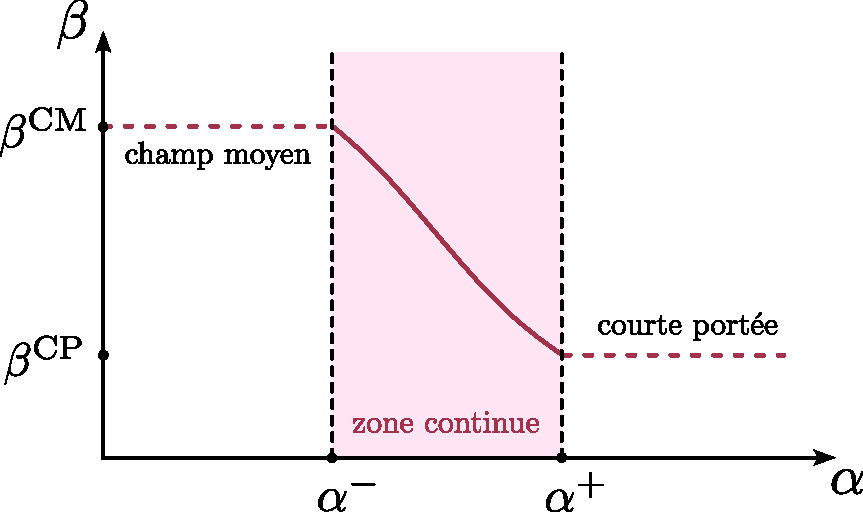
\includegraphics[width=0.7\textwidth]{Chapitre1/Figures/LongRange/beta_base.pdf}
	\caption{Évolution générique de l'exposant $\beta$ avec la portée d'interaction. $\beta^\text{CP}$ est l'exposant attendu dans un modèle avec interactions locales et $\beta^\text{CM}$ est l'exposant attendu dans le cas champ moyen. Cette évolution générique est retrouvée pour les autres exposants critiques.}
	\label{fig:exp_base}
\end{figure}

\subparagraph{}Dans le cas d'une portée intermédiaire $\alpha^- < \alpha < \alpha^+$, plusieurs scénarios sont intuitivement possibles. En fait, ce que l'on observe et rationalise c'est qu'entre ces deux bornes, le comportement critique évolue continûment avec la portée. Chaque exposant critique prend une valeur unique dépendant uniquement de la portée $\alpha$, reliant une valeur de courte portée pour $\alpha = \alpha^+$ à une valeur de champ moyen pour $\alpha = \alpha^-$, comme représenté à la \autoref{fig:exp_base}. Ainsi, il est possible de définir une infinité continue de classes d'universalité associées à celle de courte portée.

\subparagraph{}Cette phénoménologie étant tout à fait générale, retrouvée aussi bien dans les cas d'équilibre que dans les cas hors d'équilibre, nous cherchons à la préciser dans le cas de la classe d'universalité CDP.

\subsection{Formulation théorique dans la classe CDP}

\paragraph{Équations de champ et transport de masse}

\subparagraph{}Il est possible de comprendre la phénoménologie liée à l'ajout d'interactions à longue portée via les théories continues associées aux phénomènes critiques. Généralement, dans le cas de la présence d'interactions à longues portées, les équations de champ sont modifiées par l'ajout de termes d'interactions généralisés. Là où les interactions locales sont représentées par l'opérateur laplacien $\nabla^2$, représenté par un terme en $\sim -q^2$ dans l'espace réciproque, les interactions non-locales sont représentées par l'opérateur de dérivée fractionnaire $|\nabla|^{\alpha-D}$, représenté par un terme en $\sim |q|^{\alpha-D}$ dans l'espace réciproque \cite{hinrichsen_non_equilibrium_2007}. Dans le cas de la théorie de champ CDP, les équations généralisées prennent donc la forme :

\begin{equation}
\begin{aligned}
	&\partial_t A(\mathbf{r}, t) = (\omega\rho (\mathbf{r}, t) - r)A(\mathbf{r}, t) - uA^2(\mathbf{r}, t) + \kappa\nabla^2 A (\mathbf{r}, t) - \kappa_\alpha|\nabla|^{\alpha-D} A (\mathbf{r}, t) + \sigma \sqrt{A(\mathbf{r}, t)} \eta(\mathbf{r}, t)\\
	&\partial_t \rho (\mathbf{r}, t) = \kappa\nabla^2 A (\mathbf{r}, t)- \kappa_\alpha|\nabla|^{\alpha-D} A (\mathbf{r}, t)
\end{aligned}
\label{eq:LRCDP}
\end{equation}

\noindent avec :

\begin{equation}
	|\nabla|^{\alpha-D} A (\mathbf{r}, t) \propto \int \mathrm{d}\mathbf{r}^\prime ~ \frac{A(\mathbf{r}+\mathbf{r}^\prime)-A(\mathbf{r})}{|\mathbf{r}^{\prime}|^{\alpha}}
\end{equation}

\noindent On appellera cette théorie LR-CDP pour \textit{long-range conserved directed percolation}. Il est à noter que ce type de cadre théorique n'est pas propre à cette classe, on le retrouve génériquement pour les autres théories comme la théorie $\phi^4$ ou la théorie DP \cite{fisher_critical_1972, hinrichsen_non_equilibrium_2007}.

\subparagraph{}Dans le cadre de la théorie CDP, cette modification continue peut donc se comprendre directement comme une modification des modalités de redistribution. Là où le laplacien signifiait une redistribution des particules (ou de la force élastique dans le cas de la transition de dépiégeage) dans le voisinage proche, le laplacien fractionnaire modélise une redistribution à longue portée, caractérisée par l'exposant $\alpha$. Dans le cadre théorique LR-CDP, la longue portée se comprend donc comme un transport de masse. Dans le cas des modèles de particules, il se traduit comme une distribution $P(\mathbf{r}^\prime)\sim 1/|\mathbf{r}^{\prime}|^{\alpha}$ des sauts $\mathbf{r}^{\prime}$ des particules actives. Dans le cas de la transition de dépiégeage, il se matérialise via le propagateur de redistribution élastique $G(\mathbf{r})\sim 1/|\mathbf{r}|^\alpha$. Pour ces raisons, nous préfèrerons parler de transport à longue portée plus que d'interactions à longue portée dans le cadre LR-CDP.

\paragraph{Zone continue d'évolution des exposants}

\subparagraph{}Pour déterminer les bornes $\alpha^+$ et $\alpha^-$ dans le cadre de la théorie LR-CDP, nous pouvons raisonner sur des arguments d'échelle.

\subparagraph{}Par définition, la borne de courte portée $\alpha^+$ résulte d'une compétition entre le terme d'interaction local en $\nabla^2 A$ et le terme d'interaction à longue portée en $|\nabla|^{\alpha-D} A$. Pour comparer l'importance de ces deux termes, il est plus simple de raisonner dans l'espace réciproque. Dans ce cas, l'interaction locale est représentée par un terme en $\sim q^2$ tandis que l'interaction non-locale par in terme en $\sim |q|^{\alpha-D}$. \`A grande échelle ($q \rightarrow 0$), le terme local prédomine donc dans la limite $\alpha > D+2$ alors que le terme non-local l'emporte pour $\alpha < D+2$. Ainsi, on a $\alpha^+ = D+2$. Dans le cas qui nous intéresse, en deux dimensions, nous nous attendons donc à ce que l'interaction à longue portée affecte le comportement critique seulement pour $\alpha < 4$. En-deçà de cette portée ($\alpha > 4$), on retrouve le comportement habituel de la classe CDP en 2D.

\subparagraph{}Pour identifier la borne $\alpha^-$, nous pouvons mener une analyse d'échelle sur l'\autoref{eq:LRCDP} pour déterminer la dimension critique supérieure associée, de la même manière que dans la théorie $\phi^4$ ou DP à courte portée\footnote{est-ce qu'on peut vraiment ignorer le champ conservé dans ce genre d'analyse ?} (voir \autoref{sec:univcritique}). En gardant en mémoire que le terme d'interaction pertinent dans ce cas est le terme non-local, nous trouvons simplement :

\begin{equation}
	D_c = 2(\alpha-D),\quad \nu_\parallel^\text{CM}= \beta^\text{CM}= 1, \quad \nu_\perp^\text{CM}=\frac{1}{\alpha-D}
\end{equation}

\noindent Par définition on a $\alpha = \alpha^-$ lorsque $D_c=D$, puisque l'on arrive dans ces deux cas à la validité de l'approximation champ moyen. Finalement on a donc ici $\alpha^- = 3D/2$. Ainsi, en 2D on a $\alpha^-=3$. Un point important à remarquer est que dans la limite de champ moyen, l'exposant $\nu_\perp$ dépend encore continûment de la portée. Si l'on s'attend à retrouver $\nu_\perp = 1$ pour $\alpha=\alpha^-$ en 2D, pour $\alpha < \alpha^-$ nous nous attendons à $\nu_\perp > 1$.

\subparagraph{}In fine, dans le cadre de la théorie LR-CDP, nous attendons une évolution continue des exposants critiques pour des portées $3<\alpha<4$ en 2D. Pour $\alpha>4$, nous nous attendons à retrouver le comportement de courte portée de la classe CDP en 2D et pour $\alpha<3$, celui de la classe triviale champ moyen associée à CDP. Ces bornes $\alpha^+ = D+2$ et $\alpha^-=3D/2$ déterminées par simple analyse dimensionnelle sont en fait connues depuis longtemps dans le cadre de la théorie du dépiégeage à longue portée.

\subsection{Prédictions}

\subsubsection{Prédictions issues des cas limites}

\subparagraph{}Pour connaître qualitativement le comportement critique attendu dans le cadre de la théorie LR-CDP, il suffit donc de connaître le comportement critique de la classe CDP et celui du champ moyen associé. Dans cette partie, nous proposons un bref aperçu des évolutions prévues par cette théorie sur les différents exposants en se concentrant sur le cas bidimensionnel.

\paragraph{Exposants critiques}

\subparagraph{}Pour la classe CDP en 2D, nous avons notamment $\beta\approx 0.64$ et $\gamma^\prime = 0.37$ alors que dans le cas champ moyen nous avons $\beta=1$ et $\gamma^\prime = 0$. Ainsi, en augmentant progressivement la portée de l'interaction dans le système, nous nous attendons à retrouver une évolution de l'activité avec la distance au point critique de moins en moins concave, pour finalement atteindre une évolution linéaire. De la même manière, nous nous attendons à observer des fluctuations de l'activité qui divergent de moins en moins fortement à l'approche du point critique, jusqu'à atteindre une valeur constante.

\paragraph{Avalanches}

\subparagraph{}Pour ce qui est du phénomène dynamique d'avalanches, on a pour la classe CDP en 2D $\tau\approx 1.27$ et $d_f\approx 2.75$ \cite{chessa_universality_1999, lubeck_universal_2004, chessa_critical_1999, wiese_theory_2022, rosso_depinning_2003} alors qu'en champ moyen on a $\tau = 1.5$ et $d_f=D$. Nous nous attendons alors qu'en augmentant la portée d'interaction dans un modèle s'inscrivant dans la théorie LR-CDP, les distributions de taille d'avalanches deviennent moins larges et les avalanches moins compactes.

\paragraph{Hyperuniformité}

\subparagraph{}En ce qui concerne l'hyperuniformité, directement reliée à la rugosité dans la transition de dépiégeage, nous avons en 2D $\eta \approx 0.5$ soit $\sigma \approx 0.75$ (voir \autoref{eq:rel_eta_sigma}) alors qu'en champ moyen nous avons $\eta = 0$ soit $\sigma = 1$ \cite{wiese_theory_2022}. Nous nous attendons donc qu'à mesure que $\alpha$ diminue et se rapproche de $\alpha=3$, les propriétés d'hyperuniformité dans le système disparaissent.

\subsubsection{Prédictions analytiques spécifiques}

\subparagraph{}Via les outils du groupe de renormalisation fonctionnel, il est possible de pousser les prédictions théoriques au-delà des comportements limites. Notamment, en travaillant sur la théorie continue associée à la transition de dépiégeage (voir \autoref{sec:mapping_dep_cdp}), des formes analytiques des exposants critiques ont pu être prédites dans le cas d'une portée $\alpha$ et d'une dimension $D$ arbitraires \cite{wiese_theory_2022, wiese_longrange}. 

\subparagraph{}Sur la \autoref{fig:predic_kay}-(a), nous représentons l'évolution obtenue de l'exposant de rugosité $\eta$ via un calcul de renormalisation dans une approximation à deux boucles \cite{wiese_longrange}. Celle-ci confirme bien l'attendu qualitatif d'une augmentation continue de cet exposant avec la portée $\alpha$, prenant place entre $\alpha = 4$ et $\alpha = 3$. Dans l'extension de la théorie CDP à LR-CDP, la correspondance entre les propriétés de rugosité et d'hyperuniformité se retrouve dans une nouvelle relation d'échelle entre les exposants $\eta$ et $\sigma$. En 2D, celle-ci prend la forme simple suivante :

\begin{equation}
	\sigma = 4 - \alpha + \eta
\end{equation}

\noindent dans la région $3<\alpha < 4$. De manière équivalente, cette prédiction correspond donc aussi à une perte progressive de l'hyperuniformité dans les modèles de particules associés, représentée sur la \autoref{fig:predic_kay}-(b).

\begin{figure}[h]
	\centering
	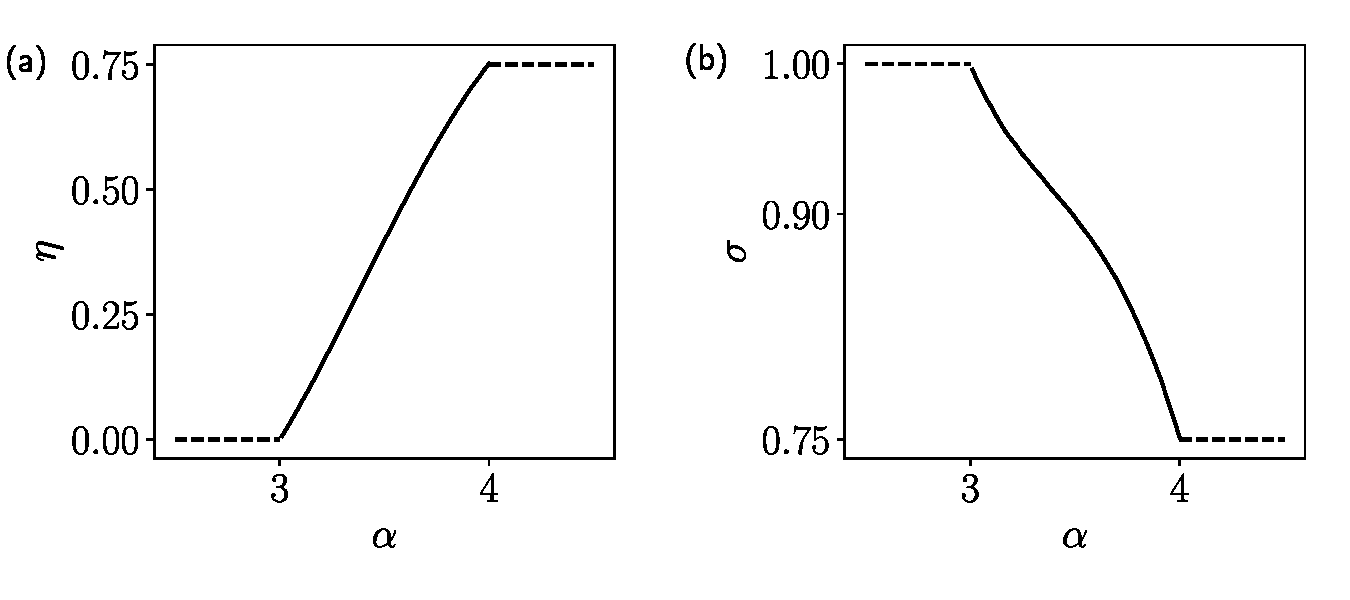
\includegraphics[width=0.9\textwidth]{Chapitre2/Figures/eta_kay.pdf}
	\caption{Evolution de l'exposant de rugosité (a) et de l'exposant d'hyperuniformité (b) associé avec la portée d'interaction dans le cadre théorique LR-CDP. Ces résultats encore non publiés ont été produits par K. Wiese qui nous a octroyé une autorisation de représentation dans ce manuscrit.}
	\label{fig:predic_kay}
\end{figure}

\subparagraph{}Un calcul similaire peut être mené pour déterminer l'exposant dynamique $z$ dans ce cadre. La transition de dépiégeage étant connue pour ne faire intervenir que deux exposants critiques indépendants, ces prédictions permettent en fait la caractérisation complète de la criticalité associée. En principe, les prédictions analytiques sont donc en mesure de déterminer complètement le cadre théorique LR-CDP. Toutefois, ces calculs restent soumis à des approximations et leur validation ne peut donc que venir de mesures numériques sur des modèles associés.

\section{Motivations pour une caractérisation numérique}

\subparagraph{}Dans cette section, nous motivons un peu plus spécifiquement la caractérisation numérique du cadre théorique LR-CDP en deux dimensions.

\subsection{Motivation principale : un point manquant dans la littérature}

\subparagraph{}De nombreuses études se sont déjà intéressées à l'influence d'un transport à longue portée sur le comportement critique des transitions de phase absorbantes. Dans le cadre de la percolation dirigée, cette influence a notamment été caractérisée de manière exhaustive en 1D \cite{hinrichsen_model_1999, hinrichsen_non_equilibrium_2007} et en 2D \cite{dos_santos_crossover_2018} sur des modèles de particules. Dans le cadre de la percolation dirigée conservée, cadre d'intérêt pour ce travail, les seules études numériques caractérisant l'impact de ce type d'interactions à longue portée viennent de l'étude de la transition de dépiégeage. Cependant, cette dernière trouvant essentiellement des réalisations physiques en 1D avec le cas de la ligne élastique, ces études se sont concentrés jusque là uniquement sur le cas unidimensionnel \cite{le_priol_long_range_2020, tanguy_individual_1998, rosso_roughness_2002, ramanathan_onset_1998}.

\subparagraph{}Dans ces travaux, les résultats numériques restent fidèles aux prédictions théoriques et confirment une évolution continue des exposants dans une gamme de portée déterminable par une analyse d'échelle. Toutefois, aucune étude à notre connaissance n'a été réalisée dans le cas d'un système appartenant à la classe CDP en 2D. Il manque alors à cette littérature un point de comparaison essentiel à notre étude dans les chapitres suivants. Par ailleurs cette caractérisation peut s'avérer utile en soi, simplement pour tester les prédictions analytiques présentées précédemment \cite{le_doussal_two_loop_2002}.

\subsection{Motivation secondaire : un cadre d'intérêt pour la modélisation de systèmes réels}

\subparagraph{}Bien que cela constitue notre motivation principale, la caractérisation de l'impact du transport à longue portée sur les systèmes de la classe CDP en 2D n'a pas seulement un intérêt théorique. En effet, certains modèles ou même certaines réalisations physiques correspondent vraisemblablement à cette situation. Cette étude peut alors permettre l'appréhension de leur criticalité plus spécifiquement.

\subparagraph{}Les réalisations physiques les plus évidentes de ce cadre sont celles associées à la transition de dépiégeage, de laquelle nous pouvons tirer deux exemples. Le premier est le mouvement de l'interface d'un fluide dans un milieu poreux par action de la gravité \cite{zhao_interface_2013}. Dans ce cas, le mouvement de l'interface bidimensionnelle peut être sujet à des interactions à longue portée permises par le fluide en volume. Le second concerne le mouvement des parois des domaines magnétiques dans les milieux magnétiques tridimensionnels \cite{alava_disorder_induced_1996}. Dans ce cas, ce sont les interactions entre charges magnétiques qui induisent la longue portée\cite{le_priol_long_range_2020}.

\subparagraph{}Un autre type de réalisations envisageables concerne les modèles épidémiques. Ces modèles que nous avons déjà introduit comme présentant une transition de phase absorbante ont de bonnes raisons de faire intervenir un transport à longue portée. En effet, dans ce cadre, celui-ci représente la capacité des vecteurs, i.e. des personnes, à se déplacer : par exemple une personne infectée prenant le train est susceptible de contaminer une autre personne à des centaines de kilomètres. La plupart des modèles épidémiologiques sont plutôt enclins à appartenir à la classe DP \cite{sanhedrai_epidemics_2022}. C'est notamment le cas du modèle SIS bien connu \cite{mota_critical_2018}. Toutefois, certains modèles plus complexes, faisant intervenir une diffusion locale des agents, peuvent présenter une criticalité différente, et dans une certaine limite, celle de la classe CDP \cite{nettuno_role_2024}. Dans ce cas, l'ajout d'un transport à longue portée pourrait donc effectivement être compris dans le cadre LR-CDP.

\subparagraph{}L'avantage du principe d'universalité est que, pour caractériser le comportement de tous ces systèmes, il suffit d'en caractériser un seul appartenant à la même classe. En étudiant un modèle numérique appartenant au cadre théorique LR-CDP en 2D, nous proposons une caractérisation de tous ces autres systèmes hypothétiques appartenant à la même classe. Ainsi, si l'intérêt principal de cette caractérisation numérique reste de constituer une base de comparaison pour l'étude des transitions de réversibilité et d'écoulement, elle trouve aussi un intérêt dans la modélisation de systèmes réels.

\section{Modèles}

\subparagraph{}Pour étudier l'influence du transport à longue portée dans la classe CDP en 2D, nous nous concentrons sur deux modèles emblématiques déjà présentés à la \autoref{sec:modelesCDP} : le modèle Manna et le ROM. Dans cette section, nous présentons l'implémentation numérique de ces deux modèles et leur généralisation par l'ajout d'un transport à longue portée. Cette généralisation nous permettra alors d'étudier le comportement critique de ces modèles numériques à n'importe quelle portée de transport pour ainsi confronter et compléter la théorie LR-CDP en 2D.

\subsection{LR-Manna}

\label{sec:ImplementationManna}

\subsubsection{Implémentation générale}

\subparagraph{}Nous commençons par présenter notre implémentation du modèle Manna. Le modèle Manna est un modèle très simple, appelant de ce fait une implémentation facilitée. Dans nos simulations, nous considérons un réseau 2D bipériodique de $N=L\times L$ sites, chacun indexé par un entier $i$, et positionné autour d'une position $\mathbf{r}_i = na\hat{\mathbf{e}}_x + ma \hat{\mathbf{e}}_y$ avec $(n,m) \in \mathbb{N}^2$. $a$ représente le pas du réseau. Sur l'ensemble de ces $N$ sites sont disposés initialement et de manière aléatoire $N_p$ particules.

\subparagraph{}\`A chaque pas de temps $t_i$ de la dynamique, les $n$ sites accueillant plus de $m$ particules sont considérés comme actifs. Ceux-ci redistribuent alors l'entièreté de leur masse (i.e. leurs particules) aux sites directement voisins, et ce de manière aléatoire. La redistribution de masse de tous les sites actifs se fait de manière synchrone, i.e. sur le même pas de temps. \`A la fin de cette redistribution, un nouveau pas de temps est initié.

\subparagraph{}L'activité du système au pas de temps $t_i$ est alors donnée par la proportion de sites actifs $A(t_i) = n(t_i)/N$. Par ailleurs, la densité de particules $\phi$ correspond simplement au rapport $\phi = N_p/N$ et peut donc prendre des valeurs plus ou moins grandes en fonction du seuil $m$ choisi. Ce modèle présente alors une transition de phase absorbante séparant une phase active où l'activité $A$ prend une valeur moyenne finie à temps long pour $\phi>\phi_c$, d'une phase absorbante où le système finit par tomber dans un état absorbant pour $\phi<\phi_c$. La valeur de la densité critique du système $\phi_c$ dépend des détails microscopiques d'implémentation choisis. Elle ne peut donc pas a priori être reprise de travaux précédents. 

\subsubsection{Transport à longue portée}

\subparagraph{}Dans le modèle Manna original, les particules sur les sites actifs font des sauts à courte portée. L’extension de cette dynamique au transport à longue portée y prend donc une forme évidente. Dans ce cas, les particules redistribuées ne le sont plus uniquement sur les sites voisins mais, à la place, celles-ci font des sauts $\mathbf{r}$ largement distribués selon :

\begin{equation}
	P(\mathbf{r}) \sim \frac{1}{r^\alpha}
\end{equation}

\noindent Dans un espace de dimension $D$, cela revient donc à effectuer des sauts de taille $\Delta = |\mathbf{r}|$, distribuée selon :

\begin{equation}
	P_\Delta(\Delta) \sim \frac{1}{\Delta^{1+\alpha-D}}
	\label{eq:sauts}
\end{equation}

\subparagraph{}Pour chaque particule sur un site actif, nous générons donc un nombre aléatoire $\Delta$ distribué de la sorte. Nous générons ensuite une direction aléatoire $\theta$ permettant de définir le déplacement $\Delta_x = \Delta \cos \theta$ selon $\hat{\mathbf{e}}_x$ et $\Delta_y = \Delta \sin \theta$ selon $\hat{\mathbf{e}}_y$. Les deux réels $\Delta_x$ et $\Delta_y$ sont alors convertis en entiers pour représenter une distance en nombre de sites. Enfin, les conditions aux limites périodiques sont appliquées pour déterminer le site d'arrivée de la particule. La procédure complète est résumée sur la \autoref{fig:LRModels}-(a).

\begin{figure}[h]
	\centering
	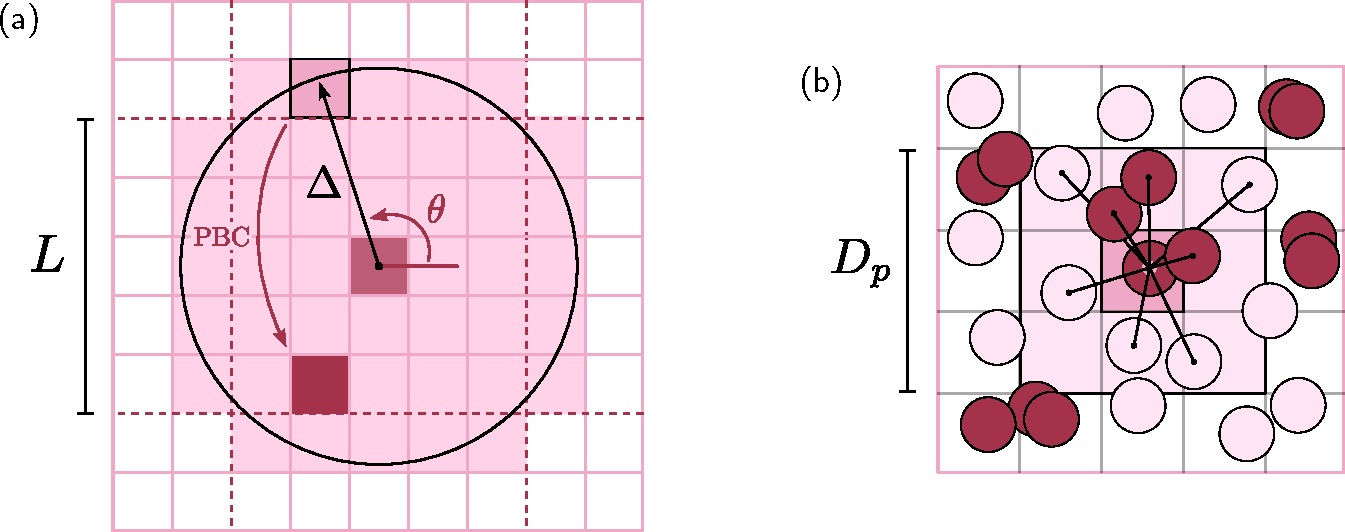
\includegraphics[width=\textwidth]{Chapitre2/Figures/Modeles/MannaJumps.pdf}
	\caption{Implémentation numérique des modèles LR-Manna et LR-ROM. (a) Procédure de saut à longue portée dans le modèle LR-Manna. PBC signifie \textit{periodic boundary conditions}. (b) Méthode cell-list pour la détermination des recouvrements dans le LR-ROM. En 2D, seules 9 cellules ont besoin d'être sondées pour déterminer les contacts d'une particules.}
	\label{fig:LRModels}
\end{figure}

\subparagraph{}Par cette implémentation numérique, il est possible d'étudier la transition de phase absorbante associée au modèle pour chaque portée $\alpha$. Dans la suite, nous appelons ce modèle généralisé LR-Manna.

\subsection{LR-ROM}

\label{sec:implementation_ROM}

\subsubsection{Implémentation générale}

\subparagraph{}Le second modèle que nous utilisons pour notre caractérisation numérique est le ROM. Ce modèle étant très proche du modèle Manna, son implémentation est très similaire. La différence principale qui les sépare vient du fait que la dynamique des particules a lieu dans ce cas en espace continu dans le ROM (par opposition au réseau de sites du modèle Manna). 

\subparagraph{}Pour son implémentation, $N_p$ particules de diamètre $D_p$ sont disposées initialement aléatoirement sur un espace 2D bipériodique de volume $L\times L$. Au début de chaque pas de temps $t_i$, les particules se recouvrant avec une autre particule sont considérées comme actives. Chaque particule active effectue alors un déplacement de manière synchrone décomposé en deux déplacements aléatoires $\Delta_x$ et $\Delta_y$, chacun de taille typique $a_p$. \`A l'issue de ce déplacement, un nouveau pas de temps est initié.

\subparagraph{}L'activité dans le ROM est définie comme la proportion de particules actives à un pas de temps donné et la densité $\phi$ comme la fraction d'espace occupée par les particules. Celles-ci étant choisies sphériques, nous avons $\phi = \frac{\pi D_p^2 N_p}{4 L^2}$ en 2D. De la même façon que le modèle Manna, le ROM ainsi défini présente une transition de phase absorbante de paramètre d'ordre $\phi$.

\subsubsection{Transport à longue portée}

\subparagraph{}Pour implémenter le transport à longue portée dans le ROM, nous utilisons exactement la même méthode que dans le cas du modèle Manna : à la place de faire des sauts finis de taille typique $a_p$, les particules actives font des sauts de taille $\Delta$ largement distribuée selon l'\autoref{eq:sauts}. Dans ce cas, nous nommerons cette généralisation du modèle LR-ROM.

\subsection{Détails d'implémentation}

\label{sec:DetImpl}

\subsubsection{Distributions de sauts}

\subparagraph{}Pour générer les sauts à longue portée dans les deux modèles, nous utilisons une méthode d'inversion \cite{devroye_general_1986} permettant générer des nombres aléatoires distribués selon :

\begin{equation}
	P_\Delta(\Delta) \sim \left\{
	\begin{aligned}
	& \Delta^{D-\alpha-1},\quad \text{si } \Delta > a\\
	& 0, \quad \text{sinon}
	\end{aligned}\right.
\end{equation}

\noindent le cut-off à petits $\Delta$ étant nécessaire à l'intégrabilité de la distribution pour $\alpha > D$. En pratique, nous commençons par tirer un nombre réel $x$ uniformément distribué dans $[0,1[$ grâce à des algorithmes pré-existants, puis $\Delta$ est obtenu par la transformation :

\begin{equation}
	\Delta = (1-x)^\frac{1}{D-\alpha}
\end{equation}

\subsubsection{Méthode cell-list dans le ROM}

\subparagraph{}Dans le ROM et le LR-ROM, la condition de recouvrement entre une particule située en $\mathbf{r}$ et une particule située en $\mathbf{r}^\prime$ correspond à $|\mathbf{r}-\mathbf{r}^\prime|<D_p$. Afin de déterminer si une particule est active au début d'un pas de temps, il est donc nécessaire de calculer sa distance à toutes les autres particules du système. En principe, ce calcul de distance admet une complexité d'ordre $N_p^2$, ce qui rend la recherche de recouvrement fastidieuse. Pour remédier à ce problème, nous utilisons une méthode dite cell-list \cite{allen_computer_2017} dont le principe est résumé à la \autoref{fig:LRModels}-(b).

\subparagraph{}Le principe de cette méthode est de découper l'espace de volume $L\times L$ en une collection de $ n \times n $ cellules de dimension $\frac{L}{n}\times \frac{L}{n}$. \`A chaque pas de temps, nous calculons à quelle cellule $i$ appartient chacune des $N_p$ particules. La portée de l'interaction de contact étant bornée par $D_p$, en choisissant $\frac{L}{n}=D_p$, seules les particules situées dans une cellule voisine\footnote{Ici la notion de voisinage prend en compte les conditions aux limites périodiques.} de la cellule $i$ sont susceptibles de recouvrir les particules situées dans la cellule $i$. Ainsi, cela restreint le calcul de distance à un sous-ensemble du système, diminuant alors la complexité de l'opération à l'ordre $N_p$.

\subsubsection{Parallélisation et implémentation GPU}

\subparagraph{}Les schémas numériques associés aux deux modèles sont relativement parallélisables. En effet, lors d'un pas de temps la mise à jour de la position des particules se fait de manière synchrone. De plus, lors de ce déplacement, aucun échange d'information n'est nécessaire entre les différents agents du système. Seules les conditions d'activité (recouvrement dans le ROM ou dépassement du seuil sur un site dans le modèle Manna), qui n'ont lieu qu'une fois par pas de temps, nécessitent un partage de la mémoire. 

\subparagraph{}Afin d'en tirer parti, nous implémentons donc ces deux modèles via le langage CUDA \cite{cuda} afin de réaliser les simulations sur GPU (cartes graphiques). Par opposition aux CPU, les GPU sont dotées d'un bien plus grand nombre de cœurs, permettant ainsi un plus grand nombre d'opérations simultanées. Ces cœurs sont individuellement moins performants mais les opérations nécessaires à la réalisation de la dynamique Manna sont très peu onéreuses et donc particulièrement adaptées à ce type d'architecture.

\subsubsection{Valeurs des paramètres}

\subparagraph{}Dans le ROM, nous prendrons comme unité de longueur du système le diamètre des particules et considèrerons donc $D_p=1$. Dans le cas de sauts à courte portée, nous prendrons $a_p=1$.

\subparagraph{}Dans le modèle Manna, nous prendrons comme unité de longueur du système le pas du réseau et donc $a=1$.

\section{Méthodes de caractérisation du comportement critique}

\label{sec:methodchap2}

\subparagraph{}La caractérisation du comportement critique d'un système ou d'une classe d'universalité passe par la détermination de ses exposants. Dans cette section, nous présentons les méthodes utilisées pour la détermination spécifique des exposants critiques $\beta$ et $\gamma^\prime$, de l'exposant dynamique $\delta$ et de l'exposant d'hyperuniformité $\sigma$, tous présentés au \autoref{chapter:introduction}. Ces méthodes nous permettront de caractériser les transitions dans le LR-ROM et le modèle LR-Manna pour chaque portée $\alpha$ et seront ensuite réutilisées dans les chapitres suivants. De ce fait, nous nous attachons à les décrire de manière suffisamment précise.

\subsection{Détermination des exposants critiques}

\label{sec:MethodesExposants}

\subsubsection{Détermination du point critique}

\subparagraph{}La première étape essentielle à la caractérisation d'une transition de phase est la localisation de son point critique. Ici, cela correspond à la détermination de la densité critique $\phi_c$. Pour la mettre en œuvre, nous nous appuyons sur la loi d'évolution du paramètre d'ordre dans le régime critique :

\begin{equation}
	\langle A \rangle \sim \delta\phi^\beta, \quad \delta\phi = \frac{\phi-\phi_c}{\phi_c}
\end{equation}

\noindent D'après celle-ci, la fonction $\langle A \rangle = f(\delta\phi)$ correspond à une droite de pente $\beta$ dans une représentation logarithmique. Cela peut donc représenter une méthode graphique pour la détermination de $\phi_c$ : la valeur recherchée est celle définissant la distance $\delta\phi$ permettant d'obtenir la courbe la plus proche d'une droite à petits $\delta\phi$. Si nous sous-estimons $\phi_c$, alors cette fonction montrera une courbure concave en échelle logarithmique. \`A l'inverse, si nous sur-estimons $\phi_c$, celle-ci montrera une courbure convexe. De cette manière, il est possible d'encadrer graphiquement la valeur adéquate de $\phi_c$ comme illustré à la \autoref{fig:PhicDeter}-(a). En pratique, afin de mieux percevoir les variations de forme de la courbe, nous examinons aussi l'évolution compensée $\langle A \rangle/\delta\phi^{\beta_t} = f(\delta\phi)$ par l'évolution attendue avec un exposant test $\beta_t$ en échelle log-lin (voir \autoref{fig:PhicDeter}-(b)). La méthode graphique d'encadrement associée est alors plus précise. Celle-ci permet donc de définir la densité critique $\phi_c$ et l'exposant $\beta$ comme les deux paramètres permettant d'obtenir une courbe constante à petits $\delta\phi$.

\begin{figure}[h]
	\centering
	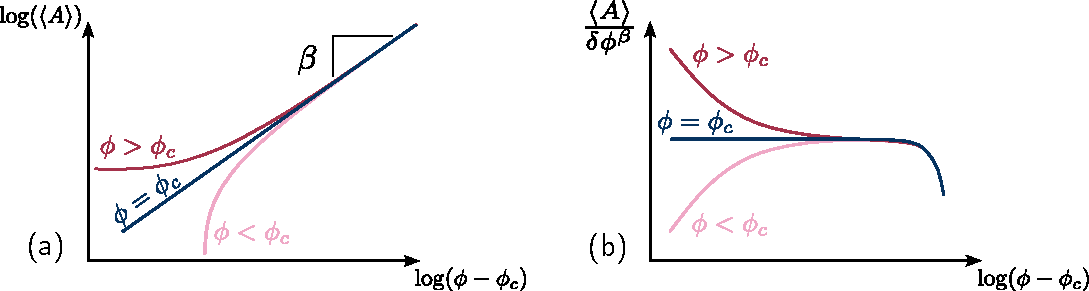
\includegraphics[width=\textwidth]{Chapitre2/Figures/Methodes/Phic.pdf}
	\caption{Méthode de détermination de la densité critique (a) en échelle logarithmique et (b) en échelle log-lin via une représentation compensée.}
	\label{fig:PhicDeter}
\end{figure}

\subparagraph{}Cette mesure repose donc finalement sur la détermination de la courbe $\langle A \rangle = f(\delta\phi)$ et donc sur les mesures précises de $\langle A \rangle$ pour différentes densités $\phi$. Pour réaliser ces mesures, à une taille $L$ de système donnée, nous laissons le système relaxer vers l'état stationnaire dans lequel nous mesurons la valeur moyenne de la variable instantanée $A(t)$. La détermination du régime stationnaire est effectuée graphiquement en représentant $A(t)$ en échelle logarithmique (voir \autoref{fig:DeltaDeter}). Afin de déterminer $\phi_c$, nous devons sonder le comportement du système proche du point critique et donc proche de la phase absorbante. Le problème est que, dans un système fini de taille $L$, les fluctuations de la dynamique peuvent amener le système dans un état absorbant même pour $\phi \gtrsim \phi_c$, rendant alors la détermination de $\langle A \rangle$ impossible. Les fluctuations critiques diminuant avec la taille du système $L$, il est possible de contourner cet obstacle en considérant des systèmes plus grands. La méthode que l'on choisit consiste alors à augmenter la taille $L$ du système à mesure que l'on considère des densités $\phi$ plus proches de $\phi_c$ afin de ne jamais risquer de tomber dans un état absorbant. In fine, la courbe $\langle A \rangle = f(\delta\phi)$ obtenue correspond donc  à une concaténation de courbes obtenues pour différentes tailles $L$ du système.

\subparagraph{}Ne pas se concentrer uniquement sur la plus grande taille $L$ envisageable est un choix permettant de réduire l'effort numérique associé. En effet, plus un système est grand, plus la simulation de sa dynamique est longue. Cette méthode suppose cependant que toutes ces courbes sont bien équivalentes, i.e. que $\phi_c$ est indépendant de $L$. En théorie, la valeur estimée de $phi_c$ sur un système de taille $L$ présente toujours une dépendance de taille finie, mais dans notre cas il est possible de s'en affranchir raisonnablement. En effet, statistiquement, si un système tombe dans l'état absorbant c'est parce que la longueur de corrélation $\xi$ de la dynamique associée est devenue au moins comparable à la taille $L$ de ce système. Or, par définition des effets de taille finie, la dépendance de $\phi_c$ en $L$ n'est visible que lorsque la dynamique "ressent" la taille du système, i.e. $\xi \gtrsim L$. Ainsi, en ne sondant que les états statistiquement non absorbés, nous pouvons considérer que $\phi_c$ est indépendante de $L$. Cette hypothèse se confirme alors très bien avec nos mesures puisque celles faites à différentes tailles de système se recouvrent parfaitement, comme représenté sur la \autoref{fig:Effet_Taille_Phic} dans le cas du modèle Manna. Toutefois, cela invite à ne pas sonder le système trop proche de sa limite d'absorption et de préférer systématiquement le passage à une taille supérieure.

\begin{figure}[h]
	\centering
	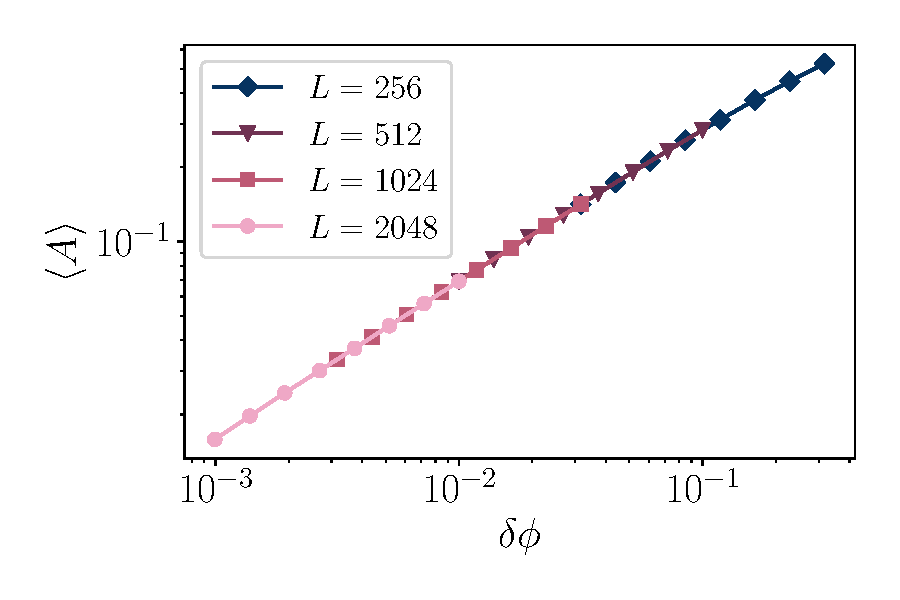
\includegraphics[width=0.6\textwidth]{Chapitre2/Figures/Phi_cindep.pdf}
	\caption{Détermination de la courbe $\langle A \rangle = f(\delta\phi)$ dans le ROM. La superposition des courbes pour différentes tailles de système dans leur domaine de non-absorption valide l'approche considérant $\phi_c$ indépendante de $L$. Ici, on a $\phi_c \approx 0.23520$}
	\label{fig:Effet_Taille_Phic}
\end{figure}

\subsubsection{Détermination des exposants statiques}

\subparagraph{}Une fois la densité critique $\phi_c$ déterminée précisément pour un système, il est possible de mesurer les exposants critiques de la transition. L'exposant statique $\beta$ est en fait déjà déterminé lors de la détermination de $\phi_c$ via les méthodes graphiques présentées précédemment. Afin d'obtenir un ordre de grandeur de son incertitude, nous effectuons un ajustement de la courbe $\langle A \rangle = f(\delta\phi)$ à petits $\delta\phi$ en échelle logarithmique pour les deux valeurs extrémales de l'encadrement de $\phi_c$.

\subparagraph{}Pour déterminer l'exposant des fluctuations critiques $\gamma^\prime$, nous mesurons la variance de l'activité $\langle \delta A^2\rangle$ dans l'état stationnaire sur les mêmes courbes $A(t)$ qui ont permis de mesurer $\langle A \rangle$. La densité critique ayant été précédemment déterminée, nous déterminons $\gamma^\prime$ directement par ajustement de la courbe $\langle \delta A^2\rangle = g(\delta\phi)$ en échelle logarithmique. La variance correspondant à un moment d'ordre supérieur par rapport à la moyenne, sa détermination précise est plus délicate. Ainsi, la détermination de $\gamma^\prime$ sera généralement entachée de plus grandes erreurs. Toutefois, étant donné que nous nous concentrerons essentiellement sur l'évolution de $\gamma^\prime$ avec la portée dans la suite de ce travail, nous nous satisferons d'une telle précision. Les incertitudes sur cette détermination sont associées à l'incertitude sur l'ajustement de la courbe en échelle logarithmique\footnote{En pratique, nous constatons que les incertitudes sur $\gamma^\prime$ liées à la détermination de $\phi_c$ (et donc la définition de $\delta\phi$) sont négligeables devant l'incertitude de l'ajustement effectué à une valeur de $\phi_c$ donnée.}.

\subsubsection{Détermination de l'exposant dynamique}

\subparagraph{}Comme nous l'avons vu au \autoref{chapter:introduction}, en partant d'une configuration initiale aléatoire, proche du point critique, le système relaxe vers l'état stationnaire de manière algébrique :

\begin{equation}
	A(t) \sim t^{-\delta}
	\label{eq:deltaJumps}
\end{equation}

\noindent L'exposant $\delta$ ainsi défini permet de caractériser la transition d'un point de vue dynamique. Une difficulté liée à sa détermination est que le régime de temps dans lequel le comportement de l'\autoref{eq:deltaJumps} est valable est situé entre un comportement non-universel à temps courts et une saturation à temps long du fait que $\phi>\phi_c$. Il n'est donc pas aisé de mesurer $\delta$ par un simple ajustement sur une unique courbe. 

\subparagraph{}Pour remédier à ce problème, nous utilisons une méthode de redimensionnement comme outil de détermination plus précis. Pour ce faire, nous nous appuyons sur le fait que, hors du régime de temps courts, l'activité dans le système prend la forme :

\begin{equation}
	A(t, \delta\phi) \sim \langle A \rangle (\delta\phi) + t^{-\delta} \sim \delta\phi^\beta + t^{-\delta} \Rightarrow \frac{A(t)}{\delta\phi^\beta} \sim 1 + \left(\frac{t}{\delta\phi^{\beta/\delta}}\right)^{-\delta}
\end{equation}

\noindent par définition de l'exposant $\beta$. Ainsi, si nous redimensionnons $A(t)$ par $\delta\phi^\beta$ et $t$ par $\delta\phi^{\beta/\delta}$, nous obtenons une évolution indépendante de la distance au point critique $\delta\phi$. En d'autres termes, si l'on mesure l'évolution $\frac{A(t)}{\delta\phi^\beta} = f \left(\frac{t}{\delta\phi^{\beta/\delta}} \right)$ pour différentes densités $\phi$, les différentes évolutions se superposent graphiquement (voir \autoref{fig:DeltaDeter}). $\beta$ et $\phi_c$ étant précédemment mesurés, $\delta$ est alors déterminé comme l'exposant qui permet la superposition de toutes les courbes sur une courbe maîtresse sous ce redimensionnement. L'incertitude de mesure sur cet exposant est alors donnée par la gamme d'exposants pour laquelle la superposition des courbes est jugée satisfaisante. Ce principe de mesure par redimensionnement s'avère très efficace, et sera utilisé à plusieurs reprises dans les chapitres suivants pour mesurer d'autres quantités.

\begin{figure}[h]
	\centering
	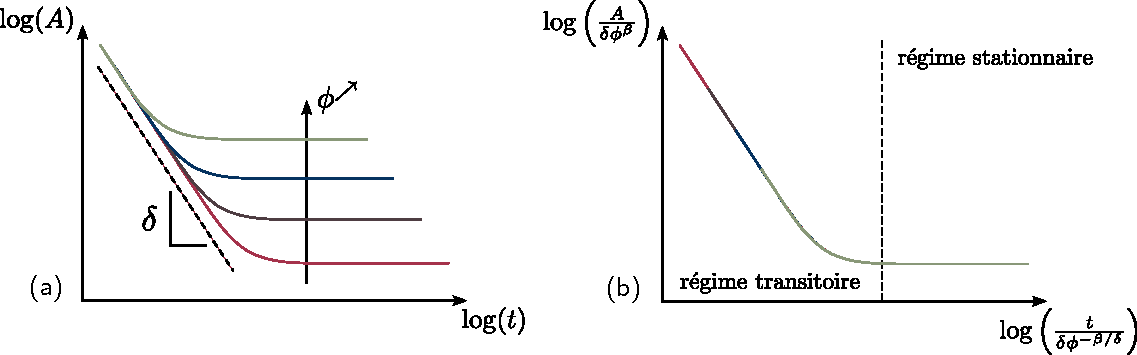
\includegraphics[width=\textwidth]{Chapitre2/Figures/Methodes/Delta.pdf}
	\caption{Méthode de détermination de l'exposant dynamique $\delta$. (a) Évolution de l'activité dans le système en fonction du temps pour différentes densités $\phi$. (b) Redimensionnement du temps et de l'activité par la distance au point critique permettant la superposition des différentes courbes sur une courbe maîtresse.}
	\label{fig:DeltaDeter}
\end{figure}

\subsection{Caractérisation de l'hyperuniformité}

\label{sec:MethodHU}

\subparagraph{}Dans cette dernière sous-section nous présentons les méthodes utilisées pour sonder les propriétés d'hyperuniformité dans nos modèles. Celles-ci reposant sur des propriétés de structure, nous ne pouvons pas nous limiter à une étude du comportement macroscopique pour déterminer l'exposant $\sigma$. Toutefois, la philosophie des mesures utilisées en pratique restent très similaires.

\subsubsection{Mesure directe du facteur de structure}

\subparagraph{}Comme nous l'avons évoqué au \autoref{chapter:introduction}, les systèmes appartenant à la classe CDP présentent des propriétés hyperuniformes. Proche de la transition, la répartition des particules dans l'espace présente des corrélations à longue portée. Une manière de les caractériser  est de passer dans l'espace réciproque. En effet, dans de tels systèmes, cette propriété se traduit par une diminution du facteur de structure $S(\mathbf{q})$ à petits $q$ selon :

\begin{equation}
	S(\mathbf{q})\sim q^{\alpha_\text{HU}}, \quad 0 < \alpha_\text{HU} < 1
\end{equation}

\noindent L'exposant $\alpha_\text{HU}$ permet alors de caractériser la transition de phase au même titre qu'un autre exposant critique. Le cas limite $\alpha_\text{HU}$ = 0 représente une répartition totalement décorrélée à grande échelle.

\subparagraph{}Une manière de quantifier l'hyperuniformité caractéristique d'un comportement critique est donc de mesurer précisément le facteur de structure à petits $q$ dans un état stationnaire proche du point critique afin d'en déduire une estimation de cet exposant $\alpha_\text{HU}$.

\subsubsection{Méthode de box-counting}

\paragraph{Définition}

\subparagraph{}Une autre façon de procéder est de revenir à la définition initiale de l'hyperuniformité \cite{torquato_local_2003}. Comme nous l'avons présenté à la \autoref{sec:introHU}, dans un système hyperuniforme, la variance $\langle \delta n^2\rangle_l$ du nombre de particules contenues dans un sous-ensemble du système de volume $l^D$ se comporte comme :

\begin{equation}
	\langle \delta n^2\rangle_l \sim \langle n \rangle_l^\sigma , \quad  \sigma < 1
	\label{eq:HUBC}
\end{equation}

\noindent $\sigma = 1$ représentant le cas trivial de l'absence de corrélations. Cette représentation de l'hyperuniformité est en fait directement liée à celle observée dans l'espace réciproque, les exposants $\sigma$ et $\alpha_\text{HU}$ étant reliés par la relation \cite{torquato_local_2003, lei_non_equilibrium_2024, hexner_hyperuniformity_2015} :

\begin{equation}
	\sigma = \left\{
	\begin{aligned}
	&1-\frac{\alpha_\text{HU}}{D}, \quad\text{si } 0 < \alpha_\text{HU} < 1 \\
	&1-\frac{1}{D}, \quad \text{si } \alpha_\text{HU} > 1
	\end{aligned}
	\right.
	\label{eq:eqsigmaalphahu}
\end{equation}

\subparagraph{}Une méthode de qualification de l'hyperuniformité, que nous appelons méthode box-counting, consiste donc à mesurer $\langle \delta n^2\rangle_l$ et pour différentes tailles $l$ de sous-ensembles dans des configurations de l'état stationnaire du système proche de son point critique. Ainsi, nous pouvons étudier son évolution en fonction de $\langle n \rangle_l$ pour déterminer directement l'exposant $\sigma$ associé.

\subparagraph{}Si la définition de l'hyperuniformité s'est construite autour de l'\autoref{eq:HUBC}, plusieurs travaux s'intéressent aux fluctuations de densité locale $\langle \delta \rho^2\rangle_l$ au lieu du nombre de particules, et en fonction de l'extension $l$ du sous-ensemble au lieu du nombre moyen de particules \cite{hexner_hyperuniformity_2015, bub_lee_hyperuniformity_2019}. Dans ce cas, on définit la loi d'échelle entre ces quantités par l'exposant $\lambda$ selon :

\begin{equation}
	\langle \delta \rho^2\rangle_l \sim l^{-\lambda}
\end{equation}

\noindent qui est alors directement relié à l'exposant $\sigma$ par :

\begin{equation}
	\sigma = 2 - \frac{\lambda}{D}
\end{equation}

\paragraph{Implémentation}

\subparagraph{}Dans ce chapitre, nous caractérisons l'hyperuniformité des modèles de sauts à longue portée via la méthode de box-counting. Pour ce faire, nous générons des configurations par la dynamique stationnaire de systèmes proches du point critique. Chacune de ces configurations est alors analysée de la même façon.

\subparagraph{}Pour le modèle Manna comme pour le ROM, nous découpons l'espace carré de surface $L\times L$ en une collection compacte de sous-ensembles carrés de taille $l\times l$. En comptant le nombre de particules présentes dans chacun de ces sous-ensembles, nous en déduisons la variance $\langle \delta n^2\rangle_l$ associée. Le nombre moyen de particules dans les sous-ensembles est directement donné par  $\langle n \rangle_l= \phi \times l^D$. Si à petits $\langle n \rangle_l$ l'évolution est satisfaisante avec une mesure unique, celle à grande échelle nécessite un certain effort numérique. La première raison évidente est le manque d'échantillonnage aux grandes échelles dans les configurations de taille finie : plus $l$ est grand, moins il y a de sous-compartiments. La seconde raison est que les fluctuations à grande échelle sont associées à des temps de corrélation plus grands, ce qui implique une forte séparation temporelle entre deux configurations quasi-indépendantes dans l'état stationnaire. Afin d'obtenir une statistique raisonnable, chaque mesure associée à une densité $\phi$ et une portée $\alpha$ est donc moyennée dans le temps et sur différents états initiaux complètement décorrélés les uns des autres.

\paragraph{Détermination par redimensionnement}

\subparagraph{}En principe, la forme définie par l'\autoref{eq:HUBC} n'est valable qu'à des échelles de longueur $l$ suffisamment grandes, soit $\langle n \rangle_l \gg 1$. Pour mesurer l'exposant $\sigma$, il est donc nécessaire se placer à grande échelle. Par ailleurs, pour sonder un état stationnaire, il est aussi nécessaire se placer à une distance finie $\delta\phi>0$ du point critique, sans quoi le système tombera dans un état absorbant. Cette distance finie du point critique définit alors une échelle de longueur $l_c$, ou de manière équivalente un cut-off $\langle n \rangle_c$, au-delà de laquelle l'évolution algébrique n'est plus valide. En fait, dans nos mesures, au-delà de cette échelle de longueur, la courbe $\langle \delta n^2 \rangle = f(\langle n \rangle)$ présente un crossover non monotone vers l'évolution triviale $\sigma = 1$, aussi distinguable sur l'évolution du facteur de structure \cite{hexner_hyperuniformity_2015,hexner_noise_2017, hexner_enhanced_2017 }. En pratique, au-delà de $l_c$, avant que l'exposant effectif local de la courbe $\langle \delta n^2 \rangle = f(\langle n \rangle)$ ne rejoigne le cas décorrélé avec $\sigma_\text{eff}=1$, il diminue ($\sigma_\text{eff}<\sigma$). Cette diminution est visible sur les évolutions représentées à la \autoref{fig:HUCM} par exemple. L'évolution globale de $\langle \delta n^2 \rangle$ à grands $\langle n \rangle$ peut donc être modélisée par l'équation suivante :

\begin{equation}
	\langle \delta n^2 \rangle \sim \langle n \rangle^\sigma g\left( \frac{\langle n \rangle}{\langle n \rangle_c} \right)
\end{equation}

\noindent avec $g$ une fonction initialement décroissante définissant la forme du crossover.

\subparagraph{}Du fait de la présence de deux crossovers, un de petite taille et un dû à la distance finie au point critique, il peut s'avérer difficile de mesurer l'exposant $\sigma$ ou $\lambda$ sur une unique courbe. Une méthode utilisée dans \cite{hexner_hyperuniformity_2015} consiste alors à étudier différentes courbes associées à différentes distances du point critique $\delta\phi$. En supposant que l'échelle de longueur définissant le cut-off se comporte comme la longueur de corrélation $\xi\sim \delta\phi^{-\nu_\perp}$, nous avons $\langle n \rangle_c \sim \delta\phi^{-D\nu_\perp}$. Ainsi, en redimensionnant $\langle n \rangle$ par $ \delta\phi^{-D\nu_\perp}$ et $\langle \delta n^2 \rangle$ par $\delta\phi^{-\nu_\perp D \sigma}$, les courbes obtenues pour différentes densités devraient se superposer sur une même courbe maîtresse. Cela définit alors une potentielle méthode graphique pour la mesure de $\sigma$, utilisant les effets de crossover à son avantage. Néanmoins, en pratique, cette méthode peut s'avérer coûteuse numériquement car elle suppose la détermination précise d'un ensemble de courbes à différentes densités $\phi$. C'est pourquoi, nous ne l'utiliserons que dans le cas d'une analyse plus poussée.

\subsubsection{Des mesures complexes}

\subparagraph{}Si l'hyperuniformité n'a jamais été mesurée dans les modèles de transport à longue portée, celle-ci a fait l'objet de nombreuses études dans le cas de courte portée. Notamment, le ROM et le modèle Manna ont été caractérisés en ce sens à plusieurs reprises.

\subparagraph{}Les première études ont été menées par Hexner et Levine \cite{hexner_hyperuniformity_2015}, Tjhung et Berthier \cite{tjhung_hyperuniform_2015} et Weijs et al \cite{weijs_emergent_2015}. Dans \cite{tjhung_hyperuniform_2015}, les auteurs ont mesuré proche de la transition un exposant $\alpha_\text{HU} \approx 0.45$ dans le cas du ROM en 2D. En parallèle, l'étude \cite{hexner_hyperuniformity_2015} s'est concentrée sur les propriétés de différents modèles appartenant à la classe CDP, dont le modèle Manna et le ROM. Dans le cas bidimensionnel, il a été déterminé $\lambda\approx 2.45$ et $\alpha_\text{HU}\approx 0.45$, deux mesures cohérentes et indiquant $\sigma \approx 0.775$. Ces valeurs ont alors été confirmées dans \cite{weijs_emergent_2015} et comparées à une situation expérimentale. Par la suite, ces résultats furent retrouvés dans des généralisations de ces modèles \cite{hexner_noise_2017, ma_hyperuniformity_2019}.

\subparagraph{}Les résultats précédents confortent l'idée que les exposants d'hyperuniformité sont universels, i.e. communs à tous les modèles de la classe CDP. Toutefois, une étude plus récente semble mettre en défaut cette idée. Dans \cite{bub_lee_hyperuniformity_2019}, en utilisant des tailles de systèmes plus grandes que dans les études précédentes, les auteurs semblent relever une légère différence de l'ordre de 5\% entre les exposants d'hyperuniformité du ROM et du modèle Manna en 2D, qualifiant alors l'hyperuniformité de "faiblement universelle" dans ces modèles. Dans \cite{wiese_hyperuniformity_2024}, il a par ailleurs été montré que les mesures d'hyperuniformité peuvent être soumises à de forts effets de taille finie, affectant significativement les résultats des mesures. Sans nécessairement remettre en question l'universalité des propriétés hyperuniformes, ces études nous invitent donc à questionner nos méthodes et rester critique face aux mesures que nous présenterons.

\section{Exposants critiques}

\subparagraph{}Afin de préciser quantitativement l'évolution des exposants critiques dans le cadre LR-CDP en 2D, nous nous concentrons d'abord sur sa représentation par le modèle LR-ROM. Dans cette section, nous présentons les résultats obtenus quant à la caractérisation des exposants critiques associés à chaque portée de transport $\alpha$.

\subparagraph{}Dans la \autoref{sec:LRCanonique} nous avons vu que dans ce cadre nous attendions une évolution continue de la criticalité entre $\alpha = 4$ et $\alpha=3$. Pour $\alpha\geq 4$ nous nous attendons à retrouver les valeurs des exposants reportées à la première ligne du \autoref{tab:expocrit_LRROM}. Pour $\alpha\leq 3$, nous nous attendons à retrouver les valeurs triviales des exposants associés au champ moyen. Pour cerner et caractériser précisément la zone d'évolution continue des exposants, nous nous attachons par la suite à caractériser les portées de transport dictées par $\alpha \in \{ 6, 5, 4, 3.75, 3.5, 3.25, 3, 2.5  \}$.

\label{sec:expcritjumps}

\subsection{Exposants statiques}

\subparagraph{}En appliquant les méthodes décrites à la \autoref{sec:MethodesExposants}, nous déterminons les densités critiques $\phi_c$ des systèmes pour chacune des portées $\alpha$. Pour ce faire, nous utilisons des tailles de systèmes allant jusqu'à $L=16384$, correspondant à des nombres de particules allant jusqu'à $N\approx 6\times 10^7$. Un exemple de détermination est représentée à la \autoref{fig:DeterPhicJumps} dans le cas $\alpha = 3.75$. Les exposants $\beta$ et $\gamma^\prime$ et leurs incertitudes sont alors mesurés, leurs valeurs sont reportées dans le \autoref{tab:expocrit_LRROM} et leurs évolutions sont représentées à la \autoref{fig:EvolExpJumps}.

\begin{figure}[h]
	\centering
	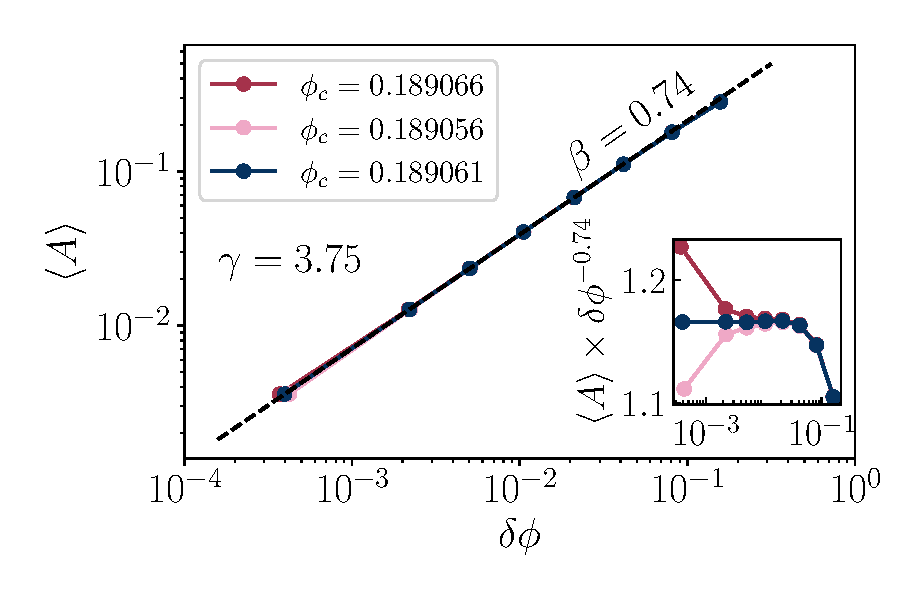
\includegraphics[width=0.7\textwidth]{Chapitre2/Figures/Exposants/Deter_phic_gamma375_LRROM.pdf}
	\caption{Détermination de la densité critique dans le LR-ROM pour $\alpha=3.75$. En encart, la représentation compensée permet de distinguer clairement $\phi_c = 0.189061$ comme une meilleure estimation que $\phi_c = 0.189056$ et $\phi_c = 0.189066$}
	\label{fig:DeterPhicJumps}
\end{figure}

\subparagraph{}Dans la limite de courte portée, nous retrouvons le comportement critique associé à la classe CDP. Pour $\alpha > 4$, nous mesurons $\beta\approx 0.63$ et $\gamma^\prime \approx 0.37$, tous deux en accord avec $\beta_\text{CDP}^{2D}\approx 0.64$ et $\gamma_\text{CDP}^{\prime 2D}\approx 0.37$. \`A l'opposé, dans la limite de longue portée, nous retrouvons les exposants associés au champ moyen de la classe CDP. Notamment, pour $\alpha = 2.5$, l'accord est exact dans la limite des incertitudes de détermination. L'évolution des exposants prend majoritairement place entre $\alpha = 4$ et $\alpha = 3$, en accord avec le cadre théorique. Toutefois, nous notons un léger écart avec les valeurs attendues au niveau de ces bornes. Notamment, pour $\alpha = 4$, nous mesurons $\beta \approx 0.69$ soit une valeur légèrement supérieure à celle associée à la courte portée. Nous discuterons de l'origine potentielle de cet écart dans la section suivante.

\subparagraph{}En pratique, la détermination de l'exposant $\nu_\perp$ nécessite l'analyse des corrélations spatiales d'activité dans le système afin d'en déduire la longueur de corrélation $\xi$ associée. Toutefois, il existe une relation d'échelle entre les exposants $\beta$, $\gamma^\prime$ et $\nu_\perp$, présentée au \autoref{chapter:introduction} :

\begin{equation}
	2\beta + \gamma^\prime = \nu_\perp D
	\label{eq:HyperScaling}
\end{equation}

\noindent En supposant que celle-ci reste valable à n'importe quelle portée en-dessous de la dimension critique $D_c = 2(\alpha-D)$, nous pouvons tirer profit de cette relation pour dériver l'exposant $\nu_\perp$ associé. En utilisant les valeurs mesurées de $\beta$ et $\gamma^\prime$, nous répertorions dans le \autoref{tab:expocrit_LRROM} la valeur $\nu_\perp^*$ déduite de cette relation. Comme nous l'avons mentionné à la \autoref{sec:LRCanonique}, la subtilité est que, en présence d'interactions à longue portée, la valeur champ moyen de cet exposant est donnée par $\nu_\perp = 1/(\alpha-D)$, et donc dépendante de $\alpha$. En gardant cela en mémoire, nous observons de la même façon que les valeurs de $\nu_\perp^*$ suivent une évolution continue de la limite de courte portée avec $\nu_\perp \approx 0.82$ pour $\alpha>4$ à la limite de champ moyen avec $\nu_\perp\approx 1 = 1/(\alpha-D)$ pour $\alpha=3$. Pour $\alpha < 3$, nous avons $D>D_c$ et il n'est donc plus possible d'utiliser la relation d'échelle pour déterminer $\nu_\perp$. 

%\begin{figure}[h]
%	\centering
%	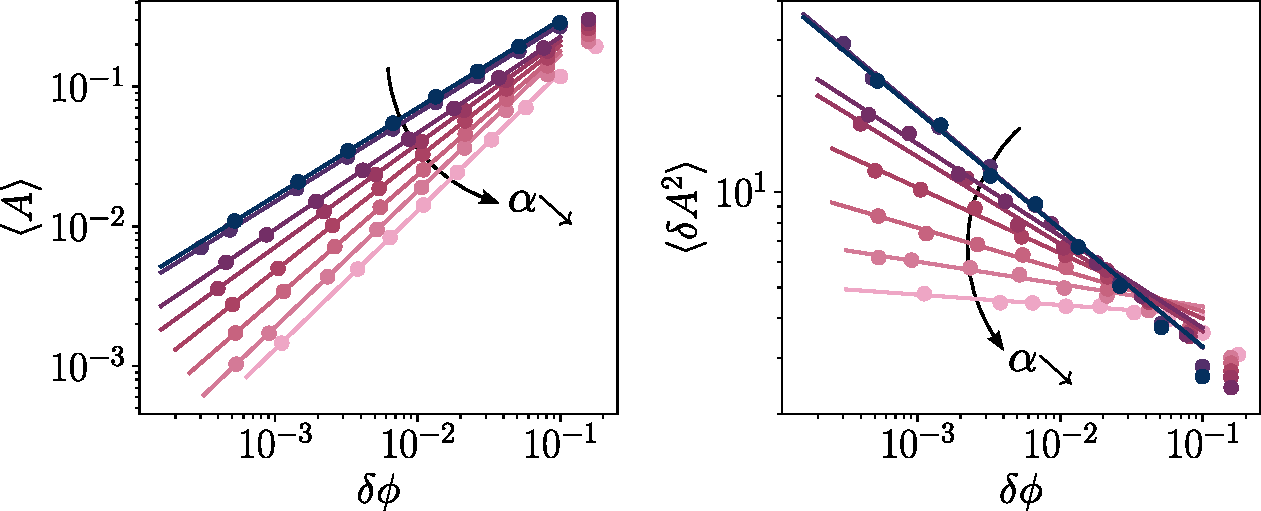
\includegraphics[width=\textwidth]{Chapitre2/Figures/Exposants/EvolMeanVar_Jumps.pdf}
%	\caption{}
%	\label{fig:EvolMeanVarJumps}
%\end{figure}

\subsection{Exposant dynamique}

\label{sec:expdynjump}

\subparagraph{}L'exposant dynamique $\delta$ est ensuite déterminé pour chaque portée $\alpha$ en suivant la méthode de redimensionnement précédemment présentée. Un exemple de détermination est présenté pour $\alpha = 4$ à la \autoref{fig:DeltaDeterJumps}. Les valeurs estimées sont reportées dans le \autoref{tab:expocrit_LRROM} et leur évolution est représentée à la \autoref{fig:EvolExpJumps}.

\begin{figure}[h]
	\centering
	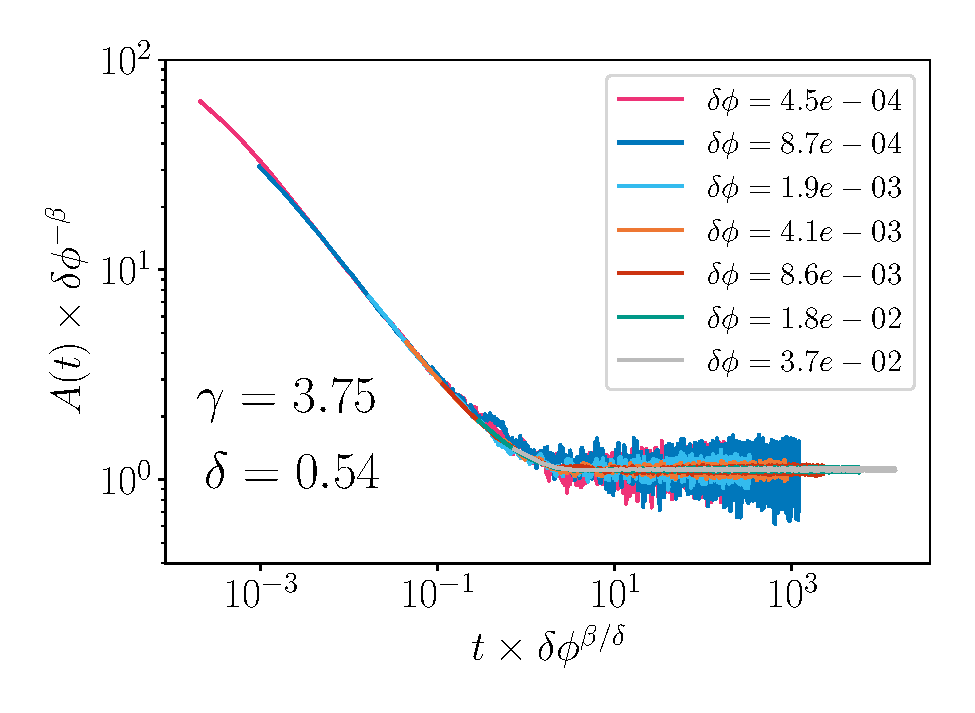
\includegraphics[width=0.7\textwidth]{Chapitre2/Figures/Exposants/DeltaDeter.pdf}
	\caption{Détermination de l'exposant dynamique $\delta$ par redimensionnement dans le LR-ROM pour $\alpha=3.75$.}
	\label{fig:DeltaDeterJumps}
\end{figure}

\subparagraph{}Comme dans le cas des exposants statiques, nous retrouvons les comportements limites de champ moyen $\delta_\text{CDP}^\text{CM}=1$ et de courte portée $\delta_\text{CDP}^{2D} \approx 0.42$ dans la limite des petits et des grands $\alpha$. De la même façon, l'évolution significative de l'exposant a lieu dans la gamme $3<\alpha<4$ bien que nous notions encore une fois un léger écart aux valeurs attendues au niveau de ces bornes.

\begin{figure}[h]
	\centering	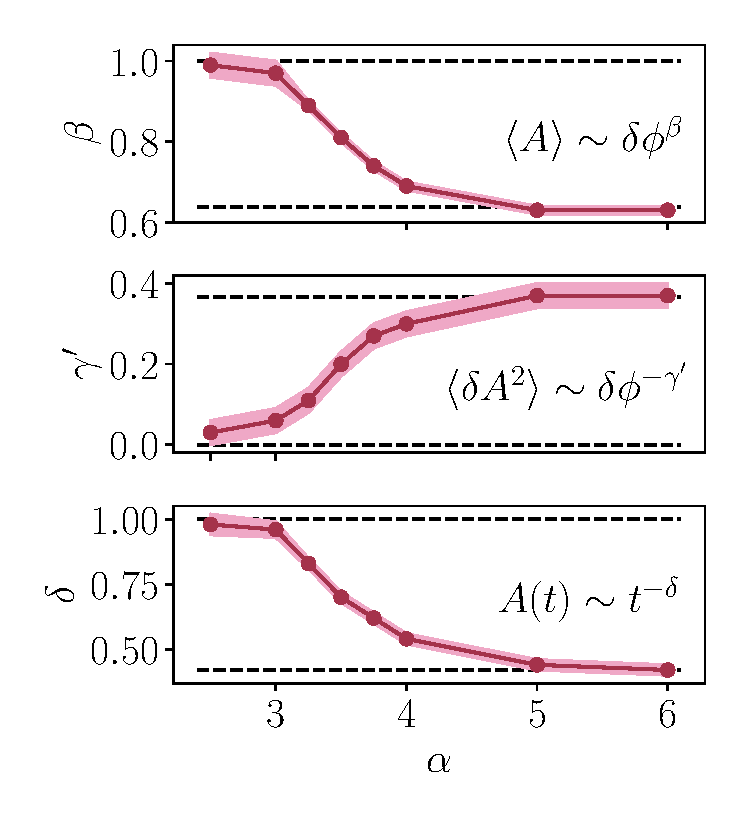
\includegraphics[width=0.6\textwidth]{Chapitre2/Figures/Exposants/exp_suspensions_jumps.pdf}
	\caption{Évolution des exposants critiques $\beta$, $\gamma^\prime$ et $\delta$  avec la portée dans les modèles LR-ROM. Les zones colorées en rose représentent les incertitudes de détermination.}
	\label{fig:EvolExpJumps}
\end{figure}

\subparagraph{}Finalement, l'estimation des exposants critiques dans le modèle LR-ROM confirme l'inscription des interactions de transport à longue portée dans le cadre théorique LR-CDP présenté à la \autoref{sec:LRCanonique}. En augmentant la portée du transport de matière dans le système, la criticalité passe continûment de son équivalent de courte portée à son équivalent de champ moyen, gardant une évolution concave du paramètre d'ordre ($\beta < 1$) et une divergence des fluctuations à l'approche du point critique ($\gamma^\prime>0$). Au premier ordre, cette évolution prend effectivement place dans la zone $3D/2 < \alpha < D+2$ soit $3<\alpha<4$ dans le cas bidimensionnel.

\begin{table}[h]
\centering
\begin{tabular}{cccccc}
\hline \hline $\alpha$ & $\beta$ & $\gamma^\prime$ & $\delta$ & $\nu_\perp^*$ & $\nu_\perp^\text{CM}$\\
\hline \text{CDP} \cite{lubeck_universal_2004} & 0.64 & 0.37 & 0.42 & 0.80 & 0.50\\
6 & 0.63 & 0.37 & 0.42 & 0.82 & 0.50\\
5 & 0.63 & 0.37 & 0.44 & 0.82 & 0.50\\
4 & 0.69 & 0.30 & 0.54 & 0.84 & 0.50\\
3.75 & 0.74 & 0.27 & 0.62 & 0.88 & 0.57\\
3.5 & 0.81 & 0.20 & 0.70 & 0.91 & 0.67\\
3.25 & 0.89 & 0.11 & 0.83 & 0.95 & 0.80\\
3 & 0.98 & 0.06 & 0.96 & 1.01 & 1.00\\
2.5 & 0.99 & 0.03 & 0.98 & - & 2.00\\
\hline \hline
\end{tabular}
\caption{Exposants critiques $\beta$, $\gamma^\prime$ et $\delta$ déterminés dans les modèles LR-ROM en 2D. La troisième colonne représente l'exposant $\nu_\perp$ dérivé par la relation d'échelle (\autoref{eq:HyperScaling}) et la quatrième l'exposant champ moyen associé à chaque portée $\alpha$}
\label{tab:expocrit_LRROM}
\end{table}

\section{Hyperuniformité}

\subparagraph{}Dans cette dernière section, nous proposons de conclure la caractérisation quantitative du cadre théorique LR-CDP en 2D en nous intéressant à l'évolution de l'hyperuniformité. Dans la \autoref{sec:LRCanonique}, nous avons vu que dans ce cadre nous attendions une évolution continue de l'exposant d'hyperuniformité $\sigma$ entre $\alpha = 4$ et $\alpha=3$. Dans la limite de courte portée $\alpha \geq 4$, la théorie développée par mapping avec le dépiégeage \cite{wiese_hyperuniformity_2024} prédit $\sigma = 0.75$ tandis qu'elle prédit $\sigma = 1$ à $\alpha = 3$. Entre ces deux limites, des calculs issus du groupe de renormalisation fonctionnel permettent de prédire l'évolution de l'exposant $\sigma$ avec $\alpha$. Dans la suite de cette étude, nous proposons de confronter ces calculs théoriques via la caractérisation des propriétés hyperuniformes des modèles LR-ROM et LR-Manna pour différentes portées de transport $\alpha$. Ce travail, mené en collaboration étroite avec K. Wiese, est encore au stade préliminaire mais les premiers résultats associés soulèvent des points intéressants qu'il semble judicieux de faire figurer dans cette thèse, bien qu'ils n'en constituent pas l'objet principal. Notamment, nous montrons que les mesures d'hyperuniformité dans ces modèles se révèlent particulièrement exigeantes.

\label{sec:HUjumps}

\subsection{Hyperuniformité dans le LR-ROM}

\subparagraph{}En utilisant la méthode de box-counting présentée à la \autoref{sec:MethodHU}, nous commençons par caractériser les propriétés hyperuniformes des transitions du LR-ROM pour $\alpha\in\{ 5, 4, 3.75, 3.5, 3.25, 3 \}$. Afin d'opérer une comparaison juste entre toutes ces portées, nous étudions chacune d'elle pour une distance similaire au point critique $\delta\phi \approx 1\times 10^{-3}$ et une taille de système $L=4096$.

\begin{figure}[h]
	\centering	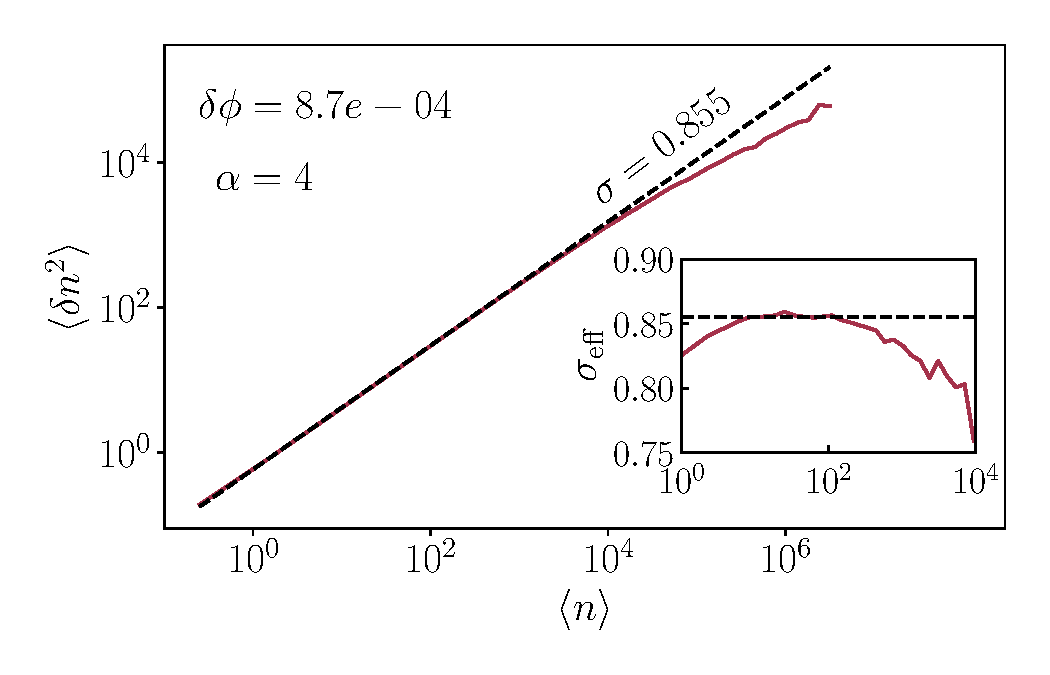
\includegraphics[width=0.65\textwidth]{Chapitre2/Figures/Hyperuniformity/FigHULRROM.pdf}
	\caption{Estimation de l'exposant d'hyperuniformité $\sigma$ dans le LR-ROM pour $\alpha=4$. En encart, l'exposant effectif local, déterminé comme la dérivée logarithmique de la courbe représentée en figure principale.}
	\label{fig:ExHUJumps}
\end{figure}

\subparagraph{}Nous présentons un exemple de mesure obtenue pour $\alpha=4$ à la \autoref{fig:ExHUJumps}. Une manière plus fine d'analyser ces résultats est de calculer la dérivée logarithmique de la courbe $\langle \delta n^2 \rangle = f(\langle n \rangle)$, afin d'obtenir une mesure de l'exposant effectif $\sigma_\text{eff}$ dépendante de l'échelle de longueur considérée. Celle-ci est représentée dans l'encart de la même figure. Comme nous l'avons mentionné précédemment, les propriétés universelles d'hyperuniformité sont valables entre deux crossovers : un de petite échelle (détails microscopiques non-universels) et un de grande échelle\footnote{En théorie il existe une troisième limite à ces mesures, provenant de la taille finie du système. En fait pour une taille de sous-compartiment proche de la taille du système, même pour un système hyperuniforme à toutes les échelles de longueur, l'évolution  $\langle \delta n^2 \rangle = f(\langle n \rangle)$ opère une décroissance. Cela se reflète dans le fait que pour $\langle n \rangle = N$ on a $\langle \delta n^2 \rangle =0$. Dans le cas d'une distribution poisonnienne des positions cette décroissance est représentée par :

\begin{equation}
	 \langle \delta n^2 \rangle  = \langle n \rangle \left( 1-\frac{\langle n \rangle}{N} \right)
\end{equation}

\noindent Si cette limite de grande échelle se retrouve bien dans nos données, celle-ci se situe toujours à des échelles bien plus grandes que celle définie par la distance finie au point critique. Ainsi, nous n'avons pas besoin de nous préoccuper de cet effet en pratique.} (distance finie du point critique). Afin de déterminer $\sigma$, nous devons donc nous situer entre ces deux limites. Le choix que nous faisons pour l'estimation de $\sigma$ est alors de retenir la valeur de l'exposant effectif dans la zone sur laquelle il varie très peu, i.e. entre la croissance à petite échelle et la décroissance à grande échelle. Dans l'exemple de la \autoref{fig:ExHUJumps}, celle-ci se situe entre $\langle n \rangle \approx 10$ et $\langle n \rangle \approx 1000$ et donne $\sigma\approx 0.855$.

\subparagraph{}En appliquant la même procédure pour les différentes portées $\alpha$, nous obtenons l'évolution des exposants d'hyperuniformité présentée à la \autoref{fig:ExpTBLRJHU}, mise en comparaison avec les résultats théoriques \cite{wiese_longrange}. Nous remarquons alors que pour $3.25 < \alpha < 3.75$ les mesures sont très proches de l'attendu théorique. Toutefois, il existe un fort désaccord entre théorie et simulations pour les plus courtes portées $\alpha \geq 4$. En effet, nous attendons dans cette zone un plateau à $\sigma = 0.75$. Or ici, pour $\alpha \geq 4$, $\sigma$ semble encore diminuer légèrement avec $\alpha$ et prend des valeurs bien plus grandes que $\sigma = 0.75$. D'autre part, la valeur $\sigma \approx 0.96$ pour $\gamma = 3$ est aussi légèrement différente de l'attendu champ moyen $\sigma = 1$. Malgré cela, nous retrouvons bien la tendance générale d'une hyperuniformité progressivement perdue avec l'augmentation de la portée du transport. Dans la suite de cette section, nous proposons des explications aux désaccords entre les résultats préliminaires obtenus dans le cadre de la caractérisation du LR-ROM et la théorie issue des calculs du groupe de renormalisation fonctionnel.

\begin{figure}[h]
	\centering	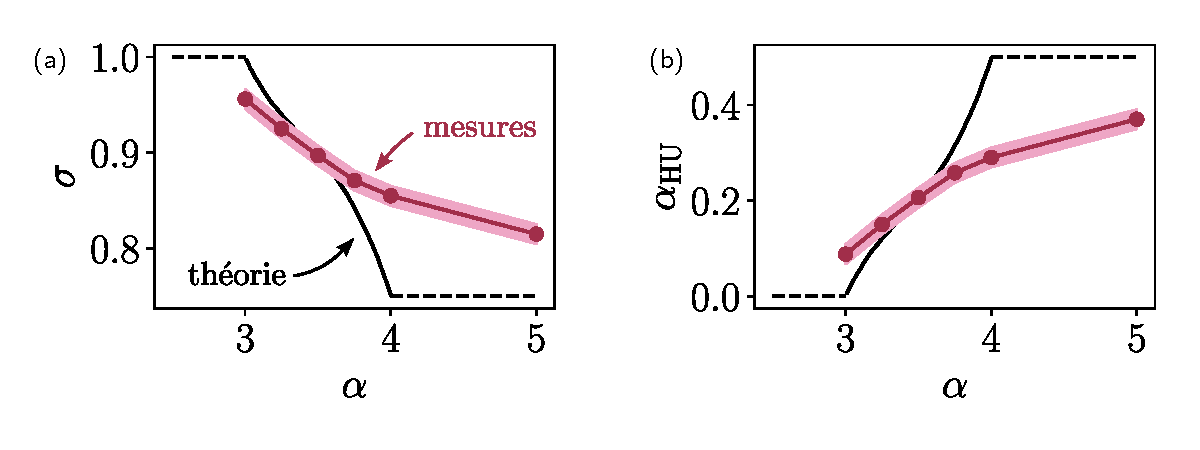
\includegraphics[width=0.9\textwidth]{Chapitre2/Figures/Hyperuniformity/eta_alpha_jumps.pdf}
	\caption{(a) Évolution de l'exposant d'hyperuniformité $\sigma$ avec la portée dans les modèles LR-ROM. La courbe noire représente les prédictions théoriques \cite{wiese_hyperuniformity_2024, wiese_theory_2022, wiese_longrange}. Les zones colorées rose représentent les incertitudes de détermination. (b) Déduction de l'évolution de l'exposant $\alpha_\text{HU}$ se basant sur l'\autoref{eq:eqsigmaalphahu}.}
	\label{fig:ExpTBLRJHU}
\end{figure}

\subsection{Difficultés dans les mesures d'hyperuniformité}

\subsubsection{Importance de la conservation du centre de masse}

\subparagraph{}Une première explication à ces différences vient du mouvement du centre de masse du système. En effet, dans la théorie de champ associée à CDP permettant d'effectuer les prédictions pour $\sigma$ présentées précédemment, le centre de masse du système est une quantité conservée \cite{wiese_blabla}. Or dans le LR-ROM, les sauts aléatoires des particules actives ne conservent ce centre de masse qu'en moyenne, leur direction étant complètement aléatoire. La rupture de cette symétrie fondamentale, directement reliée à la répartition des particules dans le système, pourrait donc affecter nos mesures de l'hyperuniformité et expliquer un désaccord avec les prédictions du cadre LR-CDP.

\subparagraph{}La façon la plus simple de le remarquer est de se placer dans le cas de la courte portée. Prenons le modèle Manna, appartenant à la classe CDP, et considérons deux de ses représentations. Dans la première représentation du modèle, l'implémentation est faite de la manière décrite à la \autoref{sec:ImplementationManna}, i.e. avec une redistribution aléatoire des particules sur les sites voisins. Celle-ci ne conserve donc pas le centre de masse du système. Dans la seconde représentation, lorsqu'un site est actif, il redistribue aléatoirement (i.e. dans une des deux directions du plan) une paire de particules sur deux sites voisins opposés, de manière à conserver le centre de masse du système à chaque instant. En effectuant alors des mesures sur ces deux représentations dans des configurations équivalentes avec $L=4096$ et $\langle A \rangle \approx 2\times 10^{-3}$, nous obtenons les résultats présentés à la \autoref{fig:HUCM}-(a)-(b).

\begin{figure}[h]
	\centering
	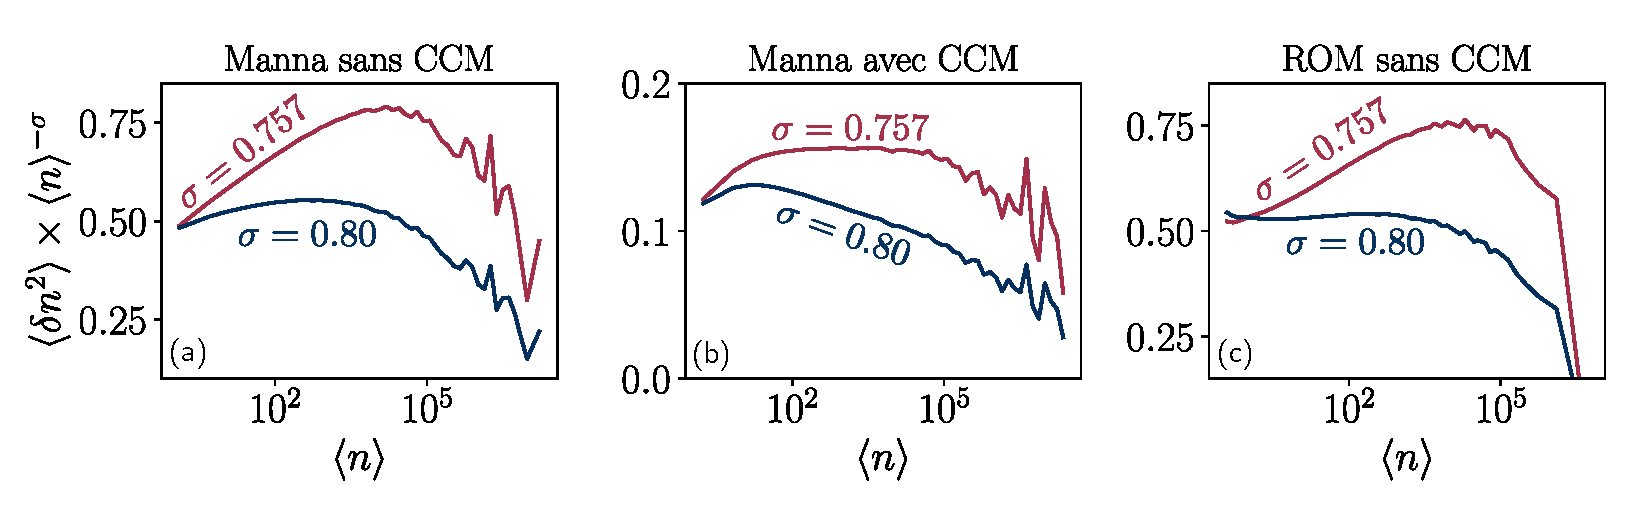
\includegraphics[width=\textwidth]{Chapitre2/Figures/Hyperuniformity/ImportanceCMHU.pdf}
	\caption{Représentation compensée de l'évolution de $\langle \delta n^2 \rangle$ avec $\langle n \rangle$ par une loi de puissance test dans (a) le modèle Manna sans conservation de la position du centre de masse ($\phi = 1.30628$), (b) le modèle Manna avec conservation de la position du centre de masse ($\phi = 1.75895$) et (c) le ROM ($\phi = 0.235248$). Les courbes rouges représentent la compensation par l'exposant test $\sigma = 0.757$, adéquate pour le modèle conservant la position du centre de masse, et les courbes bleues représentent la compensation par l'exposant test $\sigma = 0.80$, adéquat pour les modèles ne conservant pas la position du centre de masse.}
	\label{fig:HUCM}
\end{figure}

\subparagraph{}En représentant l'évolution $\langle \delta n^2 \rangle = f(\langle n \rangle)$ compensée par une loi test\footnote{Cette méthode de mesure est similaire à celle de la dérivée logarithmique mais permet de travailler avec des signaux plus bruités} $\langle n \rangle^\sigma$, ces mesures nous permettent d'estimer deux exposants distincts pour chacune des représentations : $\sigma \approx 0.76$ dans le cas où le centre de masse est conservé et $\sigma\approx 0.80$ dans le cas où il ne l'est pas. Dans le cas du ROM (donc avec des sauts courts) sans conservation du centre de masse, nous mesurons aussi dans ces mêmes conditions $\sigma\approx 0.80$, comme présenté à la \autoref{fig:HUCM}-(c).

\subparagraph{}Ces résultats suggèrent donc que la conservation du centre de masse joue un rôle essentiel dans les propriétés hyperuniformes du système. Notamment lorsque celle-ci est bafouée, il semble que cela revient à surestimer l'exposant $\sigma$ et donc diminuer l'hyperuniformité dans le système. Cela explique en partie pourquoi, dans le cas du LR-ROM, nous obtenons à $\alpha = 4$ une mesure de $\sigma\approx 0.86$ significativement plus grande que la valeur attendue $\sigma= 0.75$. Toutefois, cette valeur reste encore relativement éloignée de la valeur $\sigma\approx 0.80$ obtenue ici dans la limite de courte portée. Une explication à cette différence subsistante pourrait venir de la taille finie des systèmes étudiés.

\subsubsection{Effet de taille finie}

\subparagraph{}Si la loi de distribution des sauts des particules actives est une loi de puissance parfaite grâce à notre méthode de génération, en pratique elle se retrouve modifiée par sa mise en place dans un système de taille finie. En effet, par application des conditions aux limites périodiques, tous les sauts de taille $\Delta \gtrsim L$ se voient "repliés" dans l'espace périodique, changeant ainsi la distribution effective des sauts des particules actives. De plus, cette loi algébrique n'est définie que pour $\Delta>1$, du fait de l'introduction d'une distance de saut minimale lors de l'implémentation numérique.

\subparagraph{}Dans les approches théoriques permettant la prédiction de l'exposant $\sigma$, l'interaction à longue portée est considérée dans l'espace réciproque \cite{wiese_longrange}. Dans l'hypothétique système parfait et infini sur lequel se basent ces prédictions, la transformée de Fourier de la distribution de taille des sauts est définie par :

\begin{equation}
	\hat{P}_\Delta(q) \sim 1-|q|^{D-\alpha}
\end{equation}

\noindent soit correspondant à la fonction caractéristique d'une loi stable $S_{D-\alpha}$ dans la limite de petit $q$\footnote{Dans le cas d'une loi stable $S_{D-\alpha}$ on a en effet $\hat{P}_\Delta(q) \sim \text{exp}\left( -|q|^{D-\alpha} \right)$}. Une hypothèse est alors que dans nos simulations, dû à la taille finie du système et à l'introduction d'un cut-off, les distributions s'éloignent de cet attendu par l'addition de termes réguliers dans le développement de la fonction caractéristique :

\begin{equation}
	\hat{P}_\Delta(q) \sim 1-|q|^{D-\alpha} + q^2 + ...
	\label{eq:DevStable}
\end{equation}

\noindent Le premier terme régulier en $\sim q^2$ est sous-dominant pour $\alpha < D+2$. Cependant à mesure que $\alpha \rightarrow D+2$, soit $\alpha\rightarrow 4$ dans notre cas, cette sous-dominance n'est effective que dans un domaine de $q$ de plus en plus petits et donc des systèmes de tailles de plus en plus grandes. Ainsi, proche de $\alpha = 4$, on pourrait s'attendre à ce que la distribution de sauts effective s'écarte significativement la distribution utilisée dans la théorie\footnote{Après ça devrait l'écarter dans l'autre sens dans ce cas non ?}.

\begin{figure}[h]
	\centering
	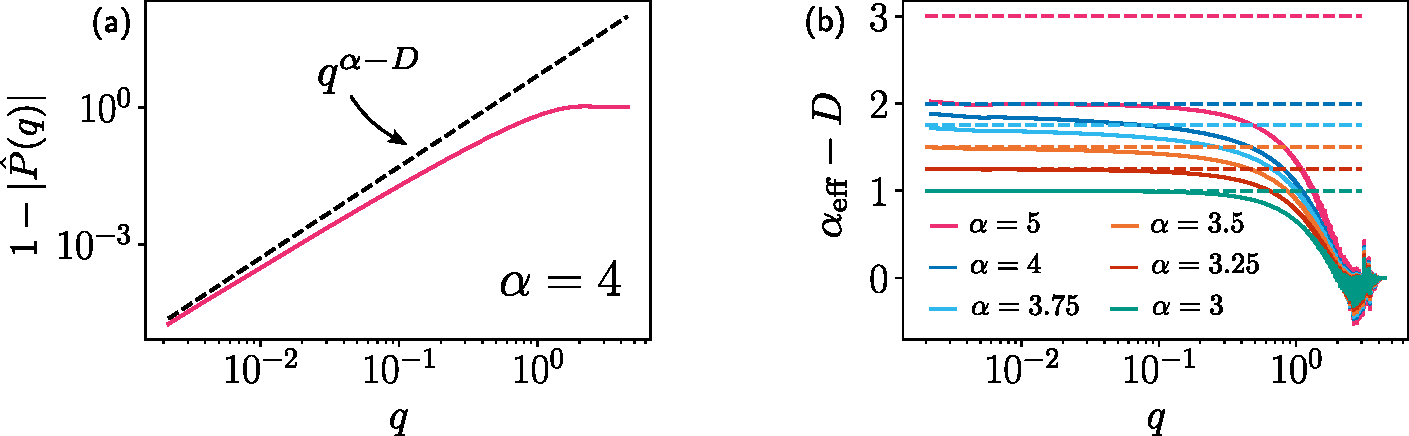
\includegraphics[width=\textwidth]{Chapitre2/Figures/Hyperuniformity/GammaEff_ROM.pdf}
	\caption{(a) Évolution de la quantité $1-|\hat{P}_\Delta (q)|$ avec $q$ pour le LR-ROM avec $\alpha=4$. En pointillé noir, le cas idéal sur lequel se basent les prédictions théoriques. (b) Exposant effectif obtenu par dérivée logarithmique de la courbe représentée en (a) pour toutes les portées $\alpha$. En pointillés de même couleur, la valeur $D-\alpha$ associée.}
	\label{fig:GammaEffROM}
\end{figure}

\subparagraph{}Pour le vérifier, nous considérons le cas du LR-ROM pour $L=4096$, dans lequel nous mesurons la distribution de probabilité $P(\mathbf{r})$ d'effectuer un déplacement $\mathbf{r}$ dans le système suite à un saut actif. En pratique nous en réalisons l'histogramme sur la grille introduite précédemment dans le cadre de la méthode cell-list. En prenant la transformée de Fourier discrète bidimensionnelle de cette distribution nous obtenons par une moyenne isotrope un équivalent de la distribution recherchée $\hat{P}_\Delta (q)$. Sur la \autoref{fig:GammaEffROM}, nous représentons $1-|\hat{P}_\Delta (q)|$ en fonction de $q$ pour $\alpha=4$ et la dérivée logarithmique obtenue de ces courbes pour chaque $\alpha$, définissant alors un exposant effectif local $\alpha_\text{eff}$. Pour chacune de ces portées, nous représentons en pointillés l'hypothèse théorique d'un exposant $\alpha-D$.

\subparagraph{}Nous observons alors effectivement une déviation de l'idéal théorique, d'autant plus que $\alpha$ se rapproche de $\alpha = 4$. De plus, pour $\alpha=5$, nous obtenons un exposant effectif $\alpha_\text{eff}\approx2$, signe de la prédominance du terme en $q^2$ dans l'\autoref{eq:DevStable} proposée précédemment, justifiant de ce fait notre raisonnement.
\`A la vue de ces observations, il est donc possible que les propriétés d'hyperuniformité du système soient effectivement affectées par les détails de l'implémentation des sauts à longue portée, et ce d'autant plus que $\alpha$ est proche de $\alpha=4$. Ceci, conjointement à la propriété de non-conservation de la position du centre de masse, pourrait expliquer le désaccord avec la théorie des résultats préliminaires obtenus dans le cas du LR-ROM.

%Afin de corriger cette dépendance, nous proposons une méthode de détermination d'un exposant de portée effectif $\alpha_\text{eff}$ équivalent à celui d'un système de taille infinie pour chaque portée $\alpha$. Cette méthode est bien sûr critiquable mais représente l'avancée actuelle de notre réflexion. Pour déterminer l'exposant effectif, nous opérons une moyenne logarithmique en fonction de $q$ de la dérivée logarithmique de $\hat{P}_\Delta(q)$ sur la zone $q<q_c$. Cette approche est motivée par la philosophie de calcul du groupe de renormalisation fonctionnel, dans laquelle chaque échelle de $q$ compte de manière équivalente. Le cut-off $q_c$ est alors choisi pour ignorer les effets de la dynamique microscopique du système. Pour ces mesures, nous faisons le choix arbitraire $q_c=xx$.
%
%\subparagraph{}Par cette méthode, il est possible d'associer à chaque portée $\alpha$ un exposant effectif $\alpha_\text{eff}$ permettant de resituer les résultats précédents. La courbe bleue sur la \textbf{Fig XX} montre alors les modifications apportées. Globalement, cette analyse permet de rationaliser en partie les écarts observés à courte portée, les associant à des exposants effectifs plus faibles. Toutefois, dans le cas du LR-ROM, la non conservation du centre de masse reste un élément de désaccord. Afin de conclure cette étude, nous proposons de poursuivre notre étude sur un modèle conservant la position de celui-ci.

\subsection{Hyperuniformité dans le modèle LR-Manna}

\subsubsection{Résultats préliminaires}

\subparagraph{}Pour aller un peu plus loin, nous proposons d'étudier l'hyperuniformité dans les modèles de transport à longue portée au plus proche possible des conditions d'applications des prédictions théoriques afin de les confronter directement. Pour ce faire, nous considérons le modèle LR-Manna dans sa version qui inclue la conservation de la position du centre de masse. Ce choix n'est pas anodin. Ce modèle étant plus simple que le LR-ROM, il est plus aisé dans ce cas de considérer des tailles de systèmes plus grandes, et ainsi se rapprocher de la limite théorique de système infini. Nous appliquons alors la méthode de box-counting sur des systèmes allant jusqu'à des tailles $L=16384$ et des distances au point critique allant jusqu'à $\delta\phi \approx 5\times 10^{-5}$ pour chaque portée $\alpha\in\{ 4, 3.75, 3.5, 3.25, 3 \}$. La \autoref{fig:MannaCMHU_gamma4} présente les résultats obtenus pour $\alpha = 4$ pour toutes les densités considérées.

\begin{figure}[h]
	\centering
	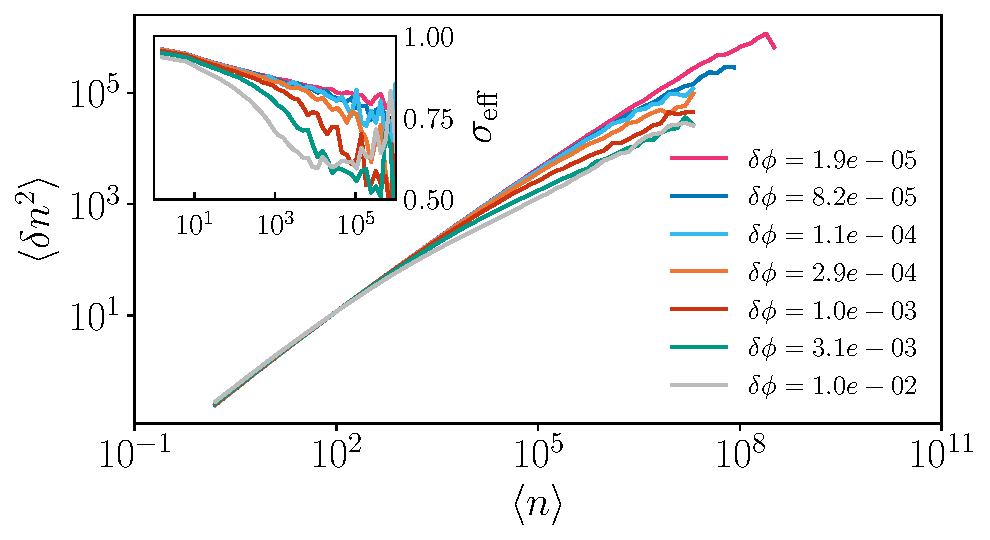
\includegraphics[width=0.9\textwidth]{Chapitre2/Figures/Hyperuniformity/MannaCM_gamma4_results.pdf}
	\caption{Évolution de $\langle \delta n^2 \rangle$ avec $\langle n \rangle$ dans le cas du modèle LR-Manna avec conservation de la position du centre de masse pour $\alpha=4$ à différentes distances $\delta\phi$ du point critique. En encart, l'évolution de l'exposant effectif mesuré par dérivation logarithmique des courbes en figure principale.}
	\label{fig:MannaCMHU_gamma4}
\end{figure}

\subparagraph{}Dans l'encart de cette figure, nous représentons l'exposant effectif local $\sigma_\text{eff}$ obtenu par dérivation logarithmique des courbes en figure principale. De manière assez surprenante, celui-ci semble évoluer de manière significative avec l'échelle de longueur considérée. Plus précisément, cette dépendance avec $\langle n \rangle$ semble être presque logarithmique, voire une loi de puissance de très faible exposant, jusqu'à un cut-off dépendant de la distance au point critique $\delta\phi$. Plus le système est proche du point critique, plus cette décroissance s'étend sur une large gamme d'échelles de longueur. Pour la distance la plus proche du point critique étudiée $\delta\phi\approx 2\times 10^{-5}$, il semblerait que cette évolution commence tout juste à arriver à saturation à grande échelle (léger début d'inflexion de la courbe) avant l'apparition du cut-off, suggérant le début d'une convergence vers la valeur asymptotique $\sigma$ de la limite thermodynamique de grande échelle.

\subparagraph{}Cette analyse des données préliminaires ne permet donc pas la mesure d'un exposant unique dans la limite de grande échelle et suggère qu'une meilleure approche du point critique est nécessaire pour cela. Les modèles Manna et ROM étant dans la même classe d'universalité, nous pouvons considérer qu'il en est en fait de même pour les données présentées à la \autoref{fig:ExpTBLRJHU}. Ceci expliquerait une partie du désaccord avec la prédiction théorique, notamment le fait que pour $\alpha=4$, nos mesures ne convergent pas vers celles obtenues à courte portée.

\subparagraph{}Dans le cadre du modèle LR-Manna, en prenant l'exemple de la portée $\alpha=4$ et en considérant qu'à taille de système infinie nous attendons $\sigma=0.75$, l'analyse de ces données suggère que le régime algébrique est atteint, pour un système infini, pour $\langle n \rangle^* \gg 2\times 10^7$ soit $l^* \gg 4\times 10^3$. Afin de le mesurer directement, il faut donc parvenir à sonder un état pour lequel la longueur de corrélation $\xi$ associée est telle que $\xi\gg l^*$. Or, avec les ressources actuellement à notre disposition, nous pouvons difficilement envisager des tailles de systèmes $L>16384$ et donc atteindre une telle longueur de corrélation sans tomber dans un état absorbant. 

\subparagraph{}Dans le cas des plus grandes portées $\alpha<4$, l'analyse est parfois un peu moins défavorable (essentiellement pour le cas $\alpha = 3$) mais conserve les mêmes conclusions. Dans la suite, en nous basant sur ces observations préliminaires, nous proposons une piste permettant une estimation de l'exposant d'hyperuniformité $\sigma$ de la limite thermodynamique à chaque portée, ou à défaut une borne supérieure raisonnable de son encadrement.

\subsubsection{Perspectives}

\subparagraph{}Comme nous l'avons présenté précédemment, une manière de mesurer efficacement l'hyperuniformité dans un système est de procéder à une méthode de redimensionnement par la distance au point critique. En suivant \cite{hexner_hyperuniformity_2015}, nous redimensionnons donc la dimension de la boîte de comptage $l$ par $\delta\phi^{-\nu_\perp^*}$, $\nu_\perp^*$ étant l'exposant de corrélation spatiale dérivé précédemment de la relation d'hyperscaling. Cela revient alors à redimensionner $\langle n \rangle_l$ par $\delta\phi^{-D \nu_\perp^*} = \delta\phi^{-2\beta-\gamma^\prime}$. Parallèlement, nous redimensionnons $\langle \delta n^2 \rangle$ par $\delta\phi^a$ avec $a$ un exposant test afin d'espérer une superposition des courbes sur une courbe maîtresse. Ce faisant, il n'est en pratique pas aisé de déterminer un critère de bonne superposition puisque cette dernière n'est possible que localement. Pour s'en apercevoir, un exemple de redimensionnement pour $\alpha=4$ est donné sur la \autoref{fig:MannaCMHU_rescale_gamma4}-(a), dans lequel nous avons essayé de superposer la région à grand $\langle n \rangle$. Une méthode de cette nature ne semble donc pas pouvoir nous informer davantage.

\subparagraph{}Toutefois, si nous opérons la même procédure sur l'exposant effectif (i.e. la dérivée logarithmique de ces courbes), il est possible de superposer toutes ses évolutions sur une courbe maîtresse. Un exemple est donné dans le cas $\alpha=4$ sur la \autoref{fig:MannaCMHU_rescale_gamma4}-(b) et le cas des autres portées est relégué à la \autoref{sec:mesures_HU_Manna}. De cette façon, il est possible d'en déduire précisément l'évolution algébrique de $\sigma_\text{eff}$ avec $\langle n \rangle$. Par ailleurs, nous remarquons que pour les distances $\delta\phi$ les plus petites, les courbes semblent s'éloigner légèrement, en moyenne, de cette superposition\footnote{Cette observation reste discutable du fait du bruit présent sur ces données préliminaires}. Cet écart correspondrait alors au début de saturation vers l'exposant asymptotique déjà suggéré sur les données brutes. En d'autres termes, il semblerait que l'exposant effectif suive une évolution du type :

\begin{equation}
	\sigma_\text{eff}  = \left( \sigma + \langle n \rangle^{-x} \right)g\left( \frac {\langle n \rangle }{\langle n \rangle_c} \right), \quad \langle n \rangle_c \sim \delta\phi^{-D\nu_\perp}
	\label{eq:esposantHULoi}
\end{equation}

\noindent avec $g$ une fonction à décroissance rapide. En pratique nous mesurons un exposant $x < 0.015$, décroissant davantage avec l'augmentation de la portée de l'interaction et donc la diminution de $\alpha$. $\alpha=4$ constitue donc le cas de plus forte dépendance de $\sigma_\text{eff}$ avec $\langle n \rangle$ même si celle-ci reste très ténue. 

\begin{figure}[h]
	\centering
	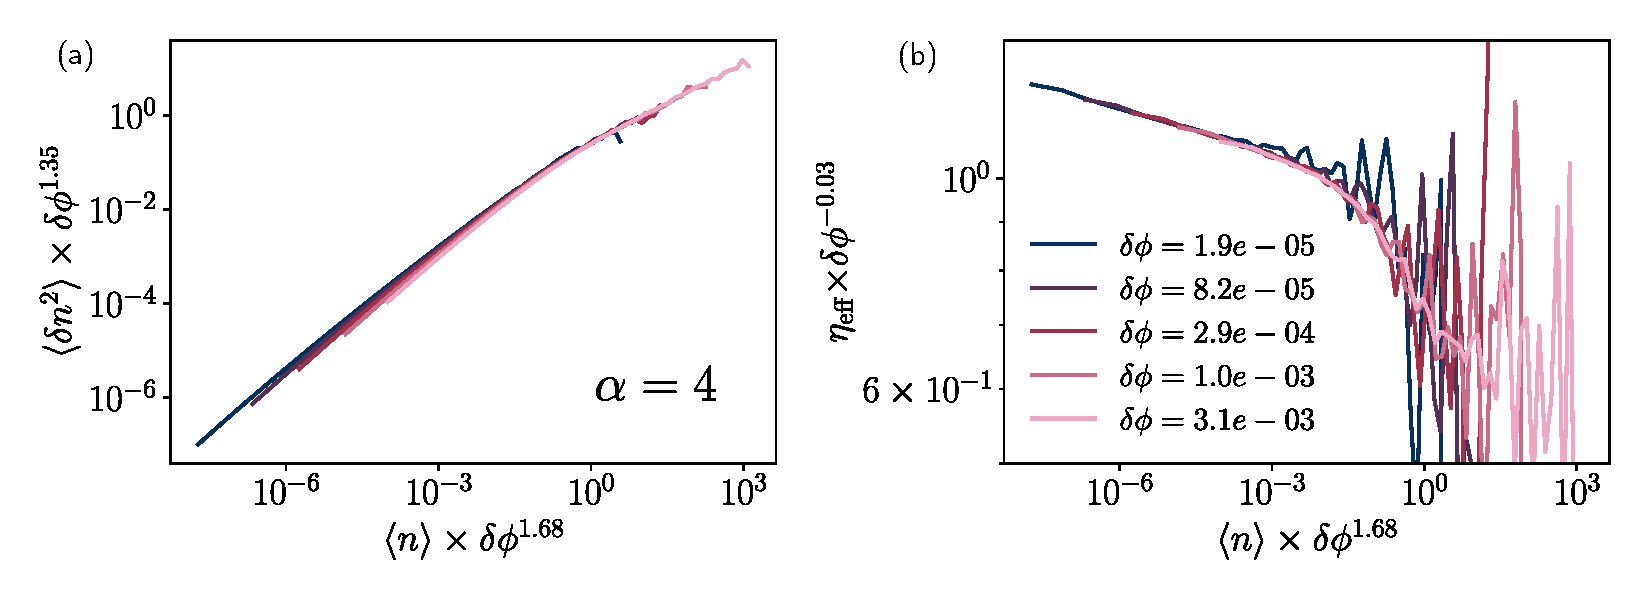
\includegraphics[width=\textwidth]{Chapitre2/Figures/Hyperuniformity/RescaleHU_MannaCM_Gamma4.pdf}
	\caption{Redimensionnement des mesures d'hyperuniformité dans le cas du modèle LR-Manna avec conservation de la position du centre de masse pour $\alpha=4$. Le redimensionnement par la distance au point critique $\delta\phi$ est appliqué sur (a) les données brutes et (b) l'exposant effectif obtenu par dérivée logarithmique.}
	\label{fig:MannaCMHU_rescale_gamma4}
\end{figure}

\subparagraph{}Cette méthode d'analyse, si elle ne nous permet pas de conclure sur la base de ces données préliminaires, présente un grand avantage : elle permet de déterminer sur une courbe $\langle  \delta n^2 \rangle  = f(\langle n \rangle )$ donnée la zone affectée par la distance finie au point critique considérée (i.e. l'influence du cut-off). Elle permet donc, si la forme donnée à l'\autoref{eq:esposantHULoi} est valide, de déterminer une borne supérieure sur l'encadrement de $\sigma$. En effet, dans ce cadre, tous les points sur la décroissance purement algébrique vérifient $\sigma_\text{eff}>\sigma$. Par ailleurs dans le cas le plus favorable $\alpha=3$ où la saturation vers l'exposant asymptotique semble être atteinte, nous pouvons estimer une valeur de $\sigma$, voire même une borne inférieure de l'encadrement. Ainsi, ces données préliminaires nous permettent de placer des indications de comparaison à la théorie sur la \autoref{eq:HUMannaShlag}. L'affinage nécessaire de ces estimations exige cependant un effort ultérieur.

\begin{figure}[h]
\centering
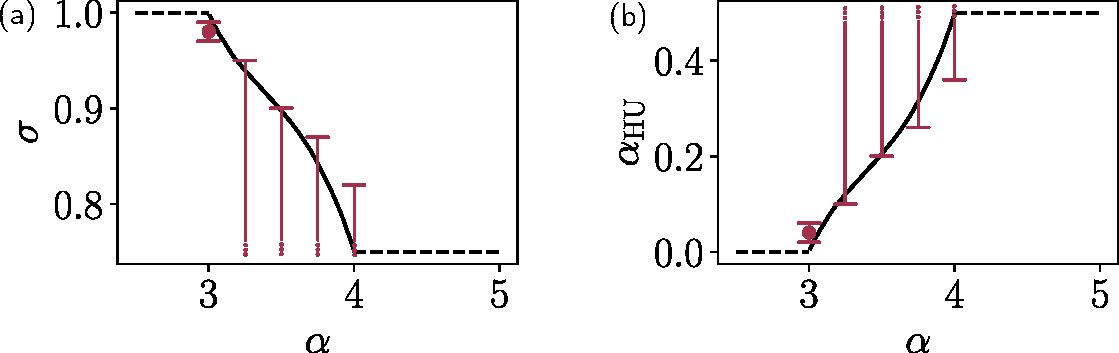
\includegraphics[width=0.8\textwidth]{Chapitre2/Figures/Hyperuniformity/eta_alpha_jumpsManna.pdf}
\caption{(a) Estimation de l'exposant d'hyperuniformité $\sigma$ dans le modèle LR-Manna avec conservation de la position du centre de masse pour les différentes portées $\alpha$. En pratique, il n'est possible d'encadrer et d'estimer la valeur de $\sigma$ que pour $\alpha=3$. Pour $\alpha>3$, nous proposons tout de même une borne supérieure de l'encadrement de cet exposant. En trait noir, les prédictions issues du mapping sur la transition de dépiégeage \cite{wiese_longrange}. (b) Déduction de l'évolution de l'exposant $\alpha_\text{HU}$ se basant sur l'\autoref{eq:eqsigmaalphahu}.}
\label{eq:HUMannaShlag}
\end{figure}

\subparagraph{}La détermination des propriétés hyperuniformes dans les modèles de sauts à longue portée exige donc de se placer à de très grandes échelles de longueur et donc des densités très proches du point critique. Il semble alors que c'est cette observation, plus que celle de la taille finie du système, ajoutée à celle concernant l'influence de la conservation du centre de masse, qui explique pourquoi nos mesures préliminaires dans le cadre du LR-ROM s'éloignent des prédictions théoriques. 

\subparagraph{}En conclusion, cette étude préliminaire révèle que les mesures de l'hyperuniformité dans ces modèles semblent relever d'une tâche très exigeante. La caractérisation quantitative des exposants $\sigma$ et leur évolution précise avec la portée $\alpha$ n'étant pas essentielles au reste de notre propos, nous nous limiterons à cette détermination au premier ordre. Celle-ci décrit alors, comme prédit par la théorie, une perte progressive de l'hyperuniformité dans le système avec l'augmentation de la portée de $\alpha=4$ à $\alpha=3$. La disparition de l'hyperuniformité pouvant être interprétée comme la disparition des corrélations spatiales de densité, cette observation est cohérent avec le fait que l'on rejoint un régime de champ moyen pour $\alpha <3$ dans le cadre LR-CDP. Ces éléments nous suffiront à contraster les évolutions observées en présence d'interactions médiées à longue portée dans les transitions de réversibilité et d'écoulement.

\subsubsection{Retour sur les exposants critiques}

\subparagraph{}La nécessité de s'approcher extrêmement près du point critique pour observer la criticalité de la limite thermodynamique pourrait aussi avoir un impact sur la détermination des exposants critiques présentée à la \autoref{sec:expcritjumps}. Cela pourrait expliquer pourquoi dans le cas identifié comme le plus défavorable $\alpha=4$, nous observons un écart à la limite de courte portée concernant les exposants $\beta$, $\gamma^\prime$ et $\delta$.

\subparagraph{}Toutefois, cette dépendance n'est pas évidente dans ces cas. En effet, sous un choix adéquat de densité critique $\phi_c$, les différentes lois de puissance déterminées sont bien plus convaincantes que celles obtenues par la méthode de box-counting dans le cadre de la mesure de l'hyperuniformité. Nous pouvons supposer par ailleurs que la conservation ou non de la position du centre de masse joue un rôle moins important dans le cas des exposants liés à l'activité dans le système ($\beta$, $\gamma^\prime$, $\delta$) plutôt qu'à la répartition de la masse ($\sigma$). Pour étudier ces hypothèses, il faudrait notamment sonder des états plus proches du point critique, requérant de fait une mobilisation de ressources numériques très importantes. Le but de ce travail étant essentiellement de caractériser une base de comparaison pour les études suivantes, nous nous limiterons aussi pour ces exposants à cette détermination de première ordre, tout de même relativement convaincante.

\section{Conclusion de chapitre}

\subparagraph{}Dans ce chapitre, nous avons défini le cadre théorique LR-CDP, représentant la présence d'un transport à longue portée induit localement par l'activité dans la classe CDP. Par une analyse d'échelle et des résultats pré-existants, nous avons prédit dans ce cadre l'évolution de la criticalité avec la portée des interactions $\alpha$. Notamment, en 2D, celle-ci prend place entre $\alpha=4$ et $\alpha=3$.


\subparagraph{}Pour préciser ce cadre, nous avons ensuite étudié des modèles emblématiques de la classe CDP auxquels nous avons ajouté un mécanisme de transport à longue portée. En caractérisant les transitions de phase absorbante associées à chaque portée de transport, nous avons montré que les exposants critiques évoluent continûment avec la portée du transport, allant de leur équivalent de courte portée à leur équivalent de champ moyen. Au premier ordre, cette évolution se fait dans la gamme de portées effectivement prédite par la théorie LR-CDP.

\subparagraph{}Dans une seconde partie, nous avons présenté une étude préliminaire des propriétés d'hyperuniformité de ces systèmes et leur évolution avec la portée du transport. La détermination des exposants critiques dans ce cadre s'est alors révélée bien plus compliquée, révélant un écart avec les prédictions théoriques dont nous avons proposé deux explications complémentaires. La première vient de la conservation de la position du centre de masse qui est essentielle à la correspondance aux prédictions théoriques. La seconde vient d'un comportement pré-asymptotique s'étendant sur de très grandes plages d'échelles de longueur, rendant difficile l'estimation du comportement dans la limite thermodynamique.

\subparagraph{}En conclusion, cette étude nous a permis de préciser la zone flottante d'évolution des exposants critiques située entre $\alpha=3$ et $\alpha = 4$ en deux dimensions. Grâce à cet ajout, nous disposons d'un cadre mieux défini pour décrire l'évolution de la criticalité des systèmes sous l'ajout d'un transport à longue portée. Dans la suite de cet thèse, nous nous servirons de cette base de comparaison afin de montrer que les interactions à longue portée, lorsqu'elles correspondent à des interactions médiées par le milieu non équivalentes à un transport, font évoluer la criticalité des systèmes d'une manière tout à fait différente.

\chapter{Transition de réversibilité dans les suspensions cisaillées cycliquement}

\label{chapter:Susp}

\subparagraph{}Dans le \autoref{chapter:introduction} nous avons vu que, sous cisaillement cyclique, les suspensions peuvent être soumises à une transition de réversibilité. Celle-ci peut être interprêtée comme une transition de phase absorbante \cite{pine_chaos_2005, corte_random_2008, tjhung_criticality_2016, ge_rheology_2022}. Le paramètre de contrôle de cette transition est alors l'amplitude de cisaillement appliquée $\gamma_0$ et le paramètre d'ordre le coefficient de diffusion stroboscopique des particules $D_0$. Dans la phase absorbante, pour $\gamma_0 < \gamma_{0,c}$, les particules de la suspension suivent un mouvement réversible, caractérisé par $D_0 = 0$. Dans la phase active, pour $\gamma_0 > \gamma_{0,c}$, les interactions irréversibles entre particules induisent une diffusion stroboscopique des particules d'un cycle à l'autre, caractérisée par $D_0 >0$. Proche de la transition ($\gamma_0\approx\gamma_{0,c}$), $D_0$, ses fluctuations $\langle \delta D_0^2 \rangle$ et la longueur de corrélation associée au système suivent une évolution dictée par les exposants critiques $\beta$, $\gamma^\prime$ et $\nu_\perp$ : 

\begin{equation}
	D_0 \sim \delta\gamma_0^\beta, \quad \langle \delta D_0^2 \rangle \sim \delta\gamma_0^{-\gamma^\prime},\quad \xi \sim \delta\gamma_0^{-\nu_\perp}, \quad \delta\gamma_0 = \frac{\gamma_0-\gamma_{0,c}}{\gamma_{0,c}}
\end{equation}

\subparagraph{}Les modélisations simples de ce système \cite{corte_random_2008, tjhung_criticality_2016, ge_rheology_2022} semblent placer ce phénomène critique dans la classe d'universalité CDP. Toutefois, en considérant les interactions entre les particules, médiées par le fluide suspendant, Mari et al. \cite{mari_absorbing_2022} ont proposé un modèle présentant une criticalité très différente. Alors que pour la classe CDP l'évolution du paramètre d'ordre est concave ($\beta < 1$) et ses fluctuations divergentes ($\gamma^\prime>0$), le modèle prenant en compte les interactions médiées définit une évolution convexe du paramètre d'ordre ($\beta >1$) et des fluctuations qui s'annulent au point critique ($\gamma^\prime < 0$).

\subparagraph{}Dans le \autoref{chapter:TransportLP}, nous avons vu que l'introduction de la longue portée sous forme de transport à longue portée dans un modèle appartenant à la classe CDP permettait de passer continûment de la criticalité de courte portée à celle de champ moyen. Cette évolution canonique suit un cadre théorique que nous avons appelé LR-CDP. Dans ce cas, nous avons sur toute cette gamme $\beta \leq 1$ et $\gamma^\prime \geq 0$. La criticalité exposée par le modèle prenant en compte les interactions médiées semble donc échapper à ce cadre.

\subparagraph{}Dans ce chapitre, nous proposons d'étudier plus en profondeur le modèle proposé par Mari et al. \cite{mari_absorbing_2022} afin de comprendre comment les interactions médiées à longue portée induisent une criticalité différente de celle induite par le transport à longue portée. Pour ce faire, nous présenterons un modèle numérique capable de prendre en compte ces interactions de manière spatialisée dans le système. Nous étudierons alors le comportement critique associé à ce modèle et sa dépendence en portée de l'interaction d'un point de vue statique, dynamique et structurel. Nous proposerons enfin un cadre de description champ moyen pour interpréter les fortes différences de comportement critique observées entre ce modèle et le cadre de référence LR-CDP.

\section{Importance de la spatialisation des interactions}

\paragraph{Limite de l'approche champ moyen}

\subparagraph{}Dans leur modèle initial, Mari et al. \cite{mari_absorbing_2022} ont implémenté les interactions à longue portée médiées par le fluide d'un point de vue champ moyen. Les détails de cette implémentation seront donnés dans la section suivante. Dans cette approche, chaque particule est soumise à une interaction médiée moyenne\footnote{au sens de moyenne spatiale}, assimilée à une sorte de diffusion, qui dépend uniquement du nombre instantané de particules subissant une interaction de contact irréversible dans le système. En d'autres termes, peu importe la distance d'une particule à un évènement irréversible, l'impact de ce dernier sur elle reste le même. Via ce modèle en deux dimensions, les auteurs ont mené des analyses numériques permettant de déterminer précisément la valeur des exposants critiques associés au paramètre d'ordre :

\begin{equation}
	\beta \approx 1.85, \quad \gamma^\prime \approx -1.3 
\end{equation}

\noindent Cette approche simplificatrice met alors en évidence un mécanisme, la diffusion des particules via les interactions médiées, permettant de sortir du cadre de description LR-CDP. En effet, nous rappelons que pour celui-ci nous avons en champ moyen $\beta = 1$ et $\gamma^\prime = 0$. 

\subparagraph{}Toutefois, d'un point de vue de la modélisation d'un système réel, ce modèle présente des lacunes. Notamment, comme nous l'avons vu au \autoref{chapter:introduction}, les interactions médiées par un fluide visqueux sont en général fonction de la distance. Celles-ci sont représentées formellement par un propagateur hydrodynamique, présenté à la \autoref{sec:ref_interac_visc}, qui décroît comme :

\begin{equation}
	\mathcal{G}_{ij}(\mathbf{r} - \mathbf{r}^\prime) \sim \frac{1}{|\mathbf{r} - \mathbf{r}^\prime|^\alpha}
\end{equation}

\noindent à grande distance $|\mathbf{r} - \mathbf{r}^\prime|$ de la source de l'interaction. La question est alors de savoir si le comportement critique exotique exhibé par le modèle traitant les interactions médiées en champ moyen est effacé par une représentation spatialisée de celles-ci ou s'il persiste dans cette prise en compte plus proche de la réalité des interactions médiées.

\paragraph{Quelle portée étudier ?}

\subparagraph{}La première question à nous poser pour mener notre étude est donc de savoir quelle est la portée $\alpha$ pertinente pour modéliser un système réel. En fait, comme nous l'avons vu à la \autoref{sec:ref_interac_visc}, cela dépend fortement du dispositif considéré. Dans le cadre de la transition de réversibilité des suspensions cisaillées cycliquement, nous pouvons imaginer par exemple deux conditions expérimentales simples.

\subparagraph{}La première concerne le cisaillement d'une suspension dans un écoulement de Couette, à la manière de Pine et al. \cite{pine_chaos_2005}. Dans ce cas, à condition que l'écart entre les parois rigides cylindriques soit suffisamment grand devant le diamètre des particules, le propagateur hydrodynamique pertinent pour décrire le système est celui associé à un milieu infini en trois dimensions, pour lequel nous avons montré $\alpha = 1$ (voir la \autoref{sec:ref_interac_visc} et la \autoref{sec:Annexe_Interactions_Hydro}). En considérant que les interactions irréversibles de contact entre les paires de particules agissent comme un dipôle de force sur le fluide, la portée pertinente pour caractériser les interactions dans ce système 3D correspond donc à $\alpha = 1+1 =2$.

\subparagraph{}La seconde concerne le cisallement d'une suspension dans un espace fortement confiné entre des plaques rigides, rendant le problème quasi-2D. La transition de réversibilité a déjà été étudiée dans un dispositif proche de ces conditions \cite{guasto_hydrodynamic_2010}. Dans ce cas là, nous avons vu que le propagateur hydrodynamique décroît comme $\sim 1/r^2$ à grande distance dans le milieu bidimensionnel, soit $\alpha = 2$ \cite{diamant_hydrodynamic_2009}. Selon la même hypothèse que les interactions irréversibles de contact entre les paires de particules correspondent à la forme dipolaire de l'interaction, la portée pertinente pour caractériser ce système 2D est donc $\alpha = 3$.

\subparagraph{}Nous pouvons imaginer encore d'autres dispositifs, comme par exemple un confinement quasi-2D sur une interface libre \cite{farhadi_shear_induced_2017}. Ainsi, il ne semble pas y avoir une portée pertinente mais des portées pertinentes pour aborder le problème de la transition de réversibilité. Dans ce chapitre, nous proposons donc d'étudier un modèle mettant en jeu des interactions dont la portée $\alpha$ peut être variée librement. Son étude nous permettra alors de mieux comprendre l'influence des interactions médiées et de leur portée sur la criticalité de la transition associée, replaçant ainsi l'étude de Mari et al. \cite{mari_absorbing_2022} dans une image plus globale et pertinente pour l'étude des systèmes réels.

\section{Méthode}

\subparagraph{}Dans cette section, nous présentons le modèle, dérivé du modèle étudié dans \cite{mari_absorbing_2022}, que nous avons mis au point pour étudier la transition de réversibilité en présence d'interactions médiées à longue portée.

\subsection{Le ROM comme modèle de dynamique stroboscopique}

\subparagraph{}D'un point de vue numérique, la transition de réversibilité dans les suspensions cisaillées cycliquement peut être étudiée de différentes façons. Les approches les plus évidentes, i.e. les plus proches des expériences, sont celles de dynamique moléculaire. Dans les travaux de Ge et Elfring \cite{ge_rheology_2022} par exemple, des suspensions de quelques 500 particules ont été étudiées et montrent effectivement une transition de réversibilité. Néanmoins, ces simulations comportant de nombreux degrés de liberté en-dehors de la position des particules (forme du potentiel d'interaction, modélisation du solvant, ...), il est difficile d'étendre ce type d'étude à des systèmes plus grands. Cette condition est pourtant indispensable à l'étude des phénomènes critiques, puisque celle-ci n'est valable qu'à grande échelle. De plus d'un point de vue conceptuel, pour questionner les propriétés universelles de la transition, il est plus judicieux de considérer des modèles minimaux et ainsi plus généraux.

\subparagraph{}Pour remédier à ce problème, il est nécessaire de s'appuyer sur des modélisations simplificatrices, basées sur des aspects phénoménologiques essentiels du problème. Une approche possible, développée par Corte et al. \cite{corte_random_2008}, consiste à considérer la dynamique du système d'un point de vue stroboscopique. En d'autres termes, les cycles de cisaillement ne sont pas considérés dans leur ensemble mais seulement représentés par deux instants : leur début et leur fin (voir \autoref{fig:equivROMSusp}). Le postulat de modélisation est alors le suivant : lorsqu'au cours d'un cycle deux particules sont suffisamment rapprochées par le cisaillement, elles interagissent de manière irréversible. Cette interaction irréversible implique alors qu'entre le début et la fin du cycle, les particules ayant interagi ne se retrouvent pas exactement à la même position. L'irréversibilité des interactions que subissent les particules pouvant avoir des origines complexes \cite{drazer_microstructure_2004}, dans un but de simplification globale, l'approche stroboscopique considère ces interactions comme erratiques. En d'autres termes, d'un pas au suivant de la modélisation stroboscopique, les particules ayant interagi subissent un déplacement aléatoire de courte amplitude.

\subparagraph{}Le modèle simplifié recherché doit donc, à chaque pas de temps, déterminer la distance entre les particules en début de cycle. Celles suffisamment proches sont considérées comme interagissant durant le cycle et sont donc déplacées aléatoirement au prochain pas de temps, i.e. à l’issue de ce cycle. L'état réversible absorbant correspond dans ce cas à un état où toutes les particules de la suspension sont suffisamment éloignées pour ne pas interagir. L'état irréversible correspond au contraire à un état où, dans le régime stationnaire, il y a toujours des déplacements sur un pas de temps. Ce modèle correspond donc exactement au ROM, introduit et étudié dans les chapitres précédents, comme illustré à la \autoref{fig:equivROMSusp}. En réalité cette correspondance n'est pas un total hasard puisque le ROM a justement été créé pour modéliser cette transition \cite{corte_random_2008}.

\begin{figure}[h]
	\centering
	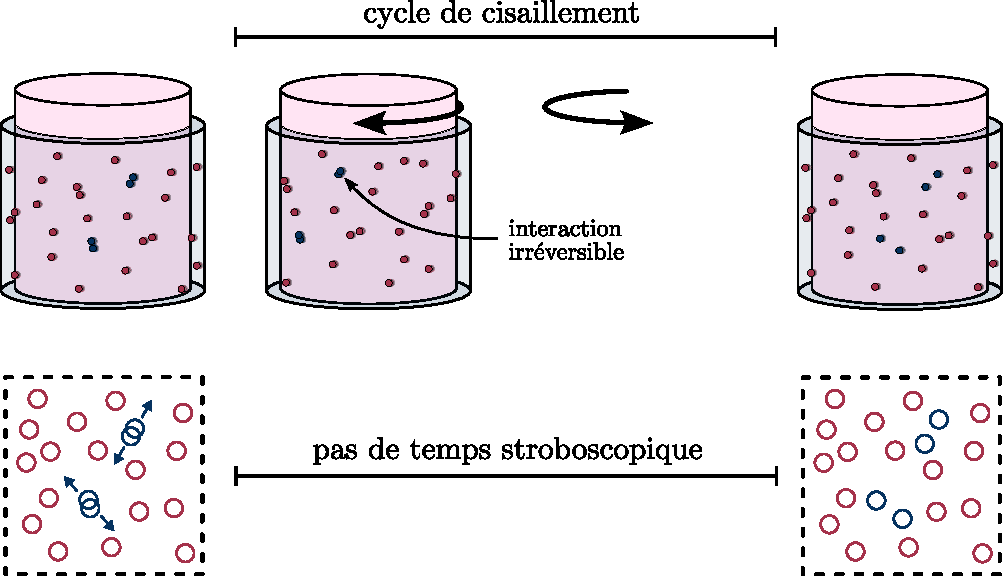
\includegraphics[width=0.85\textwidth]{Chapitre3/Figures/Method/equivROMSusp.pdf}
	\caption{Équivalence entre la vision dynamique et la vision stroboscopique dans les expériences de suspensions cisaillées cycliquement}
	\label{fig:equivROMSusp}
\end{figure}

\subparagraph{}Toutefois, nous avons vu dans le \autoref{chapter:introduction} que la transition de réversibilité était une transition de phase absorbante avec comme paramètre de contrôle l'amplitude de cisaillement $\gamma_0$ et comme paramètre d'ordre le coefficient de diffusion stroboscopique $D_0$. Il n'est donc pas évident de transposer ces observables au ROM, pour lequel le paramètre de contrôle est la densité de particules $\phi$  et le paramètre d'ordre l'activité $A$. En effet, dans le modèle stroboscopique, la notion de cisaillement est totalement perdue. Pourtant, il est possible de faire un parallèle entre ces deux approches. En fait, dans les expériences et simulations de la transition de réversibilité, l'amplitude de cisaillement critique $\gamma_{0,c}$ est fonction de la densité de particules $\phi$ dans le système. Par exemple dans les expériences de Pine et. al \cite{pine_chaos_2005} et les simulations de Ge et al. \cite{ge_rheology_2022}, il a été observé que $\gamma_{0,c}\sim \phi^{-D}$ comme le montrent les résultats présentés sur la \autoref{fig:phivsgamma}.

\begin{figure}[h]
	\centering
	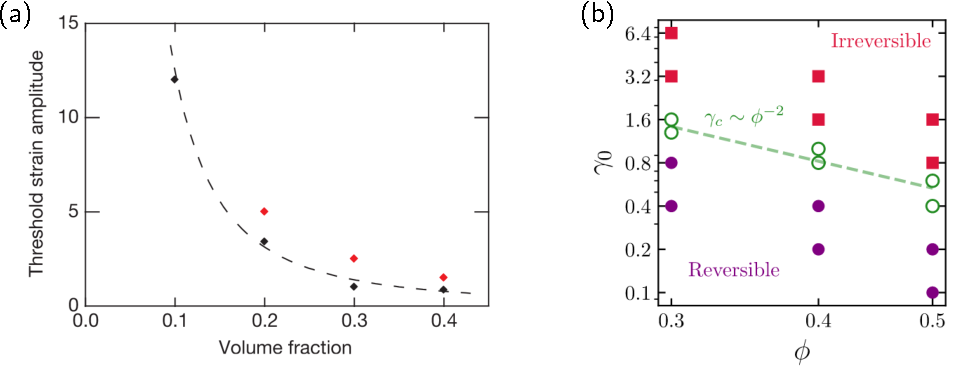
\includegraphics[width=0.9\textwidth]{Chapitre3/Figures/Method/phivsgamma.pdf}
	\caption{Diagrammes de phase des transitions de réversibilité dans les expériences de Pine et al. \cite{pine_chaos_2005} (a) et les simulations de Ge et al. \cite{ge_rheology_2022} (b) montrant l'évolution de l'amplitude de cisaillement critique $\gamma_{0,c}$ avec la densité de particules. Les lignes pointillées représentent la ligne de transition.}
	\label{fig:phivsgamma}
\end{figure}

\noindent Il est donc possible en pratique de passer de l'état absorbant à l'état diffusif en gardant l'amplitude de cisaillement $\gamma_0$ constante et en variant la densité de particule jusqu'à ce que celle-ci définisse $\gamma_{0,c}(\phi) = \gamma_0$. En d'autres termes, la densité de particules représente une autre variable que $\gamma_0$ permettant de traverser la ligne de transition, représentée sur la \autoref{fig:phivsgamma}. Ainsi, elle constitue aussi un paramètre de contrôle de cette transition expérimentale, ce qui permet donc de faire un lien direct avec la modélisation offerte par le ROM. De la même façon, le coefficient de diffusion stroboscopique du système réel est directement relié au nombre de particules interagissant irréversiblement. Ainsi, un paramètre d'ordre équivalent est bien l'activité dans le ROM. En d'autres termes, sous ce prisme, une particule active dans le ROM est une particule interagissant irréversiblement dans la vision dynamique. Par la correspondance $\gamma_0 \rightarrow \phi$ et $D_0\rightarrow A$, le ROM est donc le modèle numérique idéal pour simuler la transition de réversibilité dans les suspensions cisaillées cycliquement de par sa simplicité.

\subparagraph{}Suivant ces lignes, comme nous l'avons évoqué au \autoref{chapter:introduction}, Tjhung et al. \cite{tjhung_criticality_2016} ont utilisé cette équivalence pour justifier l'appartenance de cette transition à la classe CDP. Toutefois cette approche omet la présence attendue d'interactions hydrodynamiques entre les particules. Notre objectif est alors de comprendre comment ces interactions à longue portée peuvent affecter la criticalité du système. Or, si le ROM est un modèle efficace pour sonder la transition dans le cas d'interactions à courte portée, il ne permet pas en l'état de modéliser les interactions médiées par le fluide suspendant.

\subsection{Modélisation des interactions médiées}

\subparagraph{}Afin de conserver l'efficacité du modèle stroboscopique tout en y ajoutant la présence d'interactions médiées à longue portée, ces dernières doivent pouvoir être modélisées de manière simple et efficace. Le premier objectif de cette étude est donc de déterminer la modélisation adaptée.

\subparagraph{}En pratique, au cours d'un cycle de cisaillement, chaque particule suspendue dans le fluide interagit avec les autres particules via des interactions hydrodynamiques, dont la forme a été explicitée à la \autoref{sec:ref_interac_visc} et à la \autoref{sec:Annexe_Interactions_Hydro}. Celle-ci suppose un écoulement à bas Reylnolds régi par les équations de Stokes et des particules ponctuelles sans inertie. Une particule interagissant irréversiblement en $\mathbf{r}^\prime$ et appliquant une force $\mathbf{F}\delta(\mathbf{r}^\prime)$ sur le fluide induit une vitesse de déplacement $\mathbf{v}^p(\mathbf{r})$ pour une particule située en $\mathbf{r}$ selon\footnote{Nous utilisons ici la convention d'Einstein pour la sommation sur les indices répétés.} :

\begin{equation}
	v^p_i(\mathbf{r}) = \mathcal{G}_{ij}(\mathbf{r}-\mathbf{r}^\prime)F_j
\end{equation}

\noindent avec $\mathcal{G}_{ij}(\mathbf{r}-\mathbf{r}^\prime)$ le propagateur hydrodynamique adéquat pour la modélisation du problème, décroissant comme $1/|\mathbf{r}-\mathbf{r}^\prime|^\alpha$ à grande échelle, avec $\alpha$ dépendant de la géométrie considérée.

\subparagraph{}Au cours de la transition réelle, les déplacements irréversibles des particules et donc les forces qu'elles exercent lors d'un cycle prennent des formes complexes et ne sont a priori pas instantanés. Afin de modéliser simplement l'influence d'un tel évènement, nous le considérons donc simplement dans l'approche stroboscopique. Nous considérons alors que chaque particule active située en $\mathbf{r}^\prime$ effectue un déplacement aléatoire $\boldsymbol\delta^a(\mathbf{r}^\prime)$, qui induit un déplacement $\boldsymbol\delta^p(\mathbf{r})$ sur une particule située en $\mathbf{r}$ selon :

\begin{equation}
	\delta^p_i(\mathbf{r}) = \mathcal{G}_{ij}(\mathbf{r}-\mathbf{r}^\prime)\delta^a_j(\mathbf{r}^\prime)
\end{equation}

\noindent avec le même propagateur hydrodynamique.

\subparagraph{}Cette modélisation implique une approche tensorielle de l'influence des particules actives sur les particules passives (par opposition à actives) dans le modèle stroboscopique : le déplacement d'une particule passive induit par une particule active dépend de la direction de déplacement de cette dernière. Pour simplifier davantage cette approche, nous nous appuyons sur le fait que, dans la phase active, dans la limite thermodynamique, chaque particule passive reçoit des interactions médiées de la part d'un grand nombre particules actives. En notant $\{ \mathbf{r}^\prime \}$ l'ensemble des positions des particules actives, on a alors :

\begin{equation}
	\delta^p_i(\mathbf{r}) = \sum_{\mathbf{r}^\prime}\mathcal{G}_{ij}(\mathbf{r}-\mathbf{r}^\prime)\delta^a_j(\mathbf{r}^\prime)
\end{equation}

\noindent De ce fait, nous pouvons aborder cette interaction d'un point de vue statistique. Les déplacements des particules actives étant aléatoires et donc de moyenne nulle, on a de même $\langle \delta^p_i(\mathbf{r}) \rangle = 0$ avec $\langle \cdot \rangle$ représentant une moyenne sur les déplacements aléatoires des particules actives. En considérant les déplacements des particules actives décorrélés et d'amplitude typique $\sigma$, on a :

\begin{equation}
\begin{aligned}
	\langle\boldsymbol\delta^p(\mathbf{r})^2\rangle &= \sum_{\mathbf{r}^\prime}\sum_{\mathbf{r}^{\prime\prime}}\mathcal{G}_{i\alpha}(\mathbf{r}-\mathbf{r}^\prime)\mathcal{G}_{i\beta}(\mathbf{r}-\mathbf{r}^{\prime\prime})\langle\delta^a_\alpha(\mathbf{r}^\prime)\delta^a_\beta(\mathbf{r}^{\prime\prime})\rangle \\
	&= \sum_{\mathbf{r}^\prime}\sum_{\mathbf{r}^{\prime\prime}}\mathcal{G}_{i\alpha}(\mathbf{r}-\mathbf{r}^\prime)\mathcal{G}_{i\beta}(\mathbf{r}-\mathbf{r}^{\prime\prime})\sigma^2\delta_{\mathbf{r}^\prime\mathbf{r}^{\prime\prime}}\delta_{\alpha\beta}\\
	&= \sigma^2\sum_{\mathbf{r}^\prime}\mathcal{G}_{i\alpha}(\mathbf{r}-\mathbf{r}^\prime)\mathcal{G}_{i\beta}(\mathbf{r}-\mathbf{r}^{\prime})\delta_{\alpha\beta}\\
	&= \sigma^2 \sum_{\mathbf{r}^\prime}\mathcal{G}_{i\alpha}(\mathbf{r}-\mathbf{r}^\prime)\mathcal{G}_{i\alpha}(\mathbf{r}-\mathbf{r}^{\prime})
\end{aligned}
\end{equation}

\noindent les sommes sur les indices de coordonnées $i$ et $\alpha$ étant implicites. Nous considèrerons donc simplement dans notre modélisation statistique :

\begin{equation}
	\langle \boldsymbol\delta^p(\mathbf{r})^2 \rangle \sim \sigma^2 \sum_{\mathbf{r}^\prime} \mathcal{G}^2(\mathbf{r}-\mathbf{r}^\prime)
	\label{eq:convol_model}
\end{equation}

\noindent avec $\mathcal{G}$ un propagateur scalaire effectif de l'interaction, que nous choisissons isotrope et décroissant comme $1/r^{\alpha}$ de la même manière que le propagateur hydrodynamique tensoriel associé.

\subparagraph{}En pratique, Le propagateur scalaire effectif retenu pour la modélisation est de la forme spécifique suivante :

\begin{equation}
	\mathcal{G}^2(\mathbf{r}-\mathbf{r}^\prime) = \frac{c}{\left(1+\left(\frac{|\mathbf{r}-\mathbf{r}^\prime|}{D_p}\right)^2\right)^\alpha}, \quad c > 0
\end{equation}

\noindent avec $D_p$ le diamètre des particules et $c$ un paramètre représentant la borne supérieure de l'interaction. Cette formulation modélise alors bien une interaction entre particules actives et particules passives qui décroît comme $1/r^\alpha$ en champ lointain. La régularisation en $|\mathbf{r}-\mathbf{r}^\prime|=0$ permet par ailleurs de considérer sans difficulté des interactions pour lesquelles on a $2\alpha > D$, sans quoi cette forme ne serait plus intégrable. Pour $2\alpha < D$, la non-intégrabilité du propagateur en $|\mathbf{r}|\rightarrow\infty$ et sa prise en compte dans le modèle sera discutée à la \autoref{sec:noninteg}.

\subparagraph{}In fine, sous ce point de vue statistique, nous considérons que chaque particule passive effectue à chaque pas de temps stroboscopique un déplacement aléatoire gaussien de moyenne nulle et de variance donnée par l'\autoref{eq:convol_model}. Ces simplifications permettent alors de rendre la modélisation des interactions scalaire, ce qui permet d'alléger fortement l'implémentation numérique que nous détaillons dans la partie suivante.

\subsection{Implémentation numérique}

\subparagraph{}Pour l'implémentation numérique de ce modèle, nous reprenons les éléments de base du ROM, détaillé au \autoref{chapter:TransportLP}. Les interactions médiées représentent alors simplement une composante additionnelle à ce modèle, à implémenter à chaque pas de temps. 

\subsubsection{Calcul de l'influence des particules actives}

\subparagraph{}Afin de simplifier le calcul numérique de la somme de l'\autoref{eq:convol_model}, nous choisissons de considérer une version gros grains de l'activité dans le système. Pour ce faire, nous définissons un champ d'activité discret $A(\mathbf{r}_i)$, défini sur le réseau utilisé pour la méthode cell-list, introduite à la \autoref{sec:DetImpl}. Chaque case du réseau est alors définie autour d'une position $\mathbf{r}_i = na\hat{\mathbf{e}}_x + ma \hat{\mathbf{e}}_y$ avec $(n,m) \in \mathbb{N}^2$ et $a$ le pas du réseau que l'on prend de nouveau égal à $D_p=1$. \`A chaque pas de temps, après identification des particules actives, nous calculons ce champ d'activité sur la case du réseau centrée autour de $\mathbf{r}_i$ comme le nombre de particules actives dans cette case (voir \autoref{fig:modelsusp}). $A(\mathbf{r}_i)$ représente alors en quelque sorte une quantité d'activité locale.

\begin{figure}[h]
	\centering
	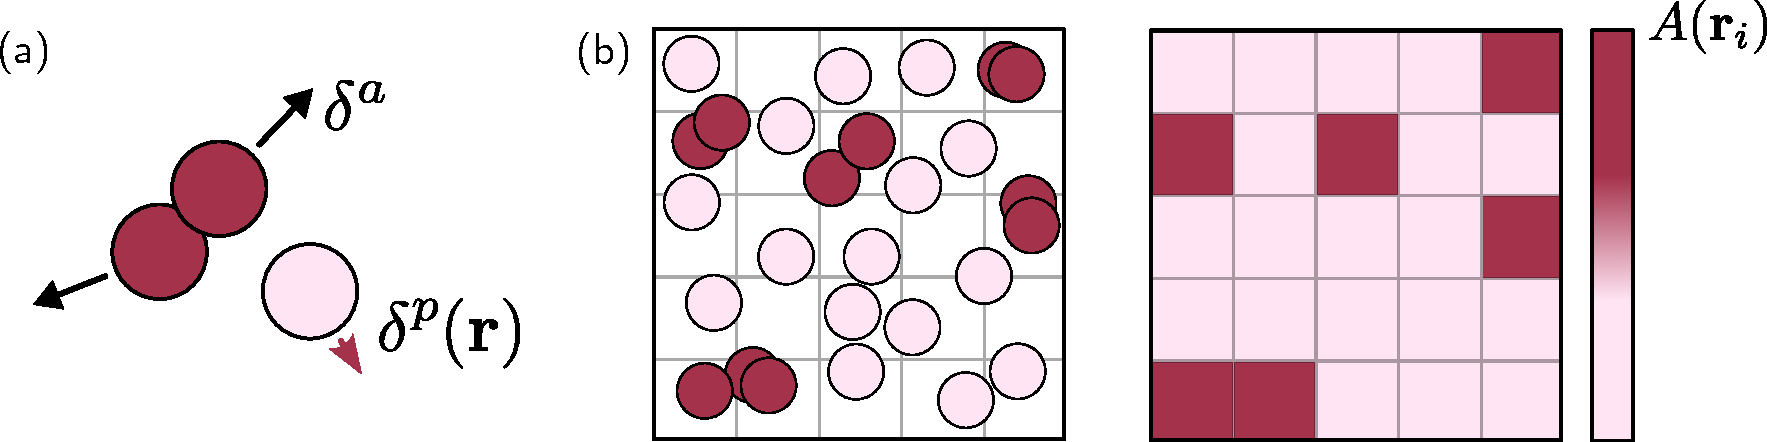
\includegraphics[width=0.9\textwidth]{Chapitre3/Figures/Method/Model.pdf}
	\caption{Implémentation numérique du modèle $\alpha$-ROM. (a) Les particules actives (rouges) sont soumises à des déplacements aléatoire $\boldsymbol\delta^a$ indépendants de leur position. Les particules passives sont soumises à des déplacements aléatoires $\boldsymbol\delta^p$ dont l'amplitude typique dépend de leur distance à l'activité. (b) Méthode de détermination du champ d'activité discret $A(\mathbf{r}_i)$.}
	\label{fig:modelsusp}
\end{figure}

\subparagraph{}Pour déterminer la variance du déplacement des particules passives à chaque pas de temps, il suffit donc de calculer la convolution discrète suivante :

\begin{equation}
	\langle \boldsymbol\delta^p(\mathbf{r}_i)^2\rangle = \sigma^2\sum_{j} G^2(\mathbf{r}_i-\mathbf{r}_j) A(\mathbf{r}_j)
	\label{eq:kick_discret}
\end{equation}

\noindent avec $G^2$ la version discrétisée du propagateur $\mathcal{G}^2$. Cette convolution étant définie sur un réseau régulier, il est possible de la calculer efficacement en passant par l'espace de Fourier. En pratique, nous la calculons donc dans l'espace réciproque où elle devient le simple produit $\hat{G^2}(\mathbf{q}_i)\hat{A}(\mathbf{q}_i)$, avec $\mathbf{q}_i = (\frac{2\pi}{L}n, \frac{2\pi}{L}m)$ et $L$ la taille du système. La notation $\hat{\cdot}$ définit alors ici la transformée de Fourier discrète sur ce réseau. Pour ce faire, nous définissons directement le propagateur hydrodynamique dans l'espace de Fourier. Dans le cas continu, le calcul relégué à la \autoref{sec:TFinverse_susp} donne en deux dimensions :

\begin{equation}
	\hat{\mathcal{G}^2}(\mathbf{q})=\frac{2\pi c}{\Gamma\left(\alpha\right)} \left( \frac{q}{2} \right)^{\alpha-1}K_{\alpha-1}(q)
	\label{eq:propcontinu2D}
\end{equation}

\noindent avec $\Gamma$ la fonction Gamma d'Euler et $K_{\alpha -1}$ la fonction de Bessel modifiée de seconde espèce d'ordre $\alpha - 1$ \cite{abramowitz_handbook_1965}. On peut alors estimer la valeur de ce propagateur continu en $\mathbf{q}=0$ pour un milieu de taille finie en calculant sa valeur moyenne dans l'espace réel :

\begin{equation}
	\hat{\mathcal{G}^2}(0) = \frac{\pi c}{\alpha -1}\left( 1- \left( 1+L^2 \right)^{1-\alpha} \right) \xrightarrow[L\rightarrow\infty]{\alpha > 1} \frac{\pi c}{\alpha - 1}
	\label{eq:zerovalue}
\end{equation}

\noindent Nous choisissons donc de définir le propagateur discret $\hat{G}$ dans l'espace réciproque via l'expression :

\begin{equation}
	\hat{G^2}(\mathbf{q}_i) = \hat{\mathcal{G}^2}(\mathbf{q}_i), \quad q = \sqrt{\left( 2-2\cos \left( \frac{2\pi}{L}n \right) \right) + \left( 2-2\cos \left( \frac{2\pi}{L}m \right) \right)}
\end{equation}

\noindent la conversion du nombre d'onde sous sa fomre discrète étant essentielle pour définir proprement le propagateur dans l'espace réciproque discret \cite{ferrero_criticality_2019, rossi_finite-disorder_2022}, comme nous l'expliquons dans la \autoref{sec:impl_disc_propag}.

\subparagraph{}Finalement, la valeur réelle de la convolution est obtenue en opérant une transformée de Fourier inverse discrète sur le produit. La forme alors obtenue par cette procédure pour $\alpha \in \{ 3, 2, 1.5 \}$ est présentée à la \autoref{fig:PropagTBLRR}-(a). Cette méthode de calcul de la convolution étant parallélisable, elle nous permet de conserver l'architecture GPU utilisée pour les simulations précédentes. De plus, la méthode pseudo-spectrale permet de prendre en compte les conditions aux limites périodiques du système naturellement. Enfin, afin d'optimiser notre utilisation des fonctions de Fast Fourier Transform \cite{cooley_algorithm_1965}, nous privilégions les tailles de système de la forme $L = 2^p$ avec $p \in \mathbb{N}$.

\subparagraph{}De cette manière, en plus des particules actives, les particules passives sont soumises à un déplacement dont la variance est donnée par l'\autoref{eq:kick_discret} à chaque pas de temps. Ce modèle représente alors une généralisation du modèle étudié par Mari et al. \cite{mari_absorbing_2022}. En effet, celui-ci correspond en fait exactement au cas $\alpha = 0$ (et donc des interactions médiées indépendantes de la distance) qui correspond bien à une limite champ moyen de la prise en compte des interactions hydrodynamiques.

\subparagraph{}L'ajout de ce nouveau mécanisme de diffusion des particules passives conserve la présence d'une transition de phase absorbante analogue à celle du ROM et dont les propriétés critiques varient avec la portée de l'interaction $\alpha$. Nous appelons alors ce nouveau modèle $\alpha$-ROM, et, par analogie, celui de Mari et al. 0-ROM. 

\subsubsection{Non-intégrabilité du propagateur à longue portée}

\label{sec:noninteg}

\subparagraph{}Si la régularisation du propagateur en $r=0$ permet de le rendre intégrable pour $2\alpha > D$, pour $2\alpha<D$ c'est la limite $r\rightarrow\infty$ qui pose problème. En effet, dans ce cas, la valeur moyenne du propagateur diverge comme $L^{2-2\alpha}$ pour $L$ grand. Si cette divergence n'est pas un problème en soi pour l'étude d'un système de taille finie, elle en représente un pour la comparaison des comportements critiques à différentes tailles. En effet, cette dépendance du propagateur en taille rend la densité critique $\phi_c$ elle aussi fortement dépendante de $L$ (voir \autoref{fig:PropagTBLRR}-(b)). De ce fait, il n'est alors plus possible d'utiliser différentes tailles du système pour sonder le comportement critique à une portée $\alpha$ donnée, comme cela a été fait à la \autoref{sec:expcritjumps} dans le cas des sauts à longue portée.

\subparagraph{}Afin de remédier à ce problème, nous choisissons de normaliser les propagateurs pour $2\alpha<D$ par un facteur $L^{2-2\alpha}$, rendant de ce fait la valeur moyenne du propagateur indépendante de la taille du système. Par cette procédure, nous retrouvons alors pour $\alpha = 0.5$ une densité critique indépendante de la taille du système à grande taille (voir \autoref{fig:PropagTBLRR}-(c)). Toutefois pour $\alpha = 1$, pour lequel la divergence de la valeur moyenne du propagateur évolue logarithmiquement avec la taille, cette procédure de normalisation par un facteur $\ln (L)$ n'est pas concluante. En effet, dans ce cas, $\phi_c$ montre une forte dépendance avec la taille du système même après normalisation. Ceci peut être expliqué par le fait qu'une telle divergence logarithmique n'est valable qu'à des tailles de systèmes excessivement grandes. Ce cas restant néanmoins d'intérêt, nous conservons son étude mais nous nous limitons pour cela à une taille de système fixée.

\begin{figure}[h]
	\centering
	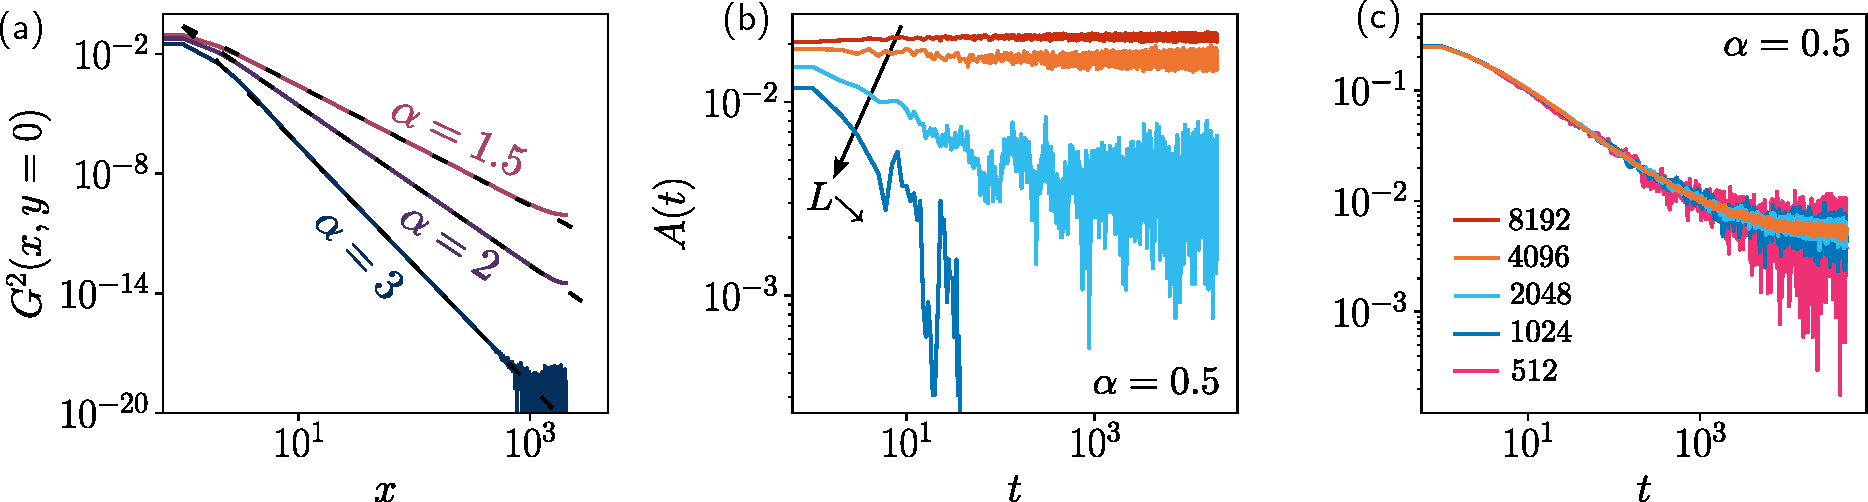
\includegraphics[width=\textwidth]{Chapitre3/Figures/Method/PropagTBLRR2D.pdf}
	\caption{Propagateurs d'interaction dans le modèle $\alpha$-ROM. (a) Évolution du propagateur effectif dans l'espace discret réel pour $\alpha \in \{ 3, 2, 1.5 \}$. Les pointillés noirs représentent les lois de puissance $1/r^{2\alpha}$. (b) Évolution de l'activité vers l'état stationnaire à $\phi = 0.00486859$ pour différentes tailles de système avec $\alpha = 0.5$ dans le cas d'un propagateur non normalisé. La distinction des courbes montre un point critique nettement différent pour chaque taille. (c) Idem à $\phi=0.101117$ avec le propagateur normalisé.}
	\label{fig:PropagTBLRR}
\end{figure}

\subsubsection{Extension aux dimensions supérieures}

\subparagraph{}Notre travail se focalise sur une étude de la transition en deux dimensions. Toutefois, certains cas physiques de cette transition ont lieu dans un espace de trois dimensions \cite{pine_chaos_2005}. De plus, d'un point de vue purement théorique, il peut être intéressant de comprendre comment cette transition évolue avec le nombre de dimensions du système. Pour ces raisons, nous généralisons cette méthode de simulation numérique à $n$ dimensions.

\subparagraph{}La complexité de cette implémentation réside alors essentiellement dans l'intégration des conditions aux limites périodiques. Dans le cas du calcul des interactions à longue portée, celles-ci sont directement prises en compte par la méthode pseudo-spectrale. Pour le calcul des interactions de contact cependant, la périodicité nécessite plus d'attention, mais reste généralisable grâce à un peu d'algèbre. 

%L'algorithme obtenu a alors été testé à courte portée (dans le cas du ROM donc) pour $D=3$ et $D=4$. Son bon fonctionnement a alors été attesté par la mesure des exposants critiques $\beta$ dans ces deux dimensions, qui correspondent alors bien à ceux attendus pour la classe CDP.

\subparagraph{}Afin de mesurer de manière annexe le comportement critique du $\alpha$-ROM en 3D, nous implémentons les interactions médiées de la même façon qu'en 2D. Seulement, cette fois, la forme spectrale continue du propagateur est\footnote{Le calcul est relégué à la \autoref{sec:TFinverse_susp}} :

%\begin{equation}
%	\hat{\mathcal{G}}(\mathbf{q}) = \frac{c\pi^\frac{3}{2}2^{\frac{5}{2}-\alpha}}{\Gamma (\alpha)}q^{\alpha-\frac{3}{2}}K_{\alpha-\frac{3}{2}}(q),\quad \hat{\mathcal{G}}(0) \xrightarrow{\alpha > \frac{3}{2}} c \pi^{\frac{3}{2}}\frac{\Gamma\left(\alpha-\frac{3}{2}\right)}{\Gamma (\alpha)}
%\end{equation}

\begin{equation}
	\hat{\mathcal{G}}(\mathbf{q}) = \frac{c\pi^\frac{3}{2}2^{\frac{5}{2}-\alpha}}{\Gamma (\alpha)}q^{\alpha-\frac{3}{2}}K_{\alpha-\frac{3}{2}}(q)
\end{equation}

\noindent Pour $\alpha < \frac{3}{2}$, nous opérons la même procédure de normalisation que pour le cas 2D mais seulement cette fois par le facteur $L^{3-2\alpha}$.

\subsection*{Cconclusion de la section}

\subparagraph{}Finalement le modèle ainsi implémenté du $\alpha$-ROM nous permet d'étudier efficacement les transitions de phase absorbantes associées à chaque portée de l'interaction médiée $\alpha$ en deux et trois dimensions. Grâce à cet outil, il est alors possible de comprendre comment l'on passe du cas limite de courte portée du ROM ($\alpha\rightarrow\infty$), représenté par la classe CDP, au cas limite $\alpha \rightarrow 0$, représenté par une transition convexe et des fluctuations critiques évanescentes \cite{mari_absorbing_2022}, totalement hors du cadre LR-CDP. Pour ce faire, nous caractérisons d'abord en 2D la gamme de portées suivante : $\alpha \in \{ 0.5, 1, 1.25, 1.5, 1.75, 2, 3 \}$.

\section{Comportement critique}

\subparagraph{}Afin de déterminer l'évolution de la criticalité du système avec la portée d'interaction $\alpha$, nous commençons par déterminer le comportement critique statique des modèles $\alpha$-ROM. Pour ce faire, nous mesurons les exposants critiques $\beta$ et $\gamma^\prime$.

\subsection{Détermination du point critique}

\subparagraph{}Nous commençons tout d'abord par déterminer les densités critiques $\phi_c$ associées à chaque transition. En utilisant des tailles de systèmes allant de $L=2048$ à $L=8192$, nous mesurons l'activité moyenne $\langle A \rangle$ dans l'état stationnaire pour différentes densités $\phi$ et ce pour chaque portée $\alpha$. Pour le cas problématique $\alpha=1$ évoqué précédemment, le comportement critique est évalué pour la plus grande taille $L=8192$. En estimant grossièrement la densité critique associée à chaque portée il est alors possible de tracer les courbes d'évolution du paramètre d'ordre, représentées à la \autoref{fig:qualideter}-(a).

\begin{figure}[h]
	\centering	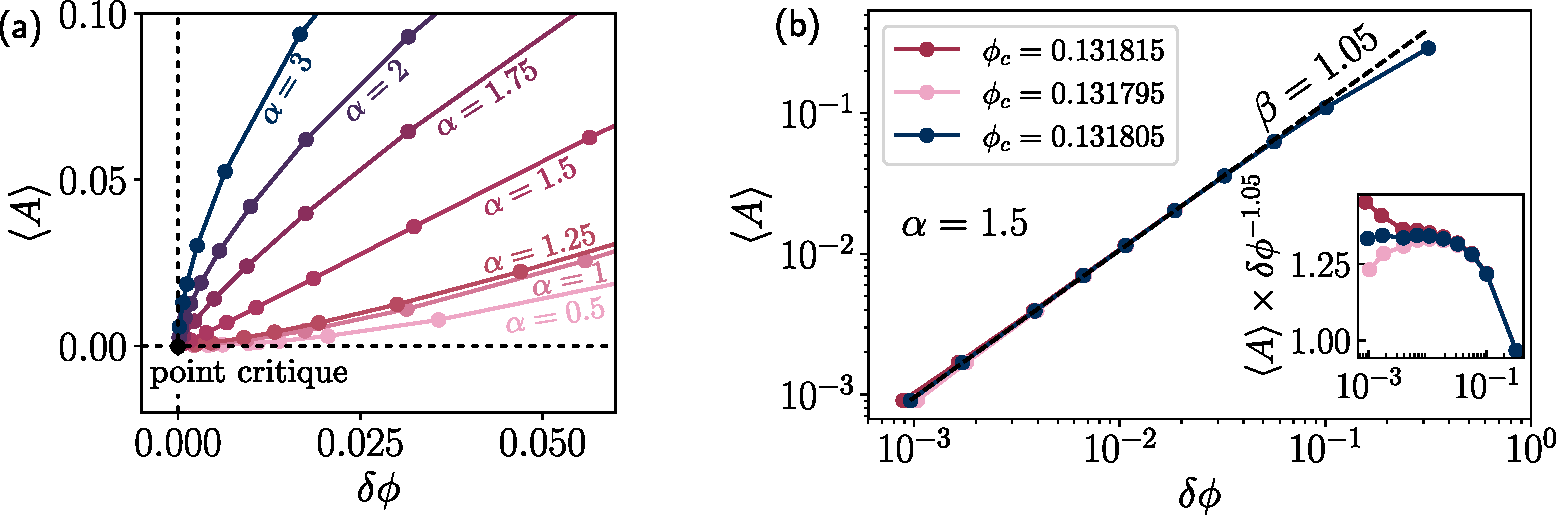
\includegraphics[width=\textwidth]{Chapitre3/Figures/BetaGamma/EvolMeanDeter.pdf}
	\caption{(a) Évolution de l'activité moyenne dans l'état stationnaire avec la distance au point critique pour différentes portée $\alpha$ des interactions médiées en 2D. (b) Exemple de détermination d'une densité critique $\phi_c$ dans le cas $\alpha = 1.5$ en 2D. Le choix $\phi_c = 0.131805$ est significativement meilleur que $\phi_c = 0.131815$ et $\phi_c = 0.131795$. En encart, la représentation compensée permet d'exacerber ces différences.}
	\label{fig:qualideter}
\end{figure}

\subparagraph{}Nous remarquons que cette évolution passe effectivement d'une forme concave à grand $\alpha$, à une forme convexe à petit $\alpha$. Ce comportement qualitatif est donc en accord avec les limites de courte portée ($\beta  \approx 0.64$ \cite{lubeck_universal_2004}) et de portée infinie ($\beta\approx 1.85$ \cite{mari_absorbing_2022}). Ainsi, comme dans le cas des sauts à longue portée, la criticalité semble évoluer continûment avec la portée de l'interaction.

\subparagraph{}Afin d'évaluer plus quantitativement cette évolution, il nous faut mesurer précisément l'exposant $\beta$ associé. Nous reprenons alors la méthode présentée à la \autoref{sec:methodchap2}. Un exemple de détermination dans le cas du $\alpha$-ROM pour $\alpha = 1.5$ est représenté à la \autoref{fig:qualideter}-(b). Ces déterminations sont alors bien plus compliquées que dans le cas des sauts à longue portée et ce pour deux raisons principales. La première est que le régime stationnaire est bien plus long à atteindre en présence de la diffusion des particules passives. Notamment, la décroissance initiale de l'activité et la transition entre régime transitoire et régime stationnaire associés sont bien moins abruptes. Ainsi, pour une courbe de convexité équivalente (i.e. $\beta$ équivalent), les simulations nécessitent plus de dix fois plus de pas de temps avant équilibration\footnote{De plus, les pas de temps du $\alpha$-ROM sont bien plus coûteux en termes de ressources numériques puisqu'ils font intervenir des calculs de FFT.}. La seconde vient du fait que les transitions convexes sont plus difficiles à caractériser. En effet, pour une distance au point critique équivalente, celles-ci impliquent des valeurs d'activités bien plus faibles (puisque $\langle A \rangle \sim \delta\phi^\beta$). Cela requiert alors des tailles de systèmes plus grandes et donc des simulations plus longues. Au final, l'équilibration de certains points aura nécessité plus de 800 heures de simulation continue sur des cartes graphiques de nouvelle génération\footnote{Les simulations présentées dans cet ouvrage ont été principalement réalisées sur des clusters de calcul GPU permettant un accès à des cartes graphiques NVIDIA V100 et A100}. En général, la caractérisation des transitions convexes amènera donc plus d'incertitudes.

\subsection{Évolution des exposants critiques}

\subsubsection{Exposants statiques}

\label{sec:TBLRRStat}

\subparagraph{}Les densités critiques déterminées permettent de représenter les courbes $\langle A \rangle = f(\delta\phi)$ en échelle logarithmique pour chaque $\alpha$ sur la \autoref{fig:evolmeanvar}-(a). Les exposants $\beta$ estimés par cette méthode sont reportés dans le \autoref{tab:expocrit_alphaROM} et leur évolution est résumée sur la \autoref{fig:expcritTBLRR}-(a).

\begin{figure}[h]
	\centering
	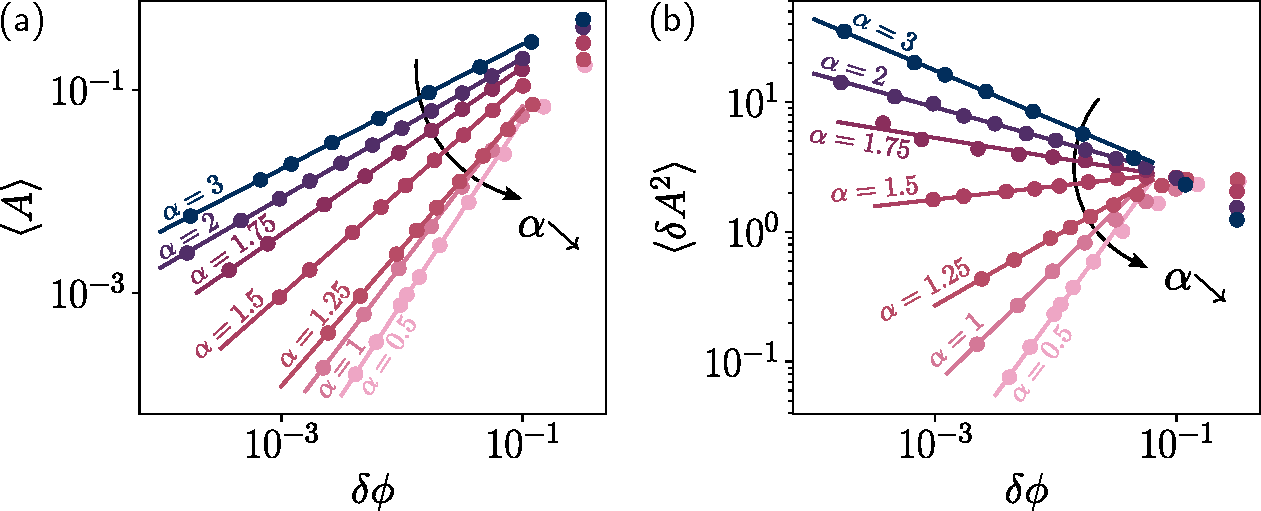
\includegraphics[width=0.9\textwidth]{Chapitre3/Figures/BetaGamma/EvolMeanVar_edited.pdf}
	\caption{(a) Évolution de la valeur moyenne de l'activité dans l'état stationnaire $\langle A \rangle$ en fonction de la distance au point critique $\delta\phi$ à différentes portées dans le $\alpha$-ROM en 2D. (b) Idem pour la variance $\langle \delta A^2 \rangle$}
	\label{fig:evolmeanvar}
\end{figure}

\subparagraph{}Pour déterminer l'exposant $\gamma^\prime$, comme dans le \autoref{chapter:TransportLP}, nous mesurons $\langle \delta A^2\rangle$ dans l'état stationnaire. La détermination de $\phi_c$ étant déjà effectuée, l'exposant se mesure par un simple ajustement de la courbe en échelle logarithmique. L'évolution des fluctuations en fonction de la portée est alors représentée sur la \autoref{fig:evolmeanvar}-(b). Nous observons un passage de fluctuations divergentes à l'approche du point critique pour les courtes portées à des fluctuations qui s'annulent pour les longues portées. Cette observation est à nouveau en accord avec les comportements limites de courte portée (CDP) et de portée infinie ($0$-ROM). Les valeurs des exposants $\gamma^\prime$ sont reportées dans le \autoref{tab:expocrit_alphaROM} et leur évolution est résumée sur la \autoref{fig:expcritTBLRR}-(a).

\begin{table}[h]
\centering
\begin{subtable}[t]{0.4\textwidth}
\begin{tabular}{ccccc}
\hline \hline $\alpha$ & $\beta$ & $\gamma^\prime$ & $\delta$ & $\nu_\perp^*$ \\
\hline \text{CDP} \cite{lubeck_universal_2004} & 0.64 & 0.37 & 0.42 & 0.80 \\
3 & 0.62 & 0.39 & 0.41 & 0.82 \\
2 & 0.69 & 0.26 & 0.42 & 0.82 \\
1.75 & 0.82 & 0.15 & 0.45 & 0.90 \\
1.5 & 1.05 & -0.10 & 0.49 & 1.00 \\
1.25 & 1.37 & -0.54 & 0.54 & 1.10 \\
1 & 1.56 & -0.90 & 0.62 & 1.11 \\
0.5 & 1.82 & -1.28 & 0.67 & 1.18 \\
0 \cite{mari_absorbing_2022} & 1.85 & -1.2 & - & 1.3 \\
\hline \hline
\end{tabular}
\caption{}
\end{subtable}
\hspace{0.1\textwidth}
\begin{subtable}[t]{0.4\textwidth}
\begin{tabular}{ccccc}
\hline \hline $\alpha$ & $\beta$ & $\gamma^\prime$ & $\delta$ & $\nu_\perp^*$ \\
\hline \text{CDP} \cite{lubeck_universal_2004} & 0.84 & 0.15 & 0.75 & 0.59 \\
3.5 & 0.84 & 0.16 & 0.74 & 0.61 \\
3 & 0.85 & 0.11 & 0.74 & 0.60 \\
2.5 & 0.95 & -0.03 & 0.74 & 0.62 \\
2 & 1.30 & -0.44 & 0.76 & 0.72 \\
1.75 & 1.49 & -0.82 & 0.75 & 0.72 \\
\hline \hline
\end{tabular}
\caption{}
\end{subtable}
\caption{Exposants critiques déterminés dans les modèles $\alpha$-ROM en 2D (a) et en 3D (b)}
\label{tab:expocrit_alphaROM}
\end{table}

\begin{figure}[h]
	\centering	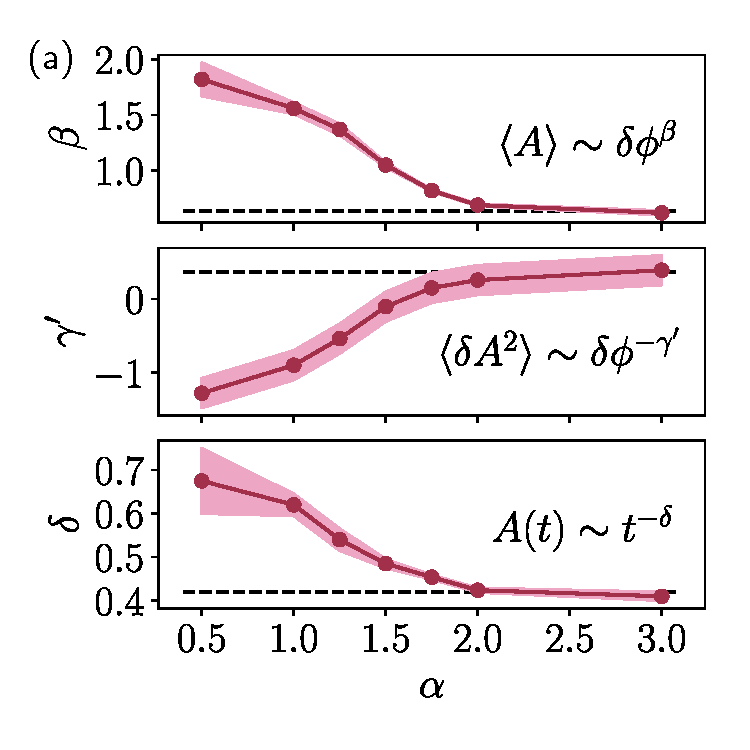
\includegraphics[width=0.48\textwidth]{Chapitre3/Figures/BetaGamma/exp_suspensions.pdf}
	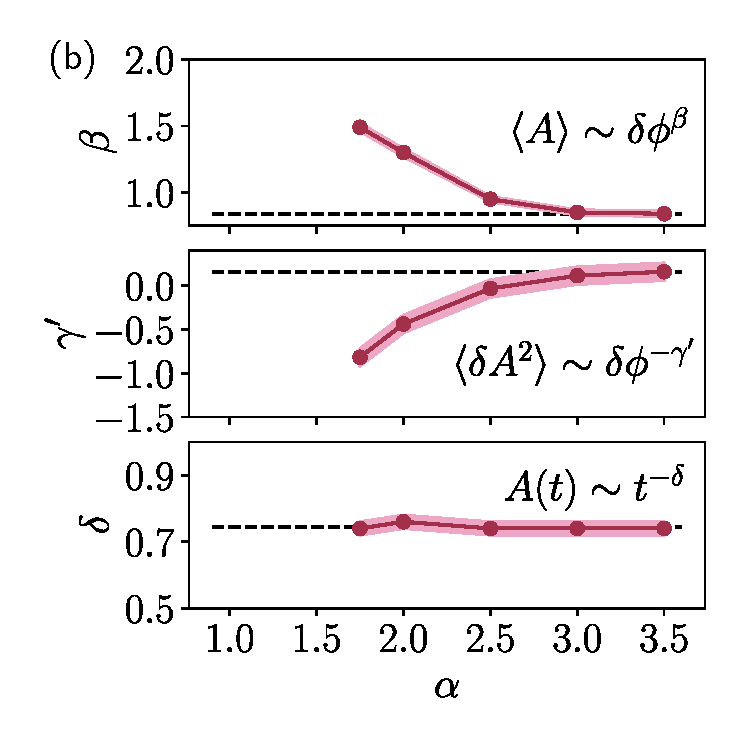
\includegraphics[width=0.48\textwidth]{Chapitre3/Figures/BetaGamma/exp_suspensions3D.pdf}
	\caption{Évolution des exposants critiques $\beta$, $\gamma^\prime$ et $\delta$  avec la portée dans le modèle $\alpha$-ROM en 2D (tableau de gauche) et en 3D (tableau de droite). Les zones colorées rose représentent les incertitudes de détermination.}
	\label{fig:expcritTBLRR}
\end{figure}

\paragraph{Zones d'évolution}

\subparagraph{}\`A la lumière de la \autoref{fig:expcritTBLRR}-(a), nous observons effectivement une évolution continue des deux exposants avec la portée. Notamment, l'évolution est significative entre $\alpha\approx 2$ et $\alpha \approx 1-0.5$, au-delà de quoi elle semble arriver à saturation des deux côtés\footnote{Pour $\alpha = 0.5$ la saturation se remarque par comparaison avec les valeurs obtenues pour $\alpha = 0$ \cite{mari_absorbing_2022}}. Par ailleurs les valeurs des exposants aux plus grands $\alpha$ rejoignent celles de la classe CDP : pour $\alpha=3$, l'accord est exact aux incertitudes de détermination près et pour $\alpha=2$ la différence est minime. Cela suggère donc de considérer $\alpha\approx 2$ comme limite de courte portée de la transition. \`A l'opposé du spectre, les exposants déterminés pour $\alpha = 0.5$ rejoignent aussi ceux déterminés dans le cas du $0$-ROM. Cette observation suggère alors $\alpha\approx 0.5$ comme la limite champ moyen de la transition. 

\paragraph{Comportement exotique et point singulier}

\subparagraph{}La spécificité de la limite de portée infinie rend cette variation du comportement critique avec la portée physiquement significative. En effet, si la courbe décrivant l'évolution du paramètre d'ordre reste concave ($\beta < 1$) pour $\alpha \gtrsim 1.5$, celle-ci change de convexité ($\beta >1$) pour $\alpha \lesssim 1.5$. C'est aussi autour de ce même point $\alpha \approx 1.5$ que le comportement des fluctuations critiques s'inverse, passant de divergent à évanescent. Le comportement exotique du 0-ROM est donc retrouvé dans toute la gamme d'évolution $\alpha \lesssim 1.5$. Il est donc envisageable de l'observer dans des systèmes systèmes réels présentant des interactions hydrodynamiques spatialisées.

\subparagraph{}Dans le cas du 0-ROM, cette double spécificité $\beta>1$, $\gamma^\prime<0$ peut être rationalisée dans le cadre de la relation d'hyperscaling \cite{lubeck_universal_2004} \cite{mari_absorbing_2022} :

\begin{equation}
	2\beta + \gamma^\prime = \nu_\perp D
\end{equation}

\noindent qui se retrouve vérifiée. Celle-ci permet en effet d'expliquer qu'une transition avec une valeur de $\beta$ anormalement grande donne lieu à une valeur de $\gamma^\prime$ anormalement petite. Étant donné que cette relation est aussi vérifiée dans la limite de courte portée CDP, nous pouvons supposer qu'elle l'est en fait dans toute la zone d'évolution présentée par le $\alpha$-ROM. Ainsi, l'annulation des fluctuations critiques s'expliquerait par la convexité de la transition à toute portée $\alpha \lesssim 1.5$.

\subparagraph{}Par ailleurs, si nous allons au bout de notre hypothèse, la relation d'hyperscaling permet de dériver pour chaque $\alpha$ un exposant de corrélation spatiale $\nu_\perp^*$\footnote{Nous utilisons la notation * pour signifier que cette valeur est dérivée d'une relation d'échelle et non dérivée.}. Dans le \autoref{tab:expocrit_alphaROM}-(a), nous répertorions le résultat de cette dérivation. Cet exposant hypothétique $\nu_\perp^*$ semble alors suivre une évolution continue avec la portée $\alpha$ qui lie les deux limites de CDP et du 0-ROM.

\subparagraph{}Le point $\alpha\approx 1.50$ se positionne donc à un changement drastique des propriétés de la transition. Remarquablement, ce point spécifique est décrit les exposants critiques $\beta$ et $\gamma^\prime$ associés champ moyen de CDP. Une différence majeure est alors que, dans le cas des interactions actives-passives, au contraire du cas des sauts à longue portée étudié au \autoref{chapter:TransportLP}, ce comportement n'est pas une limite mais il est effectivement dépassé pour des portées plus grandes.

\paragraph{Une limite non triviale}

\subparagraph{}En général, les champs moyens des théories critiques amènent à des valeurs triviales des exposants critiques ($\beta_\text{CDP}^\text{MF}=1$ par exemple). Or ici, la limite de portée infinie atteinte en $\alpha=0.5$, tout comme le 0-ROM caractérisé par Mari et al. \cite{mari_absorbing_2022}, est caractérisée par des exposants non-triviaux. Ces mesures peuvent alors suggérer que cette limite n'est en fait pas un équivalent champ moyen du système. 

\subparagraph{}Cette observation n'est pas si surprenante car certains éléments de la dynamique restent non-triviaux à portée infinie. En effet, même lorsque les interactions actives-passives sont à longue portée, les particules actives effectuent des sauts de taille finie et dans un espace de dimension finie. De plus, les particules passives, elles aussi diffusent dans un espace de dimension finie. La dimension de l'espace étant inférieure à la dimension critique supérieure de CDP $D_c = 4$, il est probable que ces mécanismes éloignent le modèle du champ moyen, même si les interactions médiées sont sous leur forme extrémale. Nous pouvons cependant nous attendre à approcher ce champ moyen en augmentant la dimension du système\footnote{Nous reviendrons sur cette idée à la \autoref{sec:interpret}}.

\subsubsection{Exposant dynamique}

\label{sec:TBLRRdyn}

\subparagraph{}Une autre possibilité pour caractériser la criticalité et son évolution avec la portée est d'étudier la transition d'un point de vue dynamique. Comme dans le cas du transport à longue portée, proche du point critique, le système relaxe vers l'état stationnaire de manière algébrique :

\begin{equation}
	 \langle A \rangle (t) \sim t^{-\delta}
\end{equation}

\noindent $\delta$ définissant un exposant critique universel. Il peut être alors intéressant de comprendre comment celui-ci varie avec $\alpha$ dans le cas du $\alpha$-ROM, et comment cette évolution se compare à l'évolution des exposants $\beta$ et $\gamma^\prime$.

\subparagraph{}Pour aborder cette question, nous reprenons la méthode de redimensionnement utilisée à la \autoref{sec:expdynjump}. Pour chaque $\alpha$, nous déterminons alors l'exposant $\delta$ associé en se basant sur les mesures précédentes de $\beta$ et $\phi_c$. Un exemple de redimensionnement obtenu dans le cas du $\alpha$-ROM est représenté à la \autoref{fig:deltadeter} pour $\alpha = 1.5$. Les valeurs mesurées pour chaque portée sont reportées dans le \autoref{tab:expocrit_alphaROM} et leur évolution est représentée sur la \autoref{fig:expcritTBLRR}-(a).

\begin{figure}[h]
	\centering
	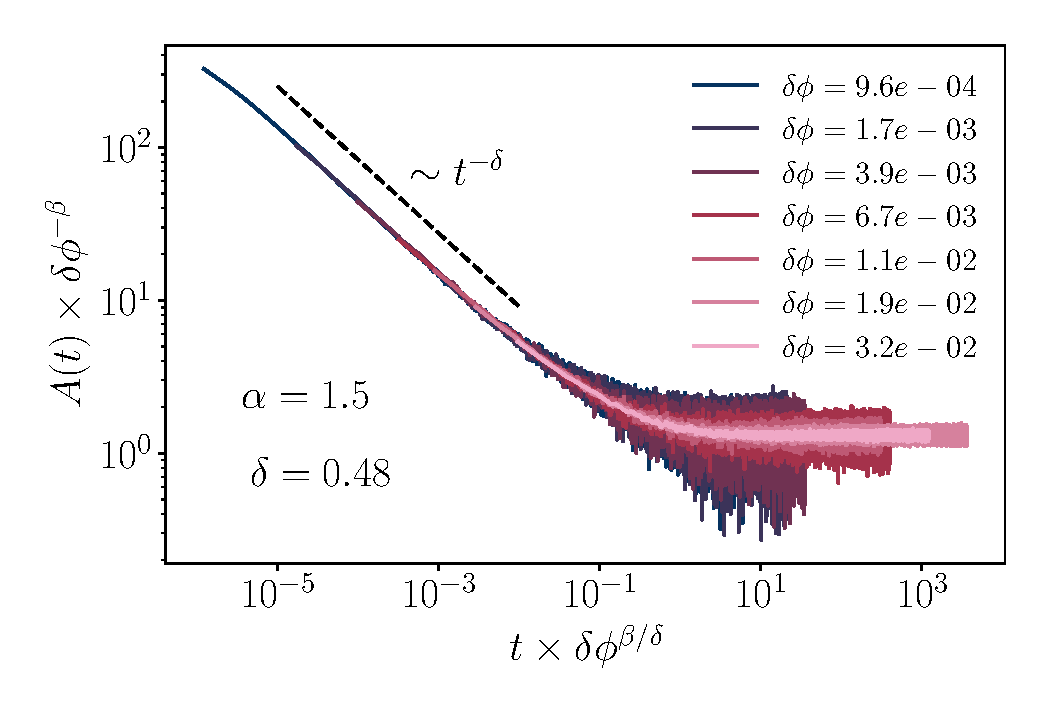
\includegraphics[width=0.6\textwidth]{Chapitre3/Figures/Delta/DeltaDetermination.pdf}
	\caption{Redimensionnement avec la distance au point critique $\delta\phi$ des évolutions de l'activité moyenne $\langle A \rangle$ avec le temps $t$ dans le cadre du $\alpha$-ROM en 2D pour $\alpha = 1.5$. \todo{moche, changer couleurs et mettre légende sur le pointillé}}
	\label{fig:deltadeter}
\end{figure}

\subparagraph{}Comme pour les exposants $\beta$ et $\gamma^\prime$, l'exposant dynamique $\delta$ évolue de sa valeur CDP pour $\alpha\gtrsim 2$ à une valeur de saturation pour $\alpha \lesssim 1-0.5$. Cela confirme donc la zone d'évolution continue précédemment déterminée.

\subparagraph{}Par ailleurs, dans la limite de longue portée $\alpha=0.5$, nous mesurons $\delta\approx0.67$. Cette valeur non-triviale conforte le fait que le système n'est pas dans sa limite champ moyen pour une portée infinie. Il est tout à fait envisageable que les sauts à courte portée des particules actives jouent un rôle dans la relaxation vers l'état stationnaire.

\subparagraph{}Enfin, si le point $\alpha\approx 1.5$ correspondait aux propriétés critiques statiques du champ moyen de CDP avec $\beta=1$ et $\gamma^\prime=0$, ses propriétés dynamiques semblent différer. En effet, pour $\alpha = 1.5$ nous mesurons $\delta\approx 0.49$, qui est notablement inférieur à $\delta_\text{CDP}^\text{MF}=1$. 

\subparagraph{}De manière générale, l'évolution des propriétés de relaxation du système semblent donc suivre une évolution très similaire à celle des propriétés statiques.

\subsubsection{Comparaison avec le cadre LR-CDP}

\subparagraph{}Dans cette partie, nous proposons de comparer les évolutions mesurées dans le $\alpha$-ROM en 2D avec celles prédites par le cadre LR-CDP, représentées par le LR-ROM au \autoref{chapter:TransportLP}. Pour rappel, dans le cadre LR-CDP représentant l'influence d'un transport de masse à longue portée, la criticalité du système évolue continûment dans la zone $3D/2 < \alpha < D+2$ soit $3 < \alpha < 4$ en 2D. Dans la limite de courte portée $\alpha > 4$, la criticalité retrouvée est celle de la classe CDP en 2D. Dans la limite de longue portée $\alpha < 3$, la criticalité retrouvée est celle de la classe CDP en champ moyen. 

\subparagraph{}D'un point de vue purement qualitatif, les évolutions mesurées dans le $\alpha$-ROM en 2D sont en accord avec cette image. En effet, dans ce cas, nous observons aussi une zone d'évolution continue des exposants séparant une limite de longue portée et une limite de courte portée. De plus, les évolutions des exposants avec $\alpha$ présentent la même tendance : $\beta$, $\gamma^\prime$, $\nu_\perp^*$ et $\delta$ augmentent avec $\alpha$.

\subparagraph{}Toutefois, du point de vue de la valeur des différents exposants, les transitions convexes $(\beta > 1)$ mesurées dans le $\alpha$-ROM pour $\alpha \lesssim 1.5$ se situent complètement en dehors du cadre LR-CDP, restreint à la description de transitions concaves. De plus, la zone continue d'évolution des exposants se situe à des portées bien plus grandes dans le cas du $\alpha$-ROM que dans le cadre LR-CDP. En effet, dans le cas du $\alpha$-ROM nous avons mesuré $0.5-1 \lesssim \alpha \lesssim 2$. La différence entre ce modèle numérique et le cadre LR-CDP ne prend donc pas uniquement place à grande portée mais à toute portée.

\subparagraph{}Finalement, les mesures des exposants critiques du $\alpha$-ROM montrent donc que le cadre LR-CDP ne permet pas de décrire l'influence des interactions hydrodynamiques sur le système malgré une évolution qualitative vaguement similaire¨.

\subsubsection{Extension à trois dimensions}

\subparagraph{}Afin de confirmer ces désaccords statiques et dynamiques, nous étendons notre analyse à des systèmes en trois dimensions. Nous rappelons que dans ce cas là, la théorie LR-CDP prédit une évolution continue des exposants dans la zone $4.5<\alpha<5$. Dans la limite de courte portée $\alpha>5$, les exposants prennent les valeurs reportées dans le \autoref{tab:expocrit_alphaROM}.

\subparagraph{}En appliquant la même méthode, nous étudions la criticalité des modèles pour $\alpha \in \{3.5, 3, 2.5, 2, 1.75\}$. Les analyses étant coûteuses numériquement et pour des raisons de temps, nous n'étudions pas le cas des très longues portées. Ce faisant, nous obtenons les évolutions de $\langle A \rangle$ et $\langle\delta A^2\rangle$ en fonction de $\delta\phi$ tracées à la \autoref{fig:evolmeanvar3D}. Les valeurs des exposants critiques sont alors reportées dans le \autoref{tab:expocrit_alphaROM} et leurs évolutions en fonction de la portée sont tracées sur la \autoref{fig:expcritTBLRR}-(b). Nous retrouvons alors à courte portée le comportement critique CDP en trois dimensions dès $\alpha \gtrsim 3$ et non $\alpha>5$. Pour des plus grandes portées $\alpha\lesssim 3$, l'évolution des exposants statiques $\beta$ et $\gamma^\prime$ est similaire au cas 2D, avec une augmentation progressive de $\beta$ conjointement à une diminution progressive de $\gamma^\prime$.

\begin{figure}[h]
	\centering
	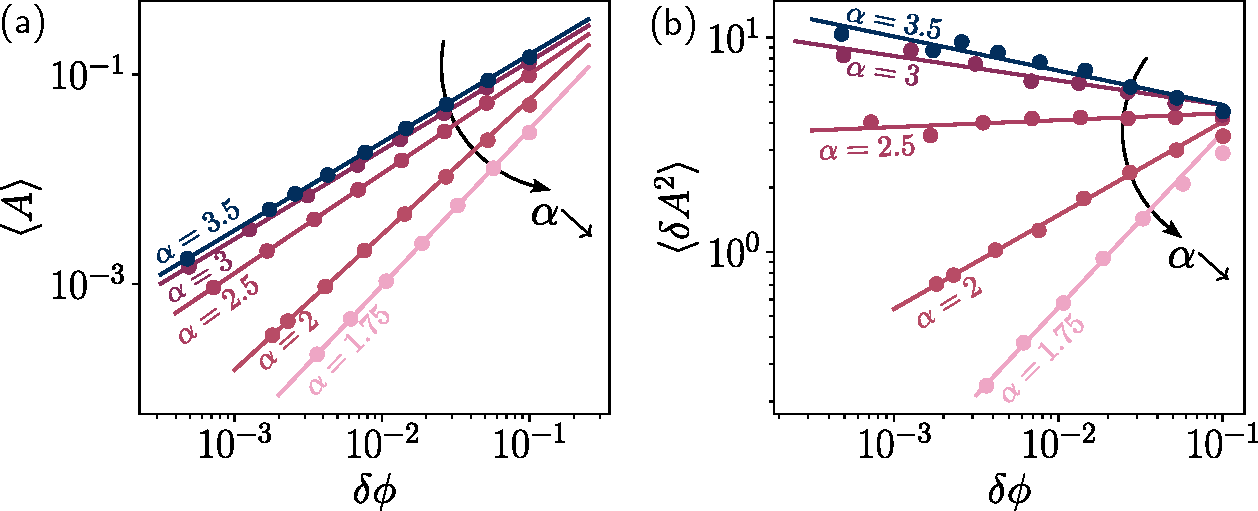
\includegraphics[width=0.9\textwidth]{Chapitre3/Figures/BetaGamma/EvolMeanVar3D_edited.pdf}
	\caption{(a) Évolution de la valeur moyenne de l'activité dans l'état stationnaire $\langle A \rangle$ en fonction de la distance au point critique $\delta\phi$ à différentes portées dans le $\alpha$-ROM en 3D. (b) Idem pour la variance $\langle \delta A^2 \rangle$}
	\label{fig:evolmeanvar3D}
\end{figure}

\subparagraph{}Par ailleurs, nous retrouvons aussi dans ce cas un point autour duquel la transition change simultanément de convexité et de comportement fluctuant, seulement cette fois localisé en $\alpha\approx 2.5$. En trois dimensions aussi, la criticalité des modèles $\alpha$-ROM est donc très différente de celle prévue par le cadre LR-CDP. Pour ce qui est du comportement dynamique, l'exposant $\delta$ opère cette fois une évolution quelque peu surprenante. En effet, celui-ci reste constant autour de $\delta \approx 0.74$, valeur associée à la classe CDP à courte portée. Dans cette dimension, les interactions médiées ne semblent donc pas affecter la relaxation vers l'état stationnaire.

\subparagraph{}Finalement, l'étude des modèles $\alpha$-ROM révèle un comportement critique très différent du cadre de référence LR-CDP en deux ou trois dimensions. Si l'on retrouve une zone d'exposants $\alpha$ pour lesquels la criticalité dépend continûment de la portée, celle-ci concerne des valeurs de $\alpha$ bien plus grandes que dans le cadre canonique. De plus, cette zone d'évolution continue n'est pas bornée par le champ moyen associé à celui de CDP, mais par une limite non-triviale en dimension finie, caractérisée par une convexité et des fluctuations évanescentes. Pourtant, l'évolution continue des exposants passe effectivement par un point caractérisé par les mêmes exposants statiques que le champ moyen CDP. Seulement, dans le cas des interactions médiées, celui-ci ne constitue pas un comportement limite. Les interactions médiées constituent donc un mécanisme permettant d'aller au-delà du champ moyen associé au comportement de courte portée, laissant place à un comportement exotique $\beta >1$, $\gamma^\prime<0$ sur toute une gamme de portées $\alpha$ physiquement envisageables.

\subsection{Hyperuniformité}

\label{sec:TBLRRHU}

\subparagraph{}Une autre manière de caractériser le modèle $\alpha$-ROM est de s'intéresser aux propriétés de structure de la transition. Dans le \autoref{chapter:introduction}, nous avons vu que proche du point critique, les modèles dans la classe CDP présentent un phénomène d'hyperuniformité. Dans le \autoref{chapter:TransportLP}, nous avons vu que dans le cadre LR-CDP, la propriété d'hyperuniformité est modifiée par la présence de transport à longue portée. Notamment, l'exposant $\alpha_\text{HU}$ caractérisant l'évolution du facteur de structure selon $S(\mathbf{q})\sim q^{\alpha_\text{HU}}$ évolue continûment de $\alpha_\text{HU}^\text{CDP, 2D}\approx 0.5$ à $\alpha_\text{HU}^\text{CDP, CM} = 0$ dans la zone $3<\alpha<4$ en 2D. L'hyperuniformité est donc perdue à longue portée dans ce cas. Les exposants critiques $\beta$, $\gamma^\prime$ et $\delta$ suivant une évolution différente du cadre LR-CDP dans le cas des interactions médiées à longue portée considérées dans le $\alpha$-ROM, il est naturel de se demander s'il en va de même pour l'exposant d'hyperuniformité. En d'autres termes, l'hyperuniformité est-elle aussi perdue dans la limite de longue portée des interactions hydrodynamiques ? 

\subparagraph{}En réalité, cette question a déjà été abordée par Mari et al. \cite{mari_absorbing_2022} lors de l'étude du 0-ROM. Dans ce cas de portée infinie, les auteurs ont montré que l'hyperuniformité est effectivement perdue à grande échelle. La question restante est alors de savoir comment s'opère ce changement de propriété avec l'évolution de la portée des interactions. Dans cette sous-section, nous nous basons sur des observations qualitatives pour fournir un début de réponse à cette question.

\subsubsection{Méthode}

\subparagraph{}Pour ce faire, nous utilisons, en plus de la méthode de box-counting présentée à la \autoref{sec:HUjumps}, une mesure du facteur de structure $S(\mathbf{q})$. Afin de rendre son calcul efficace, nous définissons un équivalent du champ de densité $\rho(\mathbf{r}_i)$ sur le réseau discret de pas $D_p$, utilisé pour calculer les interactions actives-passives. Dans chaque case située autour de $\mathbf{r}_i$, $\rho(\mathbf{r}_i)$ prend alors une valeur entière correspondant aux nombres de particules présentes dans cette case. Ce faisant, nous pouvons donc utiliser les algorithmes de FFT pour calculer $\hat{\rho}(\mathbf{q}_i)$ dans l'espace réciproque discret et on a alors directement\footnote{Est-ce qu'il faut mettre une moyenne en soi ?} :

\begin{equation}
	S(\mathbf{q}_i) = |\hat{\rho}(\mathbf{q}_i)|^2
\end{equation}

\noindent Pour évaluer l'évolution de $S(\mathbf{q})$ avec la norme du vecteur d'onde $q$ et donc sonder son évolution à petits $q$, nous réalisons une moyenne isotrope dans l'espace réciproque. En pratique, chaque point $S(q)$ est calculé par une moyenne sur l'anneau d'épaisseur $\frac{2\pi}{L}$ associé dans l'espace réciproque.

\subparagraph{}Afin de pouvoir comparer les répartitions de densité pour les différentes portées $\alpha$, nous nous plaçons à une distance fixée du point critique $\delta\phi \approx 1\times 10^{-2}$. Ce critère est en effet essentiel pour la comparaison puisque, comme nous l'avons vu au \autoref{chapter:TransportLP}, les propriétés d'hyperuniformité dépendent de la distance au point critique. Notamment, la propriété d'hyperuniformité est perdue à grande échelle pour des distances $\delta\phi$ trop grandes. Cette distance fixée est alors choisie de telle façon que les simulations associées à chaque portée puissent se dérouler sur des temps raisonnables ($<24~\text{h}$ pour une simulation individuelle). Afin d'obtenir une meilleure statistique, nous moyennons ces mesures sur plusieurs dizaines de configurations indépendantes dans l'état stationnaire. Les résultats obtenus sont alors représentés sur la \autoref{fig:HUTBLRR}-(a). En parallèle, les mesures de type box-counting sont effectuées et les résultats associés sont représentés sur la \autoref{fig:HUTBLRR}-(b).

\subsubsection{Résultats}

\begin{figure}[h]
	\centering
	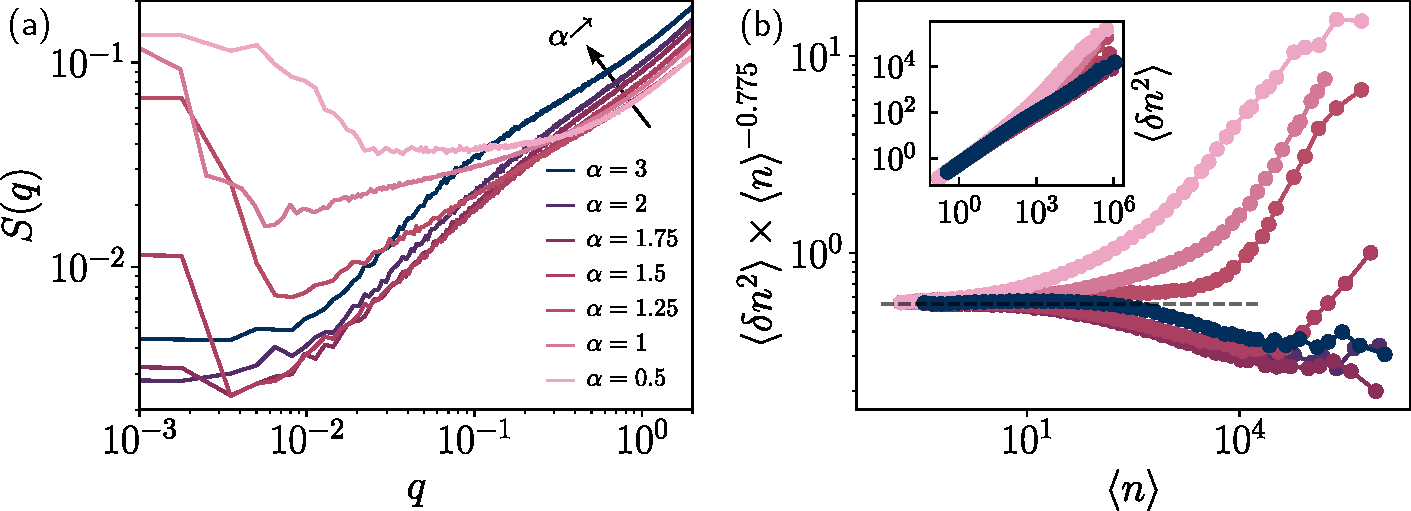
\includegraphics[width=\textwidth]{Chapitre3/Figures/HU/HUTBLRR.pdf}
	\caption{Hyperuniformité dans le modèle $\alpha$-ROM en 2D à $\delta\phi \approx 1\times 10^{-2}$. (a) Facteur de structure isotrope. (b) Méthode box-counting (voir \autoref{sec:HUjumps}) compensée par le comportement mesuré à courte portée $\alpha = 3$. En encart, les données brutes.}
	\label{fig:HUTBLRR}
\end{figure}

\subparagraph{}Dans la limite de longue portée $\alpha = 0.5$, nous retrouvons les résultats de Mari et al. \cite{mari_absorbing_2022} avec une perte du caractère évanescent de $S(\mathbf{q})$ à petits $q$. Dans la limite de courte portée $\alpha = 3$, l'allure globale de la courbe présente bien une diminution de $S(\mathbf{q})$ à petits $q$ bien que celle-ci ne semble pas suivre une loi de puissance évidente et sature à très petits $\mathbf{q}$. Cette saturation peut notamment s'expliquer par la distance finie au point critique examinée. L'observation de cette évanescence marque alors une forte différence avec le cas LR-CDP. En effet, dans ce cas, l'hyperuniformité est déjà complètement perdue à cette portée.  

\subparagraph{}Entre ces deux extrémités, les portées intermédiaires montrent une évolution intéressante. Si pour $\alpha > 1.5$ les facteurs de structure sont difficilement distinguables, pour $\alpha \leq 1.5$ leur évolution montrent d'abord décroissance plus faible à des valeurs de $q$ intermédiaires puis une augmentation à très petits $q$. Cette évolution suggère alors une perte de l'hyperuniformité à grande échelle dans le régime critique.

\subparagraph{}Un aspect de notre comparaison des différentes portées peut être questionné. Nous pouvons en fait imaginer deux façons de définir la distance à la transition, qui doit être fixée pour comparer les résultats obtenus pour différents $\alpha$. Ici, nous avons fait le choix de la caractériser via $\delta\phi$, qui est le choix le plus standard. Une autre possibilité aurait été de la caractériser via la valeur moyenne de l'activité dans l'état stationnaire $\langle A \rangle$. Dans ce cas, sachant que la convexité de la transition augmente avec la portée des interactions, nous en conclurions que les données présentées pour les plus petites valeurs de $\alpha$ sont bien plus proches de la transition que celles présentées pour les  plus grandes valeurs de $\alpha$. Pourtant, nous mesurons ici une perte du caractère hyperuniforme dans le cas des plus petites valeurs de $\alpha$. Sachant que l'on attend que les propriétés hyperuniformes se développent d'autant plus que le système est proche de la transtion, un changement de convention pour définir la distance à la transition ne permettrait donc pas de renverser la tendance observée ici, il l'exacerberait plutôt.

\subparagraph{}Cette tendance est moins évidente  mais se retrouve qualitativement dans le cas de la méthode de box-counting. En compensant l'évolution de $\langle \delta n^2 \rangle$ avec l'évolution mesurée à très courte portée $\langle \delta n^2 \rangle \sim \langle n \rangle^{0.775}$ sur la \autoref{fig:HUTBLRR}-(b), les évolutions pour $\alpha<1.5$ semblent aussi contraster avec celles de plus courtes portées $\alpha>1.5$, révélant un comportement localement "moins hyperuniforme" (i.e. un exposant effectif local $\alpha_\text{HU}^\text{eff}$ plus grand).

\subparagraph{}Finalement, cette analyse qualitative des propriétés d'hyperuniformité du $\alpha$-ROM semble montrer un changement autour de $\alpha = 1.5$. Pour $\alpha<1.5$, les observations suggèrent une hyperuniformité perdue à grande échelle. De la même manière que le transport d'activité à longue portée, les interactions médiées effacent donc le caractère hyperuniforme de la transition. Toutefois, la zone d'effet $\alpha < 1.5$ qualitativement identifiable ici est à nouveau très différente de celle prévue par le cadre de référence LR-CDP pour lequel on a $\alpha<3$. Une étude plus approfondie serait cependant nécessaire pour confirmer ces premières observations.

\subsection{Retour sur les cas physiques}

\subparagraph{}Au début de ce chapitre, nous avions identifié deux cas de portée pertinents dans le cadre de la transition de réversibilité des suspensions cisaillées cycliquement. Le premier, similaire au cas de l'expérience de Pine et. al \cite{pine_chaos_2005}, a lieu dans un milieu 3D peu confiné. Dans notre modélisation stroboscopique cela revient à $\alpha = 3$ dans le $\alpha$-ROM en 3D. Les résultats présentés au cours de cette section placent ce cas au cœur de la zone d'évolution continue des exposants avec $\beta > 1$ et $\gamma^\prime < 0$. La transition attendue est donc convexe.

\subparagraph{}Le second cas pertinent est le cas d'un cisaillement confiné entre deux plaques rigides, pour lequel on a $\alpha = 3$ dans un milieu quasi-2D. Notre étude du $\alpha$-ROM en 2D place alors cette situation dans la limite de courte portée, dans laquelle la transition adopte le comportement de la classe CDP, soit concave, avec des fluctuations qui divergent et des propriétés hyperuniformes. Ainsi, notre analyse indique que l'influence des interactions médiées à longue portée dépend fortement du système réel étudié, celles-ci n'ayant un impact sur le comportement critique que dans certains cas.

\subsection*{Conclusion de la section}

\subparagraph{}Finalement, l'analyse des propriétés statiques (\autoref{sec:TBLRRStat}), dynamiques (\autoref{sec:TBLRRdyn}) et de structure (\autoref{sec:TBLRRHU}) des transitions du $\alpha$-ROM montre que les interactions médiées dans ce système agissent sur le comportement critique d'une manière originale. Notamment l'évolution des exposant critiques avec l'exposant de portée $\alpha$ ne peut pas être comprise dans le cadre LR-CDP qui représente l'influence de sauts à longue portée dans le système. Plus particulièrement, nous observons une large gamme de portées en 2D et en 3D montrant un comportement convexe de la transition et évanescent des fluctuations. Ces observations n'étant pas rationalisables dans le cadre LR-CDP, il semble que la diffusion des particules passives dans le modèle constitue un mécanisme dont l'appréhension nécessite un nouveau cadre théorique.

\section{Interprétation}

\label{sec:interpret}

\subparagraph{}Que ce soit dans le cas du ROM appartenant à la classe CDP ou dans le cas du LR-ROM rattaché au cadre LR-CDP, la dynamique du système est contrôlée par le transport des particules actives. Comme nous l'avons détaillé dans la section précédente, ce mécanisme, par les cadres théoriques qu'il appelle, ne permet pas d'appréhender la criticalité dans les modèles $\alpha$-ROM.

\subparagraph{}Comme nous l'avons déjà évoqué au \autoref{chapter:introduction}, nous pensons que cette distinction est due à la nature des interactions à longue portée dans ces modèles. Celles-ci n'induisent en fait pas un transport des particules actives mais plutôt un bruit interne auquel sont soumises l'ensemble des particules du système. Au niveau de l'implémentation numérique de notre modèle, ce bruit interne est représenté par le processus diffusif composé de la succession des petits déplacements $\boldsymbol\delta^p$ (voir \autoref{fig:modelsusp}) induits par l'activité dans le système. Ce mécanisme propose alors un nouveau mode de création d'activité par rapport au ROM et au LR-ROM : deux particules passives peuvent devenir actives en se recouvrant après diffusion. Là où le processus de propagation de l'activité par transport (toujours présent dans le $\alpha$-ROM) est représenté par le processus de réaction-diffusion $A +B \xrightarrow[]{\lambda} 2A$ (voir \autoref{sec:CompCDP}), on pourrait formellement représenter ce nouveau mode de création de l'activité par l'équation :

\begin{equation}
	B +B \xrightarrow[]{} A + A
	\label{eq:meca_diff}
\end{equation}

\noindent les particules passives représentées par l'espèce $B$ ayant une dynamique stochastique dictée par l'espèce $A$. Nous pensons que c'est l'ajout de cette seconde réaction qui rend le comportement critique du $\alpha$-ROM très différent du cadre LR-CDP.

\subparagraph{}Dans ce chapitre, nous proposons un cadre d'interprétation de la transition de réversibilité dans les suspensions cisaillées cycliquement suivant ces lignes. Pour ce faire, nous partirons du modèle de Hébraud-Lequeux, incontournable dans le cas de la transition vers l'écoulement des fluides à seuil, pour développer un modèle champ moyen associé au $\alpha$-ROM. Se construisant via la notion de bruit interne, ce modèle permettra de mettre en évidence le mécanisme diffusif comme origine de la convexité des transitions précédemment caractérisées.

\subparagraph{}Nous généraliserons ensuite ce cadre champ moyen pour obtenir une première compréhension de  l'effet de la longue portée des interactions sur le processus diffusif et le comportement critique résultant. Cette analyse mènera à l'établissement d'un cadre théorique, alternative au cadre LR-CDP, qui nous permettra une première interprétation des résultats présentés dans la section précédente. 

\subparagraph{}Enfin, via des modifications de notre modèle numérique et des mesures complémentaires, nous mettrons en évidence les limites mais aussi les apports de cette approche de champ moyen pour interpréter les criticalité des modèles $\alpha$-ROM.

\subsection{Un cadre de description champ moyen}

\subparagraph{}Dans le cadre de la transition vers l'écoulement des fluides à seuil, la présence d'un bruit mécanique issu des interactions à longue portée médiées par le milieu a fait l'objet de diverses études \cite{lin_mean-field_2016, ferrero_criticality_2019}. D'un point de vue champ moyen, cette interprétation permet d'établir un modèle permettant d'expliquer la convexité de la transition observée expérimentalement. Ce modèle est le modèle de Hébraud-Lequeux\cite{hebraud_mode-coupling_1998}, que l'on présentera plus spécifiquement à la \autoref{sec:HL_def} du \autoref{chapter:yielding}. Du fait des similarités entre les transitions de réversibilité et d'écoulement présentées au \autoref{chapter:introduction}, notamment la présence d'un bruit interne, nous cherchons dans cette partie à définir un modèle équivalent au modèle Hébraud-Lequeux dans le cas de la transition de réversibilité afin d'expliquer les convexités mesurées dans la section précédente.

\subparagraph{}Pour ce faire, nous présenterons d'abord l'image champ moyen permettant d'établir un tel modèle. Nous montrerons alors que si celui-ci est très proche du modèle original de Hébraud-Lequeux, il existe entre ces deux formulations certaines différences. Malgré cela, nous montrerons par une résolution analytique que ce cadre d'interprétation champ moyen permet effectivement de décrire une transition convexe dans le cadre de la transition de réversibilité. Toujours inspiré du cadre de la transition vers l'écoulement, nous mettrons alors ce modèle à profit pour interpréter l'effet de la portée des interactions sur le comportement critique observé dans le $\alpha$-ROM.

\subsubsection{Première modélisation et diffusion normale}

\label{sec:diffnorm}

\paragraph{Présentation du modèle}

\subparagraph{}La philosophie du modèle de Hébraud-Lequeux capturant l'effet du bruit interne dans la transition vers l'écoulement consiste à se concentrer sur la dynamique effective d'un agent unique du système, diffusant vers une barrière sous l'action de l'activité globale. Nous proposons une image s'adaptant à cette formulation dans le cadre de la dynamique des particules dans le $\alpha$-ROM, illustrée à la \autoref{fig:LHLmodel}.

\subparagraph{}Considérons une particule passive dans notre modèle numérique. Au cours du temps, celle-ci diffuse jusqu'à rencontrer une autre particule. Dans une approche champ moyen négligeant toutes corrélations  (d'activité, de positions, ...), nous pouvons représenter les particules entourant notre particule d'intérêt par une cage effective de rayon $R$. En supposant une répartition des particules uniforme dans le système, la taille de cette cage peut être directement associée à la distance interparticulaire typique $l$ et donc à la densité de particules $\phi$. On a alors $R\sim \phi^{-1/D}$. En centrant cette zone de piégeage sur l'origine du repère, la particule cible positionnée en $\mathbf{r}$ peut donc prendre deux états : passive si elle n'entre pas en contact avec d'autres particules ($|\mathbf{r}|<R$), et active si elle sort de la cage effective ($|\mathbf{r}|>R$). 

\begin{figure}[h]
	\centering
	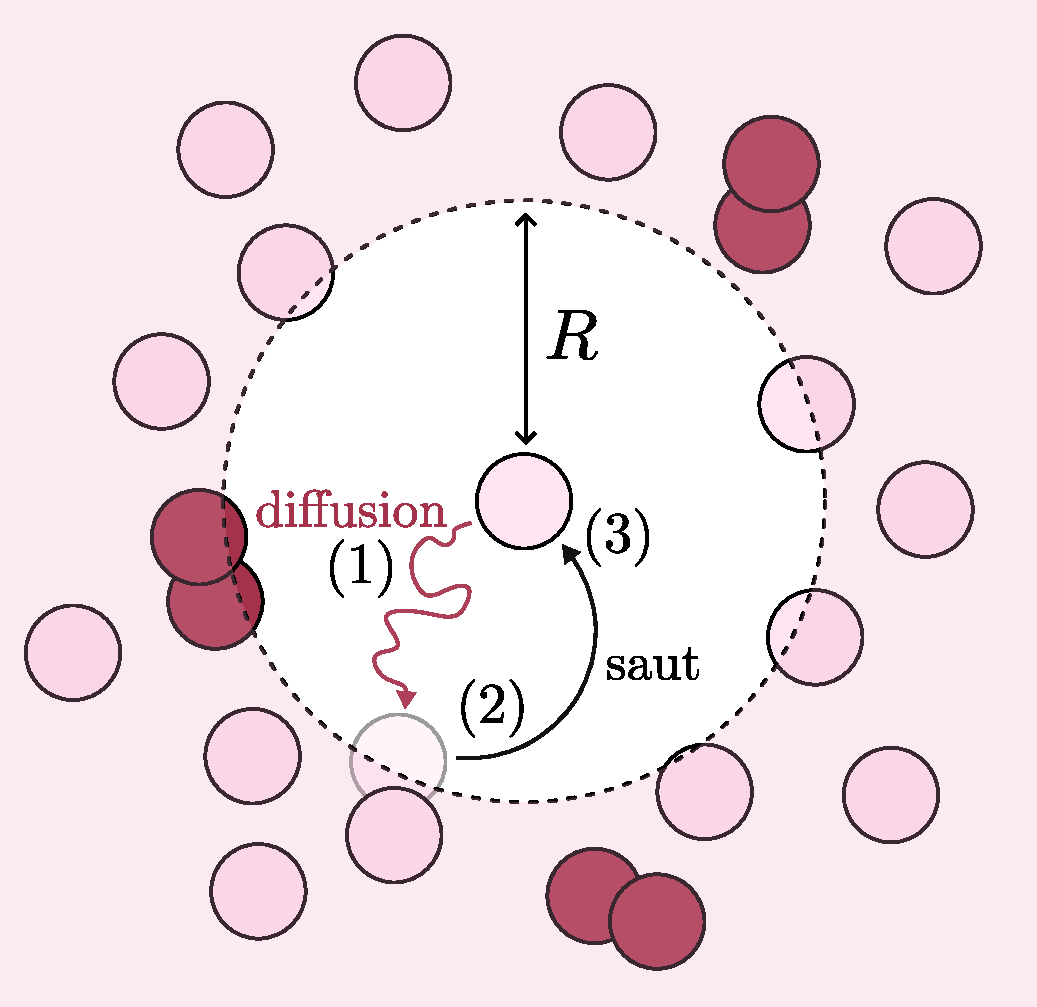
\includegraphics[width=0.5\textwidth]{Chapitre3/Figures/Interpretation/LHLModel.pdf}
	\caption{Représentation champ moyen de la dynamique du $\alpha$-ROM.}
	\label{fig:LHLmodel}
\end{figure}

\subparagraph{}Lorsque la particule est passive, celle-ci est soumise à un un bruit interne dont l'intensité est proportionnelle au nombre de particules actives dans l'environnement (i.e. l'activité dans le système). Dans cette vision statistique du problème où toutes les particules ont une dynamique équivalente, cette intensité du bruit est proportionnelle à la probabilité (notée $\Gamma\tau$ dans la suite) pour la particule d'être active. En première intention de modélisation, nous considérons ce bruit comme gaussien et donc que la particule diffuse avec un coefficient de diffusion $D=a\Gamma$ sous l'action de l'activité globale. 

\subparagraph{}Lorsque la particule est active, elle effectue un saut, comme dans le $\alpha$-ROM, sur un temps typique $\tau$. Dans notre modélisation champ moyen, nous considérons ce saut suffisamment grand pour replacer la particule à l'origine d'une nouvelle cage effective, la rendant de nouveau passive. 

\subparagraph{}Dans cette image simple, nous pouvons modéliser l'évolution de la distribution de probabilité $P(\mathbf{r})$ de la position $\mathbf{r}$ de la particule par les équations suivantes :

\begin{equation}
\begin{aligned}
    \partial_t P(\mathbf{r}, t) &= a\Gamma (t)\nabla^2 P(\mathbf{r}, t) - \frac{1}{\tau}\Theta(|\mathbf{r}|>R)P(\mathbf{r}, t) + \delta(\mathbf{r})\Gamma (t)\\ \Gamma (t) &= \frac{1}{\tau}\int_{|\mathbf{r}|>R}\mathrm{d}\mathbf{r}~P(\mathbf{r}, t)
    \label{eq:muHLDiff}
\end{aligned}
\end{equation} 

\noindent avec $a$ un paramètre réel. Le premier terme du membre de droite représente la diffusion de la particule ((1) sur la \autoref{fig:LHLmodel}), le second le processus de saut actif ((2) sur la \autoref{fig:LHLmodel}) et le troisième l'apparition dans une nouvelle cage ((3) sur la \autoref{fig:LHLmodel}). 

\subparagraph{}Comme nous le montrons juste après via sa résolution numérique, le modèle ainsi défini présente une transition de phase absorbante de paramètre d'ordre $\Gamma = \langle \Gamma (t) \rangle$ et de pramètre de contrôle $R$. Ces deux quantités sont les pendants directs de l'activité $\langle A \rangle$ et de la densité\footnote{Nous rappelons que dans notre modélisation champ moyen $R\sim \phi^{-1/D}$} $\phi$ dans le $\alpha$-ROM.


\paragraph{Comparaison avec la formulation originale}

\subparagraph{}Le modèle défini par cette image champ moyen dans le modèle de particules ressemble fortement au modèle de Hébraud-Lequeux utilisé dans le cadre de la transition vers l'écoulement (voir \autoref{sec:HL_def}). Dans ce cas où la variable d'intérêt est une contrainte locale $\sigma$ et non la position d'un objet, les équations prennent en fait la forme suivante :

\begin{equation}
\begin{aligned}
    \partial_t P(\sigma, t) &= -\dot{\gamma}\partial_\sigma P(\sigma, t)+a\Gamma (t)\nabla^2 P(\sigma, t) - \frac{1}{\tau}\Theta(|\sigma|>\sigma_Y)P(\sigma, t) + \delta(\sigma)\Gamma (t)\\
    \Gamma (t) &= \frac{1}{\tau}\int_{|\sigma|>\sigma_Y}\mathrm{d}\sigma~P(\sigma, t)
\end{aligned}
\label{eq:HL_comp}
\end{equation} 

\subparagraph{} On peut cependant remarquer deux différences principales entre ces deux formulations. La première est que la diffusion prend place dans un espace de dimension 1 dans le cadre de la transition vers l'écoulement alors qu'elle prend place dans un espace de dimension 2 ou 3 pour le modèle de suspensions. La seconde est la présence d'un terme additionnel dans l'\autoref{eq:HL_comp}, le premier du membre de droite. Ce terme en dérivée première de la distribution correspond à un forçage du système. Absent dans le cas du modèle de suspensions, il biaise la diffusion de la variable vers la barrière. Dans le cas de la transition de réversibilité, celui-ci reviendrait à l'ajout d'un mécanisme déterministe d'attraction vers le bord de la cage.

\subparagraph{}Cette seconde différence introduit une autre différence plus fondamentale. Dans le cas du modèle de Hébraud-Lequeux, le paramètre de contrôle habituel n'est pas $\sigma_Y$ (et donc de manière équivalente $R$ dans le cas des suspensions) mais plutôt la valeur moyenne de la variable d'intérêt $\Sigma = \int \mathrm{d}\sigma~P(\sigma,t)$. En effet, dans ce cas, via la brisure de symétrie opérée par le terme additionnel, celle-ci n'est plus nulle. La phénoménologie de la transition associée est donc décrite par la relation :

\begin{equation}
	\Gamma \sim (\Sigma - \Sigma_c)^\beta
	\label{eq:paramordre_HL}
\end{equation}

\subparagraph{}Dans le cadre du modèle d'écoulement, la résolution numérique de ce modèle donne $\beta=2$ et permet donc d'expliquer la convexité de la transition via le mécanisme de diffusion sous l'activité globale. On peut alors se demander si ce résultat tient toujours dans la formulation champ moyen adaptée au modèle de suspensions, malgré les deux différences mises en évidences dans cette partie.

\paragraph{Résolution en 2D}

\subparagraph{}Afin de montrer que ce modèle champ moyen permet effectivement de retrouver une transition convexe par ce mécanisme de diffusion, nous le résolvons en deux dimensions pour déterminer la relation $\Gamma \sim (R - R_c)^\beta$ à petits $\Gamma$. Pour ce faire, nous commençons par adimensionner l'\autoref{eq:muHLDiff} par les transformations :

\begin{equation}
	\tilde{t} = \frac{t}{\tau}, \quad \tilde{\mathbf{r}} = \frac{\mathbf{r}}{R}
\end{equation}

\noindent En nous plaçant de plus dans l'état stationnaire, nous obtenons alors :

\begin{equation}
    0 = \tilde{a}\tilde{\Gamma}\nabla^2 P(\tilde{\mathbf{r}}) - \Theta(|\tilde{\mathbf{r}}|>1)P(\tilde{\mathbf{r}}) + \delta(\tilde{\mathbf{r}})\tilde{\Gamma}, \quad \tilde{\Gamma} = \int_{|\tilde{\mathbf{r}}|>1}\mathrm{d}\tilde{\mathbf{r}}~P(\tilde{\mathbf{r}}),\quad \tilde{a} = \frac{a}{R^2}
\end{equation} 

\noindent Dans la suite de la résolution, nous omettrons les $\tilde{}$ pour alléger les notations. Sous cette transformation, le paramètre de contrôle est $a$, relié à la densité de particules via $a\sim \phi$ puisque nous rappelons que l'on a $R\sim 1/\sqrt{\phi}$.

\subparagraph{}Nous résolvons ensuite cette équation par morceaux dans les domaines disjoints $r<1$ (zone I) et $r>1$ (zone II). Dans la zone I, la résolution donne :

\begin{equation}
	P_\text{I}(\mathbf{r}) = c_1 \ln (r) + c_2, \quad (c_1, c_2) \in \mathbb{R}^2
\end{equation}

\noindent et dans la zone II :

\begin{equation}
	P_\text{II}(\mathbf{r}) = c_3 K_0\left( \frac{r}{\sqrt{a\Gamma}} \right), \quad c_3 \in \mathbb{R}
\end{equation}

\noindent avec $K_0$ la fonction de Bessel modifiée de seconde espèce d'ordre 0 \cite{abramowitz_handbook_1965}. La distribution $P(\mathbf{r})$ étant continue et de dérivée continue en $r=1$, on obtient finalement :

\begin{equation}
P(\mathbf{r}) = \left\{
    \begin{aligned}
    & c_3 \left( K_0\left( \frac{1}{\sqrt{a\Gamma}} \right) -K_1\left( \frac{1}{\sqrt{a\Gamma}} \right)\frac{\ln (r)}{\sqrt{a\Gamma}}\right), \quad r<1\\
    & c_3 K_0\left( \frac{r}{\sqrt{a\Gamma}} \right), \quad r>1
    \end{aligned}
    \right.
\end{equation}

\subparagraph{}La condition de normalisation de la distribution permet alors de déterminer la constante $c_3$. En effet on a :

\begin{equation}
	I_\text{I} = \int_0^1 \mathrm{d}r~ 2\pi r P(\mathbf{r}) = \pi c_3 K_0\left( \frac{1}{\sqrt{a\Gamma}} \right) + \frac{\pi c_3}{2\sqrt{a\Gamma}}K_1\left( \frac{1}{\sqrt{a\Gamma}} \right)
\end{equation}

\begin{equation}
	I_\text{II} = \int_0^\infty \mathrm{d}r~ 2\pi r P(\mathbf{r}) = 2\pi c_3 \sqrt{a\Gamma}K_1\left( \frac{1}{\sqrt{a\Gamma}} \right)
\end{equation}

\noindent en utilisant la propriété $(z^\nu K_\nu (z))^\prime = -z^\nu K_{\nu-1}(z)$. Nous obtenons alors :

\begin{equation}
\frac{1}{c_3} = \pi K_0\left( \frac{1}{\sqrt{a\Gamma}} \right) + \frac{\pi}{2\sqrt{a\Gamma}}K_1\left( \frac{1}{\sqrt{a\Gamma}} \right)+2\pi \sqrt{a\Gamma}K_1\left( \frac{1}{\sqrt{a\Gamma}} \right)
\end{equation}

\subparagraph{}La valeur de $\Gamma$ dans l'état stationnaire est alors donnée par la relation d'auto-cohérence :

\begin{equation}
	\Gamma = \frac{2\pi \sqrt{a\Gamma}K_1\left( \frac{1}{\sqrt{a\Gamma}} \right)}{\pi K_0\left( \frac{1}{\sqrt{a\Gamma}} \right) + \frac{\pi}{2\sqrt{a\Gamma}}K_1\left( \frac{1}{\sqrt{a\Gamma}} \right)+2\pi \sqrt{a\Gamma}K_1\left( \frac{1}{\sqrt{a\Gamma}} \right)}
	\label{eq:blabla}
\end{equation}

\noindent Étant intéressés par le comportement asymptotique à petits $\Gamma$, nous développons les fonctions de Bessel asymptotiquement selon :

\begin{equation}
	K_\nu (x) \sim \sqrt{\frac{\pi}{2x}}e^{-x}\left( 1+\frac{4\nu^2-1}{8x}+\mathcal{O}(1/x^2) \right)
\end{equation}

\noindent En développant le membre de droite de l'\autoref{eq:blabla} au premier ordre non-trivial nous obtenons finalement :

\begin{equation}
	\Gamma = 4a\Gamma\left( 1-2\sqrt{a\Gamma}+\mathcal{O}(a\Gamma) \right)
\end{equation}

\noindent Il y a alors deux cas possibles selon la valeur de $a$ et sa comparaison avec la valeur critique $a_c = \frac{1}{4}$. Pour $a<a_c$, la seule solution est $\Gamma = 0$. Pour $a>a_c$, une autre solution $\Gamma > 0$ apparaît, se comportant comme $\Gamma \sim (a-a_c)^2$. Si l'on revient aux variables avant adimension, cela revient à :

\begin{equation}
	\Gamma \sim (R-R_c)^2
	\label{eq:resolhl2d}
\end{equation}

\subparagraph{}Ainsi, ce modèle rend bien compte d'une transition de phase absorbante avec une phase absorbée $\Gamma = 0$ lorsque la cage effective est suffisamment grande $R>R_c$, et une phase active $\Gamma >0$ lorsque celle-ci est suffisamment petite $R<R_c$. Étant donné que l'on a $R\sim 1/\sqrt{\phi}$ dans l'image champ moyen et que $\Gamma$ correspond à l'activité dans le système, le comportement qualitatif de transition du $\alpha$-ROM est bien retrouvé. De plus, dans l'image champ moyen celui-ci est donc caractérisé par un exposant critique $\beta = 2$. Ce modèle simple permet donc effectivement de retrouver la convexité de la transition de réversibilité. Les différences entre le modèle champ moyen d'écoulement et celui de réversibilité n'impactent donc pas la criticalité du système.

\subparagraph{}Via ce nouveau cadre de modélisation statistique, nous sommes donc capables d'interpréter la convexité des transitions observées dans le $\alpha$-ROM. Toutefois, cette approche champ moyen ne permet pas de rendre compte de l'évolution de cette convexité avec la portée des interactions associées puisque celles-ci sont encodées dans un terme de bruit gaussien générique, quelque soit $\alpha$. Dans la partie suivante, nous montrons, en suivant les lignes d'études menées sur la transition vers l'écoulement, que l'effet de la portée des interactions peut en fait être introduit dans cette image simple afin de formuler des prédictions quant à l'évolution de l'exposant $\beta$ avec $\alpha$ dans un cadre champ moyen.
 
\subsubsection{Influence de la longue portée et diffusion anormale}

\label{sec:LPHL}

\subparagraph{}Dans le cadre de la transition vers l'écoulement, les auteurs de l'étude \cite{lin_mean-field_2016} ont montré que la modélisation gaussienne du bruit n'était pas toujours la plus pertinente pour décrire l'effet des interactions à longue portée dans le système. Dans cette partie, nous reprenons cet argument pour le transposer au modèle de suspensions.

\paragraph{Interactions à longue portée et distributions de bruit interne}

\subparagraph{}En fait, du fait de la propriété de décroissance algébrique du propagateur hydrodynamique $ \mathcal{G}$, le bruit interne peut être largement distribué. Dans l'image champ moyen développée précédemment, cela revient à considérer que la particule cible effectue des sauts de Lévy de taille $\Delta$ distribués selon :

\begin{equation}
	P(\Delta) \sim \frac{1}{\Delta^{1+\mu}}
\end{equation}

\noindent avec $\mu < 2$\footnote{Dans la limite $\mu \geq 2$, la variance de la distribution est finie et donc ce processus se ramène à une marche aléatoire gaussienne}. Dans notre modélisation probabiliste, cela revient donc à modifier l'\autoref{eq:muHLDiff} selon :

\begin{equation}
\begin{aligned}
    \partial_t P(\mathbf{r}, t) &= -a\Gamma (t)|\nabla|^{\mu} P(\mathbf{r}, t) - \frac{1}{\tau}\Theta(|\mathbf{r}|>R)P(\mathbf{r}, t) + \delta(\mathbf{r})\Gamma (t)\\
     \Gamma (t) &= \frac{1}{\tau}\int_{|\mathbf{r}|>R}\mathrm{d}\mathbf{r}~P(\mathbf{r}, t)
\end{aligned}
    \label{eq:muHL}
\end{equation}

\noindent avec $|\nabla|^{\mu}$ l'opérateur de dérivée fractionnaire déjà défini au \autoref{chapter:TransportLP} dans le cadre du transport à longue portée. Celui-ci traduit alors une diffusion anormale de la particule.

\subparagraph{}D'un point de vue champ moyen, nous pouvons déterminer la valeur de $\mu$ en fonction de la portées des interactions hydrodynamiques. Dans le cas où le bruit interne provient d'une unique particule active et où les interactions médiées décrites par le propagateur $\mathcal{G}(\mathbf{r})$ décroissent comme $1/r^\alpha$, la distribution associée est :

\begin{equation}
	P(\Delta) \sim \int \mathrm{d}\mathbf{r}~\delta\left( \mathcal{G}(\mathbf{r})-\Delta \right)\sim \frac{1}{\Delta^{1+D/\alpha}}
\end{equation}

\noindent et on a donc $\mu = D/\alpha$. Ce résultat basé sur un évènement unique reste valable lorsque l'on considère un ensemble de particules actives dans le système, mais à la condition que l'activité dans le système soit totalement décorrélée et n'est donc valable que dans la limite de champ moyen.

\subparagraph{}Nous nommons le modèle généralisé représenté par l'\autoref{eq:muHL}, le modèle $\mu$-Hébraud-Lequeux. Il est alors intéressant de voir comment cette généralisation permet de modifier l'exposant $\beta$ associé en fonction du paramètre $\mu$, afin d'interpréter la dépendance en $\alpha$ observée dans les simulations numériques.

\paragraph{Résultats dans le cadre de la transition vers l'écoulement}

\subparagraph{}La généralisation du modèle de Hébraud-Lequeux à un bruit largement distribué a déjà été étudié dans le cas de la transition vers l'écoulement. Via cette formulation, les auteurs des études \cite{lin_mean-field_2016, lin_microscopic_2018} sont parvenus à formuler des prédictions sur le comportement critique du modèle en fonction de l'exposant de bruit $\mu$. Dans cette partie, nous rappelons brièvement ces résultats. Ceux-ci sont en fait utiles à notre étude puisque l'on peut penser qu'ils se transposent à notre modèle $\mu$-Hébraud-Lequeux, de la même manière que dans le cas d'une diffusion normale.

\subparagraph{}Par une étude quasistatique de la généralisation de l'\autoref{eq:HL_comp}, il a été montré que l'exposant $\beta$ caractérisant la transition vers l'écoulement via l'\autoref{eq:paramordre_HL} évoluait en fonction de $\mu$ selon :

\begin{equation}
	\beta = \left\{
	\begin{aligned}
	&2, \quad \mu \geq 2\\
	&\mu, \quad 1<\mu\leq2\\
	&1, \quad \mu < 1
	\end{aligned}
	\right.
	\label{eq:PredicBetaLW}
\end{equation}

\noindent retrouvant $\beta = 2$ dans la limite gaussienne et $\beta = 1$ dans la limite $\mu<1$ où la dynamique est dominée par le terme de forçage \cite{lin_mean-field_2016}.

\subparagraph{}Par ailleurs, dans cette même limite d'activité nulle ($P(\sigma>\sigma_Y)=0$), il a été démontré que la distribution $P(\sigma)$ présentait un comportement algébrique proche de la barrière $\sigma = \sigma_Y$ \cite{lin_mean-field_2016} :

\begin{equation}
	P(\sigma_Y-\sigma) \sim (\sigma_Y-\sigma)^\theta
\end{equation}

\noindent avec $\theta$ l'exposant de pseudo-gap. Dans le cas où le système n'est pas forcé, se rapprochant alors du cas de notre modèle de suspensions, il a été montré que cet exposant dépend de l'exposant de bruit $\mu$ selon :

\begin{equation}
	\theta = \left\{
	\begin{aligned}
	&\frac{\mu}{2}, \quad \mu \leq 2\\
	&1, \quad \mu \geq 2
	\end{aligned}
	\right.
	\label{eq:PredicThetaLW}
\end{equation}

\subparagraph{}Le modèle d'écoulement étudié dans \cite{lin_mean-field_2016, lin_microscopic_2018} permet donc de qualifier une évolution de la criticalité de la transition vers l'écoulement en fonction du bruit interne associé. \'Etant très similaire au modèle $\mu$-Hébraud-Lequeux établi dans le cas de la transition de réversibilité, nous nous demandons si nous pouvons transposer ces résultats analytiques à notre cadre d'interprétation champ moyen. En d'autres termes, l'\autoref{eq:PredicBetaLW} et l'\autoref{eq:PredicThetaLW} sont-elles toujours valables dans ce cas ?

\subparagraph{}Dans le cadre de l'image champ moyen que nous avons proposé pour la transition de réversibilité, l'exposant $\beta$ définit la relation entre l'activité $\Gamma$ et la taille de la cage effective $R$ selon :

\begin{equation}
	\Gamma \sim (R-R_c)^\beta
\end{equation}

\noindent Pour ce qui est de l'exposant de pseudo-gap, par transposition, celui-ci définit la relation :

\begin{equation}
	P(R-|\mathbf{r}|)\sim (R-|\mathbf{r}|)^\theta
\end{equation}

\subparagraph{}Les raisons pour lesquelles cette correspondance de valeur des exposants pourrait ne pas fonctionner sont les différences entre les modèles présentées à la \autoref{sec:diffnorm}, à savoir la différence de dimension et l'existence ou non d'un terme de forçage qui implique un changement du paramètre de contrôle. Toutefois, la correspondance entre les deux modèles dans le cas de la diffusion normale (où l'on trouve $\beta = 2$ dans les deux cas) suggère que ces différences n'impactent pas réellement le comportement critique de la transition. Pour s'en assurer, nous proposons une résolution numérique du modèle $\mu$-Hébraud-Lequeux dans la partie suivante.

\paragraph{Résolution numérique}

\subparagraph{}Afin de confirmer que le modèle $\mu$-Hébraud-Lequeux suit bien le même comportement critique que dans le cas des études \cite{lin_mean-field_2016, lin_microscopic_2018}, nous résolvons l'\autoref{eq:muHL} par une méthode numérique. Celle-ci, détaillée dans la \autoref{sec:ResolNumMuHL}, consiste à interpréter cette équation comme une équation de Fokker-Planck et de la résoudre statistiquement par son équivalent en équation de Langevin. Il est alors possible de déterminer l'évolution de $\Gamma$ avec $R$ et d'en déduire l'exposant critique $\beta$ associé. La méthode de détermination de l'exposant $\beta$ suit alors le même principe que celle dans le cas du $\alpha$-ROM. Les résultats obtenus en 1D et en 2D sont reportés sur la \autoref{fig:LHLNum} où nous avons aussi représenté le comportement prédit dans la théorie homologue pour la transition vers l'écoulement.

\begin{figure}[h]
	\centering
	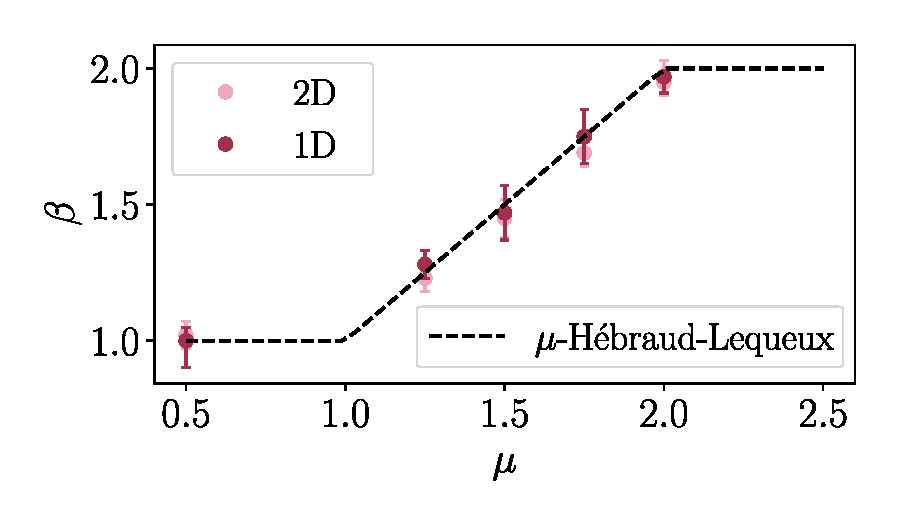
\includegraphics[width=0.6\textwidth]{Chapitre3/Figures/Interpretation/beta_alpha_LevyHL2D.pdf}
	\caption{Évolution de l'exposant $\beta$ mesuré par la résolution numérique de l'\autoref{eq:muHL} en 1D et en 2D (voir \autoref{sec:ResolNumMuHL}). En pointillés noirs, le comportement du modèle de Lin et al. \cite{lin_microscopic_2018}}
	\label{fig:LHLNum}
\end{figure}

\subparagraph{}La détermination des exposants n'est pas aisée car elle est coûteuse numériquement, laissant ainsi place à de larges incertitudes de mesure. Toutefois, que ce soit en une ou deux dimensions, les points mesurés montrent un plutôt bon accord avec l'attendu théorique. Les points en 1D semblent ainsi montrer que l'ajout du terme de forçage ne modifie pas la criticalité de la transition, tandis que les points en 2D suggèrent que cette théorie s'étend trivialement aux dimensions supérieures.

\subparagraph{}Pour la suite de notre analyse nous considérerons donc que le modèle $\mu$-Hébraud-Lequeux suit effectivement une criticalité dictée par l'\autoref{eq:PredicThetaLW} et l'\autoref{eq:PredicBetaLW}. En d'autres termes, dans une gamme d'exposants $1<\mu<2$, la criticalité du modèle dépend continûment de $\mu$ avec $\beta = 2\theta = \mu$. Pour $\mu < 1$, le modèle atteint une limite dans laquelle on a trivialement $\beta = 1$ et $\theta = \mu/2$. Pour $\mu>2$, le modèle atteint une limite diffusive dans laquelle nous avons montré que $\beta = 2$, et $\theta = 1$.

\subparagraph{}Le raisonnement présenté à la \autoref{sec:LPHL} implique que $\mu$ est inversement proportionnel à la porté des interactions $\alpha$. Dans le cadre champ moyen représenté par le modèle $\mu$-Hébraud-Lequeux, la portée des interactions semble donc affecter le comportement critique de la même manière que nous l'avons observé dans le $\alpha$-ROM : la convexité de la transition augmente avec la portée. Afin de tester plus spécifiquement cette image champ moyen et sa pertinence pour décrire le mécanisme à l'oeuvre dans les simulations numériques en dimension finie, nous proposons dans la partie suivante un test plus spécifique des prédictions du modèle.


\subsection{Interprétation champ moyen du mécanisme de diffusion dans le $\alpha$-ROM}

\subparagraph{}L'image développée précédemment via le modèle $\mu$-Hébraud-Lequeux est une image champ moyen du mécanisme de diffusion des particules passives et de son influence sur la criticalité de la transition. Puisque champ moyen, elle repose sur deux approximations essentielles : celle que la dynamique des particules actives est décorrélée et celle que la dynamique des particules passives l'est aussi. Dans ce cas, il est possible de faire un lien entre les différents exposants caractérisant le problème.

\subparagraph{}Le premier lien réside dans la relation reliant la portée des interactions caractérisée par l'exposant $\alpha$ et la distribution du bruit interne caractérisée par l'exposant $\mu$. Dans le cas d'une dynamique des particules actives décorrélée, nous avons en effet $\mu = D/\alpha$ comme nous l'avons montré à la \autoref{sec:LPHL}. Le second lien réside dans l'influence de cet exposant $\mu$ sur la criticalité du modèle caractérisée par les exposants $\beta$ et $\theta$. Celui-ci est représenté par l'\autoref{eq:PredicThetaLW} et l'\autoref{eq:PredicBetaLW}. Notamment, pour $1<\mu<2$, nous avons $\beta = \mu$ et $2\theta = \mu$ et donc $\beta = 2\theta$. 

\subparagraph{}Dans cette partie, nous cherchons à tester la pertinence de cette image champ moyen pour interpréter les transitions observées dans le $\alpha$-ROM. La difficulté est que le $\alpha$-ROM est un modèle numérique complexe. Pour deux raisons principales, nous nous attendons d'emblée à ce que celui-ci se démarque de l'image champ moyen. La première raison est que celui-ci fait intervenir deux mécanismes différents pour la création d'activité, comme nous l'avons mentionné au début de cette section. Le premier mécanisme est celui de la diffusion des particules passives et le second est celui du transport des particules actives. Dans sa construction, le modèle $\mu$-Hébraud-Lequeux basé uniquement sur ce premier mécanisme ne prétend donc pas représenter la criticalité complète du $\alpha$-ROM mais seulement un aspect de celle-ci. La seconde raison est que le $\alpha$-ROM présente une dynamique des particules passives et actives en dimension finie, et donc a priori non exempte de corrélation. 

\subparagraph{}Afin de déterminer si le modèle $\mu$-Hébraud-Lequeux est un cadre d'interprétation pertinent, nous ne pouvons donc pas nous réduire à une comparaison de ses prédictions avec les résultats directement obtenus dans le cadre du $\alpha$-ROM. \`A la place, nous proposons d'étudier la validité de ces prédictions dans des limites du modèle $\alpha$-ROM où les points de divergence conceptuels s'estompent. Si dans la limite où les hypothèses de l'image champ moyen sont satisfaites nous retrouvons les prédictions associées au modèle $\mu$-Hébraud-Lequeux, cela constitue une preuve que celui-ci permet bien de représenter le mécanisme de diffusion du $\alpha$-ROM dans son aspect champ moyen.

\subsubsection{Image champ moyen dans une dynamique d'activité décorrélée}

\paragraph{Approche du champ moyen par les grandes dimensions}

\subparagraph{}Afin de pouvoir tester la validité de l'image proposée par le modèle $\mu$-Hébraud-Lequeux, nous proposons donc d'isoler le mécanisme de création de l'activité par diffusion des particules passives dans le $\alpha$-ROM et de le considérer dans sa version champ moyen. 

\subparagraph{}Pour ce faire, nous modifions d'abord le modèle en changeant la dynamique des particules actives. Au lieu de faire des sauts finis, nous considérons cette fois que celles-ci sont redistribuées aléatoirement dans l'espace. Cela équivaut donc à faire des sauts de taille infinie. De ce fait, en accord avec les résultats du \autoref{chapter:TransportLP}, la dynamique d'activité devient champ moyen. Cela permet deux choses : isoler l'influence du mécanisme de diffusion puisque c'est dans ce cas là le seul capable de produire une criticalité non-triviale, et supprimer les corrélations dans la dynamique d'activité qui pourraient modifier la relation simple $\mu = D/\alpha$.

\subparagraph{}Pour rendre champ moyen le mécanisme de diffusion des particules passives, nous proposons de supprimer les corrélations dans leur dynamique en considérant des dimensions élevées du système. Dans cette limite, nous nous attendons à ce que cette version modifiée du $\alpha$-ROM représente le cadre de modélisation du modèle $\mu$-Hébraud-Lequeux. Nous proposons alors, pour tester l'image champ moyen, de mesurer l'exposant $\beta$ dans ce modèle numérique pour la valeur de portée des interactions $\alpha = 0$ et pour les dimensions $D\in\{2,3,4,6\}$. Si le cadre $\mu$-Hébraud-Lequeux est effectivement le bon champ moyen associé, nous nous attendons à mesurer $\beta = 2$ dans la limite de grande dimension.

\subparagraph{}Pour ce faire, nous reprenons les méthodes utilisées précédemment dans le cadre du $\alpha$-ROM. Nous répertorions alors sur la \autoref{fig:Ddep} des mesures préliminaires de l'exposant $\beta$ pour ces différentes dimensions. Il est à noter que plus la dimension du système est grande, plus le coût numérique des simulation l'est aussi, rendant difficilement accessible une estimation très précise de l'exposant. Des résultats préliminaires nous permettent toutefois de représenter l'évolution de cet exposant sur la \autoref{fig:Ddep}. Malgré les larges incertitudes de mesure, il semble y avoir une tendance générale d'augmentation de $\beta$ avec $D$ qui passe de $\beta \approx 1.8$ pour $D=2$ à $\beta \approx 1.96$ pour $D=4$ et $D=6$.

\begin{figure}[h]
	\centering
	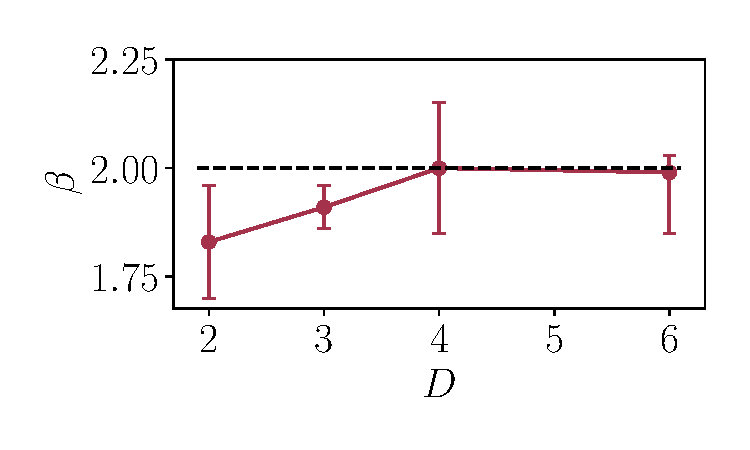
\includegraphics[width=0.5\textwidth]{Chapitre3/Figures/Interpretation/D_dependence.pdf}
	\caption{Evolution de l'exposant critique $\beta$ en fonction de la dimension de l'espace $D$ dans le modèle $\alpha$-ROM avec sauts infinis des particules actives et $\alpha = 0$.}
	\label{fig:Ddep}
\end{figure}

\subparagraph{}Ainsi, dans la limite de grande dimension où la dynamique des particules passives est simplifiée, nous mesurons effectivement $\beta \approx 2$. Malgré le statut fragile de ces résultat, cela suggère que l'image proposée par le modèle $\mu$-Hébraud-Lequeux est effectivement adéquate pour décrire le mécanisme de diffusion des particules passives dans le $\alpha$-ROM dans la limite champ moyen.

\paragraph{Interprétation champ moyen du mécanisme de diffusion en dimension finie}

\subparagraph{}En pratique, les systèmes réels d'intérêt ne se situent pas exactement dans les limites de champ moyen. Toutefois, nous pouvons parfois espérer que le cadre champ moyen associé puisse être capable d'expliquer certains aspects hors de ces limites. Dans cette optique, nous proposons d'étudier le modèle défini précédemment en 2D, dimension d'intérêt pour ce tavail, et pour différentes portées d'interactions $\alpha$. Dans cette version du $\alpha$-ROM, les sauts infinis des particules actives permettent de laisser le contrôle de la criticalité au mécanisme de diffusion, mais dans une limite non-triviale de basse dimension que l'on retrouve dans le $\alpha$-ROM original. Via ces sauts infinis, nous nous attendons à une validité de la relation $\mu = D/\alpha$. Toutefois, la dynamique des particules passives prenant place dans un espace de dimension finie, il est probable que les relations entre les exposants $\mu$, $\theta$ et $\beta$ se voient modifiées. 

\subparagraph{}Pour comprendre ce qu'il subsiste de l'image champ moyen à cette dimension, nous nous concentrons dans ce cas sur les portées $\alpha \in \{ 0.5, 1, 1.25, 1.5, 2, 2.5, 3 \}$, et nous nous intéressons aux exposants $\beta$ puis $\theta$ associés.

\paragraph{Évolution de la convexité}

\label{sec:sautsinfinis}

\subparagraph{}Pour déterminer l'évolution de la convexité dans ce modèle simplifié, nous menons la même analyse que dans le cas du $\alpha$-ROM à la \autoref{sec:TBLRRStat}. Sur la \autoref{fig:mueff}-(a), nous représentons l'évolution de $\beta$ avec l'exposant de portée d'interaction $\alpha$ et, en pointillés noirs, le comportement champ moyen du modèle $\mu$-Hébraud-Lequeux pour $\mu = D/\alpha$. Malgré la dynamique a priori non triviale des particules passives dans le modèle numérique, les deux évolution présentent un très bon accord aux courtes portées $\alpha \gtrsim 1.5$. Plus particulièrement, comme l'image champ moyen le prédit, l'influence du bruit interne sur la criticalité prend place à partir de $\alpha = D = 2$. De manière remarquable, le modèle $\mu$-Hébraud-Lequeux semble donc permettre de rationaliser partiellement la zone continue d'évolution de la criticalité dans ce modèle 2D.

\subparagraph{}Pour les plus grandes portées $\alpha\lesssim 1.5$, si un accord qualitatif est remarqué, le modèle en dimension fini se démarque de l'image champ moyen comme nous le pensions du fait de la dynamique réelle des particules passives.

\begin{figure}[h]
	\centering
	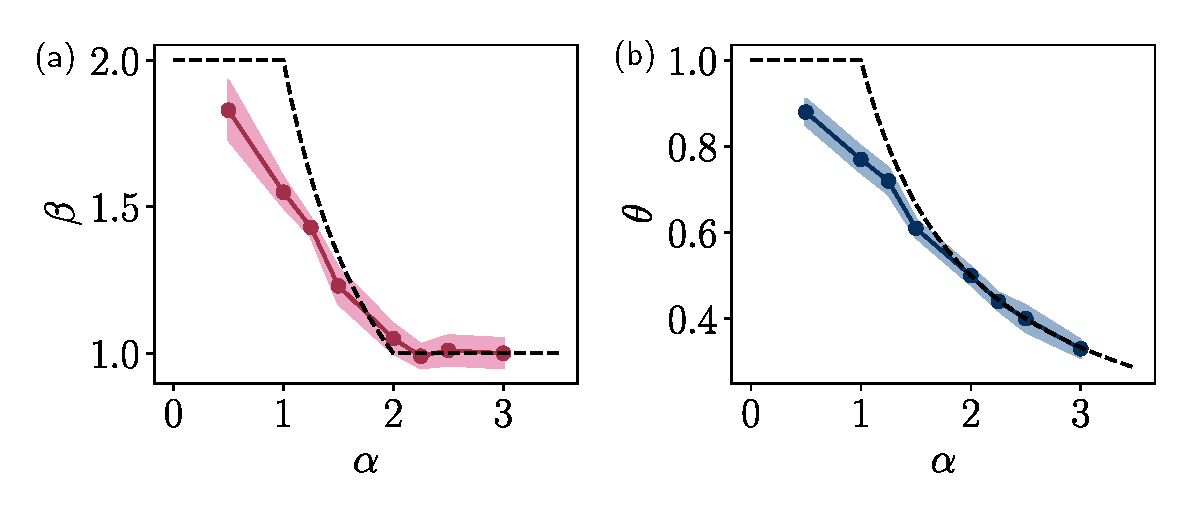
\includegraphics[width=0.8\textwidth]{Chapitre3/Figures/Interpretation/beta_alphaMF.pdf}
	\caption{(a) Evolution de l'exposant $\beta$ avec la portée des interactions $\alpha$ dans le $\alpha$-ROM en 2D avec sauts infinis des particules actives. (b) Idem mais pour l'exposant de pseudo-gap $\theta$. Dans les deux cas, les pointillés noirs représentent les prédictions du modèle $\mu$-Hébraud-Lequeux.}
	\label{fig:mueff}
\end{figure}

\paragraph{Évolution de la distribution des distances à l'activation}

\subparagraph{}Pour tester la pertinence de l'image champ moyen concernant l'exposant $\theta$ dans un cadre de dimension finie, nous proposons tout d'abord une manière de le déterminer dans les modèles numériques dérivés du ROM. Dans le cadre de ces modèles, la distance à l'activation d'une particule peut être associée à la distance à la particule voisine la plus proche. Sous cet angle, la fonction de corrélation de paire entre particules passives $g^p(r)$ semble être l'objet physique le plus adéquat pour caractériser cette propriété. Plus précisément, étant donné que $g^p(r<D_p)=0$ dû à la condition de recouvrement, nous nous attendons à ce que la fonction $g(x) = g^p(r-D_p)$ se comporte comme la distribution $P(R-|\mathbf{r}|)$ du modèle $\mu$-Hébraud-Lequeux. Bien que la fonction de corrélation de paire ne représente pas directement une probabilité de présence du plus proche voisin, nous nous attendons à ce que ce soit le cas asymptotiquement à petits $x$. Ainsi, nous nous attendons, dans le cas idéal où l'image champ moyen est parfaitement retrouvée, à mesurer dans nos simulations numériques au point critique :

\begin{equation}
	g(x) \sim x^\theta, \quad \theta = \left\{
	\begin{aligned}
	&\frac{\mu}{2}, \quad \mu \leq 2\\
	&1, \quad \mu \geq 2
	\end{aligned}
	\right.
	\label{eq:gpass}
\end{equation}

\subparagraph{}Nous proposons alors d'évaluer cet exposant $\theta$ dans le $\alpha$-ROM en 2D avec sauts infinis des particules actives. Nous mesurons donc la fonction de corrélation de paire entre particules passives $g^p(r)$ à petits $r$, pour différentes distances au point critique $\delta\phi$ et ce pour chaque portée $\alpha$. Un exemple de mesures pour $\alpha = 1.5$ et $\alpha = 5$ sont présentées sur les encarts de la \autoref{fig:PCorr_alphaMF}. Une première chose remarquable est que, même si nous considérons un cas de dimension finie ici, nous observons effectivement un comportement algébrique de $g(x)$ avec $x$ qui s'étend à petits $x$ à mesure que le point critique est approché. La prédiction du modèle champ moyen $\mu$-Hébraud-Lequeux quant à une distribution algébrique des distances à l'activation semble donc retrouvée dans ce modèle.

\subparagraph{}\`A très petits $x$, la fonction de corrélation sature sur un plateau dont la valeur décroît avec la distance au point critique. Cela s'explique probablement par le fait que le comportement donné par l'\autoref{eq:gpass} n'est en fait valable qu'au point critique. De ce fait, la détermination directe de l'exposant $\theta$ est rendue difficile, puisque le régime de loi de puissance est parasité par ce plateau. Pour s'affranchir de cet effet, nous utilisons une méthode de redimensionnement par $\delta\phi$ pour mesurer l'exposant $\theta$. Cette méthode est alors très similaire à celle présentée à la \autoref{sec:expdynjump} pour la détermination de l'exposant $\delta$. Pour ce faire, nous supposons donc que la fonction $g^p(x=r-D_p, \delta\phi)$ est homogène de ses arguments dans le régime critique. Dans le cadre de cette hypothèse, en redimensionnant $g^p(x, \delta\phi)$ par $\delta\phi^{a_1}$ et $x$ par $\delta\phi^{a_2}$, il est possible de trouver $a_1$ et $a_2$ tels que les courbes pour différents $\delta\phi$ se superposent toutes sur une courbe maîtresse. Si cette superposition est effectivement réalisable, l'exposant $\theta$ caractérisant le comportement de la fonction avec $x$ est alors directement donné par $\theta = a_1/a_2$.

\begin{figure}[h]
	\centering
	\includegraphics[width=\textwidth]{Chapitre3/Figures/Interpretation/PCorr_alphaMF.pdf}
	\caption{Redimensionnement des fonctions de corrélation de paire des particules passives avec la distance au point critique $\delta\phi$ dans le $\alpha$-ROM avec sauts infinis des particules actives pour $\alpha = 1.5$ (a) et $\alpha=5$ (b). En encart, les données brutes associées. \rem{mettre une flèche pour l'évolution de $\delta\phi$ et les donner en légende}}
	\label{fig:PCorr_alphaMF}
\end{figure}

\subparagraph{}Nous représentons à la \autoref{fig:PCorr_alphaMF} le meilleur redimensionnement par $\delta\phi$ obtenu dans les cas $\alpha = 1.5$ et $\alpha=5$ et reportons le cas des autres portées à la \autoref{sec:PCorr}. Comme on peut le remarquer, la superposition des courbes est remarquablement satisfaisante sous le bon choix d'exposants. Notre hypothèse d'homogénéité de la fonction $g^p(r, \delta\phi)$ est donc bien validée. Une information annexe que nous tirons de ces redimensionnement est que, pour $\theta>0.5$, la valeur au contact $x=0$ de la fonction $g^p$ évolue comme $\delta\phi^{\beta/2}$. De plus, pour $\theta<0.5$, là où nous avons mesuré $\beta=1$, celle-ci évolue comme $\delta\phi^{0.5}$. Ainsi, par définition de l'exposant $\beta$, la valeur du plateau se comporte comme $\sqrt{\langle A \rangle}$ à toute portée. La forme adéquate de la fonction de corrélation de paire à une distance finie du point critique est donc :

\begin{equation}
	g(x) \sim \sqrt{\langle A \rangle} + x^\theta
\end{equation}

\subparagraph{}Pour en revenir à la mesure de l'exposant $\theta$ et son évolution avec la portée, nous traçons sur la \autoref{fig:mueff}-(b) l'évolution de l'exposant $\theta$ mesuré par redimensionnement avec $\alpha$ et, en pointillés noirs, le comportement du modèle $\mu$-Hébraud-Lequeux pour $\mu = D / \alpha$. De manière similaire à l'étude de la convexité, nous remarquons un comportement quantitativement comparable entre le modèle numérique et l'image champ moyen à courte portée $\alpha \gtrsim 1.5$. \`A plus longue portée, nous retrouvons de nouveau un écart avec l'image champ moyen.

\paragraph{Complexité dans la dynamique des particules passives}

\subparagraph{}De manière remarquable, certaines prédictions du modèle champ moyen semblent être vérifiées dans le $\alpha$-ROM avec sauts infinis des particules actives en dimension finie. Notamment, nous retrouvons un impact du mécanisme de diffusion sur la criticalité à partir de $\alpha = D = 2$ et un accord quantitatif sur les courbes $\beta(\alpha)$ et $\theta(\alpha)$ à courte portée. Dans cette partie nous montrons que même si les relations $\beta(\alpha)$ et $\theta(\alpha)$ ne sont plus champ moyen à longue portée, une loi d'échelle du modèle $\mu$-Hébraud-Lequeux reste toujours vérifiée dans ce cas.

\subparagraph{}Les relations $\beta(\alpha)$ et $\theta(\alpha)$ dans le modèle $\mu$-Hébraud-Lequeux sont en fait une combinaison de résultats issus de différentes hypothèses. Elles se basent sur la relation entre $\mu$ et $\alpha$, celle entre $\theta$ et $\mu$, puis celle entre $\beta$ et $\theta$ et $\mu$ \cite{lin_microscopic_2018}. Une manière de tester la pertinence de l'image champ moyen en dimension finie peut être de se concentrer sur une de ces sous-relations, par exemple, la relation d'échelle $\beta = 2\theta$. Sur la \autoref{fig:2thetaMF}, nous superposons donc les évolutions de $2\theta$ et $\beta$ dans le cas du $\alpha$-ROM avec sauts infinis des particules actives. 

\subparagraph{}De manière remarquable, nous observons que la loi d'échelle $\beta = 2\theta$ pour $\theta > 0.5$ est vérifiée à toutes les portées, mêmes les plus grandes où l'accord quantitatif avec le modèle était perdu pour les deux exposants. Ainsi, il semblerait que même dans le domaine où la dynamique des particules passives en dimension finie écarte le modèle numérique de l'image champ moyen, nous retrouvons un lien direct entre la convexité de la transition et la forme de la fonction de corrélation de paire. En ce sens, le modèle $\mu$-Hébraud-Lequeux reste un cadre intéressant pour analyser le mécanisme de diffusion même en dimension finie. Cette observation confirme les résultats préliminaires de la sous-sous-section précédente, plaçant effectivement le modèle $\mu$-Hébraud-Lequeux comme le cadre de description adéquat du mécanisme de diffusion.

\begin{figure}[h]
	\centering
	\includegraphics[width=0.5\textwidth]{Chapitre3/Figures/Interpretation/beta_theta_alphaMF.pdf}
	\caption{Comparaison de l'évolution des exposants $\beta$ et $\theta$ avec la portée $\alpha$ dans le cadre du $\alpha$-ROM en 2D avec sauts infinis des particules actives. La ligne pointillée noire représente $\alpha = 2$ soit $\mu=1$ dans le modèle $\mu$-Hébraud-Lequeux avec $\mu=D/\alpha$}
	\label{fig:2thetaMF}
\end{figure}


\subsubsection{Image champ moyen dans le $\alpha$-ROM}

\subparagraph{}Dans le cadre du $\alpha$-ROM avec sauts finis des particules actives, pour les raisons que nous avons évoqué précédemment, nous ne nous attendons pas à ce que les prédictions de l'image champ moyen puisse se retrouver dans l'analyse du modèle numérique. Toutefois, comme nous le montrons dans cette sous-sous-section, une comparaison avec le modèle $\mu$-Hébraud-Lequeux et avec le modèle numérique avec sauts infinis des particules actives peut amener à des observations intéressantes.

\paragraph{Évolution de la convexité : une influence moindre des corrélations d'activité ?}

\subparagraph{}Sur la \autoref{fig:BetaMu1}-(a), nous comparons les évolutions de l'exposant $\beta$ avec $\alpha$ pour le $\alpha$-ROM en 2D et en 3D avec les prédicitions du modèle $\mu$-Hébraud-Lequeux pour $\mu = D/\alpha$. De manière attendue, nous n'observons d'accord quantitatif dans aucune limite : les mesures numériques présentent systématiquement une convexité moindre. Dans la limite de courte portée, ce désaccord est évident. En effet, dans ce cas là la criticalité est celle de la classe CDP, dominée par la dynamique des particules actives, et n'a donc rien à voir avec le mécanisme proposé par l'image champ moyen. Nous notons toutefois qu'étant donné que l'exposant $\beta_\text{CDP}$ augmente avec la dimension pour arriver à $\beta = 1$ pour $D=4$, en augmentant la dimension, l'écart observable se réduit entre les points de mesure et les pointillés dans la limite gauche du graphique.

\begin{figure}[h]
	\centering
	\includegraphics[width = \textwidth]{Chapitre3/Figures/Interpretation/Beta_Mu1.pdf}
	\caption{(a) Evolution de l'exposant $\beta$ en fonction de $D/\alpha$ dans le $\alpha$-ROM en 2D et en 3D. En pointillés noirs, nous représentons les prédictions du modèle $\mu$-Hébraud-Lequeux. (b) Comparaison de l'évolution de l'exposant $\beta$ avec $\alpha$ dans le cas du $\alpha$-ROM et du $\alpha$-ROM avec sauts infinis des particules actives en 2D.}
	\label{fig:BetaMu1}
\end{figure}

\subparagraph{}Dans la limite de longue portée, cet écart n'est pas non plus surprenant puisque dans la partie précédente concernant le modèle avec sauts infinis des particules actives, nous l'avons attribué à la dynamique des particules passives, qui reste intacte dans le cas du $\alpha$-ROM. Toutefois, nous pouvons noter quelque chose de plus intéressant dans cette zone. Sur la \autoref{fig:BetaMu1}-(b), nous comparons les résultats obtenus en 2D dans le cas de sauts finis et de sauts infinis (resp. activité corrélée et activité décorrélée). Comme nous pouvons le remarquer, à longue portée $\alpha \lesssim 1.25$ les résultats associés aux deux modèles convergent. Cela suggère alors que la dynamique de l'activité n'influence pas, via la modification de la relation $\mu=D/\alpha$ ou via le mécanisme additionnel de création de l'activité par transport, le comportement critique dans cette limite. Ainsi, à longue portée, la création d'activité dans le $\alpha$-ROM semble être dominée par le mécanisme de diffusion (voir \autoref{eq:meca_diff}).

\subparagraph{}Une observation remarquable par ailleurs est que dans le cas $2D$ et $3D$, l'influence des interactions à longue portée sur la criticalité débute en $\alpha = D$, comme le prédit le modèle $\mu$-Hébraud-Lequeux avec $\mu = D/\alpha$, et comme cela a été mesuré dans le cas du modèle avec sauts infinis. 

\paragraph{Évolution de l'exposant de pseudo-gap}

\subparagraph{}Dans la dynamique complexe offerte par le $\alpha$-ROM, dû à la dynamique annexe des particules actives, il n'est pas évident que la fonction de corrélation de paire présente un comportement algébrique comme dans les modèles isolant le mécanisme de diffusion. Pour le vérifier, nous effectuons les mêmes mesures de fonctions de corrélation de paire que dans la partie précédente pour le $\alpha$-ROM en 2D. Simplement, du fait des résultats de l'analyse précédente, nous choisissons de redimensionner directement les quantités par $\langle A \rangle$ et non $\delta\phi$. Les redimensionnements les plus convaincants obtenus sont alors représentés pour $\alpha=0.5$ et $\alpha=1.25$ à la \autoref{fig:PCorr_alpha}. Les autres analyses sont reléguées à la \autoref{sec:PCorr}. 

\begin{figure}[h]
	\centering
	\includegraphics[width=\textwidth]{Chapitre3/Figures/Interpretation/PCorr_alpha.pdf}
	\caption{Redimensionnement des fonctions de corrélation de paire des particules passives avec la distance au point critique $\delta\phi$ dans le $\alpha$-ROM avec sauts finis des particules actives pour $\alpha = 0.5$ (a) et $\alpha=1.25$ (b). En encart, les données brutes associées. \rem{mettre une flèche pour l'évolution de $\delta\phi$ et les donner en légende}}
	\label{fig:PCorr_alpha}
\end{figure}

\subparagraph{}La superposition des courbes est alors toujours satisfaisante, même si un peu moins nette, pour tout $\alpha$. Cela montre que même en présence de la dynamique corrélée des particules actives, les fonctions de corrélation de paire possèdent un caractère non-trivial, signe de la présence du mécanisme de diffusion vers l'activation capturé par l'image champ moyen. Dans le cas de très longue portée, nous retrouvons un comportement en $\sqrt{\langle A \rangle}$ de $g^p(0)$. Toutefois ce comportement semble perdu à plus courtes portées où l'on mesure $g^p(0)\sim A^b$ avec $b>0.5$ dès $\alpha = 1$. En adaptant la méthode de redimensionnement à cette observation, nous sommes capables d'extraire des valeurs de $\theta$ pour chaque $\alpha$. Sur la \autoref{fig:Beta_Theta}, nous représentons l'évolution de $2\theta$ avec $\alpha$ et la mettons en regard de l'évolution de l'exposant $\beta$.

\begin{figure}[h]
	\centering
	\includegraphics[width=0.6\textwidth]{Chapitre3/Figures/Interpretation/Beta_Theta.pdf}
	\caption{Comparaison de l'évolution de $\beta$ et $2\theta$ avec $\alpha$ dans le cas du $\alpha$-ROM en 2D.}
	\label{fig:Beta_Theta}
\end{figure}

\subparagraph{}Nous observons alors une évolution de l'exposant $\theta$ qualitativement en accord avec l'image champ moyen, soit une tendance d'augmentation avec la portée des interactions. Celle-ci semble cependant différente de celle observée dans le cas du modèle à sauts infinis. En effet, l'évolution observée ici est d'une amplitude moindre et nous n'observons par exemple pas de tendance réellement significative dans la zone $1.5 \leq \alpha \leq 2$, là où l'exposant $\beta$ varie pourtant fortement.

\subparagraph{}Si l'on compare les évolutions de $2\theta$ et $\beta$ nous remarquons des divergences claires, signifiant que la relation d'échelle $2\theta = \beta$ n'est plus vérifiée pour tout $\theta > 0.5$. Cette observation est attendue, puisque l'image champ moyen ne permet de toute façon pas de rendre compte d'un exposant $\beta < 1$, ce que l'on a mesuré pour $\alpha \gtrsim 1.5$. Toutefois, de manière remarquable, l'écart entre ces deux exposants se réduit à mesure que la portée augmente, si bien que dans la limite de très grande portée $\alpha = 0.5$ l'accord est retrouvé. Cela conforte l'idée selon laquelle à grande portée, la dynamique de l'activité n'influence plus significativement le comportement critique, faisant du modèle $\mu$-Hébraud-Lequeux le champ moyen adéquat du système même lorsque les particules actives font des sauts finis.

\subsubsection{Conclusion de la sous-section}

\subparagraph{}En conclusion, cette sous-section nous a permis de tester la pertinence de l'image champ moyen pour comprendre le mécanisme de diffusion des particules passives et son influence dans les modèles numériques étudiés. Via l'étude d'une version simplifiée du $\alpha$-ROM, nous avons montré que le modèle $\mu$-Hébraud-Lequeux permet effectivement de rationaliser l'effet du mécanisme de diffusion sur la criticalité malgré la présence d'une dynamique non-triviale des particules passives. 

\subparagraph{}Dans le cas d'une dynamique plus complexe représentée par le modèle $\alpha$-ROM, les prédictions du modèle champ moyen ne tiennent plus de manière générale mais nous permettent de retrouver des traces de l'influence de la diffusion des particules passives. Notamment, nous remarquons une forme algébrique de la fonction de corrélation de paire proche du contact, décrite par un exposant de pseudo-gap $\theta$. De manière remarquable, nous observons par ailleurs que dans la limite de grande portée, la dynamique d'activité dans le modèle ne semble plus contrôler la convexité de la transition, faisant du modèle $\mu$-Hébraud-Lequeux le champ moyen adéquat pour appréhender la dynamique complète.

\subsection{Disqualification complète du cadre LR-CDP}

\subparagraph{}Les analyses précédentes nous ont permis de montrer en quoi la diffusion des particules passives représentait un mécanisme essentiel dans la transition du $\alpha$-ROM. Toutefois, à courte portée au minimum, il ne semble pas que celle-ci suffise à comprendre entièrement la criticalité du modèle. Notamment, les cas où l'on mesure $\beta < 1$ ne peuvent être compris sans les corrélations induites par les sauts des particules actives et le mécanisme de création de l'activité par transport qu'elles représentent. Bien que la zone $\beta >1$ soit hors d'atteinte du cadre de référence LR-CDP, il est tentant de vouloir interpréter cette zone $\beta < 1$ via ce formalisme. Dans ce scénario, le paysage global présenté à la \autoref{sec:TBLRRStat} se formerait donc d'une zone avec $\beta>1$ dominée par la dynamique des particules passives, et d'une zone $\beta<1$ interprétable comme une zone dominée par la dynamique des particules actives.

\subparagraph{}Un premier conflit d'interprétation de cette région concave par ce scénario vient du fait que la zone d'exposant $\alpha$ pour laquelle on passe de $\beta\approx 0.64$ en 2D à $\beta=1$ n'est pas du tout la même que celle du cadre LR-CDP. En effet, nous avons identifié $0.5\lesssim \alpha \lesssim 2$ pour le $\alpha$-ROM et $3<\alpha<4$ pour LR-CDP en 2D. Toutefois, nous pourrions imaginer que le mécanisme de diffusion dans cette zone agisse de la même manière qu'un transport à longue portée, seulement avec un exposant effectif de transport différent. Il serait alors possible de rattacher le $\alpha$-ROM au cadre d'interprétation de l'influence d'un transport à longue portée dans cette zone concave. 

\subparagraph{}Dans le cas d'un transport à longue portée contrôlé par l'exposant $\gamma$, une particule active dans un espace de dimension $D$ fait un saut dont l'amplitude $\Delta$ suit une distribution $P(\Delta)\sim\Delta^{D-1-\gamma}$ (voir \autoref{chapter:TransportLP}). En supposant la densité de particules homogène dans le système, cela correspond pour la particule active à une probabilité $P_a(r)$ de créer de l'activité à une distance $r$ à l’issue du pas de temps telle que :

\begin{equation}
	P_a(r) \sim \frac{1}{r^{1+\gamma-D}}
\end{equation}

\noindent La question est alors de savoir si une telle quantité peut être dérivée dans le cas du $\alpha$-ROM, et comment celle-ci se compare au cas du transport à longue portée à comportement critique équivalent. En d'autres termes, peut-on dériver un exposant de saut effectif $\gamma_\text{eff}$ dans le cadre de ce modèle ? 

\subparagraph{}Pour ce faire, nous considérons la portée $\alpha = 1.75$ pour laquelle nous avions mesuré $\beta\approx 0.82$ dans le $\alpha$-ROM en 2D. Elle se situe donc à mi-chemin entre la limite de courte portée $\beta = 0.64$ et la valeur triviale $\beta = 1$, et donc cette criticalité peut-être atteinte dans le cadre du transport à longue portée. Pour ce faire, nous générons un état absorbant du système à $\phi = \phi_c$. \`A partir de cet état absorbant, nous activons aléatoirement une particule, générant alors un saut de courte portée et un bruit sur toutes les autres particules passives. En identifiant les particules activées suite à ce pas de temps et leur distance $r$ à la particule activée, nous pouvons mesurer la quantité $P_a(r)$ dans ce cadre. Le même protocole peut être appliqué dans le cadre du transport à longue portée. Pour un système de taille $L=4096$, nous comparons alors la mesure de $P_a(r)$ obtenue pour $\alpha = 1.75$ à celle obtenue dans le cas d'un transport à longue portée avec $\gamma = 3.5$. La valeur de $\gamma$ est choisie ainsi puisque dans ce cas nous avions mesuré $\beta \approx 0.81$, soit une valeur très proche de $\beta\approx 0.82$ pour $\alpha = 1.75$ dans le cas du $\alpha$-ROM. Les résultats obtenus sont présentés sur la \autoref{fig:RangeInterpretation}.

\begin{figure}[h]
	\centering
	\includegraphics[width=0.7\textwidth]{Chapitre3/Figures/Interpretation/RangeInterpretation.pdf}
	\caption{Evolution des distributions $P_a(r)$ pour le LR-ROM avec $\gamma = 3.5$ et pour le $\alpha$-ROM avec $\alpha = 1.75$. \todo{Réduire les tailles de police}}
	\label{fig:RangeInterpretation}
\end{figure}

\subparagraph{}Nous constatons alors que dans le cas du transport à longue portée, $P_a(r)$ décroît bien comme $1/r^{2.5}$ en 2D. Dans le cas du $\alpha$-ROM, cette distribution décroît comme $1/r^{1.3}$ soit $\gamma_\text{eff}\approx 2.3$, donc bien moins rapidement. En réalisant ces mêmes mesures sur des états actifs de la dynamique, les mêmes observation peuvent être faites. Ainsi, si les deux modèles partagent le même exposant $\beta$ à ces portées, ils ne partagent pas du tout les mêmes propriétés de création d'activité. En d'autres termes, il ne semble pas possible d'interpréter la criticalité du $\alpha$-ROM via le cadre LR-CDP  dans la zone concave $\beta < 1$. La dynamique des particules passives reste donc importante à toute portée $\alpha < D$ et le changement de convexité ne semble pas relever d'un changement abrupt de mécanisme prépondérant.

\subsection{Conclusion de la section}

\subparagraph{}En conclusion, nous avons établi dans cette section un modèle de type champ moyen permettant une transition de réversibilité convexe. Son étude révèle alors la place essentielle du bruit interne, i.e. de la diffusion des particules passives, dans la criticalité du $\alpha$-ROM. Notamment, dans la limite de très longue portée $\alpha\rightarrow 0$, ce mécanisme de création de l'activité semble pouvoir décrire à lui seul la transition. Enfin, si la zone concave pour laquelle on retrouve $\beta<1$ prend l'apparence du comportement attendu dans le cadre LR-CDP, celle-ci correspond en fait à une dynamique bien différente. In fine, via la présence supplémentaire du mécanisme de diffusion des particules, le modèle $\alpha$-ROM est donc différent en tout point du cadre LR-CDP sous les aspects abordés et nécessite un traitement théorique fondamentalement différent.

\section{Avalanches}

\subparagraph{}Afin de souligner ces différences par un dernier aspect incontournable de la criticalité absorbante, nous proposons d'étudier dans cette section la dynamique d'avalanches à l’œuvre dans le $\alpha$-ROM.

\label{sec:AvSusp}

\subsection{Avalanches à densité fixée}

\subsubsection{Redéfinition}

\subparagraph{}Comme nous l'avons vu au \autoref{chapter:introduction}, les modèles appartenant à la classe CDP présentent une dynamique d'avalanches. Pour la mettre en évidence, il est d'usage de se placer dans le cas de la criticalité auto-organisée (abrégée SOC pour \textit{self-organized criticality}). Dans ce cadre, la séparation d'échelle entre le temps de forçage (ajout de matière aléatoire) et de relaxation (disparition de matière induite par l'activité) permet d'observer distinctement des évènements d'activité fortement corrélés et distribués de manière algébrique : ce sont les avalanches.

\subparagraph{}Une autre manière d'observer la dynamique critique est de se placer dans l'état stationnaire à une densité fixée de particules $\phi$ dans le système, proche de la densité critique $\phi_c$. Le fait est que, dans ces conditions, le système est proche d'une transition de phase absorbante. Ainsi, pour un système de taille finie, du fait des fluctuations de la dynamique, cette dernière peut régulièrement tomber dans un état absorbant pour $\phi \gtrsim \phi_c$. Pour sonder la dynamique d'avalanches à densité imposée, il est donc nécessaire de réactiver le système à chaque fois qu'il se retrouve bloqué. Un protcole généralement utilisé est alors d'activer artificiellement une particule dans le système, alors précurseur de l'évènement \cite{lubeck_universal_2003, vespignani_absorbing_state_2000, munoz_avalanche_1999}.

\subparagraph{}Cette situation impose de redéfinir la notion d'avalanches à densité fixée. Dans ce cadre, nous définissons une avalanche comme l'évènement ayant lieu entre deux réactivations du système. Il est alors possible de définir ces évènements exactement de la même manière que les avalanches de la SOC, i.e. par leur taille $S$, leur durée $T$ et le nombre de particules $N$ qu'ils impliquent. Dans le cadre du $\alpha$-ROM, la taille d'une avalanche correspond au nombre d'évènements d'activité individuels ayant lieu pendant l'évènement global. La durée correspond alors simplement au nombre de pas de temps entre le début et la fin de l'avalanche. Plusieurs études ont montré que ces avalanches étaient de même nature que celles de la SOC dans les modèles à courte portée\footnote{Ces études n'interprétaient cependant pas ces évènements à densité fixée comme des avalanches à proprement parler.} \cite{lubeck_universal_2003, vespignani_absorbing_state_2000, munoz_avalanche_1999}. Il est alors attendu que ces évènements soient aussi distribués de manière algébrique, définis par les exposants d'avalanche déjà présentés à la \autoref{sec:IntroAvalanches} :

\begin{equation}
	\begin{aligned}
		&P(S) \sim S^{-\tau}f\left( \frac{S}{S_c} \right), \quad S_c \sim L^{d_f}\\
		&P(T) \sim T^{-\tau^\prime}g\left( \frac{T}{T_c} \right), \quad T_c \sim L^{z}\\
		&P(N) \sim N^{-\tau^{\prime\prime}}h\left( \frac{N}{N_c} \right), \quad N_c \sim L^{\chi}\\
	\end{aligned}
	\label{eq:AvDistribSusp}
\end{equation}

\subparagraph{}Afin d'analyser le comportement des avalanches à la transition dans le cadre du $\alpha$-ROM, nous choisissons de nous placer à densité fixée. Ce choix se justifie par cohérence, les analyses précédentes ayant toutes été réalisées à densité fixée. Cela nous permet alors de caractériser directement la dynamique qui donne lieu au comportement critique précédemment déterminé.

\subsubsection{Protocole}

\subparagraph{}Pour étudier les avalanches à densité fixée dans le modèle $\alpha$-ROM, pour une portée $\alpha$ donnée, nous nous plaçons à la densité critique $\phi_c$ du système. Dès lors, nous générons un état absorbant du système en partant d'une configuration initiale aléatoire. \`A chaque fois que le système tombe dans un état absorbant, la dynamique est réactivée en activant artificiellement une particule choisie au hasard. Ce processus est alors réitéré suffisamment de fois pour obtenir une statistique propre et stationnaire pour les observables $S$, $T$ et $N$\footnote{En pratique, la stationnarité impose d'ignorer les premiers évènements.}. Nous réalisons alors ces mesures en 2D pour $\alpha \in \{ 3, 2, 1.75, 1.5, 1.25, 0.5\}$ et pour les tailles de systèmes $L \in \{ 256, 512, 1024, 2048 \}$. Un exemple des $3\times 4$\footnote{pour les trois grandeurs $S$, $T$ et $N$ et aux quatre tailles de système.} distributions obtenues est alors présenté à la \autoref{fig:AvSuspNotRescaled} pour $\alpha = 1.5$.

\begin{figure}[h]
	\centering
	\includegraphics[width=\textwidth]{Chapitre3/Figures/Avalanches/Av_alpha15_edited.pdf}
	\caption{Distributions de taille (a), de durée (b) et du nombre de particules impliquées (c) pour les avalanches mesurées dans le modèle $\alpha$-ROM à densité fixée $\phi=\phi_c$ pour $\alpha = 1.5$ et pour $L \in \{ 256, 512, 1024, 2048 \}$.}
	\label{fig:AvSuspNotRescaled}
\end{figure}

\subparagraph{}Les formes des distributions sont alors celles supposées, présentant une décroissance en loi de puissance, commune à chaque taille, puis un cut-off, augmentant avec la taille du système. Par ailleurs, ce cut-off, dans le cas de $P(S)$ et $P(T)$, semble présenter une bosse qui s'étale à mesure que la portée augmente. Afin de déterminer précisément les exposants d'avalanche associés à ces distributions, nous procédons à une analyse d'échelle en taille finie. Pour ce faire, nous reprenons les formes définies par l'\autoref{eq:AvDistribSusp}. Selon ces ansatz, toute la dépendance des distributions en $L$ est portée par le cut-off. Prenons alors l'exemple de la distribution des tailles $P(S)$. En redimensionnant $S$ par $S_c$, nous obtenons :

\begin{equation}
	P(S) \sim L^{-d_f\tau}\tilde{S}^{-\tau}f\left( \tilde{S} \right),  \quad \tilde{S} = \frac{S}{L^{d_f}}
\end{equation}

\noindent Ainsi, en redimensionnant $P(S)$ par $L^{-d_f\tau}$ et $S$ par $L^{d_f}$, les courbes obtenues pour différentes tailles de système $L$ sont indépendantes de $L$, i.e. se superposent. Ce principe constitue alors une méthode graphique de détermination des exposants : les exposants $d_f$ et $\tau$ sont déterminés comme ceux définissant le redimensionnement qui permet la meilleure superposition des courbes obtenues pour différents $L$. Nous représentons alors sur la \autoref{fig:AvSuspRescaled} la meilleure superposition obtenue pour $\alpha = 1.5$. Les représentations graphiques obtenues pour les autres portées sont reportées à la \autoref{sec:AvTBLRRAnnexe} et les exposants ainsi déterminés sont tous reportés dans le \autoref{tab:expocritavsusp}.

\begin{figure}[h]
	\centering
	\includegraphics[width=\textwidth]{Chapitre3/Figures/Avalanches/Rescale_Av_alpha15.pdf}
	\caption{Redimensionnement par $L$ des distributions de taille (a), de durée (b) et du nombre de particules impliquées (c) pour les avalanches mesurées dans le modèle $\alpha$-ROM à densité fixée $\phi=\phi_c$ pour $\alpha = 1.5$ et pour $L \in \{ 256, 512, 1024, 2048 \}$.}
	\label{fig:AvSuspRescaled}
\end{figure}

\subsection{Évolution des exposants}

\subparagraph{}Pour les exposants $\tau$, $\tau^\prime$ et $\tau^{\prime\prime}$, nous observons une tendance d'augmentation avec la portée, comme dans le cadre LR-CDP/depinning (voir \autoref{sec:LRCanonique}). Par exemple, on passe de $\tau\approx 1.28$ pour $\alpha=3$ à $\tau\approx 1.47$ pour $\alpha=1.25$. Nous remarquons par ailleurs que la valeur obtenue à courte portée $\alpha = 3$ est compatible avec les mesures déjà effectuées dans le cas de la classe CDP  \cite{chessa_critical_1999}. Nous notons cependant une anomalie à cette tendance d'augmentation pour $\alpha=0.5$, portée à laquelle le cut-off s'étale le plus sur la loi de puissance. Même si cette tendance générale est modérée, cela montre que les avalanches sont globalement distribuées de moins en moins largement à mesure que la portée des interactions augmente. De ce point de vue, l'évolution est alors compatible avec le cadre LR-CDP, bien que la gamme de portées sur laquelle a lieu l'évolution soit toujours très différente.

\subparagraph{}En contraste, les exposants de structure $d_f$, $z$ et $\chi$ sont soumis à des variations significatives. Dans le cas de la courte portée, pour $\alpha=3$ et $\alpha=2$, nous mesurons $d_f \approx 2.75$, $z\approx 1.55$ et $\chi\approx 2$, soit un parfait accord avec le cas CDP/depinning à courte portée \cite{chessa_universality_1999, lubeck_universal_2004, chessa_critical_1999, wiese_theory_2022, rosso_depinning_2003}. Les études précédentes ayant été menées dans le cadre de la SOC, cela valide l'équivalence avec le cas de densité fixée à courte portée. Nous rappelons par ailleurs qu'obtenir $d_f>D$ dans notre cas n'est pas surprenant puisque la taille $S$ des avalanches caractérise une dynamique en $D+1$ dimensions. 

\begin{table}[h]
\centering
\begin{tabular}{ccccccc}
\hline \hline $\alpha$ & $\tau$ & \multicolumn{1}{c}{$\tau^\prime$} & $\tau^{\prime\prime}$ & $d_f$ & $z$ & $\chi$ \\
\hline 3 & 1.28 & 1.47 & 1.37 & 2.8 & 1.55 & 2 \\
2 & 1.34 & 1.57 & 1.42 & 2.75 & 1.55 & 2 \\
1.75 & 1.41 & 1.72 & 1.47 & 2.4 & 1.30 & 2 \\
1.5 & 1.48 & 1.85 & 1.50 & 2.00 & 1.10 & 2 \\
1.25 & 1.47 & 1.85 & 1.49 & 1.75 & 0.95 & 1.75 \\
0.5 & 1.40 & 1.70 & 1.42 & 1.4 & 0.90 & 1.50\\
\hline \hline
\end{tabular}
\caption{Exposants d'avalanches déterminés dans les modèles $\alpha$-ROM. L'évolution des exposants de structure $d_f$, $z$ et $\chi$ est représentée graphiquement à la \autoref{fig:EvolAvSusp}.}
\label{tab:expocritavsusp}
\end{table}

\subparagraph{}Dès lors que $\alpha < 2$, la dimension fractale associée à ces avalanches diminue, pour atteindre $d_f \approx 1.5$ à $\alpha = 0.5$. Autour du point $\alpha = 1.5$, la dimension fractale des avalanches passe en dessous de la dimension spatiale $D$ du système. Ce point $\alpha = 1.5$ marque donc un changement caractéristique dans la structure des avalanches, qui ne sont alors plus compactes spatialement aux portées plus grandes. Cette observation se confirme par l'évolution de $\chi$, qui caractérise la surface occupée par les avalanches (leur taille spatiale en quelques sortes). En effet, $\chi = D$ signifie qu'au maximum, les avalanches occupent toute la surface du système, elles sont donc compactes spatialement. En revanche $\chi < D$ montre des évènements qui présentent une fractalité spatiale. Le passage de $\chi\approx 2$ pour $\alpha\geq 1.5$ à $\chi < 2$ pour $\alpha < 1.5$ montre donc bien une perte en compacité spatiale des évènements autour de $\alpha = 1.5$.

\subparagraph{}L'exposant dynamique $z$ diminue lui aussi avec la portée pour $\alpha<2$. Il effectue un changement notable autour de $\alpha = 1.5$ puisqu'il passe de $z>1$ à $\alpha=1.5$ à $z<1$ à $\alpha=1.25$. Cette diminution de $z$ avec la portée correspond par ailleurs à l'attendu LR-CDP/depinning. En effet, si l'on suppose que la relation de scaling $z = \frac{\nu_\parallel}{\nu_\perp}$ est vérifiée dans notre cadre d'étude \cite{lubeck_universal_2004}, alors nous nous attendons bien à ce que $z$ diminue avec la portée puisque $\nu_\perp$, lui, augmente (voir \autoref{chapter:TransportLP}).

\begin{figure}[h]
	\centering
	\includegraphics[width=\textwidth]{Chapitre3/Figures/Avalanches/Recap_AvSuspensions.pdf}
	\caption{Evolution des exposants de strcucture des avalanches $d_f$, $z$ et $\chi$ avec la portée $\alpha$ dans le modèle $\alpha$-ROM en 2D.}
	\label{fig:EvolAvSusp}
\end{figure}

\subparagraph{}Finalement, les propriétés d'avalanches du $\alpha$-ROM suivent une évolution similaire à celle des exposants critiques. Pour $\alpha \gtrsim 1.5$, l'évolution observée est celle convenue dans le cadre LR-CDP/depinning pour les exposants $\tau$, $\tau^\prime$, $\tau^{\prime\prime}$ et $d_f$ avec des évènements spatialement compacts $\chi=D$. Pour $\alpha\lesssim 1.5$ cependant, nous observons un comportement hors des bornes du cadre LR-CDP avec des avalanches spatialement fractales.

\section{Conclusion}

\subparagraph{}En conclusion, nous avons caractérisé dans ce chapitre l'influence des interactions médiées sur la transition de réversibilité des suspensions cisaillées cycliquement. Cette caractérisation s'est faite via la définition d'un modèle numérique baptisé $\alpha$-ROM en deux et trois dimensions, contrastant avec le modèle de transport à longue portée LR-ROM établi au chapitre précédent. Celle-ci a alors montré des différences fondamentales entre le comportement critique observé et celui attendu dans le cadre théorique LR-CDP.

\subparagraph{}En déterminant les exposants critiques statiques et dynamiques associés, nous avons mis en évidence l'influence de la portée des interactions sur le comportement critique. Cette influence prenant alors place sur une gamme de portée disjointe de celle dans le cadre LR-CDP. De plus, nous avons identifié une gamme de portées sur laquelle la transition se révèle convexe ($\beta >1$) et les fluctuations évanescentes ($\gamma^\prime < 0$), rejoignant alors le modèle de portée infini initialement proposé par Mari et al. \cite{mari_absorbing_2022}.

\subparagraph{}Ces observations nous ont poussé à définir un nouveau cadre théorique pour décrire la transition de réversibilité en présence d'interactions médiées. Nous avons alors établi un modèle champ moyen baptisé $\mu$-Hébraud-Lequeux, permettant de rendre compte de la convexité de la transition via la dynamique des particules passives et de comprendre dans une limite champ moyen l'influence de la portée des interactions sur le comportement critique.

\subparagraph{}Enfin, nous avons caractérisé cette famille de transitions par sa dynamique d'avalanches. En réalisant des avalanches à densité de particules fixées, nous avons montré que leur statistique dépend fortement de la portée de l'interaction étudiée. Notamment, les exposants d'avalanche suivent une évolution proche des exposants critiques statiques, délimitant une zone fondamentalement différente du cadre LR-CDP. Dans cette zone de portée où les avalanches dans le cadre LR-CDP ont déjà atteint le régime de champ moyen, les avalanches dans le cadre du modèle $\alpha$-ROM montrent une structure spatialement fractale.
\chapter{Transition vers l'écoulement des fluides à seuil}

\label{chapter:yielding}

\subparagraph{}Dans le \autoref{chapter:introduction}, nous avons vu que la transition vers l'écoulement peut être comprise comme une transition de phase absorbante. Le paramètre de contrôle est alors la contrainte imposée au système $\Sigma$ et le paramètre d'ordre le taux de déformation $\dot{\gamma}$. Ce dernier est nul dans la phase absorbante pour $\Sigma < \Sigma_c$ et non-nul dans la phase active pour $\Sigma > \Sigma_c$. Proche de la transition, l'évolution de $\dot{\gamma}$, de sa variance $\langle\Delta\dot{\gamma}^2\rangle$ et de la longueur de corrélation $\xi$ sont dictées par les exposants critiques $\beta, \gamma^\prime$ et $\nu_\perp$ selon :

\begin{equation}
	\dot{\gamma} \sim \delta\Sigma^\beta,\quad \langle\Delta\dot{\gamma}^2\rangle \sim \delta\Sigma^{-\gamma^\prime}, \quad \xi \sim \delta\Sigma^{-\nu_\perp}, \quad \delta\Sigma = \frac{\Sigma-\Sigma_c}{\Sigma_c}
\end{equation}

\noindent avec la spécificité $\beta>1$ qui rend cette transition très différente de celle qui lui est souvent associée, la transition de dépiégeage, pour laquelle on trouve $\beta \leq 1$. La transition de dépiégeage étant elle-même associée à la criticalité LR-CDP (ou CDP dans le cas d'élasticité à courte portée), cette observation place la transition vers l'écoulement hors de ce cadre théorique. 

\subparagraph{}La spécificité de la transition vers l'écoulement et sa différence avec le cadre LR-CDP sont attribuées à la présence d'un bruit mécanique dans le système. Celui-ci, issu des interactions de signe alterné de Eshelby que nous avons évoquées au \autoref{chapter:introduction}, change la manière d'appréhender le système en apportant un nouveau mécanisme de création de l'activité par diffusion sous influence non-locale de l'activité, et non par transport à longue portée sous influence locale de l'activité (voir \autoref{chapter:introduction}). Dans ce cadre, les modèles théoriques de Hébraud-Lequeux et ses généralisations que nous avons réutilisés pour l'interprétation de la transition de réversibilité au  \autoref{chapter:Susp} permettent de rendre compte de la convexité de la transition vers l'écoulement. Toutefois, toutes les études réalisées dans le cadre de la transition vers l'écoulement se concentrent spécifiquement, et à raison, sur le cas d'une redistribution élastique de la contrainte, soit décroissant comme $\sim 1/r^\alpha$ avec $\alpha = 2$ en 2D. Afin de proposer une comparaison riche entre cette transition et la transition de réversibilité, il s'avère donc intéressant d'étudier de la même manière l'évolution de sa criticalité en fonction de la portée des interactions $\alpha$. Le but de ce chapitre est alors de réaliser une étude numérique similaire à celle du chapitre précédent afin de resituer la transition vers l'écoulement dans une image plus globale que celle proposée par les modèles champ moyen de type Hébraud-Lequeux. Cela nous permettra alors, au chapitre suivant, de disposer de plus d'éléments pour discuter des similarités et des différences entre la transition de réversibilité et la transition vers l'écoulement.

\subparagraph{}Pour ce faire, nous présenterons d'abord la méthode numérique élastoplastique utilisée pour simuler la transition vers l'écoulement en 2D. Ensuite nous mettrons en application cette méthode pour déterminer les exposants critiques associés dans le cas des interactions élastiques d'Eshelby pour lesquelles on a $\alpha=2$. Puis en modifiant la portée des interactions dans le modèle de base, nous caractériserons l'évolution de cette criticalité avec $\alpha$. Enfin, nous complèterons cette première caractérisation via l'évolution des autres propriétés critiques du système comme l'hyperuniformité et la dynamique d'avalanche.

\section{Étudier la transition vers l'écoulement des fluides à seuil}

\subparagraph{}La transition vers l'écoulement, même si non-systématiquement abordée en tant que transition de phase absorbante, reste un objet d'étude central en matière molle. Notamment, beaucoup se sont intéressé-es à la forme de la courbe d'écoulement associée $\dot{\gamma} = f(\Sigma)$ et de sa potentielle universalité. Un modèle phénoménologique communément utilisé pour la décrire est celui d'Herschel-Bulkley \cite{herschel_konsistenzmessungen_1926} :

\begin{equation}
	\dot{\gamma} = k(\Sigma-\Sigma_c)^{1/n},\quad k,n > 0
\end{equation}

\noindent Cette forme est alors tout à fait équivalente à la description en termes de phénomène critique, avec l'exposant $\beta$ relié à l'exposant d'Herschel-Bulkley par $\beta = 1/n$. Par la mesure de $n$ sur différents systèmes, les chercheur-euses ont alors questionné l'universalité de cette courbe. Cela revient donc à explorer un aspect de la criticalité de cette transition. Ces études peuvent alors nous guider sur la méthode la plus adaptée pour explorer plus largement et précisément cette criticalité.


\subsection{Expérimentalement}

\subparagraph{}Expérimentalement, l'exposant de Herschel-Bulkley a été mesuré dans de nombreux systèmes. Que ce soit dans les monocouches de mousse \cite{katgert_flow_2009}, les émulsions \cite{becu_yielding_2006, jop_microscale_2012}, les suspensions colloïdales \cite{ovarlez_rheopexy_2013} ou les verres de colloïdes \cite{besseling_three_dimensional_2007}, des exposants allant de $n\approx 0.4$ à $n\approx 0.7$ ont pu être mesurés. Même si les mesures se montrent souvent dépendantes de certaines propriétés du système, la grande majorité soulignent un caractère convexe de la courbe d'écoulement avec $n<1$ et donc $\beta>1$. Dans certains cas cependant, la propriété de fluide à seuil ou la monotonicité de la courbe d’écoulement peuvent être perdues par une faible modification des propriétés microscopiques du système \cite{becu_yielding_2006}. De plus, les mesures de la contrainte et du taux de déformation peuvent être grandement affectées par des effets parasites comme les glissements à l'interface \cite{bonn_yield_2017}.

\subparagraph{}Ainsi, si les expériences d'écoulement des fluides à seuil en laboratoire révèlent une certaine universalité via la relation d'Herschel-Bulkley, leur exécution peut être soumise à de nombreuses contraintes réelles et à l'interférence de mécanismes supplémentaires. Le but de notre étude étant de se focaliser sur le concept global du phénomène d’écoulement, il peut être avantageux de travailler dans des situations idéalisées pour une analyse précise et simplifiée.


\subsection{Numériquement}

\subparagraph{}L'outil numérique apparaît alors comme une évidence pour étendre cette étude. Via les méthodes de dynamique moléculaire, il est possible de simuler des écoulements amorphes à différents degrés de modélisation. Des comportements similaires aux expériences ont  alors pu être observés, même à de très petites échelles, souvent moins accessibles en laboratoire. Un problème soulevé par ces études est que, dans de tels systèmes, l'agitation thermique peut jouer un rôle essentiel sur la transition, modifiant de fait la courbe d'écoulement \cite{delbecq_rheological_2023} et donc toute la criticalité. Afin d'étudier le phénomène dans sa forme la plus simple possible, nous choisissons de nous limiter dans ce travail au cas athermique. Cela signifie que l'agitation thermique est considérée négligeable, sans impact sur le comportement critique. 

\subparagraph{}Cette simplification n'exclut cependant pas la modélisation de tous les systèmes à petites échelles car ces derniers peuvent s'avérer effectivement athermiques sous certaines conditions. Par exemple, un exposant $n\approx 0.5$ est retrouvé pour le régime athermique du silicone amorphe dans \cite{fusco_rheological_2014}. Les méthodes moléculaires permettent donc de retrouver les résultats expérimentaux dans des conditions plus contrôlées. 

\subparagraph{}En revanche, un problème de ces méthodes est leur fort coût numérique qui rend impossible l'étude de très grands systèmes. Or les phénomènes critiques étant décrits aux grandes échelles, cela représente un obstacle de taille pour la caractérisation de la transition vers l'écoulement des fluides à seuil athermiques. Un autre point plus fondamental qui rend ces modèles inadéquats pour notre caractérisation est que ceux-ci font intervenir un grand nombre de paramètres (forme du potentiel d'interaction, ...) qui dépendent du système spécifique considéré. Dans le but de mettre en évidence une universalité dans le phénomène d'écoulement, il est plus adapté de se concentrer sur des modélisations minimales.


\subsection{Théoriquement}

\subparagraph{}Une manière de répondre à cette difficulté est de s'appuyer sur une approche théorique générale, reposant sur la phénoménologie essentielle du phénomène.

\subsubsection{Groupe de renormalisation et difficultés}

\label{sec:TheoEPM}

\subparagraph{}Dans le cas des phénomènes critiques, ces approches théoriques se basent en général sur les théories de champ et les outils du groupe de renormalisation. Notamment, dans le cas de la transition de dépiégeage, les méthodes du groupe de renormalisation fonctionnel permettent de prédire l'équivalent de la courbe d'écoulement du système ($v(f_\text{ext})$, voir \autoref{chapter:introduction}) proche de la transition. Toutefois, même si des études ont tenté de décrire la transition vers l'écoulement dans le même formalisme que celui du dépiégeage \cite{tyukodi_depinning_2016}, une différence fondamentale bloque l'application de ces méthodes dans notre cas. En fait, là où le propagateur de redistribution dans le cas du dépiégeage est positif en tout point, dans le cas de la transition vers l'écoulement, celui-ci change de signe. En effet, comme nous l'avons vu au \autoref{chapter:introduction}, l'interaction de redistribution d'Eshelby, lors d'un réarrangement plastique, stabilise aussi bien qu'elle ne déstabilise le reste du matériau. Au contraire, dans le cas de la transition de dépiégeage, le dépiégage d'une zone entraîne nécessairement la déstabilisation des autres zones.

\subparagraph{}Cette différence physique a souvent été mise en avant pour expliquer les différences existantes entre transition de dépiégeage et transition vers l'écoulement \cite{lin_scaling_2014,lin_mean-field_2016,nicolas_deformation_2018, ferrero_elastic_2019}. En effet, c'est elle qui est à l'origine de la compréhension des interactions de redistribution dans la transition vers l'écoulement comme un bruit mécanique. Pour conserver une approche théorique, il faut donc se baser sur de nouvelles méthodes de description. Une voie s'ouvre alors sur des approches de type champ moyen, dont l'une des plus célèbres est le modèle de Hébraud-Lequeux.

\subsubsection{Modèle de Hébraud-Lequeux et généralisation}

\label{sec:HL_def}

\subparagraph{}Le modèle de Hébraud-Lequeux \cite{hebraud_mode_coupling_1998} est un modèle qui permet de prédire certaines propriétés de la transition vers l'écoulement, notamment la forme de la courbe $\dot{\gamma} = f(\Sigma)$. Ce modèle se base en fait sur la phénoménologie présentée au \autoref{chapter:introduction}. Considérant le matériau comme un ensemble de régions distinctes portant chacune une contrainte locale $\sigma$ et soumises à un taux de cisaillement $\dot{\gamma}$, la distribution de probabilité $P(\sigma)$ se voit régie par l'évolution :

\begin{equation}
\begin{aligned}
	\partial_t P(\sigma, t) &= -\dot{\gamma}\partial_\sigma P(\sigma, t) + a\Gamma(t)\partial_\sigma^2P(\sigma, t) - \frac{\Theta (|\sigma|>\sigma_Y)}{\tau}P(\sigma, t) + \Gamma(t)\delta(\sigma)\\
	\Gamma(t) &= \frac{1}{\tau}\int_{|\sigma|>\sigma_Y}\mathrm{d}\sigma ~ P(\sigma, t)
\end{aligned}
\label{eq:HLchap4}
\end{equation}

\noindent avec $\tau$ un temps caractéristique de relaxation et $a$ un paramètre du modèle aussi appelé fluidité. Le premier terme du membre de droite de l'\autoref{eq:HLchap4} représente alors le chargement élastique du matériau. Le troisième et le dernier terme représentent le phénomène de relaxation locale lorsque la région dépasse sa contrainte seuil $\sigma_Y$ et opère un réarrangement plastique. Toute la physique capturée dans le modèle réside alors dans le second terme de diffusion. Celui-ci modélise l'influence des régions en réarrangement sur les autres régions via les interactions élastiques d'Eshelby. Cette interprétation vient du fait que ces interactions sont de signe alterné et donc, dans une certaine mesure, représentent une sorte de bruit mécanique dans le matériau. L'intensité de ce bruit dépend alors proportionnellement de la proportion de régions en réarrangement dans le système $\Gamma (t)$.

\subparagraph{}En résolvant ce système d'équations simples dans la limite stationnaire pour $a < \frac{\sigma_Y^2}{2}$, il est possible de déduire une relation entre la contrainte moyenne $\langle \sigma \rangle =  \int \mathrm{d}\sigma ~ \sigma P(\sigma)$ et le taux de cisaillement lorsque $\dot{\gamma}\rightarrow 0$ \cite{olivier_fluides_2011, bertin_stochastic_2022} :

\begin{equation}
	\dot{\gamma} \sim (\langle \sigma \rangle - \Sigma_c)^\beta, \quad \beta = 2
\end{equation}

\noindent On retrouve alors une forme de type Herschel-Bulkley avec $n=0.5$, prédiction proche des résultats expérimentaux et numériques. Ce modèle simple permet donc de rendre compte de la convexité de la transition vers l'écoulement. Il se démarque alors des approches classiques de théorie des champs comme celle associée à la classe CDP ou à la transition de dépiégeage en proposant une description statistique à l'échelle mésoscopique. 

\subparagraph{}Toutefois, ce modèle reste très simplificateur et ne permet pas de rendre compte de toutes les propriétés critiques associées à la transition. Des approches de généralisation de ce modèle ont été étudiées \cite{agoritsas_relevance_2015, bouchaud_spontaneous_2016}, notamment en complexifiant la forme du bruit mécanique afin de rendre compte de la spatialisation des interactions d'Eshleby \cite{lin_mean-field_2016, lin_microscopic_2018}, comme nous l'avons évoqué au \autoref{chapter:Susp}. Ces études sont intéressantes d'un point de vue champ moyen notamment car elles permettent une interprétation de l'évolution des propriétés de la transition avec la portée des interactions. Cependant, elles ne permettent pas d'accéder à certaines quantités comme les fluctuations critiques et les corrélations spatiales proche de la contrainte seuil. Afin d'étudier pleinement cette transition en dimension finie et toute la richesse qui y est associée, il est donc nécessaire d'effectivement spatialiser ce type de description. 

\section{Les modèles élastoplastiques comme outils privilégiés}

\subparagraph{}L'approche idéale pour l'étude de la transition vers l'écoulement des fluides à seuil athermiques semble alors se situer entre une description microscopique réaliste et spatialisée, mais coûteuse, et une description phénoménologique macroscopique, mais trop simplificatrice. Les modèles élastoplastiques répondent alors parfaitement à ce besoin. Nous présentons la méthode utilisée dans ce travail pour caractériser la transition.

\subsection{Principe d'un modèle élastoplastique}

\subparagraph{}Comme expliqué dans le \autoref{chapter:introduction}, l'écoulement des fluides à seuil consiste en une succession d'évènements plastiques locaux, lesquels s'entre-déclenchent les uns les autres. Afin de modéliser ce comportement spécifique tout en conservant une efficacité de calcul satisfaisante et une modélisation très générique du phénomène, les modèles élastoplastiques se basent sur une description mésoscopique du matériau étudié \cite{nicolas_deformation_2018}. Conceptuellement, le matériau est découpé en une collection de sites représentant chacun un groupe de particules susceptible d'effectuer un réarrangement plastique (voir \autoref{fig:mesoscale}). En pratique ces sites peuvent donc représenter quelques constituants élémentaires, comme dans le cas des mousses \cite{schott_multiscale_2024}, ou quelques centaines d'entre eux, comme dans le cas des verres métalliques \cite{pan_experimental_2008}.

\subparagraph{}Dans la description élastoplastique, on associe à chacun de ces sites indexé par un indice $i$ une contrainte tensorielle locale $\bar{\bar{\sigma}}_i$. Afin de simplifier au maximum la modélisation du phénomène d'écoulement, nous considérons dans la suite de ce travail le cas simple d'un matériau bidimensionnel situé dans le plan $(\mathbf{e}_x, \mathbf{e}_y)$ et cisaillé dans la direction $\mathbf{e}_x$. Dans ce cas, il est d'usage de se concentrer sur une unique composante $\sigma_{xy}$ du tenseur afin de rendre la description scalaire et de considérer les réarrangements plastiques comme ayant tous la même symétrie que le forçage \cite{picard_slow_2005, liu_driving_2016, lin_scaling_2014, ferrero_criticality_2019}. Ainsi, chaque site $i$ porte une contrainte $\sigma_i\equiv\sigma_{xy,i}$ constituante de la contrainte globale imposée au système $\Sigma = \frac{1}{N}\sum_{i}\sigma_i$, avec $N$ le nombre de sites. En notant $\mu$ le module de cisaillement associé au matériau étudié, on peut associer de la même manière une déformation élastique $\epsilon_{\text{él},i}$ à chaque site selon $\epsilon_{\text{él},i} = \sigma_i/\mu$. 

\begin{figure}[h]
	\centering
	\includegraphics[width=0.8\textwidth]{Chapitre4/Figures/Methode/Mesoscaling.pdf}
	\caption{Représentation schématique du principe des modèles élastoplastiques. Chaque groupe de particules dans la vision microscopique est représenté par un site pouvant prendre deux états : élastique ou plastique.}
	\label{fig:mesoscale}
\end{figure}

\subparagraph{}Chaque site possède un seuil de contrainte microscopique local $\sigma_{Y,i}$ qu'il est capable de soutenir élastiquement. Mais dès lors que la contrainte locale excède ce seuil local ($\sigma_i > \sigma_{Y,i}$), le site devient à même d'opérer un réarrangement plastique. Ce processus intervient selon un temps caractéristique $\tau_{\text{pl}}$. Quand le réarrangement se produit, le site passe alors dans un état plastique ($n_i = 1$) et accumule une déformation plastique $\epsilon_{\text{pl},i}$ sur un temps caractéristique $\tau$. Cette déformation plastique permet alors une relaxation de la contrainte locale proportionnellement. La relaxation a lieu sur temps caractéristique $\tau_{\text{él}}$ après lequel le site retrouve son état élastique ($n_i = 0$).

\subparagraph{}Durant la relaxation, la contrainte accumulée par le site est redistribuée aux autres sites constituant le matériau via les interactions élastiques d'Eshelby, dont la forme est rappelée à la \autoref{fig:resultsimplem}-(a). Dans l'hypothèse que nous choisissons où les réarrangements plastiques présentent tous la même symétrie que le forçage, les propagateurs de Eshelby ont une orientation fixe, dans le sens du réseau. Cette redistribution va alors potentiellement permettre à d'autres sites de dépasser à leur tour leur seuil local et ainsi opérer un réarrangement. C'est cette interaction de redistribution et ces réarrangements en chaîne qui sont à l'origine du comportement collectif d'écoulement plastique du matériau.

\subparagraph{}Les règles précises qui définissent la co-évolution des variables $(\sigma_i, \epsilon_{\text{pl},i}, n_i)$ sur chaque site dépendent alors du modèle spécifique considéré.

\subsection{Le modèle de Picard}

\subparagraph{}Le modèle élastoplastique retenu pour mener notre étude est le modèle de Picard \cite{picard_slow_2005}. Ce modèle pionnier du domaine est reconnu pour sa simplicité. C'est alors un outil de choix pour étudier ce système du point de vue des transitions de phase absorbantes.

\subparagraph{}Dans le modèle de Picard, tous les sites composant le matériau, indexés $i$ et situés en $\mathbf{r}_i$, possèdent un seuil local identique et constant dans le temps $\sigma_{Y,i}=\sigma_Y$. Dès lors que son seuil est dépassé, un site devient plastique avec un taux de transition constant $1/\tau_ {\text{pl}}$. Une fois plastique, ce site retrouve sa forme élastique avec un taux $1/\tau_ {\text{él}}$. L'évolution de la contrainte locale d'un site isolé prend alors la forme illustrée sur la \autoref{fig:rules}.

\begin{figure}[h]
	\centering
	\includegraphics[width=0.5\textwidth]{Chapitre4/Figures/Methode/PicardTau.pdf}
	\caption{Représentation schématique de l'évolution de la contrainte locale dans le modèle de Picard pour un site isolé.}
	\label{fig:rules}
\end{figure}

\subparagraph{}Pour simplifier davantage cette approche, nous choisissons d'uniformiser les échelles de temps de telle manière que $\tau_{\text{pl}} = \tau_{\text{él}} = \tau$. On peut alors résumer ce modèle par le système d'équations suivant :

\begin{equation}
	\partial_t\sigma_i = 2\mu\sum_{j}G_{ij}\partial_t \epsilon_{pl,j},\quad \partial_t \epsilon_{pl,i} = \frac{1}{2\mu\tau}n_i \sigma_i,\quad
	\left\{
    \begin{array}{lcc}
    n_i: & 0\xrightarrow{\tau}1 & |\sigma_i|>\sigma_\mathrm{Y} \\
    n_i: & 0\xleftarrow{\tau}1 & \forall \sigma_i\\
    \end{array}
    \right.
\label{eq:PicardRules}
\end{equation}

\noindent avec $G_{ij} = G(\mathbf{r}_i-\mathbf{r}_j)$ le noyau de redistribution en champ lointain d'Eshelby  défini au \autoref{chapter:introduction} et décrit en coordonnées polaires par $G(r,\theta) = \frac{\cos 4\theta}{\pi r^2}$. Cette description peut aisément se généraliser en trois dimensions mais notre étude s'est concentrée uniquement sur le cas bidimensionnel. Afin de simplifier l'implémentation numérique, ce système d'équations est adimensionné par les transformations :

\begin{equation}
	\tilde{\sigma_i} = \frac{\sigma_i}{\sigma_Y},\quad \tilde{t} = \frac{t}{\tau}, \quad \tilde{\epsilon}_{pl,i} = \frac{2\mu\tau}{\sigma_Y}\epsilon_{pl,i}
	\label{eq:PicardDim}
\end{equation}

\noindent pour obtenir :

\begin{equation}
	\partial_t\tilde{\sigma}_i = \sum_{j}G_{ij}\partial_t \tilde{\epsilon}_{pl,j},\quad \partial_t \tilde{\epsilon}_{pl,i} = n_i \tilde{\sigma}_i,\quad
	\left\{
    \begin{array}{lcc}
    n_i: & 0\xrightarrow{\tau}1 & |\tilde{\sigma}_i|>1 \\
    n_i: & 0\xleftarrow{\tau}1 & \forall \tilde{\sigma}_i\\
    \end{array}
    \right.
\label{eq:PicardRulesAdim}
\end{equation}

\noindent et nous omettrons le $\tilde{}$ pour alléger les notations dans la suite.

\subparagraph{}Il semble par ailleurs important de mentionner que la simplicité de ce modèle n'enlève rien à son pouvoir descriptif. En effet, pour les quantités et les phénomènes sur lesquels nous allons nous concentrer ici (exposants critiques, avalanches, ...) le modèle de Picard reproduit à l'identique les résultats des modèles plus raffinés \cite{ferrero_criticality_2019}, notamment ceux conservant une description tensorielle complète \cite{nicolas_deformation_2018, budrikis_universal_2017}.

\subsection{Implémentation numérique}

\subparagraph{}Afin de simuler l'écoulement cisaillé représenté par ce modèle, nous reprenons un code mis au point précédemment dans l'équipe PSM du LIPhy que nous modifions selon notre besoin. $N$ sites sont positionnés sur une grille carrée périodique de taille $L\times L = N$ et d'axes principaux $(\hat{\mathbf{e}}_x, \hat{\mathbf{e}}_y)$. La position de chaque site est alors donnée par $\mathbf{r}_i = na\hat{\mathbf{e}}_x + ma \hat{\mathbf{e}}_y$ avec $(n,m) \in \mathbb{N}^2$ et $a$ le pas du réseau que l'on prend égal à 1. En pratique, nous considérons la règle d'évolution directement sous sa forme intégrée :

\begin{equation}
	\sigma_i(t) = \sigma_{\text{int},i}(t)+\sigma_\text{ext} =  \sum_{j}G_{ij}\epsilon_{\text{pl},j}(t)+\Sigma
	\label{eq:DynPicardInteg}
\end{equation}

\noindent et l'évolution de $\epsilon_{\text{pl},j}$ donnée par l'\autoref{eq:PicardRulesAdim} est discrétisée dans le temps, calculée sur chaque site tous les $\Delta t = 10^{-2}~\tau$ selon une méthode d'Euler. \`A chaque pas de temps, les sites élastiques ($n_i=0$) au-dessus du seuil microscopique ($\sigma_i >1$) ont une probabilité $\Delta t / \tau$ de devenir plastiques tandis que les sites plastiques ont la même probabilité de redevenir élastiques.

\subparagraph{}Le point clé de l'algorithme est alors le calcul de la convolution $\sum_{j}G_{ij}\epsilon_{\text{pl},j}$ puisqu'elle admet naïvement une complexité d'ordre $N^2$. Afin d'optimiser nos calculs, nous tirons parti du fait que les sites soient disposés sur une grille régulière. Cela nous permet de déterminer ce terme selon une méthode pseudo-spectrale : la convolution est calculée dans l'espace de Fourier discret où elle devient le simple produit $\hat{G}(\mathbf{q})\hat{\epsilon}_{\text{pl}}(\mathbf{q})$ puis l'on revient à sa représentation dans l'espace réel par une transformée de Fourier inverse discrète. Pour ce faire, nous implémentons directement le propagateur de Eshelby dans sa forme spectrale discrète \cite{picard_elastic_2004} :

\begin{equation}
	\hat{G}(\mathbf{q}) = -4\frac{q_x^2 q_y^2}{q^4}, \quad (q_x, q_y) = \frac{2\pi}{L} \times (n,m)
	\label{eq:eshelbydiscretfourier}
\end{equation}

\noindent avec $\hat{G}(\mathbf{q}=0) = 0$ afin de conserver la contrainte totale du système. L'optimisation des algorithmes de FFT permet alors de réduire la complexité à l'ordre $N\log(N)$ \cite{cooley_algorithm_1965}. De plus, l'analyse de Fourier permet de prendre en compte les limites périodiques de manière naturelle. Le schéma de calcul devenant complètement parallélisable, il est implémenté sur des cartes graphiques via le langage CUDA \cite{cuda} afin d'optimiser nettement la rapidité d'exécution des simulations. Grâce à ces ajustements, nous sommes capables de simuler le comportement de systèmes dont la taille va de $L=32$ à $L=2048$\footnote{L'algorithme de FFT étant optimisé pour des tailles de la forme $2^n$ avec $n\in\mathbb{N}$, nous privilégions ces tailles pour les simulations.}.

\subparagraph{}En pratique, le système est d'abord cisaillé sous une forte contrainte globale $\Sigma_\text{preshear}$ durant un temps $T_\text{preshear}$ avant d'être soumis brutalement à la contrainte globale souhaitée $\Sigma$. Le système évolue alors jusqu'à un état stationnaire caractérisé par une valeur moyenne du taux de déformation $ \dot{\gamma}  = \frac{1}{N}\sum_{i}\partial_t\epsilon_{pl,i}$ (voir \autoref{fig:resultsimplem}-(b)), nulle pour $\Sigma<\Sigma_c$ et positive pour $\Sigma>\Sigma_c$. Nous sommes alors capables avec ce modèle de tracer la courbe d'écoulement $\langle \dot{\gamma} \rangle = f(\Sigma)$ représentée sur la \autoref{fig:resultsimplem}-(c), qui montre clairement la convexité de la transition, par opposition à la concavité de celle de la transition de dépiégeage. En étudiant le comportement du système pour $\Sigma \sim \Sigma_c$ il est alors possible de caractériser cette criticalité spécifique.

\begin{figure}[h]
	\centering
	\includegraphics[width=\textwidth]{Chapitre4/Figures/Methode/ModeleResults.pdf}
	\caption{Résultats de l'implémentation numérique du modèle de Picard. (a) Image du propagateur de redistribution d'Eshelby. (b) Exemple d'équilibration d'une simulation à contrainte imposée. (c) Courbe d'écoulement pour un système de taille $L=256$.}
	\label{fig:resultsimplem}
\end{figure}

\subsection{Changement du paramètre de contrôle}

\label{sec:chgtcontrole}

\subparagraph{}De la même manière qu'il est possible de contrôler la contrainte globale à laquelle est soumis le système lors de la simulation, il est aussi possible de contrôler le taux de déformation $\dot{\gamma}$. Dans ce cas, les règles du modèle de Picard se voient légèrement modifiées \cite{picard_slow_2005}. Un terme de forçage  constant $\mu\dot{\gamma}$ s'ajoute à l'évolution de la contrainte locale dans l'\autoref{eq:PicardRules} et l'on a $\hat{G}^{\dot{\gamma}}(0) = -1$ de telle sorte que les évènements plastiques permettent une relaxation globale du système (et plus seulement locale) :

\begin{equation}
	\partial_t\sigma_i = \mu\dot{\gamma} + 2\mu\sum_{j}G^{\dot{\gamma}}_{ij}\partial_t \epsilon_{pl,j},\quad \partial_t \epsilon_{pl,i} = \frac{1}{2\mu\tau}n_i \sigma_i,\quad
	\left\{
    \begin{array}{lcc}
    n_i: & 0\xrightarrow{\tau}1 & |\sigma_i|>\sigma_\mathrm{Y} \\
    n_i: & 0\xleftarrow{\tau}1 & \forall \sigma_i\\
    \end{array}
    \right.
\end{equation}

\noindent Cette modification du propagateur n'est en fait pas simplement un artéfact numérique mais possède des origines physiques. Dans l'étude \cite{picard_elastic_2004}, Picard et al. ont montré que la forme précise du propagateur de Eshelby dépendait des conditions aux limites imposées (même lorsque celles-ci sont rejetées à l'infini), dépendant elles-mêmes du paramètre de contrôle associé. Dans le cas où les conditions aux limites conservent la contrainte dans le système, nous avons évidemment $\hat{G}(\mathbf{q}=0) = 0$. Par contre, dans le cas où les conditions aux limites imposent un déplacement, la contrainte globale n'est pas conservée et on a plus spécifiquement $\hat{G}^{\dot{\gamma}}(\mathbf{q}=0) = -1$. Par contre pour $\mathbf{q}\neq 0$, les deux propagateurs de redistribution de la contrainte de cisaillement gardent la même forme.

\subparagraph{}De cette manière, il est possible d'appliquer un taux de déformation $\dot{\gamma}$ constant au système et d'observer l'évolution de la contrainte globale. Dans l'état stationnaire, cette dernière fluctue alors autour d'une valeur moyenne $\langle \Sigma\rangle$. Lorsque $\dot{\gamma}$ tend vers $0$, la contrainte moyenne tend vers la contrainte seuil $\Sigma_c$. Ce changement de paramètre de contrôle permet lui aussi d'observer le comportement critique du système et de tracer une courbe d'écoulement $\langle \Sigma \rangle = f(\dot{\gamma})$. On remarque par ailleurs que ces deux approches sont équivalentes sous cet aspect \cite{liu_driving_2016}.

\subparagraph{}Si la condition de contrainte imposée semble évidente dans le cas de l'étude de la transition de phase absorbante, contrôler le taux de déformation peut se révéler intéressant autant d'un point de vue numérique que du point de vue de la modélisation d'expériences réelles, comme nous le verrons par la suite.

\section{Comportement critique}

\subparagraph{}Grâce au modèle de Picard, nous sommes donc en mesure de déterminer le comportement local et global du système proche du point critique $(\Sigma = \Sigma_c, \dot{\gamma} = 0)$. Des études basées sur une méthode élastoplastique similaire ont déjà permis d'analyser certaines propriétés critiques de la transition vers l'écoulement, comme les exposants critiques $\beta$ \cite{lin_scaling_2014, ferrero_criticality_2019, liu_driving_2016, jagla_different_2017} et $\nu_\perp$ \cite{lin_scaling_2014, korchinski_thermally_2024} ou encore ceux reliés aux propriétés d'avalanche du système \cite{liu_driving_2016, ferrero_criticality_2019, lin_scaling_2014, budrikis_universal_2017}, de manière similaire au cas de la transition de dépiégeage. Dans ce travail nous proposons une approche un peu différente en considérant une caractérisation dans la lignée directe de celles utilisées dans le cadre des transitions de phase absorbantes comme c'est le cas des modèles minimaux appartenant à la classe DP ou CDP.

\subsection{Transition vers l'écoulement en milieu élastique}

\subsubsection{Détermination du point critique}

\label{sec:methodepointcritique}

\paragraph{Méthodes}

\subparagraph{}Le première étape dans l'étude d'une transition de phase est la détermination de son point critique. Ici, cela revient à mesurer la contrainte seuil globale du système $\Sigma_c$. Pour ce faire plusieurs approches sont possibles.

\subparagraph{}La première approche consiste à reproduire la méthode appliquée dans les chapitres précédentes sur les modèles de particules. Cela revient ici à mesurer pour différentes contraintes imposées au système $\Sigma$ la valeur du taux de déformation moyen $\langle \dot{\gamma}\rangle$ dans l'état stationnaire. La contrainte seuil correspond alors à la contrainte pour laquelle la fonction $\langle \dot{\gamma} \rangle = f(\Sigma-\Sigma_c)$ est représentée par une droite sur une échelle logarithmique. Cette méthode, comme pour les modèles de particules, nécessite d'augmenter la taille du système $L$ à mesure que l'on s'approche du point critique et que l'activité dans le système (ici représentée par $\langle \dot{\gamma}\rangle$) s'approche de $0$.

\subparagraph{}La seconde méthode, plus communément utilisée dans la littérature, est de ne pas contrôler la contrainte imposée au système mais le taux de cisaillement (voir \autoref{sec:chgtcontrole}). De la même manière, la contrainte seuil est alors définie comme celle pour laquelle la fonction $\langle \Sigma \rangle - \Sigma_c = f(\dot{\gamma})$ est représentée par une droite sur une échelle logarithmique. L'avantage de ce choix est que lorsque le système est forcé, il ne peut jamais tomber dans l'état absorbant (puisque de fait $\dot{\gamma}>0$). Cela permet alors de s'affranchir du tâtonnement nécessaire à la première méthode. Toutefois cette méthode présente des inconvénients. En effet, si l'on peut imposer $\dot{\gamma}$ arbitrairement petit à n'importe quelle taille de système $L$, dès lors que la longueur de corrélation $\xi$ devient comparable à $L$, le système est soumis à des effets de taille finie. Ces effets parasitent alors la méthode de détermination graphique et incitent donc néanmoins à utiliser de plus grands systèmes à mesure que l'on s'approche du point critique.

\subparagraph{}Enfin, une troisième méthode astucieuse permet d'utiliser ces effets de taille finie afin de déterminer précisément $\Sigma_c$. Présentée dans \cite{lin_scaling_2014}, celle-ci consiste à soumettre le système à un cisaillement quasistatique selon un protocole qui sera développé à la \autoref{sec:imp_prot}. Pour chaque taille $L$ de systèmes il est alors possible de mesurer la contrainte moyenne dans l'état quasistatique $\langle\Sigma_c (L)\rangle$. En supposant la correction de taille finie algébrique : $\langle\Sigma_c (L)\rangle = \Sigma_c+k_1 L^{-1/\nu_\perp}$, il est alors possible de déterminer graphiquement $\Sigma_c$. Le même raisonnement peut être effectué sur les fluctuations de cette contrainte en taille finie.

\subparagraph{}Les deux premières méthodes présentent l'avantage de déterminer conjointement $\Sigma_c$ et $\beta$, qui est un exposant d'intérêt principal pour nous. La troisième présente elle l'avantage de s'affranchir des effets parasites de taille finie. Toutefois, les deux dernières méthodes nécessitent la possibilité de changer de paramètre de contrôle (pour contrôler $\dot{\gamma}$ et non $\Sigma$). Elles sont donc facilement réalisables dans le cas des interactions élastiques avec $\alpha = 2$ en 2D mais, comme nous le verrons par la suite, cela devient moins évident dans le cadre d'une généralisation à des portées arbitraires. 

\paragraph{Détermination à taux de cisaillement imposé}

\label{sec:CP_Picard}

\subparagraph{}Pour l'analyse du cas élastique $\alpha = 2$, nous utilisons la deuxième méthode présentée. Pour des tailles de systèmes $L \in [256, 512, 1024]$, nous réalisons des simulations à taux de cisaillement imposé. La mesure de $\langle \Sigma (\dot{\gamma},L)\rangle$ se fait une fois l'état stationnaire atteint. Les données associées aux trois systèmes sont alors assemblées et l'on trace la fonction $\dot{\gamma} = f(\langle \Sigma \rangle - \Sigma_c)$ en échelle logarithmique pour différentes valeurs de $\Sigma_c$. Comme illustré sur la \autoref{fig:CP_Classic}, $\Sigma_c=0.75125$ est une estimation convaincante de la contrainte seuil alors que $\Sigma_c^+=0.75130$ et $\Sigma_c^-=0.75120$ le sont moins. Moyennant les potentiels effets de taille finie entâchant la mesure, nous retiendrons $\Sigma_c=0.75125 \pm 0.00010$ comme détermination finale.

\begin{figure}[h]
	\centering
	\includegraphics[width=0.6\textwidth]{Chapitre4/Figures/CasPhysique/CP_Classic.pdf}
	\caption{Détermination de la contrainte critique pour le modèle de Picard à taux de cisaillement imposé. La courbe en tirets noirs correspond à la loi de puissance $\langle\dot{\gamma}\rangle \sim \delta\Sigma^\beta$.}
	\label{fig:CP_Classic}
\end{figure}

\subparagraph{}Via cette détermination, la pente de la courbe donne directement $\beta=1.50 \pm 0.05$. Cette valeur est en parfait accord avec les résultats pré-existants sur les modèles élastoplastiques \cite{ferrero_criticality_2019, lin_scaling_2014}, confortant de ce fait la justesse de notre méthode de détermination. L'exposant $\beta$ mesuré est alors supérieur à 1, en accord avec les études précédentes, ce qui confirme bien que cette transition ne peut pas être décrite dans le cadre LR-CDP comme la transition de dépiégeage. De plus, cette valeur est différente de celle prédite par le modèle champ moyen généralement associé de Hébraud et Lequeux avec $\beta=2$ \cite{hebraud_mode-coupling_1998} et de sa généralisation dans le cas $\mu = D/\alpha = 1$ pour lequel on a $\beta = 1$\footnote{avec des corrections logarithmiques.} \cite{lin_mean-field_2016}. Afin de caractériser plus précisément la transition, nous déterminons dans la suite de cette section les autres exposants critiques associés.

\subsubsection{Analyse d'échelle de taille finie}

\paragraph{Difficultés dans la détermination des exposants critiques}

\subparagraph{}La détermination du point critique et de l'exposant $\beta$ est relativement coûteuse numériquement mais reste accessible. Pour les autres exposants $\gamma^\prime$ et $\nu_\perp$, celle-ci peut s'avérer plus fastidieuse. En effet, dans le cas de $\gamma^\prime$, la quantification précise de l'amplitude des fluctuations nécessite de plus longues simulations du fait qu'elles représentent un moment d'ordre supérieur de la distribution $P(\dot{\gamma})$. De plus le régime dans lequel la variance $\langle\Delta\dot{\gamma}^2\rangle = \langle \dot{\gamma}^2\rangle - \langle \dot{\gamma}\rangle^2$ suit effectivement une loi de puissance est souvent plus réduit et demande donc une meilleure approche du point critique. Celle-ci ne peut se faire qu'en augmentant la taille du système et donc en allongeant de ce fait le temps de simulation. De plus, dans le cas de $\nu_\perp$, une mesure directe de la longueur de corrélation est fastidieuse du fait de l'anisotropie du modèle et de la longue portée des interactions \cite{liu_critical_2016}.

\paragraph{Méthode}

\label{sec:methodeFSS}

\subparagraph{}Afin de remédier à ces difficultés, nous proposons une méthode astucieuse inspirée des méthodes canoniques pour l'analyse des phénomènes critiques \cite{lubeck_universal_2004}. La difficulté première dans l'analyse de cette transition venant de la présence d'états absorbants, cette méthode permet de les supprimer. De la même manière que l'ajout d'un champ magnétique dans le modèle d'Ising permet de favoriser l'une des phases \cite{kardar_statistical_2007}, nous ajoutons au modèle un champ d'activation permettant de favoriser la phase active. En pratique, nous ajoutons une règle au modèle de Picard. Désormais, un site élastique peut devenir plastique peu importe sa contrainte locale. Cette nouvelle voie d'activation se fait selon un taux de transition $h$ qui représente alors l'intensité du champ d'activation :

\begin{equation}
n_i: 0\xrightarrow{h}1,\quad \forall \sigma_i \, .
\end{equation}

\subparagraph{}De ce fait, dès lors que $h>0$ le système ne peut pas tomber dans un état absorbant, quelque soit $\Sigma$. Cela revient à ajouter un paramètre de contrôle et donc une nouvelle dimension au diagramme critique, relocalisant le point critique en $(\Sigma = \Sigma_c, h=0)$, à la marge d'une zone non-absorbante (voir \autoref{fig:ChampAct}). En se plaçant à $\Sigma = \Sigma_c$ et $h>0$, faire tendre $h$ vers $0$ constitue ainsi un nouveau moyen de s'approcher du point critique sans aucun risque de tomber dans un état absorbant. En ce sens, imposer un champ d'activation $h$ est tout à fait analogue à imposer un taux de cisaillement $\dot{\gamma}$. Il est alors possible de sonder les propriétés critiques du système aussi près que l'on veut de la transition.

\begin{figure}
	\centering
	\includegraphics[width=0.6\textwidth]{Chapitre4/Figures/CasPhysique/ApprocheFSS.pdf}
	\caption{Représentation schématique du principe de l'ajout d'un champ d'activation $h$.}
	\label{fig:ChampAct}
\end{figure}

\subparagraph{}Néanmoins, comme dans le cas où l'on impose le taux de cisaillement $\dot{\gamma}$, dès lors que $\xi \sim L$ le système est soumis à des effets de taille finie. L'idée de l'analyse d'échelle en taille finie est alors de faire de ces effets de taille finie une force. Comme nous l'avons présenté au \autoref{chapter:introduction}, dans le régime critique et pour un système de taille infinie, les observables physiques sont des fonctions homogènes des paramètres de contrôle. En adaptant les notations au cas de la transition vers l'écoulement, cela signifie que l'on peut écrire $ \langle \dot{\gamma} \rangle$ comme :

\begin{equation}
\langle\dot{\gamma}\rangle \sim \lambda^{-\beta}R(a_\Sigma\lambda\delta\Sigma, a_h\lambda^\zeta h)
\end{equation}

\noindent avec $R$ une fonction universelle homogène de ses arguments, $a_i$ des paramètres non-universels et $\lambda > 0$. $\zeta$ représente alors un nouvel exposant critique caractérisant le champ d'activation $h$. En effet si l'on se place en $\Sigma = \Sigma_c$ et que l'on pose $\lambda=(a_h h)^{-1/\zeta}$ alors on obtient :

\begin{equation}
    \langle\dot{\gamma}\rangle \sim (a_h h)^{\beta/\zeta}R(0, 1)
\end{equation}

\noindent et donc $\langle\dot{\gamma}\rangle \sim  h^{\beta/\zeta}$. Afin d'intégrer les effets de taille finie dans cette description, nous considérons $L$ comme un nouveau paramètre de contrôle dont les propriétés d'échelle sont décrites par le même exposant $\nu_\perp$ que la longueur de corrélation $\xi$ :

\begin{equation}
    \langle\dot{\gamma}\rangle \sim \lambda^{-\beta}\tilde{R}(a_\Sigma \lambda\delta\Sigma,a_h\lambda^\zeta h, a_L L \lambda^{-\nu_\perp})
\end{equation}

\noindent En prenant alors $\Sigma=\Sigma_c$ et $\lambda=(a_LL)^{1/\nu_\perp}$ on obtient :

\begin{equation}
    \langle\dot{\gamma}\rangle \sim (a_LL)^{-\beta/\nu_\perp}\tilde{R}(0, a_h(a_LL)^{\zeta/\nu_\perp} h, 1)
\end{equation}

\subparagraph{}$\tilde{R}$ étant une fonction universelle, cela signifie qu'en redimensionnant $\langle\dot{\gamma}\rangle $ par $(a_LL)^{-\beta/\nu_\perp}$ et $h$ par $(a_LL)^{-\zeta/\nu_\perp}/a_h$, les courbes $\langle\tilde{\dot{\gamma}}\rangle = f(\tilde{h})$ ainsi représentées ne dépendent pas de la taille du système choisie. En des termes graphiques, les courbes obtenues pour différents $L$ se superposent, même au niveau des effets de taille finie. On peut alors établir une méthode graphique de détermination des exposants : en traçant les courbes $\langle \dot{\gamma} \rangle = f(h)$ pour différentes tailles $L$, les exposants critiques sont déterminés comme ceux définissant le redimensionnement permettant la superposition de toutes les courbes. En pratique, étant donné que cette étude ne sera menée que sur ce modèle spécifique, nous oublierons les paramètres non-universels $a_i$.

\subparagraph{}Ce raisonnement peut être mené sur deux autres quantités mesurables dans l'état stationnaire : les fluctuations du taux de cisaillement global $\langle\delta\dot{\gamma}^2\rangle = N\langle\Delta\dot{\gamma}^2\rangle$\footnote{Comme dans le cas des modèles de particules des chapitres précédents, le facteur $N$ permet de comparer les évolutions des fluctuations à des tailles de systèmes différentes.} et son cumulant de Binder $Q$ \cite{binder_finite_1981} défini selon :

\begin{equation}
    Q = 1 - \frac{\langle\dot{\gamma}^4\rangle}{3\langle\dot{\gamma}^2\rangle^2}
\end{equation}

\noindent L'universalité est alors obtenue avec le redimensionnement de $\langle\delta\dot{\gamma}^2\rangle$ par $L^{\gamma^\prime/\nu_\perp}$ tandis que $Q$ ne nécessite pas de redimensionnement. La méthode que nous suivons pour la détermination des exposants est donc la suivante : 

\begin{itemize}
	\item par l'étude du cumulant $Q$ nous déterminons $\zeta/\nu_\perp$.
	\item par l'étude de $\langle\dot{\gamma}\rangle$ nous déterminons $\beta/\nu_\perp$.
	\item en utilisant la valeur mesurée de $\beta$ nous déduisons $\zeta$ et $\nu_\perp$.
	\item par l'étude de $\langle\delta\dot{\gamma}^2\rangle$ nous déterminons $\gamma^\prime$.
\end{itemize}

\subparagraph{}Cette méthode peut en réalité être adaptée au cas similaire où le taux de cisaillement $\dot{\gamma}$ est imposé comme c'est le cas dans \cite{lin_scaling_2014}. Néanmoins notre méthode présente l'avantage de conserver la contrainte comme paramètre de contrôle et donc de permettre l'accès aux fluctuations du taux de cisaillement.

\paragraph{Résultats}

\subparagraph{}Nous simulons l'écoulement du système avec des tailles allant de $L=32$ à $L=1024$ et des valeurs de $h$ allant de $10^{-7}$ à $10^{-2}$. Dans les encarts de la \autoref{fig:FSS_Classic}, nous observons alors le comportement typique attendu du système en présence d'effets de taille finie. Loin du point critique où la longueur de corrélation $\xi$ est petite devant $L$, toutes les courbes suivent une même évolution (partie droite des encarts). En revanche, en s'approchant du point critique, en diminuant $h$, les effets de taille finie se ressentent d'autant plus tôt que la taille du système $L$ est petite, induisant un décrochage de la loi universelle (partie gauche des encarts).



\subparagraph{}En appliquant la méthode décrite précédemment, il est possible d'obtenir la meilleure estimation des exposants $\zeta$, $\nu_\perp$ et $\gamma^\prime$ grâce aux superpositions de courbes représentées à la \autoref{fig:FSS_Classic}. La justesse des superpositions obtenues valide notre approche d'échelle et  nous permet d'obtenir des estimations plus précises que via une méthode d'ajustement classique. Les valeurs des exposants sont alors reportées dans le \autoref{tab:expocrit}. Notons que si cette transition est largement étudiée, la valeur des exposants $\gamma^\prime$ et $\zeta$ n'avait encore jamais été déterminée puisque les études précédentes adoptent un point de vue plutôt centré sur la rhéologie associée que sur la caractérisation théorique en tant que transition de phase absorbante.

\begin{figure}[h]
	\centering
	\includegraphics[width=\textwidth]{Chapitre4/Figures/CasPhysique/FSS_Classic_edited.pdf}
	\caption{Analyse d'échelle de taille finie pour le modèle de Picard. Redimensionnement de l'évolution de (a) la valeur moyenne du taux de cisaillement, (b) des fluctuations taux de cisaillement, (c) du cumulant de Binder. En encart, nous représentons les données brutes avant redimensionnement.}
	\label{fig:FSS_Classic}
\end{figure}

\subparagraph{}La valeur de l'exposant lié à la longueur de corrélation $\nu_\perp \approx 1.13$ est en accord avec celle trouvée dans le cas d'un autre modèle élastoplastique \cite{lin_scaling_2014}.

\begin{table}
\centering
\begin{tabular}{ccccc}
\hline \hline Modèle/Classe & $\beta$ & \multicolumn{1}{c}{$\gamma^{\prime}$} & $\nu_{\perp}$ & $\zeta$ \\
\hline Picard & 1.5 & -0.70 & 1.1 & 2.5 \\
Picard-CP & 0.59 & 0.26 & 0.70 & 2.1 \\
$\text{FES}^\pm$ & 0.62 & 0.36 & 0.79 & 2.25 \\
CDP \cite{lubeck_universal_2004} & 0.64 & 0.37 & 0.80 & 2.23 \\
\hline \hline
\end{tabular}
\caption{Exposants critiques déterminés dans le modèle de Picard, le modèle Picard-CP, le modèle $\text{FES}^\pm$ et les exposants attendus pour la classe CDP.}
\label{tab:expocrit}
\end{table}

\subsubsection{Relation d'hyperscaling}

\subparagraph{}L'exposant lié aux fluctuations critiques prend lui une valeur $\gamma^\prime \approx -0.7$, elle aussi exclue du cadre théorique LR-CDP pour lequel on a nécessairement $\gamma^\prime>0$. Le point le plus intéressant est que cette valeur est négative. Cela signifie que lorsque l'on approche la contrainte seuil du système, les fluctuations du taux de déformation diminuent et finissent par s'annuler complètement au point critique exactement. Ce comportement est assez contre-intuitif de prime abord. En effet, du fait du renforcement des corrélations spatiales et temporelles à l'approche du point critique, le scénario habituel des phénomènes critiques présente des fluctuations critiques qui, au contraire, divergent \cite{kardar_statistical_2007}. Cette observation surprenante permet néanmoins de satisfaire la relation d'hyperscaling introduite au \autoref{chapter:introduction} :

\begin{equation}
	\gamma^\prime = \nu_\perp D - 2\beta
	\label{eq:hyperscalingEPM}
\end{equation}

\noindent pour laquelle on trouve ici $(2\beta + \gamma^\prime) / \nu_\perp D\approx 1.01$.  

\subparagraph{}Cette dernière peut en fait être rationalisée par un scénario simple dans le cas de la transition vers l'écoulement. Dans l'état stationnaire, le système peut être vu comme une collection de $(L/\xi)^D$ sous-systèmes indépendants de taille $\xi \times \xi$. Conforté par le scénario proposé dans \cite{lin_scaling_2014}, dans chaque compartiment le taux de cisaillement moyen $\langle\dot{\gamma}\rangle_\xi$ est imposé par celui produit par les plus grands évènements, ici d'extension spatiale $\xi$. Les compartiments étant indépendants, chacun d'entre eux possède un taux de cisaillement moyen égal au taux de cisaillement moyen global du système $\langle \dot{\gamma} \rangle$. En supposant alors que la durée des évènements et leur période d'apparition suivent les mêmes lois d'échelles, la variance du taux de cisaillement dans chaque compartiment, qui est une quantité positive, se comporte comme le carré du taux de cisaillement moyen $\langle \Delta\dot{\gamma}^2 \rangle_\xi \sim \langle\dot{\gamma}\rangle_\xi^2 \sim \langle\dot{\gamma}\rangle^2$. La variance globale $\langle \Delta\dot{\gamma}^2 \rangle$ se comporte alors de la même manière que l'addition de celle de tous les compartiments indépendants :

\begin{equation}
	\langle \Delta\dot{\gamma}^2 \rangle \sim \left(\frac{L}{\xi}\right)^D\langle \Delta\dot{\gamma}^2 \rangle_\xi \sim \left(\frac{L}{\xi}\right)^D\langle \dot{\gamma} \rangle^2
\end{equation}

\noindent ce qui permet d'arriver à la relation d'hyperscaling en ré-exprimant toutes les grandeurs en fonction de la distance au point critique $\delta\Sigma$. En d'autres termes, l'évolution des fluctuations du taux de cisaillement est le fruit de deux phénomènes en compétition. D'une part à l'approche de la transition le nombre de zones indépendantes spatialement diminue, augmentant de ce fait les fluctuations globales (terme $\nu_\perp D$ dans l'équation \autoref{eq:hyperscalingEPM}). D'autre part le taux de cisaillement moyen, et donc sa variance, diminue dans chacune de ces zones à l'approche du point critique (terme $-2\beta$ dans l'équation \autoref{eq:hyperscalingEPM}). Dès lors que l'exposant $\beta$ est suffisamment grand, l'exposant $\gamma^\prime$ est donc susceptible de devenir négatif, ce qui est bien le cas ici.

\subparagraph{}Cette image n'est cependant pas en contradiction avec des fluctuations relatives de plus en plus grandes à l'approche du point critique, puisque $\langle \Delta\dot{\gamma}^2 \rangle/\langle \dot{\gamma}\rangle^2 \sim \delta\Sigma^{-\gamma^\prime - 2\beta}$ et $-\gamma^\prime - 2\beta < 0$. Ainsi, si les fluctuations absolues du taux de cisaillement s'annulent à l'approche du point critique, les fluctuations relatives, elles, divergent bien.

\subsection{Modèles d'écoulement à courte portée}

\subparagraph{}Grâce au modèle de Picard, nous avons donc pu estimer les exposants critiques liés à la transition vers l'écoulement dans le cas physique d'interactions élastiques pour lesquelles on a $\alpha = 2$. Afin de resituer cette transition dans une image plus globale, nous proposons de caractériser son évolution en fonction de la portée des interactions qu'elle met en oeuvre. Pour commencer, nous nous concentrons sur le cas limite de courte portée.

\subsubsection{Le modèle Picard-CP}

\subparagraph{} Pour ce faire, nous produisons la même analyse mais sur une variation du modèle de Picard que l'on nommera Picard-CP pour "Picard courte portée". Le modèle Picard-CP reprend alors toutes les règles du modèle de Picard mais considère une interaction différente. Celle-ci porte uniquement sur les premiers voisins, supprimant ainsi tous les effets de la longue portée de l'interaction. Pour conserver toutes choses égales par ailleurs, le noyau de redistribution choisi conserve la symétrie particulière du noyau d'Eshelby et prend donc la forme décrite sur la \autoref{fig:Prog_CP_SR}-(a). Nous nous attendons alors à ce que ce modèle appartienne à la classe CDP puisqu'il ressemble fortement à un modèle de tas de sable, comme le modèle Manna. Nous rappelons que cette classe d'universalité est décrite par les exposants récapitulés dans le \autoref{tab:expocrit}.

\subparagraph{}Pour déterminer la contrainte critique associée à ce nouveau modèle, nous utilisons la méthode de contrainte imposée présentée à la \autoref{sec:methodepointcritique}. Dans ce cas, il n'y a en fait aucune manière naturelle de changer le paramètre de contrôle du système pour contrôler le taux de cisaillement. En effet, cela demanderait d'ajouter une composante de relaxation globale au noyau de redistribution qui peut alors prendre n'importe quelle forme (uniforme, locale, ...), et qui a priori ne donnera pas la même courbe d'écoulement que dans des conditions de contrainte imposée. En utilisant des systèmes de tailles allant de $L=256$ à $L=1024$, nous obtenons les résultats présentés sur la \autoref{fig:Prog_CP_SR}-(b), permettant de déterminer la contrainte seuil comme étant $\Sigma_c = 0.75433 \pm 0.00005$ et l'exposant $\beta = 0.59 \pm 0.02$. On trouve alors une courbe d'écoulement concave ($\beta < 1$), plus communément attendue dans le cadre des phénomènes critiques. Un point à noter est que la détermination du point critique se révèle ici beaucoup plus simple que dans le cas physique en termes de temps de calcul. Cela vient directement du caractère concave de la transition qui permet de s'approcher tout aussi près du point critique sans pour autant avoir à descendre à des taux de cisaillement extrêmement faibles et donc aller à des tailles de systèmes extrêmement grandes.

\begin{figure}[h]
	\centering
	\includegraphics[width=\textwidth]{Chapitre4/Figures/CourtePortee/Prog_CP.pdf}
	\caption{Détermination de la contrainte critique $\Sigma_c$ et de l'exposant $\beta$ pour le modèle Picard-CP (b) (dont le propagateur est représenté en (a)) et pour le modèle $\text{FES}^\pm$ (d) (dont le propagateur est représenté en (c)).}
	\label{fig:Prog_CP_SR}
\end{figure}

\subparagraph{}La valeur obtenue de l'exposant $\beta$ est alors très proche de celle attendue pour la classe CDP, même si la mesure numérique semble s'en éloigner très légèrement. Cet écart n'est pas non plus dérisoire puisque c'en est un du même ordre de grandeur qui permet de séparer les classes DP et CDP par exemple \cite{lubeck_universal_2004}. Afin de confirmer ou réfuter l'hypothèse que CDP, comme pour la transition de dépiégeage, est la classe représentant le modèle Picard-CP, nous le caractérisons grâce à une analyse d'échelle de taille finie. En simulant des systèmes pour des tailles allant de $L=32$ à $L=512$, la meilleure superposition des courbes après redimensionnement est représentée \autoref{fig:FSS_SRP}-(a)-(c). Les valeurs des exposants critiques estimées sont alors reportées dans le \autoref{tab:expocrit}.

\begin{figure}[h]
	\centering
	\includegraphics[width=\textwidth]{Chapitre4/Figures/CourtePortee/FSS_SRP_edited.pdf}
	\caption{Analyse d'échelle de taille finie dans le cas du modèle Picard-CP. Les redimensionnements de la valeur moyenne (a), des fluctuations (b) et du cumulant de Binder (c) du taux de cisaillement sont représentés en figures principales et les données brutes en encart. Les figures (d), (e) et (f) montrent ces mêmes redimensionnements avec les exposants connus de la classe CDP \cite{lubeck_universal_2004}.}
	\label{fig:FSS_SRP}
\end{figure}

\subparagraph{} La première observation à faire est que l'exposant lié aux fluctuations $\gamma^\prime \approx 0.26$ est positif. On retrouve donc le comportement canonique des fluctuations critiques qui divergent à l'approche de la transition, conjointement au fait de retrouver une valeur de l'exposant $\beta$ relativement petite. Par ailleurs, avec la valeur mesurée plus faible de l'exposant $\nu_\perp \approx 0.7$, la relation d'hyperscaling est encore une fois très bien vérifiée avec $(2\beta + \gamma^\prime)/\nu_\perp D \approx 1.03$. Le scénario proposé à la section précédente est donc toujours envisageable, mais le terme $2\beta$ subit une variation plus importante que le terme $\nu_\perp D$ ce qui inverse le rapport de force entre les deux phénomènes en compétition.

\subparagraph{}Par ailleurs, les exposants $\nu_\perp$, $\zeta$ et $\gamma^\prime$ prennent eux aussi des valeurs proches des valeurs attendues pour la classe CDP, mais semblent pourtant discernablement différents. Pour se convaincre de cette différence, nous utilisons les exposants associés à la classe CDP pour la procédure de redimensionnement. Si cette classe est bien la représentante du modèle, alors la superposition dans ce cas devrait être au moins aussi convaincante. La superposition des courbes obtenue dans ce cas est présentée sur la \autoref{fig:FSS_SRP}-(d)-(f). On remarque alors que celle-ci est de qualité bien moindre, notamment dans le cas des fluctuations et du cumulant de Binder. En effet, la zone de changement de tendance pour les fluctuations (i.e. la bosse présentée sur la \autoref{fig:FSS_SRP}-(e)) marque un désaccord entre les différentes courbes tandis que la superposition des cumulants $Q$ est relativement mauvaise à petits $h$. Les exposants précédemment estimés permettant d'améliorer fortement ces désaccords, cette analyse suggère que le modèle Picard-CP n'appartient pas à la classe d'universalité CDP. Cela peut paraître surprenant car toutes les conditions de la conjecture de Rossi et. al \cite{rossi_universality_2000} semblent être réunies ici.

\subsubsection{Modes zéros, propriété fondamentale de la transition vers l'écoulement}

\subparagraph{}Si le modèle fait bien intervenir une infinité d'états absorbants, des interactions à courte portée et une quantité conservée, il n'est pas dépourvu de symétrie supplémentaire. En effet, si l'on se penche sur la structure du noyau de redistribution, on remarque que la somme des contributions sur chaque ligne et chaque colonne est nulle (voir \autoref{fig:Omodesshortrange}-(a)). Cette symétrie n'est pas anodine puisqu'elle implique qu'au cours de l'écoulement la contrainte portée par une ligne ou une colonne est conservée. Le système n'est donc pas contraint uniquement par la conservation de la contrainte globale mais aussi par celle de $2L$ contraintes partielles. En espace de Fourier, cette symétrie correspond à $\hat{G}(q_x=0,q_y)=\hat{G}(q_x,q_y=0)=0$, qui est bien apparente dans le cas du modèle Picard-CP où l'on a :

\begin{equation}
	\hat{G}(\mathbf{q}) = \cos(q_x) + \cos(q_y) -\cos(q_x)\cos(q_y) -1
	\label{eq:PicardCP}
\end{equation}

\begin{figure}[h]
	\centering
	\includegraphics[width = 0.8\textwidth]{Chapitre4/Figures/CourtePortee/ZMCP.pdf}
	\caption{Illustration de la propriété de modes zéros dans le cas du modèle Picard-CP (a) et sa brisure dans le cas du modèle $\text{FES}^\pm$ (b).}
	\label{fig:Omodesshortrange}
\end{figure}

\subparagraph{}Cette propriété est en fait une propriété déjà connue et étudiée dans le cas classique \cite{tyukodi_depinning_2016, ferrero_elastic_2019}. En effet, d'après l'\autoref{eq:eshelbydiscretfourier} on a de même pour l'interaction d'Eshelby $\hat{G}(q_x=0,q_y)=\hat{G}(q_x,q_y=0)=0$. Cette conservation supplémentaire peut être interprétée sous un autre angle. Si un évènement plastique ne modifie pas la contrainte partielle portée par chaque ligne et colonne, alors une ligne ou colonne d'évènements ne modifie pas l'état de contrainte locale du système. En termes de physique d'équilibre, si l'on s'accorde ce parallèle, ces lignes plastiques ont un coût énergétique nul et peuvent donc être qualifiées de "modes mous". C'est cette propriété qui explique pourquoi ce système, proche du point critique, présente une activité plastique organisée sous forme de clusters de faible compacité, presque linéaires (voir \autoref{fig:FractalDim}). Les bandes de cisaillement \cite{martens_spontaneous_2012, rossi_finite-disorder_2022} sont alors la représentation à son paroxysme de cette symétrie. Ces corrélations observées dans différents dispositifs expérimentaux montrent par ailleurs que cette propriété n'est pas uniquement un artefact numérique mais a un impact bien réel sur la physique du phénomène d'écoulement. Par analogie avec les modes mous de la physique d'équilibre et la condition dans l'espace de Fourier, nous appellerons ces modes de plasticité "modes zéros". 

\begin{figure}[h]
	\centering
	\includegraphics[width=0.8\textwidth]{Chapitre4/Figures/CourtePortee/StrainLoc.pdf}
	\caption{(a) Carte d'activité plastique cumulée au cours d'une simulation du modèle de Picard. Les zones blanches représentent des zones de forte activité plastique. (b) Même carte dans le cas d'un modèle élastoplastique tensoriel implémenté par une méthode d'éléments finis \cite{budrikis_universal_2017}.}
	\label{fig:FractalDim}
\end{figure} 

\subparagraph{}Dans le cas classique, cette propriété de modes zéros qui se retrouve dans le noyau d'Eshelby n'est pas un hasard. En effet, elle vient du fait que l'interaction considérée est regardée dans la théorie de l’élasticité linéaire à l'équilibre mécanique. Cela implique donc que la divergence du tenseur des contraintes est nulle à tout moment de l'écoulement :

\begin{equation}
	\partial_i\sigma_{ij} = 0 \Rightarrow \left\{
    \begin{array}{lccc}
    \partial_x \sigma_{xx} & +& \partial_y \sigma_{yx} & =0 \\
    \partial_y \sigma_{yy} & +& \partial_x \sigma_{xy} & =0 \\
    \end{array}
    \right.
\end{equation}

\noindent En intégrant alors sur $x$ la première équation et sur $y$ la seconde, et en se rappelant que $\sigma_{xy} = \sigma_{yx}$ on a :

\begin{equation}
	\partial_x \int \mathrm{d}y~ \sigma_{xy} = \partial_y \int \mathrm{d}x~ \sigma_{xy} = 0
\end{equation}

\noindent ce qui implique que la contrainte partielle portée par chaque ligne et colonne est la même. Le propagateur de redistribution d'Eshelby qui répond à cette contrainte d'équilibre mécanique doit donc redistribuer la même contrainte partielle sur chaque ligne et colonne. De plus, étant de moyenne nulle afin de conserver la contrainte globale, cette contrainte partielle redistribuée est nécessairement nulle.

\subsubsection{Retour à l'universalité et classe CDP-0}

\label{sec:continuCDP0}

\subparagraph{}Afin de confirmer l'hypothèse que le modèle Picard-CP ne tombe pas dans la classe CDP du fait de la présence de modes zéros, nous étudions une troisième variation du modèle. Tout en conservant les mêmes règles par ailleurs, le noyau d'interaction sur les plus proches voisins est modifié de sorte que les modes zéros disparaissent (voir \autoref{fig:Omodesshortrange}-(b)). Ceci se fait tout en gardant la symétrie quadrupolaire de l'interaction et donc des signes alternés. En ce sens, nous appelons ce modèle $\text{FES}^\pm$ du fait de sa forte ressemblance avec les modèles de tas de sable à énergie conservée (\textit{fixed-energy sandpiles}) mais qui ne présentent en général que des redistributions de masse positives.

\subparagraph{}Nous déterminons alors le point critique associé à ce modèle de la même manière que pour le précédent. Les résultats présentés sur la \autoref{fig:Prog_CP_SR}-(d) donnent $\Sigma_c \approx 0.74725 \pm 0.00005$ et $\beta = 0.62 \pm 0.02$. On remarque alors d'abord un accord légèrement meilleur avec l'exposant $\beta$ attendu pour la classe CDP. Afin de confirmer ce rapprochement, nous conduisons la même analyse d'échelle de taille finie. Les résultats obtenus pour le meilleur redimensionnement sont présentés \autoref{fig:FSS_SRNC}-(a)-(c). Les exposants $\nu_\perp$, $\zeta$ et $\gamma^\prime$ ont alors des valeurs estimées toutes plus proches des valeurs attendues pour la classe CDP que dans le cas du modèle Picard-CP (voir \autoref{tab:expocrit}). 

\begin{figure}[h]
	\centering
	\includegraphics[width=\textwidth]{Chapitre4/Figures/CourtePortee/FSS_SRNC_edited.pdf}
	\caption{Analyse d'échelle de taille finie dans le cas du modèle $\text{FES}^\pm$. Les redimensionnements de la valeur moyenne (a), des fluctuations (b) et du cumulant de Binder (c) sont représentés en figures principales et les données brutes en encart. Les figures (d), (e) et (f) montrent ces mêmes redimensionnements avec les exposants connus de la classe CDP.}
	\label{fig:FSS_SRNC}
\end{figure}

\subparagraph{}Afin de confirmer que ce troisième modèle présente bien la criticalité de la percolation dirigée conservée, nous effectuons les redimensionnements des quantités avec les exposants critiques de cette classe. Les résultats sont exposés sur la \autoref{fig:FSS_SRNC}-(d)-(f). Nous observons alors que les superpositions des courbes sont aussi convaincantes dans ce cas que lors d'une estimation indépendante des exposants. Cela nous permet d'affirmer raisonnablement que ce modèle tombe donc bien dans la classe CDP. Cette analyse renforce alors l'idée que le modèle Picard-CP présente une criticalité proche mais différente du fait de sa symétrie additionnelle, le différenciant ainsi des modèles de dépiégeage à courte portée. Nous proposons alors de considérer ce nouveau comportement critique comme représentant d'une nouvelle classe d'universalité que nous appellerons CDP-0 pour des raisons évidentes.

\subparagraph{}Une critique pouvant être apposée à cette conclusion est que le modèle Picard-CP peut être sujet à des corrections d'échelle \cite{nishimori_elements_2015}. Ainsi, plus proche du point critique, pour des plus grands systèmes, la spécificité des modes zéros s'effacerait pour laisser place à la criticalité CDP. Si cette objection ne peut jamais être vraiment réfutée, la présence de telles corrections n'a pas pu être mise en évidence sur les données présentées. De plus, un autre indice penchant en faveur de notre interprétation est la visualisation de la répartition de l'activité plastique. Sur la \autoref{fig:MapsOfActSR}, nous comparons la répartition de plasticité dans le cas du modèle Picard-CP et dans le cas du modèle FES$^\pm$. Comme on peut le remarquer, il semblerait qu'à des échelles raisonnables les clusters d'activité présentent des différences. Notamment, la répartition d'activité dans le cas du modèle Picard-CP semble présenter des structures anisotropes, de compacité inférieure, suggérant un effet important des modes zéros. Il est bien sûr toujours possible qu'à plus grande échelle cette structure disparaisse, mais cet indice s'ajoute au faisceau conduisant à considérer CDP-0 comme une nouvelle classe à part entière.

\begin{figure}[h]
	\centering
	\includegraphics[width=0.65\textwidth]{Chapitre4/Figures/CourtePortee/MapsofActSR.pdf}
	\caption{Cartes d'activité plastique cumulée au cours d'une simulation pour le modèle Picard-CP (a) et le modèle $\text{FES}^\pm$ (b). Les zones foncées correspondent aux zones de forte activité plastique.}
	 \label{fig:MapsOfActSR}
\end{figure}

\paragraph{Une description continue différente}

\subparagraph{}Un dernier argument en faveur de l'existence d'une telle classe d'universalité se base sur une description en termes de théorie continue des champs. Dans le cas de la classe d'universalité CDP, la quantité conservée $\rho$ suit une dynamique non-diffusive dépendante de la répartition spatiale de l'activité $A$ dans le système : $\partial_t \rho = \kappa\nabla^2 A$ (voir \autoref{chapter:introduction}). Dans notre système, le champ dynamique conservé est la contrainte $\sigma$ tandis que l'activité peut être directement associée au taux de déformation plastique $\partial_t \epsilon_{pl}$. Une description de type CDP donnerait donc :

\begin{equation}
	\partial_t \sigma(\mathbf{r},t) = \kappa\nabla^2 A(\mathbf{r},t)
\end{equation}

\noindent où l'on a noté $A(\mathbf{r},t) = \partial_t \epsilon_{pl}(\mathbf{r},t)$ pour alléger l'écriture. Cette forme d'évolution du champ de contrainte est en réalité très proche de la règle d'évolution implémentée dans les variations du modèle de Picard étudiées. On a en effet sur la grille discrète en deux dimensions :


\begin{equation}
    \partial_t\sigma_{i,j} = \sum_{k,l}G_{k,l}A_{i-k, j-l}
    \label{eq:1}
\end{equation}

\noindent où l'on a utilisé la notation discrète $f_ {i,j}=f(x=ia, y=ja)$ avec $(i,j) \in \mathbb{N}^2$ et $a$ le pas du réseau. On peut alors se demander comment cette équation se traduit dans le cas continu afin d'en inférer une équation de type CDP.

\subparagraph{}Nous introduisons dans ce but les densités continues de contrainte $\sigma (x,y)$ et d'activité $A (x,y)$ associées à leurs homologues discrets  $\sigma_{i, j}$ et $A_{i, j}$:

\begin{equation}
    A_{i, j} = \left( \frac{a}{L} \right)^2A(x=i\frac{a}{L},y=j\frac{a}{L}),\quad
    \sigma_{i, j} = \left( \frac{a}{L} \right)^2\sigma(x=i\frac{a}{L},y=j\frac{a}{L})
\end{equation}

\noindent avec $L$ la taille du système. Dans la limite $(a/L) \rightarrow 0$, les densités continues correspondent aux champs de la théorie dynamique. L'équation d'évolution du modèle peut alors se ré-écrire selon :

\begin{equation}
    \partial_t\sigma (x,y) = \sum_{k,l}G_{k,l}A(x-k\frac{a}{L}, y-l\frac{a}{L}).
    \label{eq:2}
\end{equation}

\noindent Les propagateurs des deux modèles considérés étant de relative courte portée, la somme se restreint aux petites valeurs des entiers $k$ et $l$. Il est alors naturel de développer la densité continue d'activité autour de $(x,y)$ :

\begin{equation}
    A(x-k\frac{a}{L}, y-l\frac{a}{L}) = \\ \sum_{n,m=0}^{\infty}(-1)^{n+m}\left( \frac{a}{L} \right)^{n+m}\frac{k^nl^m}{n!m!}\partial_x^n\partial_y^mA(x, y)\, .
\end{equation}

\subparagraph{}De plus, dans le cas du modèle Picard-CP, le propagateur $G$ présente une symétrie $C_4$ (quadrupolaire) et des modes zéros. De ce fait, seuls les termes correspondant à des puissances $n$ et $m$ paires et strictement positives survivent à la convolution discrète. On obtient alors :

\begin{equation}
    \partial_t\sigma (x,y) = \sum_{u,v=1}^{\infty}K_{u,v}\left( \frac{a}{L} \right)^{2(u+v)}\partial_x^{2u}\partial_y^{2v}A(x, y), \quad K_{u,v} = \sum_{k,l}G_{k,l}\frac{k^{2u}l^{2v}}{(2u)!(2v)!}
\label{eq:3}
\end{equation}

\noindent Pour obtenir une description de champ de type CDP, on s'intéresse à la limite continue de grande échelle où $a/L\rightarrow 0$. Dans ce cas, le terme dominant est le premier de la somme et on a alors :

\begin{equation}
    \partial_t\sigma (x,y) = \left( \frac{a}{L} \right)^{4}K\partial_x^{2}\partial_y^{2}A(x, y), \quad K \equiv K_{1,1}
    \label{eq:evol:sigma:CDP0:raw}
\end{equation}

\noindent En redimensionnant le temps selon $t^\prime=t(a/L)^4$, nous obtenons donc finalement pour le modèle Picard-CP :

\begin{equation}
    \partial_{t^\prime}\sigma (x,y) = K\partial_x^{2}\partial_y^{2}A(x, y)\, .
    \label{eq:evol:sigma:CDP0}
\end{equation}

\subparagraph{}Dans le cas du modèle $\text{FES}^\pm$, la contrainte des modes zéros est relâchée et donc les puissances $n$ et $m$ nulles survivent aussi à la convolution, à l'exception de $(n=0,m=0)$ qui disparaît par moyenne nulle du propagateur. Dans ce cas la même procédure donne comme équation continue : 

\begin{equation}
    \partial_t\sigma (x,y) = \left( \frac{a}{L} \right)^{2}K^\prime\nabla^2 A(x, y), \quad K^\prime \equiv K_{1,0} = K_{0,1}
    \label{eq:evol:sigma:CDP:raw}
\end{equation}

\noindent Et donc en redimensionnant le temps cette fois selon $t^{\prime\prime}=t(a/L)^2$, nous obtenons :

\begin{equation}
    \partial_{t^{\prime\prime}}\sigma (x,y) = K^\prime\nabla^2 A(x, y)\, .
    \label{eq:evol:sigma:CDP}
\end{equation}

\subparagraph{}Si l'équation inférée du modèle $\text{FES}^\pm$ est bien la même que celle de la théorie CDP, celle inférée du modèle Picard-CP est fondamentalement différente. Cette différentiation originaire des modes zéros est remarquable, mais comprendre comment elle pourrait modifier le comportement critique associé est une tâche difficile. De plus, cela nécessiterait la détermination d'une telle équation pour le champ d'activité. Néanmoins, cela constitue un indice supplémentaire allant dans la direction de la caractérisation d'une nouvelle classe d'universalité.

\subparagraph{}L'analyse de ces deux modèles de courte portée permet donc de mettre un évidence l'importance des modes zéros et suggère donc une importance similaire dans le cas physique, en présence d'interactions à longue portée.

\subsection{Situer la transition vers l'écoulement}

\label{sec:alphaPicard}

\subparagraph{}La modification brutale de la portée dans le modèle de Picard a permis de mettre en évidence des éléments intéressants. Afin de situer ce modèle ni courte portée ni champ moyen dans une image plus globale, il est nécessaire de s'intéresser au comportement critique dans le cas de portées intermédiaires. 

\subsubsection{Le modèle $\alpha$-Picard}

\subparagraph{}Pour ce faire, nous généralisons le modèle de Picard à une portée d'interaction arbitraire, i.e. $G(\mathbf{r})\sim 1/r^\alpha$. Pour conserver les propriétés centrales du propagateur classique d'Eshelby (symétrie quadrupolaire, modes zéros\footnote{qui impliquent $\hat{G}(q_x=0,q_y)=\hat{G}(q_x,q_y=0)=0$.}.) nous définissons cette continuité de propagateurs dans l'espace de Fourier selon :

\begin{equation}
	\hat{G}(\mathbf{q}) = -b_\alpha \frac{q_x^2 q_y^2}{q^{6-\alpha}}
\end{equation}

\noindent Dans l'espace réel, le calcul détaillé dans l'\annexeref{sec:TFinverse} donne la forme suivante pour l'interaction :

\begin{equation}
\begin{aligned}
    G(r, \theta) = B_\alpha\frac{C_\alpha+\cos 4\theta}{r^\alpha}, \quad B_\alpha &= b_\alpha\frac{\alpha\Gamma(\alpha/2-2)(\alpha-2)(\alpha-4)(2+\alpha)}{\pi 2^{9-\alpha}\Gamma(3-\alpha/2)}\\
    C_\alpha &= \frac{(\alpha-2)(4-\alpha)}{\alpha (2+\alpha)}
\end{aligned}
    \label{eq:RealAlphaPicard}
\end{equation}

\noindent avec $\Gamma$ la fonction gamma d'Euler et $b_\alpha$ étant choisi pour que $G(0)\approx-1$. Nous appelons ce modèle généralisé $\alpha$-Picard. Celui-ci coïncide alors avec le cas classique pour $\alpha=2$ ($b_2 = 4$).

\subsubsection{Implémentation numérique et instabilités}

\label{sec:instab_yielding}

\subparagraph{}En implémentant naïvement le modèle comme dans les cas précédents, les propagateurs de redistribution obtenus pour $\alpha>2$ présentent une très forte instabilité numérique (voir \autoref{fig:instabnum}-(a)). En réalité, même si moindre, cette instabilité est déjà visible dans le cas $\alpha=2$ comme c'est le cas sur la \autoref{fig:instabnum}-(b). Une méthode proposée pour remédier à cette instabilité numérique a été présentée dans \cite{nicolas_ecoulements_2014}. Celle-ci consiste à passer par un raffinement de la discrétisation. En d'autres termes, l'interaction est calculée sur une grille deux fois plus fine, puis le résultat est moyenné/coarse-grainé afin de gommer l'instabilité (qui a une période de deux sites). Cette technique fonctionne mais cache en fait un problème à la racine. 

\begin{figure}[h]
	\centering
	\includegraphics[width=0.85\textwidth]{Chapitre4/Figures/LonguePortee/ResolutionOscillationsPropagateur.pdf}
	\caption{Images des propagateurs de redistribution dans le modèle de Picard (a) et le modèle 4-Picard (b). Les figures montrent l'évolution du propagateur le long de la ligne $y=0$.}
	\label{fig:instabnum}
\end{figure}

\subparagraph{}L'instabilité numérique vient en réalité de l'implémentation du propagateur dans l'espace de Fourier qui est ici discret et non continu. Pour passer de la forme continue souhaitée à la forme discrète à implémenter, il faut en fait réinterpréter les nombres d'onde selon :

\begin{equation}
	q_x^2 = 2-2\cos\left( \frac{2\pi}{L}n \right),\quad q_y^2 = 2-2\cos\left( \frac{2\pi}{L}m \right)
\end{equation}

\noindent Cette méthode déjà présentée dans la littérature \cite{ferrero_criticality_2019, rossi_finite-disorder_2022} et dans le \autoref{chapter:Susp} est indispensable pour obtenir des redistributions bien définies à plus courtes portées. Les corrections apportées par cette conversion sont représentées \autoref{fig:instabnum}, montrant ainsi que les instabilités peuvent être supprimées de la sorte. Les propagateurs du modèle généralisé seront donc implémentés de cette façon. Notons par ailleurs que sous cette définition, le modèle $\alpha$-Picard pour $\alpha = 6$ représente un cas singulier équivalent au modèle Picard-CP (voir \autoref{eq:PicardCP}).

\subsubsection{Comportement critique des modèles $\alpha$-Picard}

\label{sec:criticalitealphapicard}

\subparagraph{}Nous étudions la généralisation du modèle pour $\alpha = \{1, 1.5, 3, 4, 5\}$. Pour chaque portée $\alpha$, le point critique et l'exposant $\beta$ sont déterminés à contrainte imposée. Les données et les résultats issus de ces méthodes sont consignés dans l'\annexeref{sec:CP_aPicard}. Il est à noter que la tendance précédemment évoquée est confirmée : plus l'exposant $\beta$ mesuré est grand, plus la détermination du point critique est fastidieuse.

\subparagraph{}Sur la \autoref{fig:PLVar_EPM}-(a), nous représentons l'évolution de $\langle \dot{\gamma} \rangle$ en fonction de la distance au point critique $\delta\Sigma$ en échelle logarithmique, pour les différentes portées $\alpha$. Nous remarquons alors que plus la portée de l'interaction augmente, plus l'exposant $\beta$ augmente aussi (pente sur la représentation graphique). Par ailleurs en représentant l'évolution des fluctuations du taux de cisaillement, nous observons que l'on passe de fluctuations divergentes à l'approche du point critique pour les courtes portées à des fluctuations évanescentes pour les plus longues portées. Afin de mieux visualiser ces évolutions, nous traçons la courbe $\beta = f(\alpha)$ sur la \autoref{fig:PLVar_EPM}-(b). Nous remarquons alors une évolution continue de la criticalité allant de celle du modèle Picard-CP à une criticalité fortement convexe avec $\beta\approx 2$. Le cas physique $\alpha=2$ se situe alors sur cette continuité.

\begin{figure}[h]
	\centering
	\includegraphics[width=0.9\textwidth]{Chapitre4/Figures/LonguePortee/alphaPicard.pdf}
	\caption{(a) Courbes d'écoulement $\langle\dot{\gamma}\rangle = f(\delta\Sigma)$ pour les modèles $\alpha$-Picard $\alpha \in \{5, 4, 3, 2, 1.5, 1\}$ et pour le modèle Picard-CP.
(b) Évolution de l'exposant critique $\beta$ avec l'exposant de portée d'interaction $\alpha$.}
	\label{fig:PLVar_EPM}
\end{figure}

\subparagraph{}Plus précisément, nous observons d'abord une région entre $\alpha = 6$ et $\alpha = 4$ où l'exposant $\beta$, qui varie entre $\beta \approx 0.59$ et $\beta \approx 0.68$, dépend faiblement de la portée. Puis, entre $\alpha = 4$ et $\alpha=1$, une région où $\beta$ dépend fortement de $\alpha$ se déploie. On retrouve alors un caractère concave de la transition pour $\alpha \gtrsim 3$ et un caractère convexe pour $\alpha \lesssim 3$. Il est intéressant de noter que le point autour duquel la transition perd sa concavité semble être le même que celui pour lequel le comportement des fluctuations change ($\gamma^\prime = 0$). 

\subparagraph{}Pour les plus grandes portées le comportement critique est, comme attendu, différent de celui de la transition de dépiégeage. En effet, nous nous attendons à ce que le mécanisme défini par le bruit mécanique permette cette différence pour des exposants de bruit $\mu$ suffisamment grands et donc des portées suffisamment grandes (voir \autoref{chapter:Susp}). Toutefois pour $3<\alpha<4$, l'évolution suivie semble être sensiblement là-même que dans le cas de la transition de dépiégeage. Cela suggère donc que dans la zone $\alpha > 3$, l'influence du bruit mécanique sur la transition est secondaire. Ainsi, la compréhension de cette zone pourrait être assurée par des descriptions similaires au cadre LR-CDP.

\subsubsection{Description continue}

\subparagraph{}En suivant cette idée, nous pensons que les deux régions, d'influence faible ($4<\alpha < 6$) puis forte ($\alpha < 4$) de $\alpha$ sur $\beta$, peuvent être interprétées par un raisonnement analytique simple. Pour cela, nous allons essayer d'inférer, comme à la \autoref{sec:continuCDP0}, la bonne description continue à grande échelle de l'évolution du champ de contrainte en fonction de la portée $\alpha$. Pour ce faire, nous repartons de l'\autoref{eq:3}. Cette fois-ci, avec la forme à longue portée du propagateur que l'on notera $G^\text{LR}$, la somme dans l'expression de $K^\text{LR}_{u,v}$ ne se restreint plus uniquement aux petites valeurs de $k$ et $l$. 

\begin{equation}
	K^\text{LR}_{u,v} = \sum_{k,l}G^\text{LR}_{k,l}\frac{k^{2u}l^{2v}}{(2u)!(2v)!}
	\label{eq:sommekuv}
\end{equation}

Nous cherchons donc d'abord à évaluer $K^\text{LR}_{u,v}$ pour un propagateur décroissant comme $1/r^\alpha$. Pour ce faire, de la même manière que pour la contrainte et l'activité, nous définissons un équivalent continu du propagateur selon :

\begin{equation}
    \mathcal{G}\left(\mathbf{r}=(k\frac{a}{L},l\frac{a}{L})\right) = \left(\frac{L}{a}\right)^\alpha G^\text{LR}(k,l)
    \label{eq:rescaled:propagator}
\end{equation}

\noindent Dans la limite de grande échelle $a/L \rightarrow 0$, la somme peut  alors être approximée par l'intégrale de Riemann associée :

\begin{equation}
    K^\text{LR}_{u,v} = \sum_{k,l = 1}^{L/a}G_{k,l}^\text{LR}(k,l)k^{2u}l^{2v}
    \rightarrow \left(\frac{L}{a}\right)^{2(1+u+v)-\alpha}\int \mathrm{d}\mathbf{r}~B_\alpha\frac{C_\alpha+\cos 4\theta}{r^\alpha}x^{2u}y^{2v}
\end{equation}

\noindent et donc en intégrant :

\begin{equation}
\begin{aligned}
    K^\text{LR}_{u,v} &= \left(\frac{L}{a}\right)^{2(1+u+v)-\alpha}\int_{-\pi}^\pi \mathrm{d}\theta~B_\alpha(C_\alpha+\cos 4\theta)\cos^2\theta\sin^2\theta \int_{a/L}^1 \mathrm{d}r ~ r^{1-\alpha+2(u+v)}\\
    &=\left(\frac{L}{a}\right)^{2(1+u+v)-\alpha}\frac{\pi}{8}B_\alpha(2C_\alpha-1)\int_{a/L}^1 \mathrm{d}r ~ r^{1-\alpha+2(u+v)}\\
    &\sim \left[ \left(\frac{L}{a}\right)^{2(1+u+v)-\alpha}-1 \right]
    \label{eq:eval:I}
\end{aligned}
\end{equation}

\noindent Finalement, en ajoutant le facteur $(a/L)^{2(u+v)}$ intialement présent dans l'\autoref{eq:3}, chaque terme du développement de l'activité en $(u,v)$ se comporte comme $\left(\frac{a}{L}\right)^{\alpha-2}-\left( \frac{a}{L} \right)^{2(u+v)}$.

\subparagraph{}Pour $\alpha \geq 6$, l'évolution temporelle de la contrainte est donc dominée par le terme $(u=1,v=1)$ qui évolue comme $\left( \frac{a}{L} \right)^4$. Nous arrivons donc à une description équivalente à celle du modèle Picard-CP :

\begin{equation}
    \partial_{t^\prime}\sigma (x,y) = \tilde{K}\partial_x^{2}\partial_y^{2}A(x, y)\, .
    \label{eq:evol:sigma:Classa6}
\end{equation}

\subparagraph{}Par contre pour $\alpha < 6$, tous les termes de la somme se comportent comme $\left( \frac{a}{L} \right)^{\alpha-2}$. Aucun ordre dominant du développement ne se détache et l'on doit donc considérer la somme dans son ensemble. L'évolution temporelle de la contrainte à grande échelle doit donc faire intervenir la convolution complète dans la limite continue.

%\subparagraph{}Pour traiter ce cas et aller un peu plus loin, nous repartons de l'équation générale (\autoref{eq:2}). En utilisant les propriétés de symétrie du propagateur, nous pouvons ré-écrire astucieusement :
%
%\begin{equation}
%\begin{aligned}
%    \partial_t\sigma (x,y) =& \sum_{k,l}G_ {k,l}\Big(A(x-k\frac{a}{L}, y-l\frac{a}{L})-A(x,y)\\
%    &-\left(k\frac{a}{L}\right)^2\partial_x^2A(x,y)-\left(l\frac{a}{L}\right)^2\partial_y^2A(x,y)
%    -kl\frac{a}{L}\partial_x\partial_yA(x,y)\Big)
%\end{aligned}
%\end{equation}
%
%\noindent puisqu'aucun des termes ajoutés ne survit à la convolution. Ceci est dû à la symétrie $C_4$ et à la propriété de modes zéros du propagateur. En prenant la limite continue de grande échelle comme précédemment, on obtient alors :
%
%\begin{equation}
%   \partial_t \sigma(\mathbf{r}) = \left( \frac{a}{L} \right)^{\alpha - 2}\int_{\theta=-\pi}^\pi\int_{r=a/L}^{1} \mathrm{d}\mathbf{r}^\prime ~ \mathcal{G}(\mathbf{r}^\prime)
%     \times\left( A(\mathbf{r}-\mathbf{r}^\prime)-A(\mathbf{r})-\frac{1}{2}r_i^\prime r_j^\prime \partial_i\partial_jA(\mathbf{r}) \right)
%    \label{eq:evol:sigma:LR:raw}
%\end{equation}
%
%\noindent Le propagateur de redistribution tombant comme $\mathcal{G}(\mathbf{r})\propto r^{-\alpha}$ et étant donné qu'à petits $\mathbf{r}^\prime$ on a :
%
%\begin{equation}
%A(\mathbf{r}-\mathbf{r}^\prime)-A(\mathbf{r})-\frac{1}{2}r_i^\prime r_j^\prime \partial_i\partial_jA(\mathbf{r}) \sim\mathcal{O}(r^{\prime 4}),
%\end{equation}
%
%\noindent l'intégrale sur $r'$ de l'équation \autoref{eq:evol:sigma:LR:raw} converge à sa borne inférieure seulement si $\alpha < 6$. Dans ce cas l'évolution temporelle de la contrainte se comporte comme $\left( \frac{a}{L} \right)^{\alpha - 2}$. Cependant pour $\alpha>6$, l'intégrale diverge et la description perd sa validité. Dans ce cas, le comportement à grande échelle est celui déterminé précédemment et décrit par l'\autoref{eq:evol:sigma:Classa6}.

\paragraph{Comparaison avec la transition de dépiégeage}

\subparagraph{}Pour comprendre l'influence des modes zéros sur cette description, nous pouvons mener la même étude sur un propagateur de type dépiégeage à longue portée, i.e. isotrope, sans modes zéros. Sans ces derniers, la description comme interaction de courte portée est celle du modèle $\text{FES}^\pm$ présentée \autoref{eq:evol:sigma:CDP}. La somme de l'\autoref{eq:sommekuv} est alors dominée par un terme de courte portée se comportant comme $\left(  \frac{a}{L}\right)^2$ pour $\alpha>4$ cette fois. Dans ce cas, la description adéquate est celle de CDP.

\subparagraph{}Pour le cas $\alpha<4$, la convolution complète doit être considérée car aucun terme du développement ne domine le comportement d'échelle. Dans ce cas, l'évolution temporelle de la contrainte se comporte alors comme $\left(  \frac{a}{L}\right)^{\alpha-2}$, exactement de la même manière qu'avec la présence de modes zéros.

%On a alors :
%
%\begin{equation}
%    \left( \frac{a}{L} \right)^{\alpha - 2}\int_{\theta=-\pi}^\pi\int_{r=a/L}^{1} \mathrm{d}\mathbf{r}^\prime ~ \mathcal{G}(\mathbf{r}^\prime)
%    \left( A(\mathbf{r}-\mathbf{r}^\prime)-A(\mathbf{r})\right)
%\end{equation}
%
%\noindent qui converge bien uniquement pour $\alpha<4$ puisque le terme $\frac{1}{2}r_i^\prime r_j^\prime \partial_i\partial_jA(\mathbf{r})$ ne peut plus être ajouté librement cette fois dans la convolution. 

\paragraph{Raisonnement simple dans l'espace réciproque}

\subparagraph{}Ces résultats peuvent être tout aussi bien déduits d'une analyse d'échelle simple dans l'espace réciproque. Dans le cas de la transition vers l'écoulement, nous avons montré que le terme d'interaction de courte portée avait la forme donnée par l'\autoref{eq:evol:sigma:Classa6}. Dans l'espace réciproque il est donc représenté par un terme en $\sim q^4$. L'interaction à longue portée, elle, se comporte comme $\frac{q_x^2q_y^2}{q^{6-\alpha}}$, soit en $\sim q^{\alpha-2}$. Ainsi, selon le raisonnement déjà présenté dans le cadre LR-CDP au \autoref{chapter:TransportLP}, nous nous attendons à ce que le terme de longue portée domine pour $\alpha < 6$ et que le terme de courte portée domine pour $\alpha > 6$.

\subparagraph{}Dans le cadre de la transition de dépiégeage, l'interaction de courte portée se comporte comme $\sim q^2$ dans l'espace réciproque alors que l'interaction de longue portée, représentée par l'opérateur fractionnaire $-|\nabla|^{\alpha-D}$ se comporte comme $q^{\alpha-2}$. Dans ce cas, nous nous attendons à ce que le terme de longue portée domine pour $\alpha < 4$ et que le terme de courte portée domine pour $\alpha > 4$.

\subparagraph{}Ainsi, la présence de modes 0 dans les interactions ouvre une zone d'influence des interactions à longue portée située entre $\alpha = 6$ et $\alpha = 4$.

\subsubsection{Paysage global}

\subparagraph{}Ces comportements d'échelle suggèrent donc un paysage en trois régions distinctes :

\begin{itemize}
	\item Une première région pour $\alpha>6$ dont la criticalité est dominée par les interactions à courte portée. La classe supposée décrire ce comportement est alors CDP-0, représentée par le modèle Picard-CP.
	\item Une seconde région $4<\alpha<6$ où les interactions à longue portée démarrent leur influence sur le comportement critique. Cette région est spécifique à la présence de modes zéros. Nous la nommons $\text{LP-0}$.
	\item Une troisième région $\alpha <4$ où la portée de l'interaction maintient son influence sur le comportement critique mais dont la spécificité ne tient plus aux modes zéros. L'analyse d'échelle ne permet en effet pas de la différencier de la région homologue associée au dépiégeage à longue portée.
\end{itemize}

\subparagraph{}Ce court raisonnement analytique nous permet donc de confirmer la tendance observée numériquement pour l'identification de la région LP-0, où le comportement critique dépend a priori uniquement légèrement de la portée. Toutefois, celui-ci ne permet pas de faire la différence entre une interaction de type dépiégeage et les interactions avec modes zéros du modèle $\alpha$-Picard pour $\alpha<4$. \`A la place, nous pensons que cette différenciation que l'on remarque effectivement sur l'évolution de l'exposant $\beta$, plus spécifiquement pour $\alpha = 3$, est principalement due à la présence d'un bruit mécanique dans le cas de la transition vers l'écoulement. Nous nommons cette zone $\text{LP}$.

\subparagraph{}Dans le cas du dépiégeage, la zone de longue portée (nommée Dép-LP sur la \autoref{fig:YieldingLandscape}) où les exposants dépendent continûment de $\alpha$ est située entre $\alpha=4$ et $\alpha=3$. Ce comportement entre dans le cadre de référence LR-CDP. Pour $\alpha<3$, le comportement critique devient celui du champ moyen avec $\beta=1$.

\subparagraph{}Pour la transition vers l'écoulement, la zone $3<\alpha<4$ montre une évolution similaire en fonction de $\alpha$ avec $\beta$ allant de $\beta\approx 0.68$ à $\beta\approx 0.95$. Pour être conclusif quant à l'équivalence avec le dépiégeage dans cette région, il faudrait étendre notre étude à des portées intermédiaires. Pour $\alpha<3$ cependant, le comportement critique ne semble pas avoir atteint celui du champ moyen puisque $\beta$ continue d'augmenter jusqu'à $\alpha=1$, pour lequel on mesure $\beta\approx 2$. Par ailleurs, le modèle de Hébraud-Lequeux, pressenti pour représenter les modèles élastoplastiques en champ moyen, montre une criticalité de type $\beta=2$. Par analogie avec les comportements de longue portée canoniques, nous suggérons alors que pour $\alpha<1$, le système admet un comportement champ moyen (nommé HL sur la \autoref{fig:YieldingLandscape}). Cette conjecture pour la limite de champ moyen est partagée par l'étude de Lin et. al \cite{lin_mean-field_2016} dont nous discuterons au chapitre suivant (modèle $\mu$-Hébraud-Lequeux avec $\mu = D/\alpha = 2$).

\begin{figure}[h]
	\centering
	\includegraphics[width=0.7\textwidth]{Chapitre4/Figures/LonguePortee/axe_alpha.pdf}
	\caption{Axe supérieur : classification du comportement à grande échelle des modèles d'écoulement en fonction de l'exposant de portée $\alpha$. Axe inférieur : représentation équivalente pour les modèles de dépiégeage \cite{cao_localization_2018}.}
	\label{fig:YieldingLandscape}
\end{figure}

\subparagraph{}In fine, les éléments que nous apportons suggèrent de placer la criticalité des modèles $\alpha$-Picard sur un paysage décrit à la \autoref{fig:YieldingLandscape}. La transition vers l'écoulement, représentée par le modèle de Picard, se situe donc dans une région de longue portée où le comportement critique dépend encore continûment de l'exposant $\alpha$. Cette localisation dans une image globale nous permet de mettre en évidence des ingrédients qui jouent un rôle clé dans le phénomène, notamment la présence de modes zéros. Enfin, la comparaison avec le dépiégeage dont on rapproche souvent cette transition, montre des évolutions profondément différentes. En effet, la zone de longue portée dans le cas de la transition vers l'écoulement est bien plus large ($1<\alpha<6$) que dans le cas du dépiégeage ($3<\alpha<4$) et la description équivalente à courte portée semble être issue d'une classe d'universalité différente. Si un point ressemblant au champ moyen du dépiégeage semble pouvoir être atteint autour de $\alpha\approx 3$, le mécanisme de bruit interne dans la transition vers l'écoulement semble permettre de le dépasser pour faire apparaître un autre champ moyen de type Hébraud-Lequeux.

\subparagraph{}Il est alors intéressant de voir si les autres propriétés critiques du système suivent cette même évolution caractéristique.

\subsection{Influence de la portée sur les corrélations de contrainte dans l'état stationnaire}

\subparagraph{}Si notre étude statique s'est essentiellement concentrée sur des propriétés très globales du système, nous proposons dans cette partie de nous intéresser à une observable plus structurelle. Plus particulièrement, une propriété intéressante des systèmes appartenant à la classe CDP est celle d'hyperuniformité, définie au \autoref{chapter:introduction}.

\subsubsection{Hyperuniformité dans les modèles élastoplastiques}

\subparagraph{}Dans les modèles de particules appartenant à la classe CDP, l'hyperuniformité se traduit par une évanescence du facteur de structure $S(\mathbf{q})$ à petits nombres d'onde :

\begin{equation}
	S(\mathbf{q})\sim q^{\alpha_\text{HU}}, \quad 0<\alpha_\text{HU}<1
\end{equation}

\noindent Dans une théorie continue, le facteur de structure est défini via la transformée de Fourier $\hat{\rho}(\mathbf{q})$ de la densité particulaire $\rho(\mathbf{r})$ selon :

\begin{equation}
	S(\mathbf{q}) \propto  \langle \hat{\rho}(\mathbf{q})\hat{\rho}(\mathbf{-q}) \rangle
\end{equation}

\noindent $\langle \cdot \rangle$ désignant une moyenne sur les réalisations du système.

\subparagraph{}Dans le cadre de la transition vers l'écoulement via l'approche élastoplastique, la notion de particules est absente. Il n'est donc pas évident de voir comment cette propriété pourrait se reporter dans ce cas. Une première approche naïve correspond alors à l'analogie opérée lors de l'établissement des équations continues \autoref{sec:continuCDP0}. Dans les modèles élastoplastiques, le champ conservé est le champ de contrainte. Dans les modèles de particules, le champ conservé est la densité de particules. Dans les modèles élastoplastiques, l'activité induit une redistribution de la contrainte : le site actif relaxe sa contrainte et, en moyenne, en ajoute aux autres sites. Dans les modèles de particules, l'activité induit une redistribution de la masse : un site actif perd des particules qui viennent s'ajouter aux autres sites.

\subparagraph{}Il est alors naturel de penser que la contrainte $\sigma$ dans le cas des modèles élastoplastiques joue le même rôle que la densité $\rho$ dans les modèles de particules. Dans ce cas, nous pouvons supposer que pour un modèle élastoplastique tombant dans la classe CDP comme le modèle $\text{FES}^\pm$, nous obtiendrions :

\begin{equation}
	S_\sigma(\mathbf{q}) \equiv \langle\hat{\sigma}(\mathbf{q})\hat{\sigma}(\mathbf{-q})\rangle \sim q^{\alpha_\text{HU}^\text{CDP}}
\end{equation}

\noindent $S_\sigma(\mathbf{q})$ n'étant alors rien d'autre que la transformée de Fourier de la fonction de corrélation connectée de contrainte :

\begin{equation}
	C_{\sigma\sigma}(\mathbf{r}) = \langle \sigma(\mathbf{r^\prime})\sigma(\mathbf{\mathbf{r}^\prime-\mathbf{r}})\rangle_{\mathbf{r}^\prime, c}
\end{equation}

\noindent qui est un objet d'étude bien plus étudié par la communauté des fluides à seuil \cite{chowdhury_long_2016, maier_emergence_2017, lerner_simple_2020}.

\subparagraph{}On peut alors se demander si ce comportement évanescent de $S_\sigma(\mathbf{q})$ à petits nombres d'onde se retrouve aussi dans les modèles élastoplastiques étudiés précédemment.

%\subsubsection{Approche naïve et hydrodynamique fluctuante}
%
%\subparagraph{}Un raisonnement analytique simple permet de conforter l'intuition que les corrélations de contrainte suivent un comportement sans échelle proche de la transition. Celui-ci repose sur le calcul de la fonction $S_\sigma(\mathbf{q})$ en interprétant la dynamique du système dans le cadre de l'hydrodynamique fluctuante \cite{chaikin_principles_1995}. 
%
%\subparagraph{}Pour ce faire, nous considérons les équations de champ CDP modifiées selon :
%
%\begin{equation}
%    \begin{aligned}
%        \partial_t\sigma(\mathbf{r}, t) &= \left(\mathcal{G}\ast A \right)(\mathbf{r}, t)\\
%        \partial_t A(\mathbf{r}, t) &= (\kappa\sigma(\mathbf{r}, t)-\varsigma)A(\mathbf{r}, t)-\lambda A^2(\mathbf{r}, t) + D_A\Delta A(\mathbf{r}, t)
%        +\chi \sqrt{A(\mathbf{r}, t)}\eta
%    \end{aligned}
%\end{equation}
%
%\noindent comme une première possible approximation de la théorie de champ associée à ces modèles. Suivant les méthodes classiques d'hydrodynamique fluctuante, nous linéarisons ces équations en décomposant les champs comme $A(\bm{r}, t) = A_0 +\delta A(\bm{r}, t)$ et $\sigma(\bm{r}, t) = \sigma_0 +\delta \sigma(\bm{r}, t)$ avec $\langle\delta A(\bm{r}, t)\rangle = \langle \delta \sigma(\bm{r}, t)\rangle = 0 $. Après transformées de Fourier spatiale et temporelle des équations, nous obtenons :
%
%\begin{equation}
%    \langle\delta\hat{\sigma}(\bm{q}, \omega)\delta\hat{\sigma}(\bm{q}', \omega')\rangle = \frac{\chi^2 A_0 \hat{\mathcal{G}}(\bm{q})^2 \delta(\omega+\omega')\delta(\bm{q} + \bm{q}')}{|\omega^2 + i\omega (\lambda A_0 + D_A q^2) + \kappa A_0 \hat{\mathcal{G}}(\bm{q})|^2}\, .
%\end{equation}
%
%\noindent Nous intégrons ensuite sur les fréquences $\omega$ en utilisant le théorème des résidus pour obtenir :
%
%\begin{equation}
%    S_{\sigma}(\mathbf{q}) = -\frac{\chi^2\hat{\mathcal{G}}(\bm{q})}{2\kappa(\lambda A_0 + D_A q^2)}
%\end{equation}
%
%\subparagraph{}Dans la limite de grande échelle $q\rightarrow 0$, on attend donc :
%
%\begin{equation}
%    S_{\sigma}(\mathbf{q}) \sim -\hat{\mathcal{G}}(\bm{q})
%\end{equation}
%
%\noindent si bien que les corrélations de contrainte sont à l'image du propagateur de redistribution. Ce comportement sur la répartition de contrainte est par ailleurs connu pour les fluides à seuil au repos \cite{lerner_simple_2020}, où elle prend la forme du propagateur de Eshelby. Dans le cas du modèle $\alpha$-Picard, ce raisonnement simple suggère bien une propriété hyperuniforme à courte portée avec $\hat{\mathcal{G}}(\bm{q})\sim q^4$ dans le modèle Picard-CP, propriété probablement perdue dans le cas physique où l'on a $\hat{\mathcal{G}}(\bm{q})\sim q^0$ (voir \autoref{eq:eshelbydiscretfourier}).

\subsubsection{Approche par le dépiégeage}

\subparagraph{}En fait, une approche plus rigoureuse permet de pressentir une forme d'hyperuniformité sur la contrainte. Celle-ci se base sur la ressemblance entre les modèles de type dépiégeage et les modèles élastoplastiques. Dans le cas du dépiégeage, il n'y a pas non plus de quantité physiquement évidente pour laquelle on pourrait supposer une propriété d'hyperuniformité. Toutefois, comme nous l'avons mentionné au \autoref{chapter:introduction}, celle-ci est en lien direct avec les propriétés de rugosité de l'interface.

\subparagraph{}En fournissant une compréhension plus simple de l'équivalence entre les deux phénomènes critiques, K. Wiese \cite{wiese_hyperuniformity_2024} a en effet pu faire un parallèle direct entre la densité $\rho$ dans les modèles de particules et la position de l'interface $u$ dans les modèles de dépiégeage, qui est :

\begin{equation}
	\rho(\mathbf{r},t) \sim \Delta u(\mathbf{r},t) + \rho_0
\end{equation}

\noindent dans le cas de courte portée, avec $\rho_0$ la densité moyenne de particules. Le terme $\Delta u(\mathbf{r},t)$ ne représente alors rien d'autre que l'interaction élastique entre les différents points du système. Ainsi, l'équivalent du déplacement dans nos simulations élastoplastiques étant la déformation plastique $
\epsilon_{pl}(\mathbf{r},t)$, la quantité équivalente à $\rho$ dans ce cas serait :

\begin{equation}
	\rho (\mathbf{r},t) \sim \left(\mathcal{G}\ast\epsilon_{pl}\right)(\mathbf{r},t)+ \rho_0
\end{equation}

\noindent Donc d'après l'\autoref{eq:DynPicardInteg} de la dynamique intégrée on aurait :

\begin{equation}
	\rho (\mathbf{r},t) - \rho_0 \sim \sigma (\mathbf{r},t)- \Sigma
\end{equation}

\noindent ce qui confirme l'intuition initiale.

\subparagraph{}De cette équivalence, le travail \cite{wiese_hyperuniformity_2024} parvient à relier l'exposant d'hyperuniformité $\alpha_\text{HU}$ du modèle Manna à l'exposant de rugosité $\eta$ du dépiégeage avec la relation d'échelle :

\begin{equation}
	\alpha_\text{HU} = 4 - D - 2\eta
\end{equation}

\noindent que l'on peut généraliser dans notre cas pour une portée arbitraire $\alpha$ du propagateur :

\begin{equation}
	\alpha_\text{HU} = 2\alpha - 3D - 2\eta
	\label{eq:scalingHULP}
\end{equation}

\noindent Le cas des modèles élastoplastiques est alors très intéressant puisque ceux-ci constituent des modèles dans lequel les deux exposants à la fois ont un sens physique intéressant. L'exposant $\alpha_\text{HU}$ qualifie la répartition de la contrainte et l'exposant $\eta$ la répartition des zones de plasticité accumulée au cours du temps.

\subsubsection{Résultats numériques}

\label{sec:HUEPM}

\paragraph{Méthode}

\subparagraph{}Afin de sonder les propriétés de répartition de contrainte dans les modèles étudiés, nous nous plaçons, pour chaque modèle, dans un état stationnaire du système proche du point critique ($\delta\Sigma \ll 1$). La fonction $S_\sigma(\mathbf{q})$ est alors calculée en tout point de l'espace réciproque en prenant la transformée de Fourier du champ de contrainte discret $\{\sigma_i\}$ après lui avoir soustrait sa valeur moyenne $\Sigma$.\todo{vérifier}.

\subparagraph{}Afin d'obtenir une estimation propre de ce pseudo-facteur de structure et ce sur une large gamme de $\mathbf{q}$, il est nécessaire de ne pas limiter le calcul à une unique configuration. Pour ce faire, nous réalisons pour une même mesure une centaine de simulations issues de conditions initiales différentes. La mesure finale est alors la moyenne de chaque mesure individuelle. Afin de sonder des valeurs de $\mathbf{q}$ suffisamment petites, nous choisissons de nous placer à une taille de système suffisamment grande, ici $L=1024$.

\paragraph{Confirmation de l'analogie via le modèle $\text{FES}^\pm$}

\subparagraph{}Nous appliquons tout d'abord cette méthode de mesure au cas du modèle $\text{FES}^\pm$, duquel on attend une criticalité de type CDP, et donc celle du dépiégeage. Pour ce faire, nous nous plaçons à une distance $\delta\Sigma = 1.5\times 10^{-4}$ du point critique. Celle-ci constitue la plus petite distance permettant d'atteindre l'état stationnaire en une itération de simulation.

\subparagraph{}Les résultats obtenus sont alors présentés à la \autoref{fig:SfactStressFES}-(a). La carte des valeurs du pseudo-facteur de structure indique bien une diminution à petits nombres d'onde. Sa structure est par ailleurs légèrement anisotrope, ceci étant probablement dû aux conditions périodiques appliquées\footnote{Il est à noter que cette représentation est linéaire en $q$. Dans la zone de petits $q$ qui nous intéresse, la fonction est globalement isotrope.}. Afin de quantifier plus précisément cette propriété, nous regardons l'évolution de $S_\sigma(\mathbf{q})$ sur la ligne $q_x = 0$. L'évolution obtenue est alors représentée sur la \autoref{fig:SfactStressFES}-(b).

\begin{figure}[h]
	\centering	\includegraphics[width=\textwidth]{Chapitre4/Figures/Correlations/Sfact_SRPNC.pdf}
	\caption{Évolution du pseudo-facteur de structure dans le modèle $\text{FES}^\pm$. (a) Carte de valeurs du pseudo-facteur de structure $S_\sigma(\mathbf{q})$ dans l'espace réciproque discret. (b) Évolution du pseudo-facteur de structure le long de la ligne $q_x=0$.}
	\label{fig:SfactStressFES}
\end{figure}

\subparagraph{}Nous observons alors effectivement une évanescence en loi de puissance à petits $q_y$, qui semble parfaitement compatible avec l'exposant d'hyperuniformité associé à la classe CDP, $\alpha_\text{HU}^\text{CDP} = 0.5$. En effectuant la même mesure légèrement plus loin du point critique pour $\delta\Sigma = 3.0\times 10^{-3}$, un comportement similaire est observé, seulement sur une plage plus restreinte de nombres d'onde. Cela suggère donc qu'au point critique on a bien $S_\sigma(\mathbf{q})\sim q^{0.5}$ pour tout $q\ll 1$, confirmant ainsi les parallèles entre densité et contrainte présentés précédemment.

\begin{figure}[h]
	\centering	\includegraphics[width=\textwidth]{Chapitre4/Figures/Correlations/Sfact_Disp_SRPNC.pdf}
	\caption{(a) Répartition spatiale du déplacement plastique $\epsilon_\text{pl}(\mathbf{r})$ dans le modèle $\text{FES}^\pm$ pour une simulations avec $\delta\Sigma = 1.5\times 10^{-4}$. (b) Évolution du spectre du déplacement plastique $S_{\epsilon_\text{pl}}(\mathbf{q})$ le long de la ligne $q_x=0$.}
	\label{fig:SfactDispFES}
\end{figure}

\subparagraph{}Nous pouvons par ailleurs mesurer les corrélations de déplacement dans le matériau afin d'évaluer la rugosité de l'interface. En effet, si l'on note de la même manière $S_{\epsilon_\text{pl}}(\mathbf{q})$ le spectre du déplacement plastique on a alors :

\begin{equation}
	S_{\epsilon_\text{pl}}(\mathbf{q}) \sim q^{-D-2\eta}
\end{equation}

\noindent par définition de l'exposant de rugosité. En appliquant la même méthode que précédemment, nous obtenons les résultats présentés à la \autoref{fig:SfactDispFES}. Nous mesurons alors $D+2\eta \approx 3.5$ soit $\eta\approx 0.75$, qui est bien la valeur attendue dans le cas du dépiégeage à courte portée en deux dimensions \cite{semeikin_roughness_2024}. Ces mesures de structure semblent donc confirmer l'appartenance du modèle $\text{FES}^\pm$ à la classe CDP. Notons par ailleurs que ces mesures d'hyperuniformité sont bien plus évidentes que dans le cas des modèles de particules, dans le sens où nous observons ici des lois de puissance claires. Ceci peut potentiellement s'expliquer par le fait d'une redistribution continue et non discrète dans le cas des modèles élastoplastiques.

\paragraph{Hyperuniformité dans le modèle $\alpha$-Picard}

\subparagraph{}Pour comprendre comment cette propriété d'hyperuniformité se compare dans le cas des modèles d'écoulement, nous effectuons la même analyse sur les généralisations du modèle de Picard. Dans le cas du modèle Picard-CP, les résultats obtenus sont présentés à la \autoref{fig:SfactStressPCP}.

\begin{figure}[h]
	\centering
	\includegraphics[width=\textwidth]{Chapitre4/Figures/Correlations/Sfact_SRP.pdf}
	\caption{Évolution du pseudo-facteur de structure dans le modèle Picard-CP. (a) Carte de valeurs du pseudo-facteur de structure dans l'espace réciproque discret. (b) Évolution du pseudo-facteur de structure le long de la diagonale $(q_x=\frac{q}{\sqrt{2}},q_y=\frac{q}{\sqrt{2}})$.}
	\label{fig:SfactStressPCP}
\end{figure}

\subparagraph{}La carte de valeurs de $S_\sigma(\mathbf{q})$ montre alors une anisotropie frappante dont les axes de symétrie sont ceux associés aux modes zéros ($q_x=0$ et $q_y=0$). Le pseudo-facteur de structure prend alors des valeurs proches de 0 sur ces axes. Cette propriété d'anisotropie découle en fait trivialement de l'\autoref{eq:DynPicardInteg} car dans l'espace de Fourier le champ de contrainte est une multiplication du propagateur et du champ de déplacement. Il semble donc compliqué de réduire cette analyse à un problème unidimensionnel, i.e. en regardant l'évolution de $S_\sigma(\mathbf{q})$ sur une ligne, puisque chaque choix de direction produira vraisemblablement une évolution différente.

\subparagraph{}Afin de pouvoir pousser l'analyse tout de même plus loin, nous choisissons de nous intéresser à la direction définie par la bissectrice de ces axes et donc de considérer la diagonale $(q_x = q/\sqrt{2}, q_y = q/\sqrt{2})$. L'évolution le long de cette ligne est représentée \autoref{fig:SfactStressPCP}-(b). Nous observons alors toujours une évanescence de $S_\sigma(\mathbf{q})$ mais cette fois-ci bien plus abrupte avec $\alpha_\text{HU} \approx 2.5$. Cette mesure constitue alors un nouvel indice rejoignant la ligne qui suggère de séparer les comportements critiques du modèle Picard-CP et de la classe CDP.

\subparagraph{}Si l'hyperuniformité semble être fortement affectée par les modes zéros à courte portée, il nous semble intéressant d'observer comment la longue portée, elle, joue un rôle dans cette structure de contraintes. Notamment, si dans le cas classique ces corrélations suivent toujours une loi d'échelle évanescente. Nous réalisons donc ces mêmes mesures pour les modèles $\alpha$-Picard avec $\alpha \geq 2$. Le pseudo-facteur de structure montre alors une symétrie similaire à celle du modèle Picard-CP, symétrie héritée à nouveau de celle du propagateur. Nous représentons les évolutions du pseudo-facteur de structure sur la ligne diagonale pour les différentes portées $\alpha$ sur la \autoref{fig:SfactAlphaPicard}. Les valeurs estimées des exposants sont alors reportées dans le \autoref{tab:expoHU}.

\begin{figure}[h]
	\centering
	\includegraphics[width=\textwidth]{Chapitre4/Figures/Correlations/Evol_Sfact.pdf}
	\caption{Évolution des spectres $S_\sigma(\mathbf{q})$ (a) et $S_{\epsilon_{pl}}(\mathbf{q})$ (b) pour les généralisations du modèle de Picard le long de la diagonale $(q_x=\frac{q}{\sqrt{2}},q_y=\frac{q}{\sqrt{2}})$.}
	\label{fig:SfactAlphaPicard}
\end{figure}

\begin{table}[h]
\centering
\begin{tabular}{ccc}
\hline \hline $\alpha$ & $\alpha_\text{HU}$ & $\eta$ \\
\hline 
$\text{FES}^\pm$ & 0.5 & 0.75  \\
Picard-CP & 2.5 & 1.75  \\
5 & 1.5 & 1.25  \\
4 & 0.5 & 0.75  \\
3 & 0 & 0  \\
2 (Picard) & 0 & -1 \\
\hline \hline
\end{tabular}
\caption{Exposants d'hyperuniformité déterminés dans les modèles $\alpha$-Picard, Picard-CP et $\text{FES}^\pm$.}
\label{tab:expoHU}
\end{table}

\subparagraph{}Nous remarquons alors une évolution a priori continue de l'hyperuniformité de contrainte, avec un caractère évanescent de $S_\sigma(\mathbf{q})$ perdu autour du point $\alpha=3$. Pour le cas classique du modèle de Picard, il semble donc que la contrainte ne présente pas d'hyperuniformité.

\subparagraph{}Si l'on regarde en parallèle l'évolution de $S_{\epsilon_{pl}}(\mathbf{q})$, nous observons la tendance inverse. L'exposant de rugosité apparent augmente à mesure que la portée de redistribution diminue. Il passe de $\eta\approx -1$ pour le modèle de Picard\footnote{La valeur négative trouvée ici est simplement extraite de l'étude du spectre. Son interprétation physique en tant qu'exposant de rugosité est peut-être discutable.} à $\eta\approx 1.75$ pour le modèle Picard-CP. L'interface perd donc sa rugosité dans le cas classique. Il est par ailleurs intéressant de noter que les modèles Picard-CP et le modèle 5-Picard sont décrits par des exposants différents, et différents du modèle $\text{FES}^\pm$, suggérant bien une différence marquée par la présence des modes zéros pour $\alpha>4$. De plus pour $\alpha=4$, nous obtenons les exposants de la classe CDP, suggérant le début d'une zone similaire entre les modèles type dépiégeage et type transition vers l'écoulement (nommée LP dans la section précédente).

\subparagraph{}Cette évolution conjointe de $\alpha_\text{HU}$ et $\eta$ est bien compatible avec la relation \autoref{eq:scalingHULP}, qui n'est autre qu'une traduction de la règle d'évolution de la contrainte. Plus la répartition de contrainte est hyperuniforme, plus l'interface est rugueuse.

\subparagraph{}Cette analyse structurelle permet donc d'appuyer le paysage présenté à la section précédente, notamment en confortant une différence entre la classe CDP et la classe CDP-0. Qui plus est, elle permet de clarifier la notion d'hyperuniformité dans les modèles élastoplastiques et son lien direct avec la rugosité de l'interface, représentée ici par la répartition spatiale de plasticité accumulée. Si le comportement champ moyen du dépiégeage est retrouvé autour du point $\alpha \approx 3$, celui-ci est encore une fois dépassé pour des plus grandes portées. Nous rappelons que ce point était aussi celui autour duquel la convexité de la transition et le comportement des fluctuations s'inversaient.

\section{Caractérisation dynamique et avalanches}

\label{sec:AvYielding}

\subparagraph{}Une dernière façon de caractériser la transition vers l'écoulement est du point de vue dynamique. C'est-à-dire en analysant les avalanches qui la composent. Dans le cas de la transition vers l'écoulement, ces avalanches ont été l'objet d'études exhaustives, aussi bien expérimentalement que numériquement \cite{sun_plasticity_2010, lauridsen_shear-induced_2002, salerno_effect_2013, oyama_unified_2021, talamali_avalanches_2011, liu_driving_2016}.

\subsection{Avalanches de plasticité}

\subparagraph{}Dans les systèmes de particules étudiés lors des chapitres précédents, les avalanches correspondent à des évènements corrélés d'activité proches du point critique, et donc sans échelle. Dans le cas de la transition vers l'écoulement, les avalanches correspondent de manière tout à fait analogue à des évènements d'activité proches du point critique, l'activité étant ici assimilée à la plasticité.

\subsubsection{Phénoménologie}

\paragraph{Dynamique à l'approche du point critique}

\subparagraph{}Reprenons ici le système modèle étudié jusqu'à présent d'un matériau soumis à un cisaillement simple. Dans le cas où le taux de cisaillement $\dot{\gamma}$ est imposé, après une période transitoire, la contrainte $\Sigma$ portée par le matériau fluctue autour de sa valeur moyenne. Pour des forçages relativement grands, cette évolution autour de la valeur moyenne se fait de manière continue (voir \autoref{fig:av_pheno_EPM}-(a1)). Mais à mesure que $\dot{\gamma}$ tend vers 0, la dynamique du système devient intermittente \cite{nicolas_deformation_2018} : la contrainte portée par le système alterne des phases d'augmentation constante et de décroissance brutale. L'évolution de $\Sigma$ au cours du temps prend alors la forme décrite à la \autoref{fig:av_pheno_EPM}-(a2), analogue à des dents de scie. Ces sauts brutaux dans la contrainte globale portée par le système correspondent aux avalanches de plasticité dans le matériau. En effet, à mesure que $\dot{\gamma}\rightarrow 0$, le système s'approche naturellement de son point critique, donnant lieu à des évènements de plasticité de plus en plus corrélés, et sans échelle caractéristique.

\paragraph{Observables d'intérêt}

\subparagraph{}De la même manière que dans le cas des systèmes de particules, on peut caractériser ces évènements dynamiques par leur taille $S$ et leur durée $T$. Dans le cas des avalanches de plasticité, on définit communément la taille $S$ d'une avalanche via la chute de contrainte $\Delta\Sigma$ associée selon :

\begin{equation}
	S = \Delta\Sigma\times L^D
\end{equation}

\noindent avec $L^D$ le volume du système afin de rendre cette quantité extensive. D'autre part, la durée d'une avalanche correspond simplement à la durée sur laquelle a lieu cette chute brutale de contrainte.

\subparagraph{}Ces deux quantités $S$ et $T$ suivent alors des distributions de probabilité en loi de puissance :

\begin{equation}
	P(S) \sim S^{-\tau}f\left( \frac{S}{S_c} \right), \quad P(T) \sim T^{-\tau^\prime}f\left( \frac{T}{T_c} \right)
	\label{eq:AvalancheDistrib}
\end{equation}

\noindent avec $\tau$ et $\tau^\prime$ les exposants d'avalanche, $f$ et $g$ des fonctions à décroissance rapide, et $S_c$ et $T_c$ les cut-offs de taille et de durée du système, de la même manière que dans le cas du dépiégeage présenté au \autoref{chapter:introduction}. Tracées sur une échelle logarithmique, ces distributions prennent alors la forme donnée à la \autoref{fig:av_pheno_EPM}-(b)-(c).

\begin{figure}[h]
	\centering
	\includegraphics[width=\textwidth]{Chapitre4/Figures/Avalanches/Pheno.pdf}
	\caption{Phénoménologie des avalanches de plasticité dans l'écoulement des fluides à seuil. (a) Évolution de la contrainte avec la déformation globale à différentes distances du point critique. (b)-(c) Formes schématiques des distribution de probabilité de tailles et de durées d'avalanche.}
	\label{fig:av_pheno_EPM}
\end{figure}

\subsubsection{L'approche quasistatique comme cadre de référence}

\subparagraph{}Afin d'observer les avalanches de la manière la mieux définie possible, il faut se placer au plus proche du point critique, i.e. $\dot{\gamma} = 0$. Une méthode alors naturelle est d'utiliser un protocole quasistatique. La méthode quasistatique revient à utiliser un forçage dont l'échelle caractéristique de temps est très grande devant tout autre temps caractéristique (durée des avalanches, temps de réarrangement, ...). Elle permet alors une séparation d'échelle entre le phénomène de forçage (cisaillement) et de relaxation (avalanches). En pratique, partant d'un état initial élastique en tout point, le système est forcé infiniment lentement jusqu'à ce que le premier réarrangement plastique ait lieu. Le forçage est alors suspendu et on laisse le système relaxer par une suite de réarrangements plastiques : ce sont les avalanches. L'avalanche se poursuit alors jusqu'à ce que le système retourne à un état élastique en tout point, et l'on opère un nouveau forçage jusqu'au déclenchement de la prochaine avalanche. L'évolution de la contrainte portée par le système en fonction de sa déformation prend alors la forme définie sur la \autoref{fig:AQS}.

\begin{figure}[h]
	\centering
	\includegraphics[width= 0.6\textwidth]{Chapitre4/Figures/Avalanches/AQS.pdf}
	\caption{Évolution schématique de la contrainte avec la déformation globale dans un protocole quasistatique.}
	\label{fig:AQS}
\end{figure}

\subparagraph{}Étant dans ce cas à la valeur critique du paramètre $\dot{\gamma} = 0^+$, les cut-offs sur la distribution des tailles et des durées d'avalanche dépendent uniquement de la taille $L$ du système étudié selon :

\begin{equation}
	S_c \sim L^{d_f}, \quad T_c \sim L^z
\end{equation}

\noindent avec $d_f$ la dimension fractale et $z$ l'exposant dynamique. Plus $d_f$ est grand, plus les avalanches sont compactes.

\subparagraph{}En pratique, ce protocole quasistatique n'est pas rigoureusement applicable en laboratoire. Le compromis à faire est alors de trouver un forçage $\dot{\gamma}$ suffisamment faible pour opérer la séparation d'échelle tout en le gardant suffisamment grand pour limiter la durée totale de l'expérience. Dans certaines approches théoriques ou numériques, il est cependant possible de réduire le temps nécessaire aux phases de forçage lent, rendant ainsi ce protocole idéal pour la mesure des avalanches (voir la section suivante).

\subsubsection{Résultats dans les différents cadre d'étude}

\subparagraph{}D'un point de vue analytique, comme nous l'avons mentionné à la \autoref{sec:TheoEPM}, la non-positivité du propagateur de redistribution d'Eshelby rend la résolution théorique du problème difficile. Une approche de théorie des champs ne permet donc pas de décrire les avalanches de plasticité dans le cadre de la transition vers l'écoulement. Toutefois, la phénoménologie de ces avalanches étant parfaitement similaire à celle observée dans le cas du dépiégeage, il est usuel d'utiliser les prédictions associées à ce deuxième phénomène comme base de comparaison.

\subparagraph{}Dans le cas du dépiégeage, les méthodes du groupe de renormalisation sont capables de prédire l'existence d'avalanches et les distributions de probabilité associées \cite{wiese_theory_2022}. Notamment, ces méthodes permettent la prédiction des valeurs des exposants critiques comme $\tau$. Dans la limite de champ moyen, la théorie prédit un exposant pour les tailles d'avalanches $\tau = 3/2$ \cite{le_doussal_size_2009}.

\subparagraph{}Du côté expérimental, les avalanches de plasticité ont été mesurées dans de nombreux systèmes, à de nombreuses échelles et sous différentes conditions. Ces réalisations cherchent alors à rapprocher ou différencier ces avalanches de celles du dépiégeage et notamment des prédictions de champ moyen. Elles ont par exemple été mesurées dans des mousses cisaillées  dans \cite{lauridsen_shear-induced_2002}, donnant un exposant $\tau\approx 0.8$, dans des verres métalliques dans \cite{sun_plasticity_2010} donnant cette fois $\tau\approx 1.4-1.5$ ou encore dans un milieu granulaire  dans \cite{denisov_universality_2016} amenant comme dans le second cas à un comportement compatible avec l'attendu de champ moyen. Dans la plupart des cas, les expériences donnent lieu à des distributions d'avalanches s'étendant sur très peu de décades. Par ailleurs, cette grande variabilité des propriétés statistiques mesurées vient probablement de la précision nécessaire à ces mesures et de la difficulté d'étudier un système parfaitement contrôlé \cite{bonn_yield_2017}. Afin de qualifier l'universalité de ces avalanches il est alors plus simple de passer par une approche numérique.

\subparagraph{}Via les approches de type dynamique moléculaire notamment, il est facilement possible de mettre en oeuvre un protocole de cisaillement quasistatique. Par exemple, dans \cite{makinen_avalanches_2025}, les auteurices ont cisaillé des verres métalliques CuZrAl et CuZr préparés de différentes manières. Sous forçage quasistatique, les tailles d'avalanches suivent une loi de puissance avec $\tau \approx 1.16$. Dans \cite{salerno_effect_2013}, les auteurs ont étudié les avalanches sous cisaillement quasistatique d'un autre verre, et ce pour différents régimes inertiels. En deux ou trois dimensions, l'étude révèle un exposant $\tau \approx 1.2-1.3$ et donc diffère aussi du cadre champ moyen. Néanmoins, dans le travail \cite{oyama_unified_2021}, les auteurices ont souligné l'importance d'une analyse attentive des distributions d'avalanches. En effet, ces dernières pouvant présenter des bosses au niveau de leur cut-off, la mesure de l'exposant $\tau$ peut s'en trouver grandement affectée si celles-ci sont ignorées. Par une analyse attentive, les auteurices ont alors déduit de leurs résultats une compatibilité avec $\tau=3/2$. Le problème est que ces simulations font intervenir de très nombreux degrés de liberté et sont donc très coûteuses numériquement. Elles ne permettent donc pas de simuler des systèmes de grande taille $L$ et d'obtenir des distributions précises sur de larges gammes de tailles $S$. Pour dépasser ces limites, les modèles mésoscopiques comme les modèles élastoplastiques sont donc des outils de choix.

\paragraph{Modèles élastoplastiques}

\subparagraph{}Par les simplifications adoptées, l'étude des avalanches dans les modèles élastoplastiques se révèle très efficace. Ainsi, il est tout à fait envisageable d'étudier ces phénomènes dans des systèmes de grande taille. De plus, il est possible dans ce cas d'implémenter exactement le protocole quasistatique de manière astucieuse. En effet, la distance au seuil microscopique local $\sigma_Y$ étant connue à chaque instant et pour chaque site, il est possible de contourner la phase de forçage infiniment lente par l'ajout direct d'un chargement élastique $\mu\gamma^*$ uniforme sur tous les sites, de telle manière que le site le plus proche de sa contrainte seuil devienne plastique :

\begin{equation}
	\mu\gamma^* = \mathrm{min}(\sigma_{Y,i}-\sigma_i)
\end{equation}

\noindent Il est ainsi possible de passer de la fin d'une avalanche au début de la suivante en un unique pas de temps \cite{lin_scaling_2014}. Cette implémentation, résumée à la \autoref{fig:AQS} et que nous appellerons AQS pour \textit{athermal quasistatic}, permet de produire des statistiques riches pour les observables $S$ et $T$ dans les différents modèles élastoplastiques.

\subparagraph{}En utilisant une dynamique extrêmale proche de l'AQS, Talamali et. al \cite{talamali_avalanches_2011} ont alors mesuré des avalanches distribuées selon $\tau \approx 1.25$, marquant un désaccord avec la théorie champ moyen. Par la suite, Lin et. al \cite{lin_scaling_2014}, Liu et. al \cite{liu_driving_2016} et Ferrero et. al \cite{ferrero_criticality_2019} ont déterminé précisément les distributions de tailles dans le cadre de l'AQS pour mesurer respectivement $\tau \approx 1.2$, $\tau \approx 1.28$ et $\tau\approx 1.33$ en 2D. Ces études s'appuyant toutes sur des modèles différents, un consensus scientifique s'est créé autour d'une valeur universelle $\tau \approx 1.25-1.35$, marquant une différence avec les avalanches de la transition de dépiégeage en champ moyen. Ce consensus se renforce alors par l'extension des mesures à de nouveaux protocoles de déformation \cite{lin_scaling_2014, budrikis_universal_2017}. Dans \cite{budrikis_universal_2017} notamment, les avalanches obtenues sous un grand nombre de déformations différentes donnent toutes $\tau\approx1.28$. 

\subparagraph{}Par ailleurs, avec ce protocole d'AQS et les protocoles apparentés, la dimension fractale $d_f$ associée aux avalanches prend elle aussi une valeur avec de faibles variations, autour de $d_f \approx 1$ \cite{liu_driving_2016, lin_scaling_2014, ferrero_criticality_2019}. Ce résultat est central, puisqu'il met en évidence des avalanches de plasticité peu compactes, presque linéaires, à l'image des cartes de plasticité discutées à la \autoref{fig:MapsOfActSR} et des bandes de cisaillement observées dans les mêmes systèmes \cite{martens_spontaneous_2012}. Ces évènements contrastent alors avec ceux du dépiégeage pour lesquels on mesure une plus grande compacité avec $d_f \geq D$ \cite{wiese_theory_2022, le_priol_spatial_2021}. En effet, on a dans le cas du dépiégeage un lien direct entre dimension fractale et exposant de rugosité : $d_f = D + \eta$, avec $\eta = 0$ la valeur limite minimale en champ moyen\footnote{Dans le cas des avalanches mesurées avec le protocole AQS, cette relation semble toujours vérifiée si l'on se base sur les mesures de l'exposant de rugosité dans le modèle de Picard (voir \autoref{sec:HUEPM})}.

\subparagraph{}Ces résultats semblent assez robustes et placent les avalanches comme un descripteur possible de criticalité et d'universalité. Toutefois, comme nous l'avons relevé précédemment, la qualification d'un comportement critique peut se jouer sur une détermination très précise des exposants. Afin que notre étude soit conclusive il faut donc prêter une grande attention à nos méthodes et leurs implications, notamment si l'on s'éloigne des protocoles de référence.

\subsection{Avalanches à contrainte imposée}

\subparagraph{}L'analyse que nous faisons de la transition vers l'écoulement se place dans le cadre des transitions de phase absorbantes. Le paramètre de contrôle naturel à fixer est donc la contrainte globale $\Sigma$. Afin de préserver notre cadre et de décrire les évènements proches du point critique sous la même dynamique, nous choisissons d'étudier les avalanches dans le système à contrainte imposée. Cela contraste avec la plupart des résultats précédemment exposés puisque l'approche quasistatique se fait naturellement à taux de cisaillement imposé ($\dot{\gamma}\rightarrow 0$).

\subparagraph{}Cette approche que nous proposons, en plus d'avoir une motivation conceptuelle majeure dans notre cas, peut trouver un intérêt pour la modélisation des systèmes réels. En effet, dans certains cas de dynamique d'avalanche de plasticité, le paramètre imposé adapté est la contrainte plutôt que le taux de cisaillement, et parfois même un possible mélange des deux.

\subsubsection{Un problème d'états absorbants}

\paragraph{Dynamique proche du point critique en taille finie}

\subparagraph{}Pour étudier les avalanches qui composent la dynamique, il est nécessaire de se placer au plus proche du point critique $\Sigma = \Sigma_c$. Comme nous l'avons vu précédemment, lorsque que nous imposons au système une contrainte $\Sigma < \Sigma_c$, il finit par tomber dans un état absorbant où le matériau est élastique en tout point (i.e. tous les sites sont dans l'état $n_i = 0$). Nous appellerons un tel état un état élastique. La dynamique étant in fine piégée dans cet état élastique, il est impossible de sonder statistiquement les évènements constituant l'état stationnaire en-dessous du point critique, et donc les avalanches. Pour un système de taille fini, ce problème s'étend même aux cas $\Sigma \gtrsim \Sigma_c$. En effet, par ses fluctuations, le système peut atteindre un état élastique au cours de la dynamique et donc y rester piégé éternellement (voir l'exemple de simulation sur la \autoref{fig:PbContrainte}-(a)).

\begin{figure}[h]
	\centering
	\includegraphics[width=\textwidth]{Chapitre4/Figures/Avalanches/PbContrainte.pdf}
	\caption{Problème posé par l'étude des avalanches à contrainte imposée (a) et résolution par la mise en place de protocoles de réactivation (b).}
	\label{fig:PbContrainte}
\end{figure}

\paragraph{Redéfinition des avalanches}

\subparagraph{}Afin de pouvoir étudier les évènements proches de la transition à contrainte imposée, il est donc nécessaire de réactiver le système à chaque fois qu'il tombe dans un état élastique. Nous définissons alors les avalanches de plasticité comme les évènements d'activité ayant lieu entre deux réactivations du système. Cette redéfinition reste proche de celle présentée précédemment puisque dans le cas quasistatique, une avalanche correspond aussi à un évènement entre deux états élastiques, seulement générés différemment.

\subparagraph{}Il faut cependant réadapter la définition de certaines observables associées comme la taille $S$ de ces avalanches. En effet, dans ce cas, la contrainte ne varie pas au cours de l'avalanche et la définition $S=\Delta\Sigma \times L^D$ devient obsolète. Cependant, lors de ces avalanches, la déformation globale du système $\gamma$ augmente de manière analogue. En notant $\Delta\gamma$ la différence de déformation entre le début et la fin d'une avalanche, nous proposons de caractériser la taille d'une avalanche par $S=\Delta\gamma \times L^D$. Pour éviter toute confusion dans la suite de cette étude, nous noterons $S_\Sigma$ la taille des avalanches à taux de cisaillement imposé et $S_\gamma$ celle des avalanches à contrainte imposée.

\subparagraph{}Un problème majeur cependant est qu'au contraire du cas quasistatique, la réactivation des états élastiques en contrainte imposée n'a pas de forme naturelle. Dans le cas quasistatique, l'état élastique généré après une avalanche est réactivé en effectuant un forçage uniforme sur le système qui augmente sa contrainte globale (quantité $\mu\gamma^*$ sur la \autoref{fig:AQS}). La contrainte devant être conservée pendant la simulation, cette méthode ne peut pas être appliquée ici.

\subparagraph{}Il existe alors plusieurs méthodes possibles pour réactiver le système tout en conservant sa contrainte globale. La question est donc de savoir si toutes ces méthodes sont équivalentes et laquelle semble la plus adaptée pour mener notre étude dynamique de la transition. Si des protocoles d'avalanches à contrainte imposée ont déjà été mis en oeuvre, notamment dans les travaux cités précédemment \cite{budrikis_universal_2017, lin_scaling_2014}, l'influence spécifique du protocole a été mise de côté. Cela laisse à penser que tous seraient équivalents, qu'ils soient à contrainte ou déformation imposée. Notre question pratique se révèle donc d'une seconde utilité : éclairer cette zone d'ombre de la litérature.

\subsubsection{Importance du choix d'un protocole}

\label{sec:imp_prot}

\subparagraph{}Dans cette sous-section, nous reprenons les résultats publiés dans \cite{jocteur_protocol_2025}. La publication complète est présentée dans la \autoref{sec:article2} mais ne sera pas complètement discutée ici afin de ne se concentrer que sur les informations essentielles pour notre propos.

\paragraph{Protocoles étudiés}

\subparagraph{}Afin de déterminer l'importance du protocole de réactivation dans l'analyse des avalanches à contrainte imposée, nous en étudions deux : le \textit{random triggering protocol}\footnote{traduit en français par \textit{protocole par déclenchement aléatoire}} (RTP) et le \textit{weakest triggering protocol}\footnote{traduit en français par \textit{protocole par déclenchement du plus faible}} (WTP).

\subparagraph{}Dans le cadre du RTP, le système est soumis à sa contrainte critique $\Sigma = \Sigma_c$ déterminée dans la \autoref{sec:CP_Picard}. \`A chaque fois que le système tombe dans un état élastique, nous le réactivons en rendant plastique un site au hasard. Ceci se fait alors en agissant directement sur la variable $n_i$ et donc sans modification du champ de contrainte $\{\sigma_i\}$. Nous notons que ce protocole ressemble fortement à un protocole déjà mentionné dans la litérature \cite{lin_scaling_2014}.

\subparagraph{}Le WTP ressemble alors fortement à ce premier protocole. Simplement, cette fois ce n'est pas un site aléatoire qui est rendu plastique mais nous choisissons spécifiquement le site le plus proche de sa contrainte seuil, i.e. avec la valeur minimale de $\sigma_Y - \sigma_i$. En ce sens, cette réactivation ressemble au protocole AQS. En effet, après un forçage uniforme du système c'est le site le plus proche de son seuil qui devient plastique en premier. De la même façon, un protocole analogue à celui-ci a déjà été décrit dans un précédent travail \cite{lin_scaling_2014}.

\subparagraph{}Enfin, afin d'avoir un point de comparaison, nous étudions en parallèle le protocole classique de l'AQS. Pour caractériser précisément les avalanches pour chacun de ces protocoles, nous les simulons pour générer dans l'état stationnaire\footnote{L'état stationnaire est considéré atteint lorsque les propriétés statistiques des avalanches sont elles aussi stationnaires.} environ $5\times 10^5$ avalanches dans un système de taille $L=512$.

\paragraph{Comparaisons statistiques}

\subparagraph{}Les distributions de tailles d'avalanche obtenues pour ces trois protocoles sont présentées à la \autoref{fig:DistribProtocols}. Comme on peut le remarquer, les distributions prennent des formes très différentes selon le protocole. Si les résultats pour l'AQS sont retrouvés avec $\tau\approx 1.35$, dans le cadre du RTP l'exposant estimé semble être légèrement plus grand avec $\tau \approx 1.5$. Il montre aussi une forme de cut-off différente, faisant apparaître une bosse aux grandes tailles. Par ailleurs, le WTP présente des avalanches largement distribuées mais pas selon une loi de puissance claire, rendant de ce fait impossible l'estimation de $\tau$. Nous remarquons par ailleurs que les cut-offs dans le cas des protocoles à contrainte imposée sont bien plus grands que celui dans le cas de l'AQS. Cette première analyse montre donc clairement que les protocoles de génération d'avalanches influent fortement sur les évènements générés. Il est donc très important de comparer des approches équivalentes pour conclure sur une comparaison des avalanches dans différents systèmes.

\begin{figure}[h]
	\centering
	\includegraphics[width=\textwidth]{Chapitre4/Figures/Avalanches/Comparaison_Distrib.pdf}
	\caption{Distributions des tailles d'avalanche pour les trois différents protocoles étudiés : (a) AQS, (b) RTP, (c) WTP. Les avalanches sont générées dans un système de taille $L=512$.}
	\label{fig:DistribProtocols}
\end{figure}

\subparagraph{}Pour comparer plus précisément ces protocoles, nous menons une analyse de taille finie sur les distributions de tailles et de durées d'avalanche qu'ils produisent. D'après les lois d'échelles présentées à l'\autoref{eq:AvalancheDistrib}, en mesurant ces distributions pour différentes tailles de système et en opérant le redimensionnement suivant :

\begin{equation}
	S \rightarrow \frac{S}{L^{d_f}}, \quad P(S) \rightarrow \frac{P(S)}{L^{-d_f\tau}},\quad S \rightarrow \frac{T}{L^{z}}, \quad P(T) \rightarrow \frac{P(T)}{L^{-z\tau^\prime}}
\end{equation}

\noindent les distributions pour différentes tailles se superposent sur une même courbe maîtresse. Ainsi, cela constitue une méthode graphique précise et efficace pour la détermination des exposants $(\tau, \tau^\prime, d_f, z)$. En suivant cette méthode pour les protocoles AQS et RTP, nous obtenons les résultats présentés à la \autoref{fig:CollapseAv}.

\begin{figure}[h]
	\centering
	\includegraphics[width=\textwidth]{Chapitre4/Figures/Avalanches/Collapse.pdf}
	\caption{Analyse d'échelle de taille finie des distributions de tailles (figures principales) et de durées (encarts) d'avalanches pour les protocoles AQS (a) et RTP (b).}
	\label{fig:CollapseAv}
\end{figure}

\subparagraph{}La première chose à noter est que la superposition des courbes est remarquable dans les deux cas. La différence d'exposant d'avalanche $\tau$ est par ailleurs bien confirmée entre ces deux protocoles avec $\tau = 1.35$ pour l'AQS et $\tau=1.5$ pour le RTP. D'autre part, nous retrouvons approximativement pour l'AQS les valeurs attendues pour la dimension fractale $d_f\approx 1.1$ et l'exposant dynamique $z\approx 0.55$ \cite{liu_driving_2016, lin_scaling_2014}. Pour le RTP cependant, ces exposants de structure sont très différents avec $d_f \approx 1.7$ et $z\approx 0.95$. Ces mesures identifient alors des évènements plus longs et surtout plus compacts dans le cas du RTP, bien que l'on ait toujours $d_f < D$. D'autre part, dans le cas du WTP, un tel redimensionnement n'est pas réalisable de manière satisfaisante \cite{jocteur_protocol_2025}.

\subparagraph{}Cette caractérisation plus précise confirme alors une différence de nature fondamentale entre les évènements générés par différents protocoles.

\subsubsection{Le protocole RTP comme protocole naturel}

\subparagraph{}S'il donne lieu à des résultats très différents de l'AQS, le protocole RTP semble tout de même être un protocole à contrainte imposé cohérent et solide. Il est par ailleurs possible de rationaliser les différences mesurées entre ces deux protocoles \cite{jocteur_protocol_2025}. Nous montrons enfin à la \autoref{sec:article2} qu'il répond aux mêmes lois d'échelle que le protocole classique de l'AQS. Ces éléments font donc du RTP un candidat de choix pour l'analyse dynamique de la transition vers l'écoulement à contrainte imposée, de la même façon que l'AQS l'est dans le cas du taux de cisaillement imposé. 

\subparagraph{}Ce choix maintenant évident est en fait plus naturel qu'il n'y paraît. En effet, dans la \autoref{sec:methodeFSS}, nous avions déjà défini le champ d'activation $h$ comme un équivalent du forçage élastique à contrainte imposée. Or de la même manière que l'AQS correspond à la limite $\dot{\gamma} \rightarrow 0$, le RTP correspond à la limite $h\rightarrow 0$. Ainsi, même si son interprétation physique est moins directe, le protocole RTP correspond bien en quelque sorte à une limite critique du processus d'avalanches en contrainte imposée. C'est donc ce protocole que nous allons utiliser pour caractériser les avalanches dans les généralisations du modèle de Picard présentées précédemment.

\subsection{Influence de la portée sur les avalanches en contrainte imposée}

\subparagraph{}De la même manière que la portée d'interaction modifie les exposants critiques (\autoref{sec:criticalitealphapicard}) et les propriétés d'hyperuniformité (\autoref{sec:HUEPM}), nous proposons d'évaluer son influence sur les propriétés d'avalanches. Notamment, nous déterminons comment évoluent les différents exposants caractérisant ces phénomènes avec la portée $\alpha$, afin de voir si les propriétés dynamiques suivent une évolution similaire à celle des autres propriétés critiques.

\subsubsection{Avalanches dans le modèle $\alpha$-Picard}

\label{sec:Av_PicardMain}

\paragraph{Méthode}

\subparagraph{}Afin d'étudier les avalanches à contrainte imposée dans le modèle $\alpha$-Picard, nous générons des avalanches en suivant le protocole RTP pour différentes tailles de système et ce pour $\alpha = \{2, 3, 4, 5\}$. Nous déterminons alors les différents exposants caractéristiques par une analyse d'échelle en taille finie comme dans le cas du modèle de Picard (voir \autoref{sec:imp_prot}). 

\subparagraph{}En plus de la taille et de la durée des avalanches, nous caractérisons leur étendue spatiale $A$. Celle-ci correspond en fait à la surface, exprimée en nombre de sites, sur laquelle a pris part l'avalanche. De la même manière que pour les deux autres observables, nous postulons que cette quantité est distribuée selon :

\begin{equation}
	P(A) \sim A^{-\tau^{\prime\prime}}h\left( \frac{A}{A_c} \right),\quad A_c \sim L^\chi
	\label{eq:distA}
\end{equation}

\noindent avec $h$ une fonction à décroissance rapide et $A_c$ le cut-off associé. De cette façon, $\chi=D=2$ signifie que les avalanches occupent au maximum toute la surface du système. Cette quantité permet alors d'offrir une nouvelle caractérisation des avalanches, utile à l'interprétation des résultats qui suit.

\paragraph{\'Evolution des exposants}

\subparagraph{}Les redimensionnements effectués pour obtenir la meilleure estimation des exposants sont présentés à la \autoref{fig:Av_rescale_alpha3} dans le cas du modèle 3-Picard. Ces mêmes figures sont reportées en annexe pour les autres modèles et nous reportons les exposants déterminés dans le \autoref{tab:expocritav}. Globalement la superposition des courbes est très convaincante dans chacun des cas et pour toutes les distributions. Cela valide alors notre approche à tout $\alpha$, notamment l'ansatz de l'\autoref{eq:distA}. Notons par ailleurs que ces résultats sont des résultats préliminaires non publiés qui nécessitent encore quelques améliorations. Néanmoins, leur état actuel permet d'effectuer certaines observations.

\begin{figure}[h]
	\centering
	\includegraphics[width=\textwidth]{Chapitre4/Figures/Avalanches/Rescale_Av_alpha3.pdf}
	\caption{Distributions de tailles (a), de durées (b) et de surfaces (c) d'avalanche redimensionnées dans le modèle 3-Picard. Les exposants permettant cette superposition sont reportés dans le \autoref{tab:expocritav}}
	\label{fig:Av_rescale_alpha3}
\end{figure}

\begin{table}[h]
\centering
\begin{tabular}{ccccccc}
\hline \hline $\alpha$ & $\tau$ & \multicolumn{1}{c}{$\tau^\prime$} & $\tau^{\prime\prime}$ & $d_f$ & $z$ & $\chi$ \\
\hline 5 & 1.3 & 1.5 & 1.35 & 2.8 & 1.55 & 2 \\
4 & 1.3 & 1.47 & 1.37 & 2.8 & 1.55 & 2 \\
3 & 1.38 & 1.65 & 1.4 & 2.2 & 1.1 & 2 \\
2 (Picard) & 1.50 & 1.85 & 1.48 & 1.7 & 0.95 & 1.75 \\
\hline \hline
\end{tabular}
\caption{Exposants d'avalanches déterminés dans les modèles $\alpha$-Picard}
\label{tab:expocritav}
\end{table}

\subparagraph{}Nous remarquons d'abord que les exposants $\tau$, $\tau^\prime$ et $\tau^{\prime\prime}$ caractérisant les lois de puissance ont tous tendance à augmenter à mesure que la portée de l'interaction augmente. Par exemple, on passe de $\tau\approx 1.3$ pour le modèle 5-Picard à $\tau \approx 1.5$ pour le modèle de Picard. Même si ces tendances sont légères, cela signifie que les avalanches sont de moins en moins largement distribuées à mesure qu'$\alpha$ diminue.

\subparagraph{}Par ailleurs, tous les exposants semblent être sensiblement les mêmes pour $\alpha=4$ et $\alpha=5$. Cette observation suggère alors que la région LP-0 identifiée précédemment ne correspond qu'à une variation des exposants critiques statiques, laissant les exposants d'avalanche inchangés sur toute la région. Nous remarquons de plus que cette criticalité est exactement la même que celle de la classe CDP d'après les résultats de la \autoref{sec:AvSusp}, avec $d_f\approx 2.8$ et $z\approx 1.5$. \`A des portées relativement courtes, les modes zéros ne semblent donc pas influencer significativement les avalanches générées via ce protocole.

\subparagraph{}Enfin le point le plus intéressant vient de l'évolution de la dimension fractale avec $\alpha$, qui passe de $d_f\approx 2.8$ pour $\alpha=5$ à $d_f\approx 1.7$ pour le modèle de Picard. Nous rappelons par ailleurs que, comme dans le cas des suspensions discuté au \autoref{chapter:Susp}, cet exposant est à comparer à $D+1$ pour juger de la compacité des avalanches. On passe donc d'avalanches très compactes à courte portée à des avalanches peu compactes à longue portée dans le modèle de Picard. Une manière plus significative de mettre en évidence ce changement est de regarder la projection de l'avalanche sur l'espace de dimension $D$. Dans ce cas là, la quantité d'intérêt est $A$, dont le cut-off est caractérisé par l'exposant $\chi$. Celui-ci passe alors subitement d'une valeur $\chi=D=2$ à $\chi<2$ lorsque l'on passe de $\alpha=3$ à $\alpha=2$. De plus, pour $\alpha=2$ nous mesurons $d_f\approx\chi$. En d'autres termes, autour de $\alpha=3$ la compacité des avalanches change de telle manière qu'elles n'occupent plus, au maximum, la totalité du système. Les avalanches deviennent alors spatialement fractales. Parallèlement, l'exposant dynamique opère un changement significatif autour de $\alpha=3$ où l'on passe de $z>1$ à $z<1$.

\subparagraph{}Comme dans le cas des propriétés critiques statiques et d'hyperuniformité, les avalanches de plasticité ressemblent donc à celles du dépiégeage jusqu'au point $\alpha = 3$, qui marque la limite champ moyen de ce dernier. Toutefois, dans le cas de la transition vers l'écoulement, ce point n'est pas une limite puisqu'il est dépassé par l'évolution des exposant pour $\alpha<3$. Dans cette zone, la structure des avalanches est alors drastiquement différente avec $d_f<D$ et $z<1$, propriétés déjà établies par les études précédentes. Cette étude permet alors de faire émerger ces propriétés d'une évolution globale du modèle avec la portée d'interaction $\alpha$.

\subsubsection{Aparté sur les avalanches écrantées}

\subparagraph{}Si le modèle $\alpha$-Picard est essentiel pour comprendre les propriétés critiques du cas classique, il ne porte pas vraiment de réalité physique. Dans le \autoref{chapter:introduction}, nous avons évoqué une interaction similaire à l'interaction d'Eshelby mais qui, sous écrantage, voit sa portée modifiée. Notamment, elle décroît dans sa partie écrantée comme $1/r^4$, cas étudié ici à contrainte imposée. Un modèle étudiant précisément cette interaction écrantée a été implémenté et ses avalanches sous cisaillement quasistatiques ont été caractérisées. L'étude reléguée à la \autoref{sec:screenedav} montre alors que le système perd sa criticalité dans la zone écrantée. Ceci vient du fait d'une relaxation globale de la contrainte portée uniquement par le site plastique, alors que celle-ci est portée uniformément par tout le système dans le cas du modèle de Picard à taux de cisaillement imposé.

\subparagraph{}Ainsi, au-delà de la longueur d'écrantage, les avalanches de plasticité disparaissent et ne prennent donc pas la forme de celles du modèle 4-Picard. Cette observation, bien qu'annexe, montre alors que la portée d'interaction n'est pas la seule variable pouvant agir sur les propriétés statistiques des avalanches. Dans des situations physiques réelles, tous les aspects de la dynamique doivent donc être soumis à la plus grande attention pour expliquer ces phénomènes.

\section{Conclusion}

\subparagraph{}En conclusion, par l'implémentation d'un modèle élastoplastique, nous avons caractérisé la transition vers l'écoulement des fluides à seuil athermiques. La première phase de caractérisation nous a permis de déterminer les exposants critiques associés à cette transition. Celle-ci a alors permis de mettre en évidence son caractère convexe ($\beta >1$) et le caractère exotique des fluctuations critiques qui se dissipent à l'approche de la transition ($\gamma^\prime<0$). 

\subparagraph{}Par l'étude de variations sur ce modèle, nous avons étudié l'évolution de cette criticalité en fonction de la portée $\alpha$ des interactions associées. Cela nous a permis de mettre en évidence le rôle d'une symétrie particulière dans le propagateur de redistribution appelée modes zéros qui modifie le comportement critique du système, et ce même à courte portée. La longue portée inscrite dans ce même propagateur place la transition vers l'écoulement ($\alpha = 2$) dans une zone non-triviale dont la forme a été esquissée. Celle-ci semble séparer une classe de courte portée distincte de la percolation dirigée conservée, appelée CDP-0, d'une zone de champ moyen représentée par le modèle de Hébraud-Lequeux. Si ce comportement est plutôt classique, sa spécificité réside dans le fait que la zone de longue portée s'étend sur une gamme de portées $\alpha$ différente du cas du dépiégeage. Pour $\alpha < 3$, le comportement critique est, comme attendu, très différent de celui de la transition de dépiégeage, du fait de la possibilité d'interpréter les interactions comme un bruit interne dans cette zone. En revanche, pour $\alpha > 3$, l'évolution des exposants ressemble fortement à celle prédite par le cadre LR-CDP.

\subparagraph{}Cette observation générale se retrouve aussi dans l'évolution des autres propriétés critiques du système. L'hyperuniformité de la répartition de contrainte est perdue conjointement à la rugosité de l'interface pour $\alpha\lesssim 3$ alors qu'elles présentent des caractéristiques similaires au dépiégeage pour $\alpha\gtrsim 3$. D'autre part, les propriétés des avalanches suivent la même tendance. Si des avalanches compactes sont observées pour $\alpha\gtrsim 3$, pour $\alpha\lesssim 3$ les évènements observés sont marqués par une faible compacité avec $d_f < D$, caractéristique de la transition vers l'écoulement. 

\chapter[Discussion : interprétation conjointe des transitions de réversibilité\\ et d'écoulement]{Discussion : interprétation conjointe des transitions de réversibilité et d'écoulement}

\label{chapter:discussion}

\subparagraph{}Dans ce chapitre, nous proposons de rassembler les résultats obtenus dans les chapitres précédents afin de mener une étude comparée de la transition de réversibilité et de la transition vers l'écoulement. Nous nous appuierons tout d'abord sur les modèles numériques étudiés pour formuler plus précisément l'analogie entre les deux systèmes, du point de vue microscopique comme du point de vue de la modélisation en champ moyen. Nous montrerons alors l'importance donnée aux mécanismes de bruit interne présents dans ces deux phénomènes.

\subparagraph{}Nous comparerons ensuite les évolutions mesurées dans les modèles numériques de la criticalité de ces transitions avec la portée de l'interaction. Pour ce faire, nous nous appuierons essentiellement sur l'évolution de la convexité associée au paramètre d'ordre, soit l'exposant critique $\beta$. Si celle-ci suit des évolutions globalement similaires dans les deux cas, nous proposerons un scénario en discutant ses limites pour expliquer les points de divergence qui subsistent. Celui-ci se basera sur les ingrédients de la dynamique présents dans les modèles microscopiques.

\section{Des similarités globales}

\subsection{Analogie entre les deux systèmes}

\subparagraph{}Après avoir présenté une étude exhaustive des deux transitions via les modèles numériques évoqués aux chapitres précédents, nous proposons de revenir sur les conclusions du \autoref{chapter:introduction} pour reformuler plus précisément l'analogie entre les deux systèmes. Dans le \autoref{tab:analogie}, nous développons les parallèles réalisables entre ces deux transitions représentées par les modèles $\alpha$-ROM et $\alpha$-Picard.

\subsubsection{Activité et quantité conservée}

\subparagraph{}\`A l'instar des modèles appartenant à la classe CDP, les modèles $\alpha$-ROM et $\alpha$-Picard font tous deux intervenir la dynamique d'une activité et d'une quantité conservée. Concernant la quantité conservée, elle correspond à la contrainte locale $\sigma(\mathbf{r},t)$ dans le modèle $\alpha$-Picard, alors qu'elle correspond la densité de particules $\rho(\mathbf{r}, t)$ dans le $\alpha$-ROM. Cette première analogie rappelle directement le parallèle entre la transition de dépiégeage et les modèles de particules appartenant à la classe CDP\footnote{Dans le \autoref{chapter:introduction}, nous avons présenté une équivalence entre la force élastique de rappel locale dans la transition de dépiégeage et la densité de particules dans le modèle Manna.}. Du côté de l'activité, une analogie directe est établie entre l'activité gros grains $A(\mathbf{r}, t)$ dans le $\alpha$-ROM et la variable locale $\dot{\epsilon}_\text{pl}(\mathbf{r}, t)$ dans le modèle $\alpha$-Picard.

\subparagraph{}Dans les deux cas, et comme dans tous les modèles représentés par l'universalité CDP, la valeur locale du champ conservé correspond en quelque sorte à une susceptibilité à l'activation. Une densité élevée dans le $\alpha$-ROM correspond à des particules proches, i.e. susceptibles de se recouvrir suite à un petit déplacement et donc de créer de l'activité. Dans le modèle $\alpha$-Picard, une contrainte locale élevée représente une faible distance au seuil microscopique $\sigma_Y$ et donc une éventualité forte de devenir plastique en la présence de fluctuations externes.

\subparagraph{}D'un point de vue macroscopique, les paramètres de contrôle homologues l'un de l'autre sont la contrainte globale $\Sigma$ et la densité globale $\phi$, tandis que l'équivalence des paramètres d'ordre se retrouve via la proportion moyenne de particules actives $\langle A \rangle $ et le taux de cisaillement moyen $\langle \dot{\gamma}\rangle$.

\subsubsection{Avalanches et hyperuniformité}

\subparagraph{}Comme les autres modèles appartenant à la classe CDP, le $\alpha$-ROM et le modèle $\alpha$-Picard présentent des dynamiques d'avalanche proche du point critique, que nous avons mises en évidence dans des conditions de contrainte/densité imposée. En accord avec les équivalences précédentes, là où la taille d'une avalanche dans le modèle $\alpha$-Picard est représentée par la déformation globale, celle dans le $\alpha$-ROM correspond à la quantité d'évènements actifs qui la constituent. De même, on retrouve dans ces deux systèmes, dans une certaine limite, la propriété d'hyperuniformité. Si celle-ci se traduit dans le modèle de particules via les fluctuations anormales de densité, dans le modèle d'écoulement elle correspond aux fluctuations anormales de contrainte.

\subsubsection{Effets multiples des évènements d'activité}

\subparagraph{}L'analogie entre les deux modèles peut être complétée plus spécifiquement en s'intéressant à  l'effet d'un évènement actif dans le système. Celui-ci peut en fait être découpé en trois contributions : un effet de relaxation (0), un effet de transport induit localement par l'activité (1) et un effet spécifique induit non-localement par l'activité (2) qui fait la particularité des transitions étudiées. Cette notion de transport induit localement par l'activité représente le mécanisme classique de propagation de l'activité dans les modèles appartenant à la classe CDP. Nous verrons par la suite que ce découpage est utile pour comprendre les différents mécanismes à l’œuvre dans chacune de ces transitions.

\subparagraph{}Pour clarifier cette division, prenons tout d'abord le cas du $\alpha$-ROM. Dans ce modèle, le processus de relaxation (0) se traduit par le saut de la particule active. En effet, en réalisant ce saut la particule active défait le recouvrement qui avait mené à son activation. C'est donc bien un processus d'auto-inhibition local de l'activité. D'autre part, le processus de transport induit localement par l'activité (1) correspond au déplacement de la particule active qui est susceptible d'en recouvrir une autre. Il correspond alors exactement au même mécanisme de transport que celui présent dans le ROM. Il est donc fait à courte portée. Enfin, le processus spécifique induit non-localement (2), qui le différencie des autres modèles associés au ROM, est l'interaction entre particules actives et passives à longue portée, représentée par des petits déplacements des particules passives sans transport des particules actives. 

\subparagraph{}Dans le cas du modèle $\alpha$-Picard, ce découpage est un peu moins évident. Le propagateur d'interaction dans ce cas prend la forme :

\begin{equation}
	G(\mathbf{r}) = G(0) + G_1(\mathbf{r}), \quad \int \mathrm{d}\mathbf{r}~ G_1(\mathbf{r}) = -G(0),
\end{equation}

\noindent $G_1$ définissant la partie à longue portée du propagateur, de signe alterné. Dans le cas des modèles $\alpha$-Picard, dans la limite continue, celui-ci prend la forme :

\begin{equation}
	\mathcal{G}_1(\mathbf{r}) = B_\alpha\frac{C_\alpha + \cos (4\theta)}{r^\alpha},
\end{equation}

\noindent avec $C_\alpha$ et $B_\alpha$ des constantes définies par l'\autoref{eq:RealAlphaPicard} au \autoref{chapter:yielding}. Dans le cadre du modèle $\alpha$-Picard, le processus de relaxation (0) correspond à la partie $G(0)<0$ du propagateur qui traduit la relaxation d'un site plastique, l'amenant vers $\sigma < \sigma_Y$ et donc vers le retour à un état élastique. Nous pensons que la partie à longue portée du propagateur $G_1(\mathbf{r})$ représente à la fois un processus de transport à longue portée induit localement par l'activité et un effet spécifique induit non-localement par l'activité. Par exemple, dans le voisinage des directions principales $\hat{\mathbf{e}}_x$ et $\hat{\mathbf{e}}_y$, nous avons $G_1(\mathbf{r})>0$ et décroissant comme $\sim 1/r^\alpha$ (voir \autoref{eq:Eshelby} et \autoref{fig:EshelbyExp}). Dans un certain sens, nous pouvons donc comprendre cet aspect de $G_1$ comme un transport à longue portée (1), de la même façon que dans le cas du propagateur de redistribution élastique de la transition de dépiégeage. Toutefois, la particularité de ce propagateur est qu'il est de signe alterné et donc parfois négatif. Il ne peut donc pas être entièrement compris comme un transport à longue portée de la contrainte relaxée localement. Comme ses parties positives, les parties négatives de $G_1$ décroissent comme $\sim 1/r^\alpha$. Ce second aspect de $G_1$, son alternance de signe, constitue alors l'effet spécifique induit non-localement (2) de la transition, absent des modèles représentant les classes CDP et LR-CDP.

\subparagraph{}L'ingrédient constitutif qui rapproche les deux transitions de réversibilité et d'écoulement et les sépare des classes CDP et LR-CDP est précisément cette partie spécifique induite non-localement par l'activité (2). Dans la suite, nous rappelons brièvement en quoi celle-ci représente un nouveau mécanisme de création de l'activité, par opposition au mécanisme usuel de création de l'activité par transport sous influence locale de l'activité dans les classes CDP et LR-CDP.

\paragraph{Aparté sur le transport à longue portée dans la transition de réversibilité}

\subparagraph{}En pratique, dans le $\alpha$-ROM, il n'y a pas de transport de la quantité conservée d'intérêt (la densité de particules) à longue portée. Toutefois, si l'on revient à l'image globale de la transition de réversibilité, les interactions médiées à longue portée sont bien issues du transport d'une quantité conservée : celui de la quantité de mouvement (ou de la contrainte) ou de la masse du fluide suspendant. Cependant, sous le prisme des transitions de phase absorbantes, ce ne sont pas ces quantités conservées reliées au fluide qui sont couplées à la dynamique d'activité mais bel et bien la densité de particules qui, elle, n'est pas soumise à un transport à longue portée (les particules opèrent des déplacements à courte portée uniquement). Ainsi, même si les interactions médiées dans le cas de la transition de réversibilité et d'écoulement sont issues des mêmes principes, elles ne présentent pas en pratique les mêmes ingrédients fondamentaux dans la définition de la transition de phase absorbante associée.

\begingroup

\setlength{\tabcolsep}{10pt}
\renewcommand{\arraystretch}{1.5}

\begin{table}[h]
\centering
\begin{tabular}{P{0.25\linewidth}P{0.35\linewidth}P{0.35\linewidth}}
\hline \hline  & $\alpha$-ROM & $\alpha$-Picard \\
\hline
Param. de contrôle  & densité $\phi$ & contrainte $\Sigma$ \\
Param. d'ordre & fraction de particules actives $A$ & taux de cisaillement $\dot{\gamma}$ \\
Mise en activité & contact : $|\mathbf{r}-\mathbf{r}^\prime| < D_P$ & dépassement du seuil : $\sigma > \sigma_Y$\\
Effet local de l'act. & transport de la particule active & transport de la contrainte locale relaxée \\
Effet non-local de l'act. & déplacement des part. passives & modification des contraintes $\sigma_i$ \\
Distribution de distance micro.  & fonction de corrélation de paire : $g^p(r-D_p)$ & distribution de distance au seuil : $P(\sigma_Y - \sigma)$\\
\hline 
Présence de transport à longue portée & Non (sauts à courte portée) & Oui \\
Géométrie du propagateur & isotrope & présence de modes 0 \\
\hline \hline
\end{tabular}
\caption{Tableau d'analogie entre la transition de réversibilité et la transition vers l'écoulement étudiées via les modèles $\alpha$-ROM et $\alpha$-Picard.}
\label{tab:analogie}
\end{table}

\endgroup

\subsection{Bruit interne, bruit mécanique}

\subsubsection{Diffusion vers une barrière}

\subparagraph{}Dans le modèle $\alpha$-ROM, comme nous l'avons discuté au \autoref{chapter:Susp}, l'effet spécifique induit non-localement par l'activité correspond à une diffusion des particules passives via l'effet successif de nombreux évènements actifs. Cette diffusion induite non-localement par l'activité représente alors un mécanisme de propagation de l'activité très différent de celui des modèles associés à la classe CDP. Sous l’influence du bruit interne, les particules passives se déplacent aléatoirement et finissent par se rencontrer. Ainsi, à partir de deux particules passives, deux particules actives sont créées, tandis que les particules actives à l'origine de ce bruit interne poursuivent leur dynamique purement locale. Formellement, ce mécanisme de création de l'activité peut être associé à une marche aléatoire en présence d'une barrière. Dans le $\alpha$-ROM, pour une particule passive, cette barrière est représentée par toute autre particule. L'activation de la particule suite au franchissement de cette barrière correspond alors au mécanisme de création d'activité associé à ce bruit interne.

\subparagraph{}Le même constat peut être fait du point de vue des modèles élastoplastiques en considérant l'effet de la partie $G_1$ du propagateur ou plus précisément sa propriété de signe alterné. Si l'on se concentre sur un site élastique lors d'un pas de temps unique, en fonction de sa position relative à la plasticité, sa contrainte locale se voit augmenter ou diminuer de manière plus ou moins importante (du fait que $G_1$ soit de signe alterné et d'amplitude qui décroît avec la distance comme $\sim 1/r^\alpha$). Au cours de l'écoulement, via les fluctuations de plasticité dans le système, la contrainte locale de ce site va donc fluctuer de manière pseudo-aléatoire. Nous utilisons ici le terme pseudo-aléatoire puisque, en pratique, la modification de la contrainte suite à un rérrangement plastique est déterministe. Seulement, la stochasticité de la contrainte locale relaxée et les corrélations finies du champ de plasticité permettent de comprendre ces interactions comme une sorte de bruit effectif au niveau local. Dans ce cadre, nous pouvons donc voir l'effet spécifique induit non-localement (2) dans les modèles $\alpha$-Picard comme une diffusion des contraintes locales. Là encore, cette diffusion définit un nouveau mécanisme de création d'activité qui peut être compris comme une marche aléatoire en présence d'une barrière. La contrainte locale $\sigma$ diffuse sous l'action non-locale de la plasticité jusqu'à arriver au seuil $\sigma_Y$ qui représente la barrière, créant ainsi de l'activité dans le système. 

\subparagraph{}Ces mécanismes de diffusion vers un bord absorbant sont complexes à appréhender en dimension finie car ils ne peuvent pas être réellement réduit à un problème de marche aléatoire simple. Dans le cas du $\alpha$-ROM, cela vient du fait que les particules actives qui créent le bruit interne opèrent une dynamique corrélée non-triviale et que la notion de barrière ne renvoie pas à une frontière fixe mais à un ensemble de particules diffusant elles aussi dans un espace de dimension finie. Dans le cas du modèle $\alpha$-Picard, l'effet du propagateur $G_1$ n'est que pseudo-aléatoire puisqu'il présente une anisotropie quadrupolaire bien définie en plus d'une spatialisation. Pour ces raisons, il est plus simple d'aborder ce mécanisme dans un premier temps via un point de vue champ moyen qui permet de s'affranchir de toutes ces sources de complexité. 

\subsubsection{Modélisation champ moyen}

\subparagraph{}Il est possible d’interpréter les deux transitions via des modèles de champ moyen comprenant ce mécanisme spécifique induit non-localement de la manière la plus simple qui soit. Ceux-ci se démarquent des approches champ moyen issues des équations de champ comme dans le cas de CDP par deux aspects : l'objet central de la théorie est le champ conservé et non le champ d'activité, et le point de vue adopté est un point de vue mésoscopique/microscopique, via la dynamique effective d'un agent unique.

\subparagraph{}Dans le cadre de la transition vers l'écoulement, ce modèle champ moyen est le modèle de Hébraud-Lequeux \cite{hebraud_mode_coupling_1998}, décrit par l'équation (déjà introduite aux \autoref{chapter:Susp} et \autoref{chapter:yielding}) :

\begin{equation}
\begin{aligned}
	\partial_t P(\sigma, t) &= -\dot{\gamma}(t)\partial_\sigma P(\sigma, t) + a\Gamma(t)\partial_\sigma^2P(\sigma, t) - \frac{\Theta (|\sigma|>\sigma_Y)}{\tau}P(\sigma, t) + \Gamma(t)\delta(\sigma),\\
	\Gamma(t) &= \frac{1}{\tau}\int_{|\sigma|>\sigma_Y}\mathrm{d}\sigma ~ P(\sigma, t),
\end{aligned}
\end{equation}

\noindent avec $\dot{\gamma}(t) = \dot{\gamma}$ dans des conditions de taux de cisaillement imposé ou alors :

\begin{equation}
	\dot{\gamma} (t) = \frac{1}{\tau}\int_{|\sigma|>\sigma_Y}\mathrm{d}\sigma ~ \sigma P(\sigma, t),
\end{equation}

\noindent dans le cas où c'est la contrainte globale $\Sigma = \int \mathrm{d}\sigma ~ \sigma P(\sigma,t)$ qui est imposée.

\subparagraph{}Dans le cas de la transition de réversibilité, le modèle équivalent est décrit par les équations présentées au \autoref{chapter:Susp} :

\begin{equation}
\begin{aligned}
    \partial_t P(\mathbf{r}, t) &= a\Gamma (t)\nabla^2 P(\mathbf{r}, t) - \frac{1}{\tau}\Theta(|\mathbf{r}|>R)P(\mathbf{r}, t) + \delta(\mathbf{r})\Gamma (t),\\
     \Gamma (t) &= \frac{1}{\tau}\int_{|\mathbf{r}|>R}\mathrm{d}\mathbf{r}~P(\mathbf{r}, t).
    \label{eq:muHLDiffdisc}
\end{aligned}
\end{equation} 

\subparagraph{}Là où le lien avec la modélisation élastoplastique du modèle $\alpha$-Picard est complètement transparent, celui avec le $\alpha$-ROM demande un certain degré d'abstraction et d'hypothèses via la mise en place d'une cage effective de dimension $R$, comme nous l'avons présenté au \autoref{chapter:Susp}. En fait, si le lien est plus direct dans le cadre de la transition vers l'écoulement c'est parce que les modèles élastoplastiques ont déjà intégré ce degré d'abstraction dans leur construction, à la différence de modèle plus maximaux comme les simulations de dynamique moléculaire. Ceci fait, les équations régissant cette image champ moyen sont très similaires et permettent de comprendre les interactions à longue portée de la même façon via les termes en laplacien : chaque élément est soumis à un bruit dont l'intensité est proportionnelle à l'activité dans le système. Par ailleurs tout élément ayant dépassé la barrière ($R$ ou $\sigma_Y$) est considéré comme actif. On retrouve donc bien cette notion de diffusion induite à longue portée (ici en champ moyen) par l'activité.

\subparagraph{}La différence fondamentale entre ces deux modèles est la présence d'un terme de forçage en $\sim \dot{\gamma}$ dans le modèle de Hébraud-Lequeux, absent dans l'équivalent pour la transition de réversibilité, et la dimension dans laquelle prend place la diffusion. Toutefois, en considérant les paramètres de contrôle respectifs ($\Sigma = \int \mathrm{d}\sigma ~ \sigma P(\sigma,t)$ dans le cas de la transition vers l'écoulement et $R$ dans le cas de la transition de réversibilité), ces deux modèles prédisent un même comportement critique représenté par un exposant $\beta = 2$ :

\begin{equation}
	\Gamma \sim (\Sigma - \Sigma_c)^2,\quad \Gamma \sim (R_c-R)^2.
\end{equation}

\noindent Ces modèles renforcent alors l'analogie entre les deux transitions et placent ainsi le mécanisme de création de l'activité par diffusion (des particules passives dans la transition de réversibilité et des contraintes locales dans la transition vers l'écoulement) induite non-localement comme l'explication de la convexité observée dans les modèles de dimension finie.

\paragraph{Extension à l'influence de la portée des interactions}

\subparagraph{}Comme on l'a vu dans le cas des suspensions au \autoref{chapter:Susp}, il est possible d’interpréter l'influence de la portée des interactions dans ce cadre champ moyen en considérant que celle-ci dicte les propriétés du bruit interne, plus précisément sa distribution. Cela se traduit dans les équations des modèles par un remplacement du laplacien classique $\nabla^2$ en un terme de dérivée fractionnaire $-|\nabla|^\mu$. Dans le modèle d'écoulement, cette généralisation a été étudiée précédemment par Lin et al. \cite{lin_mean_field_2016, lin_microscopic_2018}, montrant une évolution de la convexité avec $\mu$ décrite par :

\begin{equation}
	\beta = \left\{
	\begin{aligned}
	&2, \quad \mu > 2\\
	&\mu, \quad 1<\mu<2\\
	&1, \quad \mu < 1
	\end{aligned}
	\right.
\end{equation}

\noindent et la présence de corrections logarithmiques dans le cas limite $\mu = 1$\footnote{Dans ce cas là nous avons $\delta\Sigma \sim \dot{\gamma}\log(\dot{\gamma})$.}. Dans l'approximation où le système est exempt de toutes corrélations liées à la dimension du système, l'équivalence discutée au \autoref{chapter:Susp} entre $\mu$ et $D/\alpha$ suggère que les interactions à longue portée influent sur le comportement critique entre $\alpha = D$ et $\alpha = D/2$ avec $\beta$ passant de $\beta = 1$ à $\beta = 2$. Nous avons alors montré dans ce manuscrit que ces résultats se transposaient aussi au modèle champ moyen de particules. Cela suggère que l'influence de la portée des interactions est en principe le même dans les deux cas, du moins en ce qui concerne le mécanisme de création de l'activité par diffusion induite non-localement dans une approche champ moyen.

\subparagraph{}Ce cadre théorique qui permet d'expliquer l'évolution globale de la convexité sert alors d'appui pour interpréter les résultats obtenus dans les simulations de dimension finie et comparer plus quantitativement les deux transitions. C'est ce que nous ferons plus en détail à la \autoref{sec:Diff}.

\subsection[Répartition de la masse et distance à l'activation :\\ des indices microscopiques]{Répartition de la masse et distance à l'activation : des indices microscopiques}

\subparagraph{}En plus de la convexité des transitions, une preuve de l'importance du mécanisme de diffusion pour la création d'activité dans les modèles $\alpha$-ROM et $\alpha$-Picard vient des distributions de distances à l'activation.

\subparagraph{}Dans le cadre champ moyen commun aux deux transitions, nous pouvons définir une distance à l'activation associée à la dynamique à agent unique étudiée. Dans le cas du modèle d'écoulement, cette distance à l'activation est la distance à la contrainte seuil $x = \sigma_Y - \sigma$. Dans le cas du modèle pour la transition de réversibilité, c'est la distance au bord de la cage effective $x = R-|\mathbf{r}|$. Proche de la transition, les modèles champ moyen prévoient une distribution algébrique de ces distances dictée par un exposant critique $\theta$ selon :

\begin{equation}
	P(x) \sim x^\theta, \quad \theta = \left\{
	\begin{aligned}
	&\frac{\mu}{2}, \quad 1 < \mu \leq 2\\
	&1, \quad \mu \geq 2
	\end{aligned}
	\right.
\end{equation}

\noindent le cas $\mu \leq 1$ dépendant de la présence ou non d'un forçage dans le modèle \cite{lin_mean_field_2016} (et donc différent dans le cas du modèle d'écoulement et du modèle pour la transition de réversibilité). Ce résultat place alors la mesure $\theta > 0.5$ en témoin de l'importance du mécanisme de diffusion dans la transition.

\subparagraph{}Par construction, il est possible de définir un équivalent de ces propriétés dans les modèles microscopiques. Dans le modèle $\alpha$-Picard, l'équivalence est directe avec la distribution $P(x)$, $x$ étant la distance au seuil définie sur chacun des $N$ sites. Dans le $\alpha$-ROM, nous avons associé au \autoref{chapter:Susp} cette distribution à la fonction $g(x)$ obtenue de la fonction corrélation de paire entre particules passives $g_p$ selon $g(x) = g_p(x = r - D_p)$.

\subparagraph{}Dans le cas du $\alpha$-ROM, nous avons montré que cette distribution était effectivement caractérisée par un exposant $\theta$ non-trivial évoluant avec la portée. Dans le cas du modèle élastoplastique, la quantité $P(x)$ a été étudiée à de nombreuses reprises, notamment car l'exposant $\theta$ est relié aux propriétés des avalanches quasistatiques \cite{lin_scaling_2014, ferrero_criticality_2019, liu_driving_2016, lin_mean_field_2016}. Dans ces études, on retrouve aussi dans le cas d'un propagateur de type Eshelby un exposant $\theta$ non-trivial entre $\theta = 0.5$ et $\theta = 1$. Notamment, dans le modèle de Picard que nous avons étudié, nous mesurons $\theta \approx 0.62$ (voir \annexeref{sec:article2}). Cette propriété est un marqueur de la dynamique microscopique diffusive, absente dans les modèles de type CDP et de dépiégeage pour lesquels on a a priori $\theta = 0$ \cite{lin_scaling_2014} et conforte donc l'interprétation de ces transitions via le cadre de champ moyen commun proposé.

\subsection{Des évolutions qualitativement similaires dans les modèles numériques}

\subparagraph{}Dans une certaine mesure, les évolutions mesurées des criticalités du $\alpha$-ROM et du modèle $\alpha$-Picard avec la portée d'interaction $\alpha$ sont très similaires. Dans les deux cas, on passe continûment d'un comportement de courte portée similaire (ou équivalent) à la classe CDP à un comportement de très longue portée, similaire à celui proposé par les modèles de champ moyen de type Hébraud-Lequeux. Dans la limite de très longue portée, nous observons un comportement atypique dans les lois d'échelle régissant le régime stationnaire. L'évolution du paramètre d'ordre en fonction de la distance au point critique est convexe, caractérisée par un exposant $\beta$ proche de $2$, et les fluctuations de l'activité s'annulent à l'approche du point critique, caractérisées par un exposant $\gamma^\prime$ négatif.

\subparagraph{}Cette atypicité se traduit aussi dans les propriétés dynamiques des transitions, plus particulièrement via la dynamique d'avalanche à contrainte/densité imposée dans la limite de longue portée. Dans ce cas, les évènements perdent leur compacité spatiale, avec une extension spatiale caractérisée par un exposant\footnote{Nous rappelons ici que l'exposant $\chi$ définit le comportement d'échelle entre la surface $A$ (calculée en nombre de sites dans le modèle $\alpha$-Picard ou en nombre de particules dans le $\alpha$-ROM) occupée par une avalanche et son extension spatiale $l$ selon $A\sim l^\chi$.} $\chi$ inférieur à la dimension de l'espace $\chi < D$. De plus, nous observons dans les deux modèles que dans cette limite, l'exposant $\chi$ et la dimension fractale des avalanches $d_f$ sont liés simplement par $d_f\approx \chi$. Le fait que la taille d'un évènement se comporte directement comme le nombre d'éléments impliqués suggère une sorte de simplification de la dynamique. L'évolution des propriétés critiques dynamiques repose alors essentiellement sur l'évolution de $\chi$ qui présente une perte de compacité supposée continue.

\subparagraph{}En fait, plus généralement, l'évolution de la plupart des exposants critiques prend la même forme que celle dans le cadre de la théorie LR-CDP : en augmentant la portée des interactions l'évolution du paramètre d'ordre devient moins concave, les fluctuations divergent de moins en moins fortement, les avalanches sont de moins en moins compactes, etc. Simplement, dans le cadre de ces deux transitions, la limite de longue portée est modifiée. Le mécanisme de création d'activité par diffusion induite non-localement, par opposition au mécanisme de création d'activité par transport induit localement, permet d'aller au-delà du comportement champ moyen de la classe CDP.

\subparagraph{}Une observation remarquable est que dans les deux cas, ce passage aux propriétés exotiques (convexité de la transition, annulation des fluctuations, perte de compacité des évènements, ...) se fait de manière simultanée pour tous les exposants. En d'autres termes, la limite de la région atypique est un point correspondant sous presque tous les aspects au comportement champ moyen de la classe CDP. Dans le cas du modèle $\alpha$-Picard, ce point est retrouvé autour de $\alpha \approx 3$. Pour le modèle $\alpha$-ROM, c'est autour de $\alpha \approx 1.5$. Il est possible que des relations d'échelle sous-jacentes permettent de rationaliser en partie cette simultanéité des différents passages $\beta > 1$, $\gamma^\prime < 0$, $\chi < D$. En revanche, il n'est toutefois pas clair qu'il existe une relation de cause à effet entre ces observations ou si elles représentent simplement une façon cohérente de caractériser cette dynamique. Quoiqu'il en soit, cette étude semble souligner le lien étroit entre convexité, évanescence des fluctuations et compacité de la dynamique. Dès lors, l'observation d'un élément de ce triptyque dans des systèmes différents pourrait suggérer la présence des deux autres propriétés, ou plus généralement la présence d'un mécanisme de création de l'activité par diffusion induite non-localement via la présence d'un bruit interne.

\newpage

\section{Des différences en dimension finie}

\subparagraph{}Si les modèles $\alpha$-Picard et $\alpha$-ROM sont similaires sous bien des aspects, leur étude détaillée aux \autoref{chapter:Susp} et \autoref{chapter:yielding} révèle des différences. Dans cette section, nous reprenons les approches théoriques présentées dans cette thèse pour proposer un scénario permettant d'expliquer les différences apparentes entre la criticalité du $\alpha$-ROM et celle du modèle $\alpha$-Picard. Pour ce faire, nous nous concentrerons sur une propriété centrale de ces transitions : leur convexité caractérisée par l'exposant critique $\beta$, dont nous reportons l'évolution sur la \autoref{fig:Recap}. Nous séparons ces différences, entre les deux modèles et entre les modèles et les approches théoriques, en deux catégories : celles de la zone concave $\beta < 1$ et celles de la zone convexe $\beta > 1$. Nous montrons alors que malgré ces divergences, l'interprétation de ces phénomènes dans un même cadre en dimension finie permet de mieux les appréhender. Enfin, nous discuterons des limites de cette interprétation.

\label{sec:Diff}

\subsection{Cadres d'interprétation théoriques}

\begin{figure}[h]
	\centering
	\includegraphics[width=\textwidth]{Chapitre5/Figures/RecapTheory.pdf}
	\caption{Évolution de l'exposant $\beta$ dans les cadres d'interprétation théoriques LR-CDP et $\mu$-Hébraud-Lequeux avec $\mu = D/\alpha$. Les points correspondent aux mesures numériques sur le modèle LR-ROM (voir \autoref{chapter:TransportLP}).}
	\label{fig:RecapTheory}
\end{figure}

\subparagraph{}Pour tenter de comprendre l'influence de la portée d'interaction sur le comportement critique dans les modèles $\alpha$-Picard et $\alpha$-ROM, nous disposons de deux approches théoriques. La première est celle présentée au \autoref{chapter:TransportLP}, baptisée LR-CDP, représentant l'influence du mécanisme de création de l'activité par transport à longue portée induit localement par l'activité. En 2D, celle-ci prévoit une évolution continue des exposants entre $\alpha = 4$ et $\alpha = 3$, avec l'exposant $\beta$ allant de $\beta \approx 0.64$ à $\beta = 1$. La seconde est celle des modèles $\mu$-Hébraud-Lequeux répresentant le mécanisme de création de l'activité par diffusion vers une barrière induite non-localement par l'activité et qui, sous l'hypothèse $\mu = D/\alpha$, prédisent une évolution continue de la criticalité entre $\alpha=2$ et $\alpha = 1$ en 2D avec $\beta$ allant de $\beta = 1$ à $\beta = 2$. Ces deux modèles correspondent à deux manières de voir les systèmes étudiés (via un mécanisme ou l'autre de création de l'activité) que nous représentons de manière superposée à la \autoref{fig:RecapTheory}. Nous proposons alors de comparer les évolutions mesurées dans le $\alpha$-ROM et dans le $\alpha$-Picard sur cette base.

\begin{figure}[H]
	\centering
	\includegraphics[width=\textwidth]{Chapitre5/Figures/FigRecap.pdf}
	\caption{Figure récapitulative de l'étude comparée des transitions de réversibilité et d'écoulement, représentée via le prisme de l'évolution de l'exposant $\beta$ avec la portée $\alpha$ en 2D. (b) Modèle $\alpha$-ROM (résultats du \autoref{chapter:Susp}). (c) Modèle $\alpha$-Picard (résultats du \autoref{chapter:yielding}). Les courbes roses en arrière-plan représentent les évolutions présentées à la \autoref{fig:RecapTheory}.}
	\label{fig:Recap}
\end{figure}

\subsection{Zone concave : des évolutions décalées}

\subparagraph{}En comparant la \autoref{fig:Recap}-(a) et la \autoref{fig:Recap}-(b), une première différence est frappante : la gamme de portées pour laquelle la transition est concave n'est pas la même dans les deux cas. Dans le cas du modèle $\alpha$-Picard, celle-ci est définie par $\alpha \gtrsim 3$, avec une évolution très proche de celle du cadre LR-CDP, alors que dans le $\alpha$-ROM elle correspond à $\alpha \gtrsim 1.5$, montrant une évolution plus abrupte.

\subparagraph{}Dans le scénario que nous proposons, la différence de principe fondamentale entre les deux modèles qui explique le décalage de ce début d'évolution est à chercher du côté du mécanisme de création de l'activité par transport induit localement par l'activité. Dans le cadre LR-CDP, l'évolution continue de la criticalité résulte d'une redistribution de masse (ou de contrainte) qui se fait à une portée de plus en plus étendue sous l'effet local de l'activité. Dans le modèle $\alpha$-Picard, cette propriété se retrouve dans l'aspect de la partie $G_1$ du propagateur qui correspond au transport de la contrainte localement relaxée, évoluant comme $\sim 1/r^\alpha$. Ceci explique l'accord qualitatif observé avec la théorie LR-CDP, à savoir une évolution de $\beta \approx 0.64$ à $\beta \approx 1$ entre $\alpha = 4$ et $\alpha = 3$. En revanche, dans le $\alpha$-ROM, la redistribution de masse induite localement par un évènement actif se fait toujours à courte portée, quel que soit $\alpha$ : une particule active saute uniquement dans son voisinage. Ainsi, il n'est pas question de transport à longue portée dans le modèle de particules. C'est la raison pour laquelle la criticalité est constante dans la zone $\alpha > 3$ associée au cadre LR-CDP.

\subparagraph{}Le mécanisme de création de l'activité par transport à longue portée étant absent dans le cadre du $\alpha$-ROM, le seul mécanisme susceptible de modifier le comportement critique en regard de celui du ROM (CDP) est celui associé au bruit interne. De manière remarquable nous observons par ailleurs que le début d'influence de la portée d'interaction sur la criticalité est retrouvé à $\alpha \approx D$, en accord avec le cadre théorique $\mu$-Hébraud-Lequeux avec $\mu = D/\alpha$. Ainsi, dans le scénario que nous proposons, la relation $\mu = D/\alpha$ basée sur une dynamique d'activité simplifiée dans le système semble être toujours vérifiée dans le $\alpha$-ROM. Ou tout du moins, il semble que l'on ait effectivement $\mu(\alpha = D) \approx 1$.

\subparagraph{}En d'autres termes, alors que l'évolution de $\beta$ dans la zone concave du modèle $\alpha$-Picard correspond à une extension de la dynamique à longue portée du type LR-CDP, celle du $\alpha$-ROM correspond à l'introduction du mécanisme de bruit interne en superposition de la dynamique des particules actives locale pré-existante. Dans ce deuxième cas, le comportement critique résulte donc de la présence de deux mécanismes de création de l'activité (par transport à courte portée de type CDP et par diffusion de type Hébraud-Lequeux), et dont l'observation $\mu(\alpha = D) \approx 1$ pourrait suggérer qu'ils ne sont pas fortement couplés. Ceci permet d'expliquer une première différence entre le modèle de particules et la théorie $\mu$-Hébraud-Lequeux : le fait que la dynamique des particules actives ne soit pas champ moyen en $\alpha = 2$ fait que l'influence du bruit interne démarre à $\beta \approx 0.64$ et non $\beta = 1$ avant de l'amener autour de $\beta \approx 2$. Cette différence est illustrée par le texte \textit{sauts à courte portée} sur la \autoref{fig:Recap}-(a), puisque c'est la dynamique complexe sous-jacente à courte portée des particules actives qui justifie principalement cet écart avec le modèle $\mu$-Hébraud-Lequeux. Ainsi, dans ce cas, c'est le bruit interne, via le mécanisme de création de l'activité par diffusion, qui permet d'effacer la concavité de la transition.

\subparagraph{}Cette différence permet de mieux comprendre les mesures d'hyperuniformité réalisées au \autoref{chapter:Susp} et au \autoref{chapter:yielding}. Dans le cas des modèles $\alpha$-Picard, les évolutions de l'hyperuniformité avec la portée étaient clairement définies par un exposant critique $\alpha_\text{HU}$ évoluant d'une manière compatible avec le cadre LR-CDP. En revanche, dans le $\alpha$-ROM, les propriétés mesurées desquelles nous n'avons pu extraire qu'une évolution qualitative avec la portée montraient un comportement moins clair. Ces évolutions complexes (remarquables par exemple sur les facteurs de structure de la \autoref{fig:HUTBLRR}-(a)) ne montrant pas d'évolution continue de la décroissance algébrique peuvent être rationalisées par cette confrontation complexe entre la dynamique de type CDP produisant de l'hyperuniformité et la dynamique de bruit interne la détruisant \cite{mari_absorbing_2022}.

\FloatBarrier

\subsection{Zone convexe : importance des corrélations}

\subparagraph{}Nous nous intéressons maintenant à la zone convexe de ces modèles. Dans le $\alpha$-ROM celle-ci correspond par complémentarité à $\alpha\lesssim 1.5$. Dans cette zone, les mécanismes en jeu sont a priori les mêmes que dans la zone concave $1.5 < \alpha < 2$, i.e. un processus de bruit interne en superposition d'une dynamique active locale. Ainsi, à l'instar de la théorie $\mu$-Hébraud-Lequeux, la convexité de la transition augmente avec la portée des interactions. Toutefois, comme nous l'avons remarqué au \autoref{chapter:Susp}, deux écarts à la théorie champ moyen sont observables ici : pour $\alpha \rightarrow 0$ on mesure $\beta < 2$, et pour $\alpha = 1$ la limite de longue portée ne semble pas être atteinte. En comparant cette évolution de l'exposant $\beta$ à celle obtenue dans le cas d'une simplification de la dynamique active (voir modèle $\alpha$-ROM avec sauts infinis des particules actives à la \autoref{sec:sautsinfinis}), celles-ci apparaissent sensiblement les mêmes. Ainsi, ces différences ne peuvent a priori pas être imputées à la dynamique active sous-jacente. \`A la place, c'est plutôt la complexité du processus de diffusion dans un ensemble de particules passives en dimension finie qui semble être à l'origine de ces différences. Plus précisément, nous nous attendons à ce que la modélisation de l'environnement par une cage effective se trouve mise en défaut, les particules ne représentant pas vraiment des barrières fixes et présentant probablement des corrélations d'ordre supérieur (corrélations à trois particules, ...). Cette divergence est donc illustrée par l'inscription \textit{corrélations (passives)} sur la \autoref{fig:Recap}-(a).

\subparagraph{}Dans le cas du modèle $\alpha$-Picard, la zone convexe se situe à $\alpha < 3$. Dans ce cas, la situation semble en principe plus simple : dans notre scénario, l'influence du bruit interne commence à prendre place lorsque la dynamique active est déjà champ moyen et la diffusion vers la barrière est directement fidèle au modèle $\mu$-Hébraud-Lequeux (la contrainte locale d'un site diffuse vers la contrainte seuil de ce site, indépendamment de l'état des autres sites). La perte en complexité du processus de diffusion semble bien se retrouver à longue portée, puisque l'on semble arriver à $\beta \approx 2$ pour $\alpha = 1$\footnote{La mesure de ce point est cependant entâchée d'erreurs assez larges (voir \autoref{fig:PLVar_EPM}-(b)). Il serait intéressant de préciser cette mesure pour appuyer réellement cet argument.} (voir partie gauche de la \autoref{fig:Recap}-(b)). En revanche, malgré la simplification du mécanisme de création de l'activité par transport à longue portée, le mécanisme de création de l'activité par diffusion, seul capable d'expliquer $\beta >1$, semble prendre place dès $\alpha=3$ et non $\alpha = 2$. Pour expliquer cela nous pouvons nous appuyer sur la forme de l'interaction et ses implications.

\subparagraph{}Une différence fondamentale entre le $\alpha$-ROM et le modèle $\alpha$-Picard vient de la structure du propagateur d'interaction. Dans le cas du $\alpha$-ROM, notre approche nous a amené à simplifier la structure spatiale portée par la forme des interactions hydrodynamiques. En effet, dans une approche statistique de la modélisation, les sauts des particules passives sont de nature aléatoire et dont l'amplitude est caractérisée par un propagateur isotrope. Au contraire, dans le cadre du modèle $\alpha$-Picard, la modification déterministe de la contrainte conserve toutes les propriétés géométriques du propagateur anisotrope. C'est notamment de là que vient la propriété de modes zéros discutée au \autoref{chapter:yielding}. Cette structure spatiale joue un rôle important. Non seulement dans la zone de courte portée déterminée au \autoref{chapter:yielding}, qui définit la nouvelle classe d'universalité CDP-0, mais aussi à longue portée où la forme du propagateur donne lieu à une répartition fractale de l'activité plastique dans l'espace avec $d_f < D$.

\subparagraph{}Ce que nous suggérons, c'est que ce sont ces corrélations particulières de la plasticité découlant de la forme spécifique du propagateur qui déplacent la borne inférieure d’influence du bruit interne de $\alpha = 2$ à $\alpha = 3$. En fait cette idée n'est pas nouvelle. Dans les études \cite{lin_mean_field_2016, lin_microscopic_2018} introduisant la généralisation du modèle Hébraud-Lequeux à longue portée, les auteurs avaient déjà mis en évidence le désaccord entre les modèles élastoplastiques et le modèle $\mu$-Hébraud-Lequeux avec l'approximation $\mu = D/\alpha$. En effet, dans le cas des interactions d'Eshelby, ce modèle champ moyen prédit $\beta = 1$\footnote{avec des corrections logarithmiques.} alors que les mesures numériques donnent $\beta \approx 1.5$. De plus, dans le cas de l'exposant de pseudo-gap $\theta$, les auteurs ont montré que l'écart avec la théorie s'efface effectivement dans le cas d'un modèle où la structure spatiale du propagateur est détruite (en mélangeant aléatoirement le noyau d'interaction). Plus tard, l'étude \cite{ferrero_criticality_2019} a cherché à réconcilier le modèle $\mu$-Hébraud-Lequeux avec les modèles élastoplastiques en 2D. Dans celle-ci, les auteurs ont mesuré un exposant effectif de bruit $\mu_\text{eff}\approx 1.5$ via la dynamique d'avalanche quasistatique, cohérent avec la mesure $\beta \approx 1.5$. Dans le scénario que nous proposons, la structure spatiale du propagateur donnant lieu à des corrélations particulières du champ de plasticité (structure quasi-linéaire des avalanches, ...) serait donc à l'origine d'une forte déviation à l'attente naïve $\mu = D/\alpha$ permettant d'expliquer la criticalité des modèles toujours dans le cadre d'interprétation $\mu$-Hébraud-Lequeux.

\subparagraph{}Pour renforcer cette intuition développée précédemment, nous avons étudié un nouveau modèle élastoplastique dont le fonctionnement est détaillé dans l'\annexeref{sec:EPMdiscret}. Dans celui-ci, nous adoptons une approche statistique de la redistribution de contrainte suite à un évènement plastique, exactement de la même manière que dans le $\alpha$-ROM. De ce fait, la structure spatiale du propagateur est perdue, et avec elle toutes les corrélations d'activité liées aux modes zéros. En analysant succinctement la criticalité de ce modèle et son évolution avec la portée d’interaction $\alpha$, nous obtenons l'évolution de l'exposant $\beta$ présentée à la \autoref{fig:DiscreteEPM}-(a). Nous remarquons alors en effet que, dans ce cas, l'influence du bruit interne semble prendre place uniquement pour $\alpha < 2$ et non $\alpha < 3$ comme c'est le cas pour le modèle $\alpha$-Picard.

\begin{figure}[h]
	\centering
	\includegraphics[width=\textwidth]{Chapitre5/Figures/DiscreteEPM.pdf}
	\caption{Résultats préliminaires obtenues dans le cadre du modèle élastoplastique décrit dans l'\annexeref{sec:EPMdiscret}. (a) Évolution de l'exposant $\beta$ avec la portée d'interaction $\alpha$. (b) Exemple de détermination de l'exposant $\beta$ dans le cas $\alpha = 2$ représentant le cas physique du propagateur d'Eshelby. Nous mesurons dans ce cas $\beta \approx 1.04$, ce qui est bien compatible avec les prédictions du modèle $\mu$-Hébraud-Lequeux avec $\mu = D/\alpha$ pour lequel on attend $\beta = 1$ avec des corrections logarithmiques \cite{lin_microscopic_2018}.}
	\label{fig:DiscreteEPM}
\end{figure}

\subparagraph{}In fine, dans le modèle $\alpha$-Picard, la zone d'influence du bruit interne semble être modifiée par les corrélations présentes dans le propagateur. Cette modification est illustrée par le texte \textit{corrélations} sur la \autoref{fig:Recap}-(b). Dans cette zone, le rôle des modes zéros semble être double : ceux-ci impliquent un signe alterné de la redistribution et donc la présence d'un bruit interne, et la forte anisotropie qu'ils induisent entraîne des corrélations d'activité qui rendent les propriétés de ce bruit hautement non-triviales.

\subsection{Limites du scénario proposé}

\subparagraph{}Si le scénario proposé pour interpréter l'évolution de la criticalité des modèles $\alpha$-Picard et $\alpha$-ROM permet de mettre en évidence des différences intéressantes entre les deux phénomènes, celui-ci présente des limites et soulève quelques questions.

\subsubsection{Une approche découplée des mécanismes de création de l'activité}

\subparagraph{}Une hypothèse forte dans notre interprétation de ces transitions est de considérer les deux mécanismes de création d'activité (par transport induit localement par l'activité ou par diffusion induite non-localement par l'activité) de manière presque décorrélée. Nous discutons alors de quelques observations qui mettent en difficulté cette hypothèse dans le scénario que nous avons présenté.

\paragraph{$\alpha$-ROM}

\subparagraph{}Dans le $\alpha$-ROM, cette hypothèse est basée sur le fait que la borne $\alpha$ séparant le comportement de courte portée de la zone continue d'évolution des exposants se retrouve en $\alpha \approx D$ à deux et trois dimensions, exactement comme dans le cas du modèle $\mu$-Hébraud-Lequeux dans lequel la dynamique d'activité serait complètement triviale. Toutefois, si cette hypothèse de découplage entre les deux mécanismes semble validée par ce point, une incohérence se remarque dans les mesures de l'exposant de pseudo-gap $\theta$. En effet au \autoref{chapter:Susp} nous avons montré que l'exposant $\theta$, a priori contrôlé uniquement par le mécanisme de création de l'activité par diffusion, suit une évolution différente en fonction de la dynamique des particules actives (i.e. si celle-ci est décorrélée via des sauts infinis ou corrélée via des sauts finis). Cette observation suggérerait donc que la dynamique des particules actives influence en fait la diffusion des particules passives et que donc les deux mécanismes de création de l'activité sont a minima légèrement couplés. 

\subparagraph{}Aussi, dans le cas du $\alpha$-ROM en 2D nous mesurons $\theta \approx 0.75$ à $\alpha = 2$, qui marque le point de début de l'influence des interactions à longue portée sur le comportement critique. Or, si c'est le effectivement le mécanisme de création de l'activité par diffusion, seul,  qui permet de faire évoluer cette criticalité (comprendre sans influence du mécanisme de transport), nous nous attendrions à mesurer $\theta \approx 0.5$ à cette portée. En effet, il n'y a pas de raison de croire que le mécanisme de transport des particules actives puisse modifier, seul, l'exposant de pseudo-gap $\theta$ qui caractérise une structure à une échelle inférieure à la taille de sauts des particules actives.

\paragraph{$\alpha$-Picard}

\subparagraph{}Dans le cas du modèle $\alpha$-Picard, cette hypothèse est mieux motivée dans le scénario proposé. En effet, en présence d'un mécanisme de transport à longue portée, nous nous attendons dans une image naïve à ce que celui-ci prenne sa forme champ moyen ($\alpha = 3$ en 2D dans le cadre LR-CDP) bien avant que le mécanisme de diffusion via le bruit interne ne rentre en jeu ($\alpha = 2$ en 2D dans le modèle $\mu$-Hébraud-Lequeux avec $\mu = D / \alpha$). Toutefois, une observation assez inattendue est que, sur la base des mesures effectuée sur le modèle $\alpha$-Picard, l'exposant $\beta$ semble suivre une évolution assez monotone (voir \autoref{fig:Recap}-(b)), ne suggérant pas la présence d'un plateau $\beta = 1$ quelque part dans la zone entre $\alpha = 3$ et $\alpha = 2$. Ceci mériterait d'être confirmé en mesurant $\beta$ finement dans cette zone, mais si cette observation persiste dans ce cas, le raccord parfait entre le régime LR-CDP et le régime $\mu$-Hébraud-Lequeux pourrait remettre en question le scénario que nous avons proposé.

\subparagraph{}Un autre point intéressant à remarquer est que dans la zone $\alpha < 3$ dans laquelle notre scénario, comme l'étude \cite{ferrero_criticality_2019}, suppose que le comportement peut être entièrement décrit par le modèle $\mu$-Hébraud-Lequeux (seulement avec $\mu \neq D/\alpha$), nous mesurons $2\theta \neq \beta$ qui est pourtant un attendu de cette image champ moyen. En effet, dans le cas des interactions d'Eshelby $\alpha = 2$ nous mesurons $\theta \approx 0.62$ et $\beta \approx 1.5$. Cette mesure est différente de celle présentée dans l'étude \cite{ferrero_criticality_2019} qui replace les modèles élastoplastiques avec $\alpha = 2$ dans le cadre $\mu$-Hébraud-Lequeux ($\theta \approx 0.75$) mais plus proche de celles présentées dans les études \cite{lin_scaling_2014, liu_driving_2016, lin_mean_field_2016} pour lesquelles on a clairement $\theta < 0.75$. Il pourrait alors être intéressant de mesurer cet exposant dans nos simulations d'une manière différente\footnote{Dans notre cas, nous avons évalué la distribution $P(x)$ dans les états élastiques issus des avalanches générées par le protocole RTP. Nous pourrions à la place procéder à une mesure sur des états actifs et mesurer $\theta$ via un redimensionnement par $\delta\Sigma$ comme on l'a fait dans le cas du $\alpha$-ROM.} pour confirmer que l'on ait bien $\theta < 0.75$ et donc une déviation claire au cadre champ moyen du modèle $\mu$-Hébraud-Lequeux, ce qui fragiliserait le scénario présenté précédemment.

\subsubsection{Une vision réduite de la criticalité}

\subparagraph{}L'interprétation de l'évolution de la criticalité des modèles $\alpha$-Picard et $\alpha$-ROM que nous avons présentée présente un angle mort. En effet, celle-ci se base uniquement sur l'évolution de l'exposant $\beta$. Ceci se fait pour la raison principale que nous ne disposons pas en l'état des prédictions du modèle $\mu$-Hébraud-Lequeux concernant les autres exposants critiques comme $\gamma^\prime$, $\delta$\footnote{Dans certains cas, comme pour l'exposant d'hyperuniformité, ces prédictions sont impossibles du fait que la dynamique de type Hébraud-Lequeux est non-spatialisée.}. Dans le cas où ces prédictions sont réalisables, il serait donc intéressant de voir si la mesure numérique de ces autres exposants conforte le scénario proposé de la même manière que l'exposant de convexité $\beta$. Notamment il serait intéressant de parvenir à rationaliser l'évolution intrigante de l'exposant $\delta$ que nous avons mesurée dans le $\alpha$-ROM.

\subparagraph{}Pour remédier à ce problème, nous pourrions approfondir l'étude du modèle $\mu$-Hébraud-Lequeux, et éventuellement en proposer une version spatialisée afin de pouvoir définir dans ce cadre des exposants caractérisant des propriétés structurelles comme la dimension fractale des avalanches $d_f$ où l'exposant d'hyperuniformité $\alpha_\text{HU}$.

\subsection{Vers un cadre théorique complet}

\subparagraph{}Afin de mieux comprendre l'évolution des criticalités présentées par les modèles $\alpha$-Picard et $\alpha$-ROM, un cadre d'interprétation théorique plus complexe serait donc nécessaire. Celui-ci permettrait notamment d'étudier conjointement l'effet des deux mécanismes de création de l'activité, par transport induit localement par l'activité et par diffusion induite non-localement via le bruit interne. 

\subparagraph{}Dans le cadre LR-CDP, la compréhension de la criticalité et de son évolution avec $\alpha$ passe par la formulation d'équations de champ simples. Avec celles-ci et les méthodes de calcul adaptées, il est possible de déterminer le comportement critique à toutes les portées et en toute dimension. Il est donc tentant de vouloir établir une telle théorie dans le cadre des transitions observées dans les modèles $\alpha$-Picard et $\alpha$-ROM, capable de représenter les deux mécanismes de création de l'activité dans un même système d'équations en dimension finie. Dans l'\annexeref{sec:eqChampConv}, nous présentons le cheminement qui a occupé une période de cette thèse mais qui met en évidence les difficultés d'une telle formulation.

\section{Conclusion}

\subparagraph{}En conclusion, les transitions de réversibilité et d'écoulement étudiées à travers les modèles $\alpha$-Picard et $\alpha$-ROM présentent des similitudes frappantes. D'un point de vue constitutif, on y retrouve les mêmes ingrédients, similaires aux modèles de la classe CDP, et la présence d'interactions à longue portée ayant un effet spécifique. Celles-ci représentent un nouveau mécanisme de création de l'activité, associé à une diffusion vers une barrière. D'un point de vue phénoménologique global, les deux transitions présentent les mêmes évolutions montrant un comportement critique atypique à très longue portée et un comportement similaire à l'universalité CDP à très courte portée. Nous remarquons par ailleurs dans ces deux modèles la présence d'un point singulier mettant en lien le changement de convexité ($\beta = 1$), l'inversion du comportement des fluctuations critiques ($\gamma^\prime = 0$) et la perte de compacité spatiale des évènements dynamiques ($\chi = d_f = D$).


\subparagraph{}Toutefois, ces modèles présentent des points de divergence. Pour tenter de les expliquer, nous avons proposé un scénario basé sur deux cadres théoriques : le cadre LR-CDP qui rationalise l'influence du transport à longue portée induit localement par l'activité et le cadre $\mu$-Hébraud-Lequeux qui rationalise l'effet du bruit interne sur le comportement critique. De manière générale, nous pouvons mettre en avant deux différences fondamentales. La première est que le $\alpha$-ROM ne présente jamais de transport de la quantité conservée à longue portée alors que c'est le cas du modèle $\alpha$-Picard. La seconde est que les modèles d'écoulement font intervenir une forme très particulière du propagateur, induisant des fortes corrélations d'activité dans le système tandis que le $\alpha$-ROM présente une dynamique simplifiée par le point de vue statistique adopté.

\subparagraph{}Enfin, nous avons évoqué les limites du scénario présenté pour rationaliser les évolutions et les différences constatées entre les modèles $\alpha$-Picard et $\alpha$-ROM. Pour passer outre celles-ci, une modélisation plus complète prenant simultanément en compte les mécanismes de création de l'activité par transport induit localement et par diffusion induite non-localement semble nécessaire. Cependant celle-ci semble être compliquée à déterminer.

%\subparagraph{}On pourrait s'interroger sur la possibilité que cette seconde différence vienne d'un défaut de modélisation et qu'une approche plus réaliste des interactions hydrodynamiques dans le $\alpha$-ROM permettrait de l'effacer. Toutefois, toute l'importance de la forme du propagateur dans le cas du modèle $\alpha$-Picard réside dans le fait que tous les évènements plastiques sont alignés avec la direction de cisaillement principale (i.e. le propagateur de Eshelby a une direction unique). Dans le cas de la transition de réversibilité, il n'y a pas de fortes raisons de penser que cette orientation soit privilégiée, et que si chaque interaction est orientée aléatoirement les corrélation spatiales du propagateur ne sont pas importantes. Dans la \autoref{sec:ApproxScalaire}, nous présentons des résultats préliminaires qui confortent la faible importance de ces corrélations dans le cas du modèle de particules en proposant un traitement tensoriel des interactions dans celui-ci.
\chapter*{Conclusion}
\label{chapter:conclusion}
\addcontentsline{toc}{chapter}{Conclusion}

\subparagraph{}Pour conclure ce manuscrit, nous proposons un bilan des travaux réalisés au cours de cette thèse puis en présentons quelques perspectives.

\section*{Bilan}

\subsection*{Motivations et objectifs}

\subparagraph{}Cette thèse s'est construite autour de l'étude comparée de deux phénomènes de matière molle : la transition de réversibilité dans les suspensions cisaillées cycliquement et la transition vers l'écoulement des fluides à seuil. L'analyse conjointe de ces deux phénomènes, via des modèles numériques, a été motivée par leurs similarités. De manière très générique, ce sont des transitions de phase absorbante qui rassemblent la plupart des éléments motivant l'appartenance à la classe d'universalité CDP. De manière plus spécifique, ces deux transitions peuvent présenter une évolution convexe de leur paramètre d'ordre en fonction de la distance au point critique, ce qui représente une propriété atypique dans le domaine des phénomènes critiques. Cette propriété lie ces deux systèmes d'autant plus qu'elle semble émerger d'un même ingrédient constitutif : les interactions à longue portée médiées par le milieu, élastique dans le cas de la transition vers l'écoulement et visqueux dans le cas de la transition de réversibilité. Par la génération d'un bruit interne effectif, celles-ci représentent en fait un nouveau mécanisme de création de l'activité, via une diffusion d'une quantité microscopique ou mésoscopique vers une barrière. Elles se démarquent alors des interactions à longue portée généralement considérées dans ce contexte qui représentent plutôt un mécanisme de création d'activité par un transport à longue portée.

\subparagraph{}Afin d'étudier comparativement les spécificités de ces deux transitions issues des interactions à longue portée, il ne semble pas judicieux de se limiter à une caractérisation d'un comportement critique unique pour chacune d'elle. \`A la place, nous avons donc choisi de caractériser l'évolution de leur criticalité en fonction de la portée de ces interactions. Ces analyses ont alors permis de replacer ces transitions, ou du moins leur modélisation numérique, dans une image globale permettant une comparaison plus riche entre les deux phénomènes.

\subsection*{Etude de l'influence d'un transport à longue portée}

\subparagraph{}Pour débuter cette étude, nous avons tout d'abord pris du recul sur les transitions d'intérêt pour ce travail en caractérisant l'influence d'un transport à longue portée sur la criticalité des modèles appartenant initialement à la classe CDP. Cela nous a permis de mieux caractériser le mécanisme de création d'activité par transport et son extension à longue portée afin d'étudier par la suite, de manière mieux informée, l'influence de la portée des interactions dans les transitions de réversibilité et d'écoulement. 

\subparagraph{}Pour ce faire, nous avons présenté le cadre théorique LR-CDP et les prédictions associées quant à l'évolution des différents exposants critiques avec la portée du transport. Puis, nous avons testé et précisé ces prédictions numériquement en 2D par l'étude des modèles LR-Manna et LR-ROM, généralisations à un transport à longue portée des modèles incontournables de la classe CDP. En caractérisant les exposants critiques $\beta$, $\gamma^\prime$, $\delta$, la propriété d'hyperuniformité, et leurs évolutions avec la portée des interactions, nous avons alors décrit un premier paysage de criticalité bien défini et déjà partiellement étudié correspondant au mécanisme de création de l'activité par transport. L'enjeu principal de cette thèse était alors de caractériser les paysages associés à la transition de réversibilité et à la transition vers l'écoulement.

\subsection*{Etude de la transition de réversibilité}

\subparagraph{}Dans le troisième chapitre de ce manuscrit, nous avons donc tenté de caractériser le paysage d'évolution de la criticalité en fonction de la portée des interactions associé à la transition de réversibilité. Pour ce faire, nous avons commencé par définir le modèle numérique qui a permis cette étude : le $\alpha$-ROM. Celui-ci reprend une modélisation précédemment proposée par Mari et. al \cite{mari_absorbing_2022}, qui s'appuie elle-même sur le ROM, modèle minimal représentant de la classe CDP. 

\subparagraph{}Grâce à ce modèle, nous avons pu étudier l'évolution des exposants critiques statiques et dynamiques, des propriétés d'hyperuniformité et des dynamiques d'avalanche avec la portée des interactions hydrodynamiques médiées par le milieu. Cette caractérisation a révélé une évolution continue de la criticalité prenant essentiellement place sur une gamme de portées d'interaction précise. Cette évolution représente alors une augmentation de la convexité de la transition, une atténuation de la divergence des fluctuations d'activité à l'approche du point critique et une perte en compacité des avalanches, avec  l'augmentation de la portée des interactions. Ainsi, dans toute une gamme de portées, notamment accessibles expérimentalement, la transition de réversibilité représentée par le $\alpha$-ROM présente des propriétés atypiques : une évolution convexe du paramètre d'ordre avec la distance au point critique ($\beta > 1$), une annulation des fluctuations critiques ($\gamma^\prime < 0$) et des avalanches non-compactes ($d_f < D$).

\subparagraph{}Ce paysage d'évolution de la criticalité est très différent de celui du cadre LR-CDP représentant l'influence d'un transport à longue portée. Dans une seconde partie, nous avons donc proposé un nouveau paysage modèle, en champ moyen, permettant d'appréhender l'influence de la portée des interactions via le mécanisme de création de l'activité par diffusion, diffusion ici des particules passives. Pour ce faire, nous nous sommes basés sur les modélisations pré-existantes de ce mécanisme initialement développées dans le cadre de la transition vers l'écoulement. Cela nous a alors permis de définir le modèle $\mu$-Hébraud-Lequeux, dont nous avons ensuite testé la pertinence via des modifications sur le modèle numérique $\alpha$-ROM.

\subsection*{Etude de la transition vers l'écoulement}

\subparagraph{}Dans le quatrième chapitre de cette thèse, nous avons apporté des éléments de caractérisation du paysage d'évolution de la criticalité associé à la transition vers l'écoulement. Pour ce faire, nous avons basé notre étude sur un modèle élastoplastique simple : le modèle de Picard. Nous avons d'abord caractérisé de manière précise la criticalité du modèle dans le cas d'une portée spécifique des interactions correspondant aux interactions élastiques généralement retrouvées dans les dispositifs expérimentaux. Puis, par la modification de ce modèle, nous avons déterminé l'évolution de ce comportement critique suite à la perte du caractère de longue portée des interactions mises en jeu. Cette étude nous a alors permis de mettre en évidence une caractéristique centrale de ce modèle, retrouvée dans la plupart des modélisations élastoplastiques : la structure spatiale du propagateur de redistribution élastique possède une symétrie, baptisée modes 0, influençant directement le comportement critique de la transition. 

\subparagraph{}En étudiant une généralisation à toute portée du modèle de Picard, le modèle $\alpha$-Picard, nous avons alors complété le paysage d'évolution de la criticalité de la transition d'écoulement en étudiant l'évolution de l'exposant critique de convexité $\beta$, des propriétés d'hyperuniformité, et de la dynamique d'avalanches. Ce paysage décrit alors, comme dans le cas de la transition de réversibilité, une augmentation de la convexité de la transition, une atténuation de la divergence des fluctuations d'activité à l'approche du point critique et une perte en compacité des avalanches avec la portée des interactions. De la même façon, la transition vers l'écoulement présente les mêmes propriétés atypiques que la transition de réversibilité sur toute une gamme de portées d'interaction.  Toutefois, si, dû à la propriété de modes 0 et à la présence du mécanisme de création de l'activité par diffusion vers une barrière ce paysage se démarque globalement de celui associé au cadre LR-CDP, nous avons remarqué que, contrairement au cas de la transition de réversibilité, les deux paysages s'accordent relativement bien dans une gamme de portées spécifiques.

\subsection*{Etude comparée des paysages associés aux transitions de réversibilité et d'écoulement}

\subparagraph{}Dans le dernier chapitre de cette thèse, nous avons présenté l'étude comparée des deux transitions représentées par les modèles $\alpha$-Picard et $\alpha$-ROM. Nous avons tout d'abord formulé l'analogie entre les deux systèmes et explicité plus précisément l'équivalence pressentie au début de l'étude. Ceci nous a notamment permis de mettre en évidence les deux types de mécanismes de création de l'activité retrouvés dans ces modèles : par transport, comme dans le cas de la classe CDP et du cadre LR-CDP, et par diffusion vers une barrière, mécanisme spécifique à ces deux transitions d'intérêt.

\subparagraph{}Nous nous sommes ensuite basés sur les paysages précédemment déterminés pour ces deux transitions afin de préciser et nuancer la comparaison. Plus spécifiquement, nous nous sommes concentrés sur l'évolution de la convexité et nous nous sommes appuyés sur les deux cadres interprétatifs de l'influence de la portée des interactions dans ces systèmes : le cadre LR-CDP représentant le mécanisme de création d'activité par transport, et le cadre $\mu$-Hébraud-Lequeux représentant le mécanisme de diffusion vers une barrière. Cette analyse conjointe des deux paysages et comparée aux cadres théoriques nous a alors permis de formuler un scénario expliquant l'évolution qualitative de la convexité dans les deux modèles et donc les différences majeures les distinguant. Deux différences fondamentales sont mises en lumières par ce scénario. La première est que la transition de réversibilité présente un mécanisme de création de l'activité par transport à courte portée uniquement alors qu'il s'étend, dans le cas de la transition vers l'écoulement, à longue portée. La seconde vient de la structure spatiale des interactions dans les deux modèles, plus particulièrement la présence de modes 0 dans le propagateur de redistribution élastique et ses implications sur la structure de l'activité dans le système, qui influence le mécanisme de création de l'activité par diffusion dans le cas de la transition vers l'écoulement.

\subparagraph{}Le scénario proposé montre ses limites dans sa compréhension séparée des deux mécanismes de création de l'activité. Cette étude comparée des deux transitions appelle alors à un cadre de compréhension unificateur, qui passera par une formulation théorique plus juste dont les théories de champs semblent être l'outil le plus adéquat.

\section*{Perspectives}

\subparagraph{}Notre travail ouvre des perspectives sur différents aspects discutés. Dans cette partie, nous proposons d'en citer brèvement quelques unes en les catégorisant selon leur caractère théorique, numérique ou expérimental.

\subsection*{Théoriques}

\subparagraph{}D'un point de vue purement théorique, les résultats présentés dans cette thèse appellent un objectif évident : celui d'une compréhension simultanée du mécanisme de création de l'activité par transport et du mécanisme de création de l'activité par diffusion vers une barrière dans une théorie unique. Il serait alors très intéressant de comprendre comment l'approche intrinsèquement mésoscopique/microscopique des modèles de type Hébraud-Lequeux peut se traduire dans des langages macroscopiques de théorie des champs. Ce faisant, il serait possible de comprendre l'effet des interactions à longue portée via un système d'équations minimal et dans une vision plus large que celle du champ moyen.

\subparagraph{}Cet objectif ne semble cependant pas simple d'accès, comme le montre les investigations présentées à la \autoref{sec:eqchampconvexe} et une telle formulation ne peut pas simplement s'appuyer directement sur les théories pré-existantes comme celle associée à la classe CDP.

\subsection*{Numériques}

\subparagraph{}Des travaux numériques pourraient par ailleurs être menés afin de compléter cette étude. Notamment, un projet que nous portons est de caractériser plus spécifiquement les évènements d'avalanche dans les modèles $\alpha$-Picard et $\alpha$-ROM, notamment via leur forme \cite{wiese_theory_2022} et son évolution avec la portée des interactions. Aussi, il serait intéressant de comparer les avalanches obtenues dans ce travail avec celles associées à la \textit{self-organized criticality} (SOC). Notamment dans le cas de la transition vers l'écoulement, nous savons que les avalanches ne sont pas les mêmes si la contrainte ou le taux de cisaillement est imposé dans le cas des interactions élastiques d'Eshelby. Il serait alors pertinent de comparer les avalanches à densité imposée et à forçage imposé dans le cas du $\alpha$-ROM afin de mieux comprendre cette différenciation. Aussi, nous pouvons nous demander si la perte de compacité des avalanches ($d_f < D$) est retrouvée dans la même gamme de portées dans le cas des avalanches de la SOC.

\subparagraph{}D'autre part, nous pourrions envisager l'utilisation de simulations de dynamique moléculaire pour confirmer les résultats obtenus via nos modèles minimaux. Notamment, dans le cas de la transition de réversibilité, il serait intéressant de mesurer très précisément le comportement critique via les méthodes utilisées dans les travaux \cite{metzger_irreversibility_2010, ge_rheology_2022} afin de déterminer si la transition observée est effectivement convexe pour la gamme de portées d'interaction relevée ici. Il est cependant difficile de se représenter, sans essai préalable, l'effort numérique associé à une telle caractérisation.

\subsection*{Expérimentales}

\subparagraph{}Enfin, notre travail pourrait motiver différentes mesures expérimentales intéressantes. La première correspond à celle présentée juste avant avec les simulations de dynamique moléculaire. Dans le cas de la transition de réversibilité, il serait en effet intéressant de voir si dans le cas d'un dispositif expérimental 3D peu confinant (à la manière des expériences de Pine et al. \cite{pine_chaos_2005}) nous retrouvons une convexité de la transition. Si les mesures de l'époque ne permettent pas une telle caractérisation, nous pouvons penser que des nouvelles méthodes de détermination du coefficient de diffusion stroboscopique (et donc de l'activité), comme le \textit{countoscope} présenté dans l'étude récente \cite{mackay_countoscope_2024}, pourrait améliorer cette caractérisation. De la même manière, dans le cas d'un dispositif fortement confinant quasi-2D comme celui étudié dans \cite{jeanneret_geometrically_2014, weijs_emergent_2015}, il serait intéressant de voir si une caractérisation plus précise permettrait de mettre en évidence une transition cette fois concave. Aussi dans les cas de ces deux dispositifs, il serait pertinent de mesurer les propriétés d'hyperuniformité puisque nous nous attendons à ce que celles-ci soient présentes dans le cas du dispositif fortement confinant mais perdue dans le cas du dispositif peu confinant.

\subparagraph{}Une autre mesure prometteuse serait celle des fluctuations de taux de cisaillement dans une expérience d'écoulement de fluide à seuil dans une situation de contrainte de cisaillement imposée. D'après nos mesures réalisées sur le modèle élastopastique de Picard, nous nous attendons en effet à ce que la valeur absolue de ces fluctuations diminue à l'approche de la contrainte seuil ($\gamma^\prime < 0$).

\subparagraph{}Enfin, une dernière mesure intéressante du côté de la transition de réversibilité dans les suspensions cisaillées cycliquement pourrait venir du calcul de la fonction de corrélation de paire. En effet, dans le cas où le mécanisme de création de l'activité par diffusion via la bruit interne est important, nous nous attendons à ce que cette fonction se comporte algébriquement à petite distance. Cela pourrait alors représenter un test conceptuellement simple pour mettre en évidence, ou non, l'importance des interactions hydrodynamiques à longue portée dans la criticalité du système. Nous nous attendons par ailleurs à ce que cette propriété soit aussi modifiée en fonction de la portée des interactions et donc du dispositif expérimental considéré.

\subparagraph{}Eventuellement, de manière plus générale, que ce soit concernant des systèmes théoriques, numériques ou expérimentaux, cette étude semble montrer un lien entre convexité d'une transition de phase absorbante, l'annulation de ses fluctuations critiques et la perte en compacité des évènements dynamiques associés. Ainsi, la caractérisation d'un de ces aspects dans un système quelconque nous pousserait à s'intéresser aux deux autres, et, le cas où tous seraient retrouvés, nous guiderait vers une interprétation de la transition mettant au centre le rôle d'un bruit interne dans la dynamique du système.



\bibliographystyle{ieeetr}
\bibliography{biblio}
%\addcontentsline{toc}{chapter}{Bibliography}

\appendix
\appendixpage
%\addappheadtotoc

\setcounter{chapter}{0}

\chapter{Conventions et implémentations}

\section{Conventions}

\label{sec:conv_fourier}

\subparagraph{}Dans tout cet ouvrage, nous définissons la transformée de Fourier d'une fonction $f(\mathbf{r})$ dans l'espace continu selon la convention :

\begin{equation}
	\hat{f}(\mathbf{q}) = \int \mathrm{d}\mathbf{r}~f(\mathbf{r})e^{-i\mathbf{q}\cdot\mathbf{r}}
\end{equation}

\noindent et de manière réciproque :

\begin{equation}
	f(\mathbf{r}) = \frac{1}{(2\pi)^D}\int \mathrm{d}\mathbf{q}~\hat{f}(\mathbf{q})e^{i\mathbf{q}\cdot\mathbf{r}}
\end{equation}

\noindent avec $D$ la dimension de l'espace. Nous utilisons aussi parfois par ailleurs la notation $\mathcal{F}[\cdot]$ à la place de la notation $\hat{\cdot}$ pour des soucis de lisibilité.

\subparagraph{}Dans le cas de grandeurs discrètes définies sur un réseau, nous utiliserons aussi la notation $\hat{\cdot}$ pour désigner la transformée de Fourier discrète associée. Celle-ci est alors définie selon les conventions choisies par le module cuFFT de CUDA \cite{cuda}. Pour un réseau 1D de taille $L$ dans l'espace réel défini par les positions $x_n = n$ (réseau de pas $1$) on a :

\begin{equation}
	\hat{f}(q_m = \frac{2\pi}{L}m) = \sum_{n} f(x_n)e^{-i q_m x_n}
	\label{eq:TFdisc}
\end{equation}

\section{Implémentation discrète des propagateurs}

\label{sec:impl_disc_propag}

\subparagraph{}Comme nous l'avons relevé dans le \autoref{chapter:yielding}, l'implémentation des propagateurs d'interaction dans l'espace de Fourier discret doit être réalisée d'une certaine manière afin d'obtenir, dans l'espace réel discret, une évolution bien définie (i.e. ne présentant pas d'instabilités numériques, voir \autoref{sec:instab_yielding}). Pour ce faire, entre la forme continue $\hat{\mathcal{G}}(\mathbf{q})$ du propagateur dans l'espace de Fourier et la forme discrète associée $\hat{G}(\mathbf{q}_n)$, une conversion est à réaliser pour l'équivalence entre le nombre d'onde continu $\mathbf{q}$ et le nombre d'onde discret $\mathbf{q}_n$. 

\subparagraph{}Une manière de comprendre cette conversion est de considérer l'exemple simple du propagateur représenté par l'opérateur laplacien $\nabla^2$ en 1D. Dans l'espace continu, on a :

\begin{equation}
	\nabla^2 f(x) \xrightarrow[]{\mathcal{F}} -q^2 \hat{f}(q)
\end{equation}

\noindent Dans l'espace discret représenté par le réseau de positions $\{x_n = n\}$, l'opérateur laplacien est calculé par une méthode de différences finies selon :

\begin{equation}
	\nabla^2 f(x_n) \equiv f(x_{n+1})+f(x_{n-1})-2f(x_n)
\end{equation}

\noindent En appliquant la transformée de Fourier discrète donnée par l'\autoref{eq:TFdisc}, on obtient :

\begin{equation}
	\nabla^2 f(x_n) \xrightarrow[]{\mathcal{F}} [2\cos(q_n)-2]\hat{f}(q_n)
\end{equation}

\noindent Ainsi, pour retrouver l'équivalence entre forme continue et forme discrète dans l'espace de Fourier, la conversion $q^2 \rightarrow 2(1-\cos (q_n))$ est nécessaire. C'est donc selon ce raisonnement que les propagateurs d'interaction sont implémentés numériquement dans les \autoref{chapter:Susp} et \autoref{chapter:yielding}.

\chapter{Annexes au chapitre 1}

\section{Réalisations expérimentales de la transition de dépiégeage à longue portée}

\label{app:exp_depinning}

\subparagraph{}Dans cette section, nous présentons deux réalisations de la transition de dépiégeage en matière molle en présence d'interactions à longue portée.

\paragraph{Dynamique de mouillage à la ligne triple}

\subparagraph{}En condition de mouillage non-total, lorsque l'on dépose une goutte sur un substrat solide, il se forme trois interfaces : une entre le liquide et le solide, une entre le solide et le gaz et une entre le liquide et le gaz. La ligne reliant ces trois interfaces est appelée ligne triple. Cette ligne est soumise à différentes forces : une force de pesanteur, favorisant l'étalement de la goutte, une force de tension de surface, favorisant la minimisation des interfaces, et, dans le cas d'un solide rugueux, non-homogène, une force d'attraction exercée par les aspérités. On reconnaît là tous les ingrédients nécessaires au phénomène de la transition de dépiégeage \cite{joanny_model_1984, rosso_depiegeage_2002, le_priol_long_range_2020} : la pesanteur joue le rôle de force extérieure, la tension de surface la force de rappel élastique et l'interaction avec le solide la force de piégeage. Il est à noter que la force de tension de surface est dans ce cas équivalente à une force de rappel à longue portée \cite{joanny_model_1984}.

\subparagraph{}Dans cette optique, des expériences ont été mises en place pour reproduire la transition de dépiégeage dans le cadre du mouillage \cite{moulinet_roughness_2002, le_doussal_height_2009}. Par exemple, dans \cite{moulinet_roughness_2002}, un substrat solide de verre chromé est retiré d'un bain liquide d'un mélange eau-glycérol à vitesse constante (voir \autoref{fig:expdepinning}-(a)). Ce protocole correspond alors au phénomène de dépiégeage avec vitesse imposée de l'interface (et non la force extérieure). Via une capture optique du système, les auteurs ont pu analyser le mouvement de l'interface au cours du temps et sa structure, révélant une rugosité non-triviale, caractéristique du phénomène.

\begin{figure}[h]
	\centering
	\includegraphics[width=\textwidth]{Chapitre1/Figures/Depinning/expdepinning.pdf}
	\caption{Illustrations des dispositifs expérimentaux permettant l'observation de la transition de dépiégeage à longue portée dans des conditions réelles. (a) Expérience (et figure) tirée de \cite{moulinet_roughness_2002} sur la propagation d'une ligne de mouillage. (b) Expérience (et figure) tirée de \cite{schmittbuhl_direct_1997} sur la propagation d'un front de fracture solide dans un bloc de plexiglas.}
	\label{fig:expdepinning}
\end{figure}

\paragraph{Propagation d'une fracture}

\subparagraph{}La propagation des fractures dans les solides désordonnés représente un autre exemple de la transition de dépiégeage à longue portée. Dans l'exemple présenté à la \autoref{fig:expdepinning}-(b), un matériau est fracturé selon un mode I de fracture \cite{le_priol_long_range_2020}, i.e. en tirant une plaque perpendiculairement à la direction de propagation du front de fracture. Dans ce cadre, la limite entre les deux morceaux du solide peut être associée à une interface soumise au phénomène de dépiégeage. On y retrouve en effet tous les ingrédients nécessaires à cette transition : une force de rappel élastique à longue portée exercée via l'élasticité du solide en volume, une force extérieure via la traction de la plaque inférieure, et une force de piégeage aléatoire directement associée à la structure amorphe du solide.

\subparagraph{}Comme pour le phénomène de mouillage, des expériences réelles ont permis d'étudier la propagation de ce front \cite{schmittbuhl_direct_1997, delaplace_high_1999, santucci_fracture_2010, le_priol_universal_2020}. Dans ce cas, l'analyse de la dynamique de l'interface et de sa rugosité a permis de confirmer sa compréhension dans le cadre de la théorie de la transition de dépiégeage.

\section{Propagateur de Eshelby}

\label{sec:Annexe_Eshelby}

\subparagraph{}Dans cette section, nous présentons en détail le calcul du propagateur d'Eshelby dont la forme a été introduite à la \autoref{sec:ref_interac_elast}.

\subparagraph{}Afin de comprendre comment la contrainte est redistribuée dans le milieu au cours d'un réarrangement plastique dans le cadre de la transition vers l'écoulement, nous présentons la résolution de ce problème, déjà abordée à de nombreuses reprises dans la littérature, dans le cadre de la théorie de l'élasticité linéaire. Le problème initial est alors le suivant : comment est modifié le champ de contrainte local $\sigma$ sous forçage suite à une déformation plastique locale $\epsilon^\text{pl}$ ?

\subparagraph{}Pour répondre à cette question, nous reprenons les calculs des travaux \cite{picard_elastic_2004, goff_flow_2021}. Considérons un milieu continu élastique infini, isotrope et incompressible dans lequel nous définissons un champ de déplacement $u_i(\mathbf{r}) = u_i^\text{él}(\mathbf{r}) + u_i^\text{pl}(\mathbf{r})$, décomposable en une composante élastique et une composante plastique. \`A ce champ est associé un tenseur de déformation $\epsilon_{ij}$ défini comme :

\begin{equation}
	\epsilon_{ij}(\mathbf{r}) = \epsilon^\text{él}_{ij}(\mathbf{r})+\epsilon^\text{pl}_{ij}(\mathbf{r}) = \frac{1}{2}\left( \partial_i u_j^\text{él}(\mathbf{r}) + \partial_j u_i^\text{él}(\mathbf{r}) \right) + \frac{1}{2}\left( \partial_i u_j^\text{pl}(\mathbf{r}) + \partial_j u_i^\text{pl}(\mathbf{r}) \right)
	\label{eq:tenseurdeformation}
\end{equation}

\noindent et un tenseur des contraintes $\sigma_{ij}$ défini via la condition d'incompressibilité comme :

\begin{equation}
	\sigma_{ij}(\mathbf{r}) = 2\mu\epsilon^\text{él}_{ij}(\mathbf{r}) = 2\mu\epsilon_{ij}(\mathbf{r}) - 2\mu \epsilon^\text{pl}_{ij}(\mathbf{r})
	\label{eq:tenseurcontrainte}
\end{equation}

\subparagraph{}Dans le cas de notre étude, il est d'usage de décomposer les champs dans le milieu en une partie de réponse purement élastique au forçage extérieur ($\sigma^0$, $u^0$) et une partie de réponse à la déformation plastique ($\sigma^1$, $u^1$), donnant alors avec ces notations :

\begin{equation}
	\epsilon_{ij}^{\text{él}} = \epsilon_{ij}^{\text{él}, 0} + \epsilon_{ij}^{\text{él}, 1}, \quad \epsilon_{ij}^{\text{pl}} = \epsilon_{ij}^{\text{pl}, 1}, \quad \sigma_{ij} = \sigma_{ij}^0 + \sigma_{ij}^1
\end{equation}

\noindent L'effet non-trivial de la déformation plastique est alors encodé dans les équations :

\begin{equation}
\left\{
\begin{aligned}
	-\partial_i P^1(\mathbf{r}) + \partial_j\sigma_{ij}^1(\mathbf{r}) &= 0\\
	\partial_k u^1_k(\mathbf{r})&=0
	\end{aligned}
	\right.
	\label{eq:P1}
\end{equation}

\noindent la première équation correspondant à la condition d'équilibre mécanique et la seconde à l'incompressibilité du matériau. L'objectif est alors de déterminer $\sigma_{ij}^1$ en fonction de $\epsilon_{ij}^{\text{pl},1}$ à partir de ces équations. Dans la suite, nous omettrons les notations $^1$ et $(\mathbf{r})$ pour alléger l'écriture.

\subparagraph{}En utilisant l'\autoref{eq:tenseurdeformation} et l'\autoref{eq:tenseurcontrainte}, nous pouvons ré-exprimer la condition d'équilibre mécanique comme suit :

\begin{equation}
	-\partial_i P + \mu \partial_j\partial_j u_i = 2\mu \partial_j\epsilon_{ij}^\text{pl}
\end{equation}

\noindent En passant dans l'espace de Fourier, avec les conventions exposées dans la \autoref{sec:conv_fourier}, on obtient grâce à la condition d'incompressibilité :

\begin{equation}
	\hat{P} = -2\mu\frac{q_iq_j}{q^2}\hat{\epsilon}_{ij}^\text{pl}
\end{equation}

\noindent soit :

\begin{equation}
	\hat{u}_i = \left( q_j\hat{\epsilon}_{ij}^\text{pl}-q_i\frac{q_\alpha q_\beta}{q^2}\hat{\epsilon}_{\alpha\beta}^\text{pl} \right)\frac{2i}{q^2}
\end{equation}

\noindent En se rapportant à la définition du tenseur des contraintes dans l'espace de Fourier on a alors finalement :

\begin{equation}
\begin{aligned}
	\hat{\sigma}_{ij} &= 2\mu \hat{\mathcal{G}}_{ijkl}\hat{\epsilon}_{kl}^\text{pl}\\
	\hat{\mathcal{G}}_{ijkl} &= \frac{q_i q_l\delta_{kj}+q_j q_l\delta_{ki}}{q^2}-2\frac{q_iq_jq_kq_l}{q^4}-\delta_{ki}\delta_{jl}
\end{aligned}
\label{eq:eshelbygene}
\end{equation}

\subparagraph{}Afin d'obtenir une expression finale du champ de contrainte suite au réarrangement plastique, nous faisons l'hypothèse que celui-ci possède la même symétrie que le forçage, que nous prenons comme un cisaillement simple dans la direction $\hat{\mathbf{e}}_x$. Sous cette hypothèse, on a alors en deux dimensions $\hat{\epsilon}_{xy}^\text{pl} = \hat{\epsilon}_{yx}^\text{pl} = \hat{\epsilon}^\text{pl} \neq 0$ et $\hat{\epsilon}_{xx}^\text{pl} = \hat{\epsilon}_{yy}^\text{pl} = 0$. L'\autoref{eq:eshelbygene} nous permet alors d'obtenir l'expression :

\begin{equation}
	\hat{\sigma}_{xy} = 2\mu \hat{\mathcal{G}} \epsilon^\text{pl}, \quad \hat{\mathcal{G}}(\mathbf{q}) = -4\frac{q_x^2q_y^2}{q^4}
\end{equation}

\noindent qui relie directement la perturbation du champ de contrainte au réarrangement plastique. Des expressions similaires peuvent être obtenues pour les composantes $\sigma_{xx}$ et $\sigma_{yy}$ du tenseur des contraintes. En espace réel, cette relation devient :

\begin{equation}
	\sigma_{xy}(\mathbf{r}) = \int\mathrm{d}\mathbf{r}^\prime~\mathcal{G}(\mathbf{r}-\mathbf{r}^\prime)\epsilon^\text{pl}(\mathbf{r}^\prime), \quad \mathcal{G}(\mathbf{r}) = \frac{\cos (4\theta)}{\pi r^2}
	\label{eq:EshelbyReel}
\end{equation}

\subparagraph{}On appelle alors le propagateur $\mathcal{G}$ propagateur d'Eshelby. Celui-ci correspond à la redistribution de contrainte de cisaillement induite par un réarrangement plastique infiniment localisé (de la forme $\epsilon^\text{pl}(\mathbf{r}) = \epsilon_0 \delta (\mathbf{r})$) ou de manière équivalente à celle induite en champ lointain par un évènement d'extension finie.

\paragraph{Modes 0 dans le propagateur d'Eshelby}

\subparagraph{}Nous pouvons montrer que la propriété de modes 0 du propagateur d'Eshelby discutée au \autoref{chapter:yielding} peut se comprendre simplement via la condition d'équilibre mécanique. En repartant de l'\autoref{eq:P1} on a en effet :

\begin{equation}
	\left\{
    \begin{array}{lccc}
    -\partial_xP^1 + \partial_x \sigma_{xx}^1 & +& \partial_y \sigma_{xy}^1 & =0 \\
    -\partial_y P^1 + \partial_x \sigma_{yx}^1 & +& \partial_y \sigma_{yy}^1 & =0 \\
    \end{array}
    \right.
\end{equation}

\noindent En intégrant alors sur $x$ la première équation et sur $y$ la seconde, et en se rappelant que $\sigma_{xy} = \sigma_{yx}$ on a :

\begin{equation}
	\partial_x \int \mathrm{d}y~ \sigma_{xy}^1 = \partial_y \int \mathrm{d}x~ \sigma_{xy}^1 = 0
\end{equation}

\noindent ce qui implique que la contrainte partielle redistribuée sur chaque ligne et colonne est la même. Le propagateur de redistribution d'Eshelby qui répond à cette contrainte d'équilibre mécanique doit donc redistribuer la même contrainte partielle sur chaque ligne et colonne. De plus, étant de moyenne nulle afin de conserver la contrainte globale, cette contrainte partielle redistribuée est nécessairement nulle.

\section{Propagateurs hydrodynamiques}

\label{sec:Annexe_Interactions_Hydro}

\subparagraph{}Dans cette partie, nous développons le raisonnement dont les conclusions ont été exposées à la \autoref{sec:ref_interac_visc}. Nous proposons donc de montrer que l'interaction hydrodynamique entre deux particules immergées dans un fluide est génériquement à longue portée. En commençant par dériver sa forme dans le cas idéal, nous montrerons comment un raisonnement basé sur des principes simples de conservation permet d'appliquer cette analyse à toute une zoologie de systèmes, confirmant l'omniprésence de la longue portée dans les dispositifs expérimentaux et donc, a fortiori, dans la transition de réversibilité.

\paragraph{Hydrodynamique en milieu infini}

\subparagraph{}Dans le cas de la transition de réversibilité, lorsqu'une particule interagit irréversiblement avec une autre particule au cours d'un cycle, elle quitte son orbite initiale en appliquant une certaine force sur le fluide. Cette force va alors modifier l'écoulement du fluide via les lois régissant sa dynamique et donc affecter le mouvement des particules environnantes. La question est de savoir comment. Pour y répondre, nous nous concentrons sur un problème générique à deux particules : une particule $1$ située en $\mathbf{r}$ exerce une force $\mathbf{F}^1(\mathbf{r})$ sur le fluide et induit un écoulement qui entraîne le déplacement d'une particule $2$ située en $\mathbf{r}^\prime$ à la vitesse $\mathbf{v}^2$. En considérant le fluide suspendant comme incompressible et dans la limite de bas Reynolds, son écoulement suit une dynamique régie par les équations de Stokes :

\begin{equation}
\begin{aligned}
	-\partial_i P + \eta \partial_j\partial_j v_i + f_i &= 0 \\
	\partial_j v_j = 0
\end{aligned}
\end{equation}

\noindent avec $\mathbf{v}(\mathbf{r})$ le champ de vitesse eulérien du fluide, $P(\mathbf{r})$ le champ de pression, $\eta$ la viscosité dynamique et $\mathbf{f}(\mathbf{r})$ le champ de force extérieur. Dans la limite de champ lointain, i.e. à grande distance des particules, celles-ci peuvent être assimilées à des objets ponctuels. Dans cette approximation, nous pouvons décrire la force exercée par la particule $1$ sur le fluide comme infiniment localisée $\mathbf{F}^1(\mathbf{r}) = \mathbf{F}^1\delta (\mathbf{r})$ et la vitesse de la particule $2$ comme correspondant à celle du fluide en ce point $\mathbf{v}^2 = \mathbf{v}(\mathbf{r}^\prime)$ \cite{diamant_hydrodynamic_2009}. La résolution de ce problème revient donc à résoudre les équations de Stokes pour obtenir le champ de vitesse du fluide en $\mathbf{r}^\prime$ sous l'action du champ de force extérieur $\mathbf{f}(\mathbf{r}) = \mathbf{F}^1\delta (\mathbf{r})$. En d'autres termes, cela revient à calculer la fonction de Green associée aux équations de Stokes \cite{noauthor_physique_nodate}.

\subparagraph{}La résolution de ce problème bien connu (voir \cite{lisicki_four_2013} par exemple) permet de définir le tenseur d'Oseen $\mathcal{G}_{ij}$, reliant $\mathbf{F}^1$ à $\mathbf{v}(\mathbf{r}^\prime)$ par la relation linéaire :

\begin{equation}
	v_i (\mathbf{r}^\prime) = \mathcal{G}_{ij}(\mathbf{r} -\mathbf{r}^\prime)F^1_j, \quad \mathcal{G}_{ij}(\mathbf{r}) = \frac{1}{8\pi\eta r}\left( \delta_{ij}+\frac{r_ir_j}{r^2} \right)
\end{equation}

\noindent définissant ainsi une interaction hydrodynamique entre les deux particules, décroissant comme $\sim 1/r$ dans un milieu tridimensionnel infini.

\subparagraph{}Ce résultat calculatoire peut aussi se comprendre plus intuitivement, comme l'explique très clairement l'étude \cite{diamant_hydrodynamic_2009}. Dans la suite de cette partie, nous présentons le raisonnement de l'auteur. En fait, les équations de Stokes dérivent de deux lois de conservation fondamentales : celle de la quantité de mouvement et celle de la masse. Lorsqu'une particule applique une force locale sur le fluide, celle-ci se comporte comme une source de quantité de mouvement. Pour que cette dernière soit conservée, le flux local de quantité de mouvement émanant de la particule doit décroître comme $\sim 1/r^2$ en 3D. Or ce flux local de quantité de mouvement n'étant autre que le tenseur des contraintes $\sigma$ associé au fluide, cette conservation implique directement $\sigma \sim 1/r^2$. La partie associée au cisaillement de ce tenseur étant $\sigma_\text{cis}\sim \eta \mathbf{\nabla} \mathbf{v}$ on a donc $\mathbf{v}\sim 1/\eta r$. De plus, par des considérations de symétrie, la partie adimensionnelle du propagateur hydrodynamique prend nécessairement la forme $\delta_{ij}+C\frac{r_ir_j}{r^2}$. On retrouve donc finalement, basé sur ces arguments simples :

\begin{equation}
	\mathcal{G}_{ij} \sim \frac{1}{\eta r}\left( \delta_{ij}+C\frac{r_ir_j}{r^2} \right)
	\label{eq:diamantinfini}
\end{equation}

\noindent avec $C$ une constante qui peut être déterminée par conservation de la masse (en imposant $\partial_i \mathcal{G}_{ij}=0$) pour donner $C=1$.

\subparagraph{}En plus de ce premier effet, nous pouvons identifier une autre source de modification de l'écoulement. Celle-ci vient de la conservation de la masse de fluide. En fait, lors de son déplacement, la particule $1$ modifie la répartition de masse dans le fluide. Celle-ci peut alors être vue, en plus d'une source de quantité de mouvement, comme un dipôle de source de matière (avec création de masse à l'avant du mouvement et suppression de masse à l'arrière). En 3D, un tel dipôle génère une vitesse d'écoulement décroissant comme $\sim 1/r^3$, générant ainsi un terme additionnel à l'\autoref{eq:diamantinfini} en $\sim 1/r^3$. Cependant, à grande distance, cette contribution est négligeable devant celle décroissant comme $\sim 1/r$. On retrouve donc bien en champ lointain le tenseur d'Oseen.

\subparagraph{}Ce résultat basé sur les deux principes de conservation sont très généraux et permettent facilement d'étendre leur validité à d'autres situations. Notamment, dans une suspension de plus de deux particules, la forme de l'interaction en champ lointain ne sera pas modifiée puisque dans ce cas on a toujours conservation de la quantité de mouvement et de la masse \cite{diamant_hydrodynamic_2009}. A priori, dans un système assimilé à un milieu infini, les interactions hydrodynamiques entre les particules lors d'un cycle de cisaillement sont donc bien à longue portée. Toutefois une telle approximation de milieu infini est parfois non valable dans les dispositifs expérimentaux réalisant la transition de réversibilité. Dans ces cas là, le raisonnement doit être adapté.

\paragraph{Hydrodynamique en milieux complexes}

\subparagraph{}Un premier exemple vient des systèmes quasi-2D. Lorsque le fluide suspendant est confiné entre deux plaques rigides, espacées d'une faible distance $\lambda$, les frottements avec le solide constituent une perte de quantité de mouvement dans la direction orthogonale aux plaques. Dans ce cas, le flux local de quantité de mouvement généré par la particule $1$ décroît exponentiellement avec la distance au-delà de cette distance typique de confinement $r>\lambda$. Toutefois, dans une telle configuration, la masse du fluide est toujours conservée. Le déplacement de la particule $1$ peut toujours être vu comme un dipôle de source de matière mais prenant cette fois place dans un milieu 2D. La vitesse de l'écoulement associé décroît alors comme $\sim 1/r^2$, amenant à un propagateur hydrodynamique de la forme :

\begin{equation}
	\mathcal{G}_{ij} \sim \frac{1}{\eta r^2}\left( \delta_{ij}-2\frac{r_ir_j}{r^2} \right)
\end{equation}

\noindent Ainsi, sous confinement, les interactions médiées par le fluide restent à longue portée.

\subparagraph{}Un autre système envisageable est celui d'un fluide contenu dans un film suspendu (i.e. entouré de gaz par exemple, comme dans une bulle de savon). Dans ce cas, la quantité de mouvement et la masse sont conservées mais l'écoulement prend place dans un milieu 2D. La conservation de la quantité de mouvement implique donc cette fois un flux local évoluant comme $\sim 1/r$ et donc une vitesse d'écoulement se comportant comme $\sim \ln (r/L)$ avec $L$ la taille du système, soit des interactions d'une portée extrêmement grande.

\subparagraph{}Enfin une dernière situation envisageable, bien que peut-être moins pertinente dans le cas de la transition de réversibilité, est celle d'un écoulement dans un milieu poreux. Dans ce cas, la quantité de mouvement n'est pas conservée, comme dans le cas du confinement entre deux plaques, mais cette fois la conservation de la masse prend place dans un espace 3D. Dans ce cas, le raisonnement de conservation nous amène à un propagateur hydrodynamique décroissant comme $\sim 1/r^3$.

\subparagraph{}De manière tout à fait générale, le fluide suspendant permet donc de médier des interactions entre les particules, représentées par un propagateur hydrodynamique de la forme :

\begin{equation}
	\mathcal{G}_{ij} \sim \frac{1}{r^\gamma}\left( \delta_{ij}+C\frac{r_ir_j}{r^2} \right)
\end{equation}

\noindent avec $\gamma$ un entier pouvant prendre différentes valeurs en fonction du dispositif spécifique étudié. Via a minima la conservation de la masse, ces interactions présentent donc toujours la particularité d'être à longue portée. 

\paragraph{Interactions dipolaires dans le cas de la transition de réversibilité}

\subparagraph{}Dans une modélisation plus spécifique de la transition de réversibilité, les interactions irréversibles de contact entre deux particules peuvent être vues comme des dipôles de force sur le fluide plutôt que des monopôles. Le propagateur d'interaction pertinent pour la modélisation de la transition n'est donc pas directement $\mathcal{G}_{ij}$ mais plutôt son équivalent dipolaire. Nous proposons ici d'en déterminer la forme.

\subparagraph{}Considérons le choc d'une particule 1 située en $\mathbf{r}+\frac{\mathbf{a}}{2}$, appliquant alors une force $\mathbf{F}^1(\mathbf{r})=\mathbf{F}\delta(\mathbf{r}+\frac{\mathbf{a}}{2})$ sur le fluide, et une particule 3 située en $\mathbf{r}-\frac{\mathbf{a}}{2}$, appliquant alors une force $\mathbf{F}^3(\mathbf{r})=-\mathbf{F}\delta(\mathbf{r}-\frac{\mathbf{a}}{2})$ sur le fluide. D'après les résultats obtenus précédemment sur les monopôles de force, la vitesse induite sur une particule 2 située en $\mathbf{r}^\prime$ sera dans le cas général :

\begin{equation}
	v_i (\mathbf{r}^\prime) = \mathcal{G}_{ij}(\mathbf{r}+\frac{\mathbf{a}}{2} -\mathbf{r}^\prime)F_j - \mathcal{G}_{ij}(\mathbf{r}-\frac{\mathbf{a}}{2} -\mathbf{r}^\prime)F_j
\end{equation}

\noindent et donc dans l'approximation dipolaire $|\mathbf{a}|\ll |\mathbf{r}-\mathbf{r}^\prime|$ on a au premier ordre :

\begin{equation}
	v_i (\mathbf{r}^\prime) \approx a_k\partial_k \mathcal{G}_{ij}(\mathbf{r} -\mathbf{r}^\prime)F_j, \quad \partial_k \equiv \frac{\partial}{\partial r_k}
\end{equation}

\noindent Cela définit donc un propagateur dipolaire $\mathcal{G}_{ijk} = \partial_k\mathcal{G}_{ij}$ traduisant l'interaction générée par le dipôle $p_{kj} = a_kF_j$. Le propagateur dipolaire correspond donc au gradient du propagateur associé au monopôle de force. Ainsi, si l'interaction propagée par un monopôle de force décroît comme $\sim 1/r^\gamma$, celle propagée par un dipôle décroît comme $\sim 1/r^{\alpha}$ avec $\alpha = \gamma + 1$. Par exemple, en milieu 3D infini, nous nous attendons donc à ce qu'un évènement irréversible dans la transition de réversibilité affecte les autres particules du système via une interaction décroissant comme $\sim 1/r^2$ soit $\alpha = 2$.

\FloatBarrier

\chapter{Annexes au chapitre 2}

\section{Mesures d'hyperuniformité dans le modèle LR-Manna}

\label{sec:mesures_HU_Manna}

\subparagraph{}Dans cette section, nous présentons les résultats obtenus dans le cadre de l'étude de l'hyperuniformité dans les modèles LR-Manna. Plus précisément, nous présentons sur les figures suivantes les redimensionnements obtenus de la même façon que dans le cas $\alpha=4$ représenté par la \autoref{fig:MannaCMHU_rescale_gamma4} mais pour d'autres valeurs de la portée du transport.

\begin{figure}[H]
	\centering
	\includegraphics[width=\textwidth]{Chapitre2/Figures/Hyperuniformity/RescaleHU_MannaCM_Gamma375.pdf}
	\caption{Idem que la \autoref{fig:MannaCMHU_rescale_gamma4}, seulement pour $\alpha=3.75$.}
	\label{fig:MannaCMHU_rescale_gamma375}
\end{figure}

\begin{figure}[H]
	\centering
	\includegraphics[width=\textwidth]{Chapitre2/Figures/Hyperuniformity/RescaleHU_MannaCM_Gamma35.pdf}
	\caption{Idem que la \autoref{fig:MannaCMHU_rescale_gamma4}, seulement pour $\alpha=3.5$.}
	\label{fig:MannaCMHU_rescale_gamma35}
\end{figure}

\begin{figure}[H]
	\centering
	\includegraphics[width=\textwidth]{Chapitre2/Figures/Hyperuniformity/RescaleHU_MannaCM_Gamma325.pdf}
	\caption{Idem que la \autoref{fig:MannaCMHU_rescale_gamma4}, seulement pour $\alpha=3.25$.}
	\label{fig:MannaCMHU_rescale_gamma325}
\end{figure}

\begin{figure}[H]
	\centering
	\includegraphics[width=\textwidth]{Chapitre2/Figures/Hyperuniformity/RescaleHU_MannaCM_Gamma3.pdf}
	\caption{Idem que la \autoref{fig:MannaCMHU_rescale_gamma4}, seulement pour $\alpha=3$.}
	\label{fig:MannaCMHU_rescale_gamma3}
\end{figure}

\FloatBarrier

\chapter{Annexes au chapitre 3}

\section{Transformée de Fourier des propagateurs}

\label{sec:TFinverse_susp}

\subparagraph{}Dans cette sous-section, nous présentons le calcul dans l'espace continu de la transformée de Fourier des propagateurs $\mathcal{G}^2$ utilisés dans le $\alpha$-ROM et donnés par :

\begin{equation}
	\mathcal{G}^2(\mathbf{r}) = \frac{c}{\left(1+\left(\frac{r}{D_p}\right)^2\right)^\alpha}, \quad c > 0
\end{equation}

\noindent Nous prenons alors $D_p = 1$ (comme dans nos simulations numériques) et notons $f(\mathbf{r}) = \mathcal{G}^2(\mathbf{r})$ pour alléger l'écriture.

\subparagraph{}Nous commençons par utiliser le lien entre transformée de Fourier d'une fonction radiale et transformée de Hankel \cite{poularikas_transforms_2018} permettant d'obtenir\footnote{Il suffit, à partir de la définition de la transformée de Fourier, de faire l'intégrale sur la variable angulaire $\theta$ qui permet d'obtenir la fonction de Bessel de première espèce.} :

\begin{equation}
	\hat{f}(\mathbf{q}) = q^{\frac{2-D}{2}}(2\pi)^{\frac{D}{2}}\int\mathrm{d}r~J_{\frac{D-2}{2}}(qr)r^\frac{D-2}{2}f(r)r
\end{equation}

\noindent qui dans notre cas amène à : 

\begin{equation}
	\hat{f}(\mathbf{q}) = c q^{\frac{2-D}{2}}(2\pi)^{\frac{D}{2}}\int\mathrm{d}r~J_{\frac{D-2}{2}}(qr)\frac{r^\frac{D}{2}}{(1+r^2)^\alpha}
\end{equation}

\noindent Puis nous utilisons le résultat suivant concernant les fonctions de Bessel \cite{zwillinger_6_7_2014} :

\begin{equation}
\int_0^{\infty} \frac{J_\nu(b x) x^{\nu+1}}{\left(x^2+a^2\right)^{\mu+1}} d x=\frac{a^{\nu-\mu} b^\mu}{2^\mu \Gamma(\mu+1)} K_{\nu-\mu}(a b), \quad -1 < \nu < 2\mu + \frac{3}{2}
\end{equation}

\noindent Par identification des deux équations on arrive alors directement à :

\begin{equation}
	\hat{f}(\mathbf{q}) = c q^{\frac{2-D}{2}}(2\pi)^{\frac{D}{2}}\frac{q^{\alpha-1}}{2^{\alpha - 1}\Gamma(\alpha)}K_{\frac{D-2}{2}-(\alpha-1)}(q)
\end{equation}

\noindent soit en simplifiant et en utilisant $K_\nu (q) = K_{-\nu}(q)$ :

\begin{equation}
	\hat{f}(\mathbf{q}) = \frac{(2\pi)^{\frac{D}{2}}}{2^{\alpha-1}\Gamma(\alpha)}q^{\alpha-\frac{D}{2}}K_{\alpha-\frac{D}{2}}(q), \quad \alpha > \frac{D-1}{4}
\end{equation}

\noindent ce qui nous permet bien de retrouver les expressions données au \autoref{chapter:Susp} pour $D=2$ et $D=3$.

\section{Résolution numérique du modèle $\mu$-Hébraud-Lequeux}

\label{sec:ResolNumMuHL}

\subparagraph{}Afin d'étudier le comportement critique du modèle $\mu$-Hébraud-Lequeux dans le cadre de la modélisation champ moyen du $\alpha$-ROM, nous proposons une méthode d'intégration numérique indirecte de l'\autoref{eq:muHL}. Dans le cas du modèle original de Hébraud-Lequeux, il est possible de résoudre les équations associées via une dynamique de population \cite{bouchaud_spontaneous_2016}. Dans cette partie, nous proposons de transposer cette méthode de résolution à l'intégration des équations du modèle $\mu$-Hébraud-Lequeux. En fait, l'équation suivante : 

\begin{equation}
\begin{aligned}
    \partial_t P(\mathbf{r}, t) &= -a\Gamma (t)|\nabla|^{\mu} P(\mathbf{r}, t) - \frac{1}{\tau}\Theta(|\mathbf{r}|>R)P(\mathbf{r}, t) + \delta(\mathbf{r})\Gamma (t)\\
     \Gamma (t) &= \frac{1}{\tau}\int_{|\mathbf{r}|>R}\mathrm{d}\mathbf{r}~P(\mathbf{r}, t)
\end{aligned}
\end{equation}

\noindent peut être vue comme une équation de Fokker-Planck généralisée. Suivant cette idée, nous pouvons associer à ce modèle une dynamique de Langevin simple avec diffusion anormale sur la variable $\mathbf{r}$ qui permet, statistiquement, de reconstruire le comportement de la distribution $P$ \cite{chechkin_fundamentals_2006}.

\subparagraph{}En pratique, nous considérons donc $N$ particules dont les positions $\mathbf{r}_i$ évoluent dans un espace de dimension $D$, présentant une barrière en $|\mathbf{r}|=R$. La dynamique du mouvement des particules se fait en temps continu, discrétisé selon un pas de temps $\Delta t$. \`A chaque pas de temps $t_i$, chaque particule effectue un saut distribué selon une loi de Lévy stable $S_\mu(0,c,0)$ définie par sa fonction caractéristique :

\begin{equation}
	\phi(k) = \exp (-|ck|^\mu)
\end{equation}

\noindent modélisant le terme en dérivée fractionnaire dans l'équation sur $P$ \cite{hinrichsen_non_equilibrium_2007, jespersen_levy_1999}. Par équivalence des deux descriptions, la constante $c$ est alors définie selon\footnote{De cette manière, un saut effectué sur un pas de temps $n\times\Delta t$ est statistiquement équivalent à la succession de $n$ sauts effectués sur un pas de temps $\Delta t$ et un saut effectué avec une activité $n\times \Gamma$ est statistiquement équivalent à la succession de $n$ sauts effectués avec une activité $\Gamma$.} :

\begin{equation}
	c = \left( s \Gamma(t) \Delta t \right)^{1/\mu}
\end{equation}

\noindent la constante $s$ dans la vision dynamique de population jouant un rôle similaire à la constante $a$ dans l'équation d'évolution de la distribution. Il est théoriquement possible de relier $a$ à $s$ mais ce n'est pas nécessaire dans notre cas puisque nous nous intéressons simplement au comportement critique associé. Lorsqu'une particule est au-delà de la barrière, celle-ci est remise à l'origine du repère selon un taux $1/\tau$, représentant alors les deux derniers termes du membre de droite dans l'équation de Fokker-Planck généralisée.

\subparagraph{}Dans ce modèle, les particules n'interagissent pas directement entre elles, mais indirectement via la distribution de sauts qui dépend de l'activité dans le système $\tau\Gamma (t)$. Celle-ci est calculée à chaque pas de temps comme la proportion de particules au-delà de la barrière située en $|\mathbf{r}|=R$. Nous représentons à la \autoref{fig:walker} la dynamique d'une de ces particules en 2D pour différentes valeurs de $\mu$.

\begin{figure}[h]
	\centering
	\includegraphics[width= 0.8\textwidth]{walker.pdf}
	\caption{Trajectoire d'une particule dans la résolution numérique des équations du modèle $\mu$-Hébraud-Lequeux via une dynamique de population pour $\mu = 1.5$ (panel de gauche) et $\mu = 0.75$ (panel de droite). Ces deux trajectoires correspondent à un état stationnaire de la dynamique de population avec une distance au point critique $\delta R = \frac{R_c-R}{R_c}\approx 10^{-1}$.}
	 \label{fig:walker}
\end{figure}

\subparagraph{}En simulant le mouvement de ces particules, nous pouvons remonter à la forme instantanée de la distribution $P(\mathbf{r},t)$ prise alors comme la distribution des positions des différentes particules. Pour déterminer le comportement critique de cette transition, nous mesurons la valeur de l'activité moyenne $\Gamma$ dans l'état stationnaire pour différentes valeurs de $R$ afin d'identifier l'exposant $\beta$ définissant la relation :

\begin{equation}
	\Gamma \sim (R_c-R)^\beta
\end{equation}

\subparagraph{} Les résultats présentés à la \autoref{fig:LHLNum} ont été obtenus pour les valeurs des paramètres $s=1$, $\Delta t  = 10^{-2}$, $\tau = 1$ et $N \sim 10^7$. Dans le cas $\mu = 2$ où la loi stable devient une loi normale, nous vérifions que nous retrouvons les résultats attendus soit $\beta = 2$ et $R_c = \sqrt{2a}$, et la distribution stationnaire  prédite via la résolution analytique (rendue possible dans ce cas). Cela suggère la validité de notre approche.

\paragraph{Détails d'implémentation}

\subparagraph{}L'algorithme présenté a été implémenté en langage C++/CUDA pour fonctionner sur cartes graphiques. Les détails d'implémentation peuvent être retrouvés sur \textbf{lien github}. Les nombres aléatoires distribués selon des lois stables, utilisés pour générer les sauts des particules, ont été générés via la méthode Chambers-Mallows-Stuck \cite{chambers_method_1976, weron_chambers_mallows_stuck_1996}.

\section{Fonctions de corrélation de paire}

\stoptocwriting

\label{sec:PCorr}

\subsection{$\alpha$-ROM en 2D avec sauts infinis des particules actives}

\subparagraph{}Dans cette partie, nous présentons les résultats obtenus concernant les mesures de fonctions de corrélation de paire entre particules passives dans le $\alpha$-ROM en 2D avec sauts infinis des particules actives. Sur les figures suivantes, nous présentons les meilleurs redimensionnements obtenus pour chaque portée $\alpha$, donnant lieu aux valeurs de l'exposant de pseudo-gap $\theta$ répertoriées sur la \autoref{fig:mueff}-(b).

\begin{figure}[h]
\centering
\includegraphics[width=0.45\textwidth]{Chapitre3/Figures/Interpretation/PCorrMF/PCorr_rescaled_MF_alpha3.pdf}
\includegraphics[width=0.45\textwidth]{Chapitre3/Figures/Interpretation/PCorrMF/PCorr_rescaled_MF_alpha25.pdf}
\caption{Idem que pour la \autoref{fig:PCorr_alphaMF} pour $\alpha = 3$ (gauche) et $\alpha = 2.5$ (droite).}
\label{fig:PCorrAnnexe1}
\end{figure}

\begin{figure}[h]
\centering
\includegraphics[width=0.45\textwidth]{Chapitre3/Figures/Interpretation/PCorrMF/PCorr_rescaled_MF_alpha225.pdf}
\includegraphics[width=0.45\textwidth]{Chapitre3/Figures/Interpretation/PCorrMF/PCorr_rescaled_MF_alpha2.pdf}
\caption{Idem que pour la \autoref{fig:PCorr_alphaMF} pour $\alpha = 2.25$ (gauche) et $\alpha = 2$ (droite).}
\label{fig:PCorrAnnexe2}
\end{figure}

\begin{figure}[h]
\centering
\includegraphics[width=0.45\textwidth]{Chapitre3/Figures/Interpretation/PCorrMF/PCorr_rescaled_MF_alpha15.pdf}
\includegraphics[width=0.45\textwidth]{Chapitre3/Figures/Interpretation/PCorrMF/PCorr_rescaled_MF_alpha125.pdf}
\caption{Idem que pour la \autoref{fig:PCorr_alphaMF} pour $\alpha = 1.5$ (gauche) et $\alpha = 1.25$ (droite).}
\label{fig:PCorrAnnexe3}
\end{figure}

\begin{figure}[h]
\centering
\includegraphics[width=0.45\textwidth]{Chapitre3/Figures/Interpretation/PCorrMF/PCorr_rescaled_MF_alpha1.pdf}
\includegraphics[width=0.45\textwidth]{Chapitre3/Figures/Interpretation/PCorrMF/PCorr_rescaled_MF_alpha05.pdf}
\caption{Idem que pour la \autoref{fig:PCorr_alphaMF} pour $\alpha = 1$ (gauche) et $\alpha = 0.5$ (droite).}
\label{fig:PCorrAnnexe4}
\end{figure}

\FloatBarrier

\subsection{$\alpha$-ROM en 2D avec sauts finis des particules actives}

\subparagraph{}Dans cette partie, nous présentons les résultats obtenus concernant les mesures de fonctions de corrélation de paire entre particules passives dans le $\alpha$-ROM en 2D avec sauts finis des particules actives. Sur les figures suivantes, nous présentons les meilleurs redimensionnements obtenus pour chaque portée $\alpha$, donnant lieu aux valeurs de l'exposant de pseudo-gap $\theta$ répertoriées sur la \autoref{fig:Beta_Theta}.

\begin{figure}[h]
\centering
\includegraphics[width=0.45\textwidth]{Chapitre3/Figures/Interpretation/PCorr/PCorr_rescaled_alpha3_mean.pdf}
\includegraphics[width=0.45\textwidth]{Chapitre3/Figures/Interpretation/PCorr/PCorr_rescaled_alpha2_mean.pdf}
\caption{Idem que pour la \autoref{fig:PCorr_alpha} pour $\alpha = 3$ (gauche) et $\alpha = 2$ (droite).}
\label{fig:PCorrAnnexe5}
\end{figure}

\begin{figure}[h]
\centering
\includegraphics[width=0.45\textwidth]{Chapitre3/Figures/Interpretation/PCorr/PCorr_rescaled_alpha175_mean.pdf}
\includegraphics[width=0.45\textwidth]{Chapitre3/Figures/Interpretation/PCorr/PCorr_rescaled_alpha15_mean.pdf}
\caption{Idem que pour la \autoref{fig:PCorr_alpha} pour $\alpha = 1.75$ (gauche) et $\alpha = 1.5$ (droite).}
\label{fig:PCorrAnnexe5}
\end{figure}

\begin{figure}[h]
\centering
\includegraphics[width=0.45\textwidth]{Chapitre3/Figures/Interpretation/PCorr/PCorr_rescaled_alpha125_mean.pdf}
\includegraphics[width=0.45\textwidth]{Chapitre3/Figures/Interpretation/PCorr/PCorr_rescaled_alpha1_mean.pdf}
\caption{Idem que pour la \autoref{fig:PCorr_alpha} pour $\alpha = 1.25$ (gauche) et $\alpha = 1$ (droite).}
\label{fig:PCorrAnnexe5}
\end{figure}

\FloatBarrier

\resumetocwriting

\section{Avalanches dans le modèle $\alpha$-ROM}

\label{sec:AvTBLRRAnnexe}

\subparagraph{}Dans cette partie, nous présentons les résultats obtenus concernant les mesures de distributions d'avalanches dans le $\alpha$-ROM en 2D avec sauts finis des particules actives. Sur les figures suivantes, nous présentons les meilleurs redimensionnements obtenus pour chaque portée $\alpha$ et chaque distribution de taille $S$, de durée $T$ et surface $N$, donnant lieu aux valeurs des différents exposants répertoriés dans le \autoref{tab:expocritavsusp}.

\begin{figure}[h]
\centering
\includegraphics[width=\textwidth]{Chapitre3/Figures/Avalanches/Rescale_Av_alpha3.pdf}
\caption{Idem que la \autoref{fig:AvSuspRescaled}, seulement pour $\alpha=3$.}
	\label{fig:annexAv1}
\end{figure}

\begin{figure}[h]
\centering
\includegraphics[width=\textwidth]{Chapitre3/Figures/Avalanches/Rescale_Av_alpha2.pdf}
\caption{Idem que la \autoref{fig:AvSuspRescaled}, seulement pour $\alpha=2$.}
	\label{fig:annexAv2}
\end{figure}

\begin{figure}[h]
\centering
\includegraphics[width=\textwidth]{Chapitre3/Figures/Avalanches/Rescale_Av_alpha175.pdf}
\caption{Idem que la \autoref{fig:AvSuspRescaled}, seulement pour $\alpha=1.75$.}
	\label{fig:annexAv3}
\end{figure}

\begin{figure}[h]
\centering
\includegraphics[width=\textwidth]{Chapitre3/Figures/Avalanches/Rescale_Av_alpha125.pdf}
\caption{Idem que la \autoref{fig:AvSuspRescaled}, seulement pour $\alpha=1.25$.}
	\label{fig:annexAv4}
\end{figure}

\begin{figure}[h]
\centering
\includegraphics[width=\textwidth]{Chapitre3/Figures/Avalanches/Rescale_Av_alpha05.pdf}
\caption{Idem que la \autoref{fig:AvSuspRescaled}, seulement pour $\alpha=0.5$.}
	\label{fig:annexAv5}
\end{figure}

\FloatBarrier

\chapter{Annexes au chapitre 4}



\section{Modèles $\alpha$-Picard}

\stoptocwriting

\subsection{Transformée de Fourier inverse du propagateur}

\label{sec:TFinverse}

\subparagraph{}Dans cette partie, nous faisons le lien entre les formes spectrales des propagateurs dans les modèles $\alpha$-Picard présentées au \autoref{chapter:yielding} et leur forme dans l'espace réel. Pour ce faire, nous cherchons la transformée de Fourier inverse en 2D en espace continue de la fonction :

\begin{equation}
	f(\mathbf{q}) = \frac{q_x^2 q_y^2}{q^{6-\alpha}}
\end{equation}

\noindent et nous notons $\beta = 6 - \alpha$ pour simplifier les notations dans le calcul qui suit.

\paragraph{}Nous commençons par partir du résultat général :

\begin{equation}
    \mathcal{F}\left( \frac{1}{r^\alpha} \right)=\frac{\pi^{\alpha-d / 2} \Gamma((D-\alpha) / 2)}{\Gamma(\alpha / 2)} \times\frac{1}{|k|^{D-\alpha}}
\end{equation}

\noindent avec $\mathbf{q} = 2\pi \mathbf{k}$ et $D$ la dimension de l'espace. Ce résultat est valable pour $0<\alpha<D$ dans le sens des fonctions mais peut être étendu à tout $\alpha$ au sens des distributions. De manière équivalente nous avons donc en 2D :

\begin{equation}
    \mathcal{F}^{-1}\left( \frac{1}{\lvert k \rvert^\beta} \right) = \frac{\Gamma\left( 1-\frac{\beta}{2} \right)}{\pi^{1-\beta}\Gamma\left( \frac{\beta}{2} \right)}\times\frac{1}{r^{2-\beta}}
\end{equation}

\noindent et donc :

\begin{equation}
\begin{aligned}
    (2\pi)^4\mathcal{F}^{-1}\left( \frac{k_x^2k_y^2}{\lvert k \rvert^\beta} \right) &= \partial_x^2\partial_y^2\mathcal{F}^{-1}\left( \frac{1}{\lvert k \rvert^\beta} \right)\\
    &=\frac{\Gamma\left( 1-\frac{\beta}{2} \right)}{\pi^{1-\beta}\Gamma\left( \frac{\beta}{2} \right)}\partial_x^2\partial_y^2\left( \frac{1}{r^{2-\beta}} \right)
\end{aligned}
\end{equation}

\noindent Le calcul des dérivées donne :

\begin{equation}
\begin{aligned}
    \partial_x^2\partial_y^2\left( \frac{1}{r^{2-\beta}} \right) &= \frac{1}{r^{10-\beta}}(8-6\beta+\beta^2)\\
    &\times\left(x^4(\beta-5)+y^4(\beta-5)+x^2y^2(38-12\beta+\beta^2)\right)
\end{aligned}
\end{equation}

\noindent et nous pouvons simplifier cette expression en utilisant  $r^2=x^2+y^2$ et $(x,y)=(r\cos\theta,r\sin\theta)$ selon :

\begin{equation}
    \partial_x^2\partial_y^2\left( \frac{1}{r^{2-\beta}} \right) = \frac{1}{r^{6-\beta}}(8-6\beta+\beta^2)\times\left(\beta-5+\cos^2\theta\sin^2\theta(48-14\beta+\beta^2)\right)
\end{equation}

\noindent puis en utilisant la relation trigonométrique $\cos^2\theta\sin^2\theta = \frac{1}{8}(1-\cos4\theta)$ on a :

\begin{equation}
    \partial_x^2\partial_y^2\left( \frac{1}{r^{2-\beta}} \right) = \frac{1}{8r^{6-\beta}}(8-6\beta+\beta^2)\times\left((8-6\beta+\beta^2)-\cos4\theta(48-14\beta+\beta^2)\right)
\end{equation}

\noindent et donc en factorisant on a finalement :

\begin{equation}
\begin{aligned}
    (2\pi)^4\mathcal{F}^{-1}\left( \frac{k_x^2k_y^2}{\lvert k \rvert^\beta} \right) &= \frac{\Gamma\left( 1-\frac{\beta}{2} \right)}{\pi^{1-\beta}\Gamma\left( \frac{\beta}{2} \right)}\\
    &\times\frac{(\beta-4)(\beta-2)}{8r^{6-\beta}}\left( (\beta-4)(\beta-2)-\cos4\theta(\beta-8)(\beta-6) \right)
\end{aligned}
\end{equation}

\noindent soit :

\begin{equation}
\begin{aligned}
    \mathcal{F}^{-1}\left( \frac{q_x^2q_y^2}{\lvert q \rvert^\beta} \right) &= \frac{\Gamma\left( 1-\frac{\beta}{2} \right)}{\pi 2^\beta\Gamma\left( \frac{\beta}{2} \right)}\\
    &\times\frac{(\beta-4)(\beta-2)}{8r^{6-\beta}}\left( (\beta-4)(\beta-2)-\cos4\theta(\beta-8)(\beta-6) \right)
\end{aligned}
\end{equation}

\noindent ce qui permet de retrouver la forme donnée à l'\autoref{eq:RealAlphaPicard}.


\paragraph{Développement autour de $\beta = 4$/$\alpha=2$}

\subparagraph{}Les entiers négatifs (zéro inclus) sont des pôles de la fonction $\Gamma$. Le cas $\beta = 4$ correspondant au propagateur d'Eshelby doit être pris comme une limite. Pour ce faire, nous utilisons le développement :

\begin{equation}
    \Gamma(-n+\epsilon) = \frac{(-1)^n}{n!}\left( \frac{1}{\epsilon}+\mathcal{O}(1) \right)
\end{equation}

\noindent qui nous permet donc d'obtenir pour $\beta=4+\epsilon$ :

\begin{equation}
    (2\pi)^4\mathcal{F}^{-1}\left( \frac{k_x^2k_y^2}{\lvert k \rvert^{4+\epsilon}} \right)=\frac{2/\epsilon}{\pi^{-3-\epsilon/2}\Gamma\left( 2+\frac{\epsilon}{2} \right)}\times\frac{(\epsilon+2)\epsilon}{8r^{2-\epsilon}}((\epsilon+2)\epsilon-\cos4\theta(\epsilon-2)(\epsilon-4))
\end{equation}

\noindent qui permet d'arriver dans la limite $\epsilon \rightarrow 0$ à :

\begin{equation}
    \mathcal{F}^{-1}\left( \frac{-4q_x^2q_y^2}{\lvert q \rvert^{4}} \right)=\frac{\cos4\theta}{\pi r^2}
\end{equation}

\subsection{Détermination des points critiques}

\label{sec:CP_aPicard}

\subparagraph{}Dans cette partie, nous présentons simplement sur la \autoref{fig:CP_aPicard} les données ayant permis la détermination des contraintes critiques $\Sigma_c$ et de l'exposant $\beta$ pour chaque déclinaison du modèle $\alpha$-Picard. La détermination est réalisée à contrainte imposée, de la même manière que pour les modèles d'écoulement de courte portée Picard-CP et FES$^\pm$.

\begin{figure}[H]
	\centering
	\includegraphics[width=\textwidth]{Chapitre6/Figures/CP_alphaPicard.pdf}

	\caption{Détermination de la contrainte critique $\Sigma_c$ et de l'exposant $\beta$ pour les modèles $\alpha$-Picard avec $\alpha \in \{ 5, 4, 3, 1.5, 1 \}$. En encart, la forme du propagateur dans l'espace réel implémenté de la façon présentée à la \autoref{sec:alphaPicard}.}
		\label{fig:CP_aPicard}
\end{figure}

\subsection{Avalanches}

\label{sec:AvAPicard}

\subparagraph{}Dans cette partie, nous présentons à la \autoref{fig:Av_rescale_alpha_annexe} les données utilisées pour la caractérisation des avalanches à contrainte imposée dans les modèles $\alpha$-Picard pour les portées non présentées au \autoref{chapter:yielding}. Le protocole utilisé est celui présenté à la \autoref{sec:Av_PicardMain} et nous présentons à la \autoref{fig:Av_rescale_alpha_annexe} les meilleurs redimensionnements obtenus pour les portées $\alpha \in \{5, 4, 2 \}$.

\begin{figure}[H]
	\centering
	\includegraphics[width=\textwidth]{Chapitre4/Figures/Avalanches/Rescale_Av_alpha5.pdf}
	\includegraphics[width=\textwidth]{Chapitre4/Figures/Avalanches/Rescale_Av_alpha4.pdf}
	\includegraphics[width=\textwidth]{Chapitre4/Figures/Avalanches/Rescale_Av_alpha2.pdf}
	\caption{Distributions de tailles $S$, de durées $T$ et de surfaces $A$ d'avalanche redimensionnées dans le modèle $\alpha$-Picard pour $\alpha \in \{5, 4, 2 \}$.}
	\label{fig:Av_rescale_alpha_annexe}
\end{figure}

\resumetocwriting

\section{Dépendance en protocole des avalanches à contrainte imposée dans les modèles élastoplastiques}

\label{sec:article2}

\includepdf[noautoscale=true, width=\paperwidth, pages=-]{PhysRevE.111.024101.pdf}

\section{Modèle de Picard confiné}

\stoptocwriting

\label{sec:lambda_picard}

\subparagraph{}Dans cette partie nous présentons une très brève étude de la transition vers l'écoulement dans un dispositif quasi-2D représentant un confinement entre deux plaques rigides. Pour ce faire, nous commençons par exposer la modification du propagateur de redistribution de la contrainte locale dans ce cas. Puis, via son analyse dans le cadre du modèle de Picard, nous montrons que cette nouvelle forme de l'interaction, toujours à longue portée, induit une perte de criticalité au-delà d'une certaine longueur d'écrantage définie par le confinement.

\subsection{Confinement et interaction d'Eshelby}

\subparagraph{}De la même façon que dans le cas des suspensions, les dispositifs expérimentaux étudiés dans le cas de la transition vers l'écoulement peuvent agir significativement sur la portée des interactions. Si le cas de l'interaction d'Eshelby est le plus plébiscité dans la communauté des matériaux amorphes, nous pouvons imaginer une variation de la modification de contrainte induite par un réarrangement plastique dans un dispositif différent. En effet, si l'on considère un écoulement quasi-2D dans le plan $(\hat{\mathbf{e}}_x, \hat{\mathbf{e}}_y)$ entre deux plaques rigides parallèles aux plans de côte $z$ constante, alors les frottements entre le fluide à seuil s'écoulant et les plaques vont induire une dissipation modifiant la redistribution de contrainte suite à un évènement plastique. 

\subparagraph{}Pour le comprendre, nous proposons de modéliser ces frottements par un terme de dissipation proportionnel à la déformation du fluide de la même manière que dans le cas de l'étude des écoulements en milieux poreux \cite{long_note_2001} ou fluides de Brinkman \cite{brinkman_calculation_1949}. En reprenant le cadre décrit à la \autoref{sec:Annexe_Eshelby}, la condition d'équilibre mécanique dans l'espace 2D effectif devient :

\begin{equation}
	-\partial_i P^1(\mathbf{r}) + \partial_j\sigma_{ij}^1(\mathbf{r}) - \mu\lambda^2 u^1_{i}= 0
\end{equation}

\noindent avec $\lambda$ un coefficient retranscrivant l'intensité de la dissipation et définissant une longueur d'écrantage selon $\xi \sim 1/\lambda$. Par une résolution similaire à celle présentée dans la \autoref{sec:Annexe_Eshelby}, ce cas de figure nous amène à un propagateur dans l'espace réciproque dont la forme est la suivante :

\begin{equation}
    \hat{\mathcal{G}}_\lambda(\mathbf{q}) = -4\frac{q_x^2q_y^2}{q^2(q^2+\lambda^2)}-\frac{\lambda^2}{\lambda^2+q^2}
    \label{eq:screenedEshelby}
\end{equation}

\noindent et dont on peut déterminer les formes asymptotiques en se basant sur la forme dans l'espace réel des propagateurs des modèles $\alpha$-Picard :

\begin{equation}
\begin{aligned}
    \hat{\mathcal{G}}_\lambda(\mathbf{q})\xrightarrow[q\gg \lambda]{}-4\frac{q_x^2q_y^2}{q^4} \quad &\Rightarrow \quad \mathcal{G}_\lambda(\mathbf{r})\xrightarrow[r\ll \xi]{}\sim\frac{\cos 4\theta}{r^2}\\
    \hat{\mathcal{G}}_\lambda(\mathbf{q})\xrightarrow[q \ll \lambda]{}-4\frac{q_x^2q_y^2}{\lambda^2 q^2}-1 \quad &\Rightarrow \quad \mathcal{G}_\lambda(\mathbf{r})\xrightarrow[r \gg \xi]{}\sim\frac{\cos 4\theta}{r^4}
\end{aligned}
\label{eq:LPicardAsymp}
\end{equation}

\noindent Ainsi, dans l'espace réel, en dehors de la relaxation globale imposée par le terme de dissipation, la redistribution du système confiné est la même que celle dans le problème original à petite distance $r\ll \xi$, décroissant comme $\sim 1/r^2$, mais, au-delà de la longueur d'écrantage, celle-ci décroît significativement plus vite, comme $\sim 1/r^4$. Ainsi, comme dans le cas des suspensions, le confinement ne supprime pas le caractère de longue portée de l'interaction mais change son évolution algébrique.

\paragraph{Transformée de Fourier inverse du propagateur}

\subparagraph{}Pour obtenir l'expression complète du propagateur en espace réel, nous pouvons décomposer le premier terme de l'\autoref{eq:screenedEshelby} de la manière suivante :

\begin{equation}
    \hat{\mathcal{G}}_\lambda(\mathbf{q}) = -4\frac{q_x^2q_y^2}{\lambda^2 q^2} + 4\frac{q_x^2q_y^2}{\lambda^2 (\lambda^2 + q^2)}-\frac{\lambda^2}{\lambda^2+q^2}
\end{equation}

\noindent pour obtenir dans l'espace réel :

\begin{equation}
    \mathcal{G}_\lambda(r,\theta) = \frac{12}{\pi\lambda^2}\frac{\cos 4\theta}{r^4}-\frac{\lambda^2}{2\pi}K_0(\lambda r)+\frac{2}{\pi\lambda^2}\partial_x^2\partial_y^2K_0(\lambda r)
\end{equation}

%\noindent En calculant les dérivées associées au troisème terme du membre de droite, nous obtenons donc :
%
%\begin{equation}
%    G(r,\theta) = \frac{12}{\pi\lambda^2}\frac{\cos 4\theta}{r^4} - \frac{1}{32\pi\lambda r^3}\sum_{n=0}^{4}K_n(\lambda r)\left(P_n^{(0)}(\lambda r) + P_n^{(1)}(\lambda r)\cos 4\theta\right)
%\end{equation}
%
%\noindent avec :
%
%\begin{equation}
%    \begin{aligned}
%        &P_0^{(0)}(X) = X(4+13X^2), \quad &P_0^{(1)}(X) = 3X(20+X^2)\\
%        &P_1^{(0)}(X) = 8+12X^2,\quad &P_1^{(1)}(X) = 120+36X^2\\
%        &P_2^{(0)}(X) = 4X(1-X^2),\quad &P_2^{(1)}(X) = 60X^3\\
%        &P_3^{(0)}(X) = 4X^2,\quad &P_3^{(1)}(X) = 12X^2\\
%        &P_4^{(0)}(X) = -X^3,\quad &P_4^{(1)}(X) = X^3\\
%    \end{aligned}
%\end{equation}

\subsection{Étude des avalanches dans le modèle $\lambda$-Picard}

\label{sec:screenedav}

\subparagraph{}Pour étudier la transition vers l'écoulement dans un dispositif confiné quasi-2D, nous implémentons la forme du propagateur donnée par l'\autoref{eq:screenedEshelby} dans le modèle de Picard de la même façon que dans le cas du modèle $\alpha$-Picard. Nous notons alors $G$ la forme du propagateur obtenue dans l'espace discret réel. Ce modèle dépend d'un paramètre continu $\lambda$ et nous le baptisons alors modèle $\lambda$-Picard. Via cette implémentation, nous obtenons les formes de décroissance du propagateur représentées à la \autoref{fig:screenedprop} et compatibles avec les comportements asymptotiques en $\sim 1/r^2$ et en $\sim 1/r^4$.

\begin{figure}[h]
	\centering
	\includegraphics[width=0.6\textwidth]{Chapitre6/Figures/ScreenedPropagators.pdf}
	\caption{Images des propagateurs de redistribution dans le modèle $\lambda$-Picard. La figure montre l'évolution du propagateur le long de la ligne $y=0$ pour différentes valeurs d'écrantage $\lambda$.}
	\label{fig:screenedprop}
\end{figure}

\subparagraph{}Le modèle $\lambda$-Picard ne conservant pas la contrainte globale du système, il n'est pas possible de générer des avalanches selon le protocole de contrainte imposée RTP (voir \autoref{sec:AvYielding}). Toutefois, l'approche quasistatique de l'AQS est tout à fait réalisable. Pour différentes tailles de systèmes $L$ et différents écrantages $\lambda$, nous mesurons donc les distributions de tailles d'avalanche avec le protocole AQS dans ce modèle. Les résultats sont présentés à la \autoref{fig:Evol}.

\begin{figure}[h]
	\centering
	\includegraphics[width=\textwidth]{Chapitre4/Figures/Avalanches/EvolLambdaAv.pdf}
	
	\caption{Distributions de tailles d'avalanches quasistatiques dans le modèle $\lambda$-Picard pour différentes valeurs de l'écrantage $\lambda$.}
	\label{fig:Evol}
\end{figure}

\subparagraph{}Pour le plus faible écrantage ($\lambda^2 = 10^{-3}$), nous retrouvons des distributions en loi de puissance avec $\tau \approx 1.35$ comme dans le cas du modèle de Picard ($\lambda = 0$). Par contre, à mesure que $\lambda$ augmente, ces lois de puissance montrent un cut-off $S_c(\lambda)$ diminuant peu à peu. De ce fait, à $\lambda=1$ la criticalité des avalanches est perdue à toutes les tailles. Cette diminution du cut-off ne dépendant pas de la taille du système, cela suggère qu'il est uniquement contrôlé par la longueur d'écrantage $\xi \sim 1/\lambda$. En d'autres termes, il n'y aurait des avalanches qu'en-dessous de la longueur d'écrantage. Au-delà, le système perd sa criticalité. Étant donné qu'en-dessous de $\xi$ le propagateur prend la forme de celui du propagateur d'Eshelby, il est raisonnable de penser que les avalanches ont la même structure que celles dans le modèle de Picard dans la zone non-écrantée. Pour valider cette hypothèse, nous redimensionnons les distributions obtenues pour les systèmes de plus grande taille ($L=512$) selon :

\begin{equation}
	P(S) \rightarrow \frac{P(S)}{\xi^{-\tau_\text{eff}d_{f,\text{eff}}}},\quad S\rightarrow \frac{S}{\xi^{d_{f,\text{eff}}}}, \quad \xi = \frac{1}{\lambda}
\end{equation}

\begin{figure}[h]
	\centering
	\includegraphics[width=0.65\textwidth]{Chapitre6/Figures/RescaleScreenedAv.pdf}
	
	\caption{Redimensionnement des distributions de tailles d'avalanche via la longueur d'écrantage $\xi$ dans le modèle $\lambda$-Picard. En encart, les données avant redimensionnement. La taille du système est $L=512$.}
	\label{fig:RescaleScreenedAv}
\end{figure}

\subparagraph{}La meilleure superposition des courbes est alors représentée à la \autoref{fig:RescaleScreenedAv} pour $d_{f,\text{eff}}\approx 0.9$ et $\tau_\text{eff} \approx 1.36$. Les valeurs des exposants déterminées ainsi étant proches de celles déterminées dans le cas du modèle de Picard avec un redimensionnement par $L$, cela conforte notre hypothèse. Ainsi, l'écrantage sur une longueur $\xi$ n'aurait comme effet que de supprimer la criticalité du système au-delà de cette échelle de longueur.

\subparagraph{}Ainsi, même si au-delà de $\xi$ la redistribution de la contrainte décroît comme $1/r^4$, la criticalité du système observée n'est pas celle du modèle $\alpha$-Picard avec $\alpha = 4$. Des mesures annexes suggèrent que cette perte de criticalité est due à la forme de la relaxation globale dans le cas du modèle $\lambda$-Picard, qui est concentrée sur le site actif et non répartie uniformément sur tous les sites constituant le système (terme $-1$ dans l'\autoref{eq:LPicardAsymp}).

\resumetocwriting

\chapter{Annexes au chapitre 5}

\section{Modèle élastoplastique décorrélé}

\label{sec:EPMdiscret}

\subparagraph{}Dans cette partie, nous présentons le modèle élastoplastique que nous avons implémenté pour déterminer l'influence de la structure spatiale du propagateur dans le modèle de Picard (voir \autoref{chapter:discussion}).

\subparagraph{}Nous considérons un modèle élastoplastique analogue au modèle de Picard mais dont l'influence d'un réarrangement plastique est isotrope. En fait, ce modèle présente exactement la même philosophie que celle portée par la modélisation dans le $\alpha$-ROM : l'influence d'un évènement d'activité sur les agents du système est prise en compte de manière statistique (voir \autoref{sec:ImplNumTBLRR}). Afin de mettre en place cette dynamique, elle est, comme dans le cas du $\alpha$-ROM, discrétisée en pas de temps indivisibles. Dans le $\alpha$-ROM, un pas de temps représente le déplacement des particules actives. Dans ce modèle élastoplastique, le pas de temps représente la relaxation complète d'un site plastique. La dynamique est donc intrinsèquement discrète dans le temps, à la différence du modèle de Picard qui reposait sur des règles d'évolution continue dans le temps (voir l'\autoref{eq:PicardRules}).

\subparagraph{}En pratique, nous considérons, comme dans le cas du modèle de Picard, $N = L\times L$ sites élastoplastiques, indexés par un entier $i$, disposés sur un réseau carré bipériodique. \`A chaque site est affecté une contrainte locale $\sigma_i$, une contrainte seuil $\sigma_Y$ et un état $n_i$. \`A chaque pas de temps $t_n$ de la dynamique, l'algorithme suivi est le suivant :

\begin{enumerate}
	\item Tous les sites avec $\sigma_i > \sigma_Y$ sont considérés comme actifs $n_i=1$.
	\item Chaque site reçoit un incrément de contrainte aléatoire et de taille typique $\delta\sigma_i$, défini comme la convolution $\sqrt{\sum_{j\neq i}G_{ij}^2A_j}$ avec $G_{ij}^2$ le propagateur défini de la même façon que le propagateur dans le $\alpha$-ROM, i.e. isotrope et décroissant comme $\sim 1/r^{2\alpha}$ (voir \autoref{sec:ImplNumTBLRR}).
	\item La contrainte des sites actifs est relaxée vers une valeur $\sigma_0 < \sigma_Y$.
	\item Chaque site reçoit un ajout de contrainte $\delta\Sigma$ permettant de conserver la contrainte globale $\Sigma = \frac{1}{N}\sum_{i}\sigma_i$.
\end{enumerate}

\noindent Ce schéma numérique est alors à mi-chemin entre les modèles $\alpha$-ROM et $\alpha$-Picard. En regard de l'analyse proposée au \autoref{chapter:discussion}, l'étape 2 représente le processus de création d'activité par diffusion induite non-localement par l'activité et l'étape 4 représente le processus de création d'activité par transport à longue portée de la quantité conservée (qui prend ici un aspect champ moyen). L'implémentation détaillée peut-être retrouvée sur : \textbf{Lien github}

\subparagraph{}Avec ce modèle, nous pouvons mesurer l'activité moyenne $\langle A \rangle = \langle \frac{1}{N}\sum_{i}n_i \rangle $ dans l'état stationnaire pour différentes contraintes globales $\Sigma$. En déterminant la contrainte critique $\Sigma_c$ séparant la phase active de la phase absorbante, nous pouvons alors déterminer l'exposant critique $\beta$ défini comme $\langle A \rangle \sim (\Sigma - \Sigma_c)^\beta$ et son évolution avec la portée $\alpha$. Les méthodes utilisées sont les mêmes que dans le cas de la détermination de l'exposant $\beta$ pour les modèles $\alpha$-Picard. Des résultats préliminaires concernant ces déterminations sont présentés à la \autoref{fig:DiscreteEPM}.

\FloatBarrier

\section{Équations de champ pour les transitions convexes}

\stoptocwriting

\label{sec:eqchampconvexe}

\label{sec:eqChampConv}

\subsection{Motivations et difficultés}

\subparagraph{}Pour intégrer toute la complexité d'un phénomène critique dans une théorie simple, l'approche naturelle est celle des théories de champ. Via les méthodes du groupe de renormalisation, connaître la théorie de champ associée à un phénomène permet, en principe, d'en caractériser la criticalité. Un exemple édifiant est celui de la transition de dépiégeage (et en définitive de la classe CDP) dont le traitement analytique a permis de nombreux progrès sur la compréhension du phénomène. Pour aller au-delà des descriptions champ moyen proposées par les modèles de type $\mu$-Hébraud-Lequeux, il est donc naturel de vouloir déterminer une théorie de champ associée aux transitions convexes faisant intervenir une dynamique de bruit interne.

\subparagraph{}Cette motivation n'est en réalité pas nouvelle, autant du point de vue de la transition vers l'écoulement que du point de vue de la transition de réversibilité. En effet, du fait de sa proximité avec la transition de dépiégeage, certaines études ont cherché à établir une théorie continue homologue dans le cas de la transition vers l'écoulement \cite{tyukodi_depinning_2016, weiss_finite_2014}. Les équations proposées sont alors directement tirées des règles dynamiques des modèles élastoplastiques. Le problème est que celles-ci font intervenir la notion d'un seuil local, inadaptée à une approche macroscopique à grande échelle. Par ailleurs, l'introduction de l'interaction d'Eshelby dans une théorie continue sans seuil comme l'équation de quenched-Edward-Wilkinson pose problème, puisque la non-positivité du propagateur rend la procédure de renormalisation habituelle impossible \cite{wiese_blabla}. Une description continue adéquate manque donc toujours à la transition vers l'écoulement.

\subparagraph{}Du côté de la transition de réversibilité, l'étude menée par Mari et al. \cite{mari_absorbing_2022} avait mené à la suggestion d'une théorie de champ rendant compte de la convexité de la transition. Les auteurs ont proposé une traduction du mécanisme de création d'activité par diffusion comme une modification du terme non-linéaire en $\sim A^2$ dans l'équation CDP sur le champ d'activité en un terme en $\sim A^{3/2}$. Dans une approche champ moyen naïve, cela permet effectivement d'obtenir un exposant $\beta = 2$ et donc une transition convexe. Toutefois, si cette théorie était appuyée sur des arguments microscopiques, elle n'a jamais été testée afin de comprendre si cette convexité est effectivement retrouvée en dimension finie.

\subparagraph{}Il existe une tension entre cette recherche classique d'une théorie continue pour les transitions convexes et le cadre de champ moyen adapté que nous avons présenté précédemment avec les modèles de type Hébraud-Lequeux. En effet, il n'est pas évident de voir comment l'approche intrinsèquement microscopique ou mésoscopique sur la quantité conservée peut être traduite dans un langage de théorie de champ.

\subparagraph{}Dans cette section, nous présentons des résultats préliminaires obtenus sur cet axe de réflexion. Plus précisément nous essayons d'inférer des équations de champ adéquates pour reproduire la convexité de ces transitions, en se basant sur les théories de champ des classes CDP et LR-CDP. Pour tester ces équations, nous ne les étudions pas analytiquement mais plutôt numériquement en les intégrant directement. Ainsi, il est possible d'étudier les criticalités qu'elles décrivent de la même façon que les modèles microscopiques déjà considérés tout au long de cet ouvrage.

\subsection{Cadre de travail}

\subparagraph{}Établir une théorie de champ n'est de façon générale pas quelque chose d'évident. Dans le cas des classes DP et CDP, les théories continues associées sont dérivées, plus ou moins directement, des processus de réaction-diffusion mentionnés dans le \autoref{chapter:introduction}. Dans notre cas, il est difficile d'imaginer un tel processus représentant l'effet du bruit interne sur la dynamique. Les systèmes que nous avons étudiés ressemblant par de nombreux aspects aux modèles appartenant à la classe CDP, nous proposons de partir de la théorie continue la décrivant et d'en proposer des modifications. Pour rappel, celle-ci est représentée par les deux équations couplées suivantes :

\begin{equation}
\begin{aligned}
	&\partial_t A(\mathbf{r}, t) = (\omega\rho (\mathbf{r}, t) - r)A(\mathbf{r}, t) - uA^2(\mathbf{r}, t) + \kappa\nabla^2 A (\mathbf{r}, t) + \sigma \sqrt{A(\mathbf{r}, t)} \eta(\mathbf{r}, t)\\
	&\partial_t \rho (\mathbf{r}, t) = \kappa\nabla^2 A (\mathbf{r}, t)
\end{aligned}
\label{eq:CDP2}
\end{equation}

\noindent avec $A(\mathbf{r}, t)$ le champ d'activité, $\rho (\mathbf{r}, t)$ le champ conservé et $\eta (\mathbf{r}, t)$ un bruit blanc gaussien de moyenne nulle et de variance unité.

\subparagraph{}Intégrer numériquement ces équations n'est pas chose simple, et ce pour une raison principale : dû à la présence du bruit dans l'équation sur l'activité, sans précaution particulière celle-ci peut devenir négative, ce qui est totalement proscrit. En théorie, les équations préservent la positivité de l'activité, mais en pratique, via un schéma d'intégration avec un pas de temps $\Delta t$ fini, celle-ci n'est pas assurée. Pour résoudre ce problème, nous utilisons un algorithme d'intégration proposé précédemment par Dornic et al. \cite{dornic_integration_2005}, permettant d'introduire le bruit multiplicatif tout en préservant la positivité de l'activité. Simplement, nous l'implémentons de manière parallélisée via le langage CUDA afin de gagner en efficacité. De manière schématique (voir \cite{dornic_integration_2005} pour plus de détails), cette méthode permet de décomposer l'intégration en une intégration déterministe réalisée via les méthodes habituelles\footnote{Dans notre cas, nous utilisons une méthode d'Euler ou une méthode de Runge-Kutta d'ordre 4.}, et une intégration du terme stochastique via la résolution analytique de l'équation constituée par les termes restants. De ce fait, le bruit multiplicatif ne peut pas mener à une activité négative.

\subsection{Vérification de la méthode d'intégration numérique}

\subparagraph{}Avant de tester de nouvelles théories de champ pour modéliser les transitions de réversibilité et d'écoulement, nous vérifions le bon fonctionnement de notre schéma numérique en intégrant les équations associées à la classe CDP.

\subparagraph{}Pour ce faire, nous intégrons numériquement l'\autoref{eq:CDP2} pour différentes valeurs du paramètre $r$, la valeur des autres paramètres étant gardée constante. Nous observons alors effectivement une transition de phase absorbante dont le point critique représenté par la valeur $r_c$ sépare une phase active, dans laquelle la valeur moyenne de l'activité $\langle A \rangle$ est positive dans l'état stationnaire, d'une phase absorbante où le système tombe à temps longs dans l'état $A(\mathbf{r}, t) = 0$.

\subparagraph{}En déterminant la valeur du paramètre critique $r_c$ et de l'exposant de convexité $\beta$ avec la méthode présentée au \autoref{chapter:TransportLP}, nous obtenons les résultats présentés sur la \autoref{fig:TestDornicCDP}. Nous mesurons alors $\beta = 0.64 \pm 0.02$, soit une valeur en parfait accord avec celle attendue pour la classe CDP $\beta = 0.639 \pm 0.009$ \cite{lubeck_universal_2004}. Nous considérons cette mesure comme une preuve suffisante du bon fonctionnement de notre algorithme implémenté.

\begin{figure}[h]
	\centering
	\includegraphics[width=0.9\textwidth]{Chapitre6/Figures/betaCDP_Langevin.pdf}
	\caption{Intégration numérique des équations de champs CDP. (a) Évolution de l'activité dans le système $ A $ en fonction du temps $t$ pour différentes distances au point critique $\delta r = \frac{r-r_c}{r_c}$. (b) Détermination de l'exposant $\beta$. Nous mesurons $r_c \approx -0.14418$ pour les valeurs de paramètres $\omega = 1$, $u = 1$, $\kappa = 0.25$, $\sigma = 1.4$ et une valeur moyenne du champ conservé $\bar{\rho} = 1$.}
	\label{fig:TestDornicCDP}
\end{figure}

\subsection{Enjeux pratiques}

\subparagraph{}Dans cette sous-section, nous mettons en évidence les difficultés pratiques concernant l'établissement de nouvelles théories de champ pour les transitions convexes en prenant l'exemple représentatif de la transition vers l'écoulement.

\subparagraph{}Par équivalence avec la transition de dépiégeage, une théorie de champ intuitive pour la transition vers l'écoulement reviendrait à remplacer les termes en $\nabla^2 A$ dans l'\autoref{eq:CDP2} par des convolutions avec le propagateur élastique de type Eshelby $\mathcal{G}\ast A$. Si cette formulation est en théorie valable pour l'équation sur la quantité conservée, elle pose un problème de principe dans le cas de l'équation sur l'activité. En effet, le propagateur associé présentant des parties négatives, cela signifie qu'une zone inactive caractérisée par $A = 0$ est susceptible de se voir attribuer une activité négative sous l'effet de cette interaction non-locale. Une solution intuitive à ce problème serait alors d'ajouter une partie locale à ce terme d'interaction afin qu'il prenne la forme $A\times (\mathcal{G}\ast A)$, assurant de ce fait que l'activité d'une zone inactive ne puisse pas être diminuée. Toutefois cela pose un second problème : dans ce cadre, une zone inactive ne peut pas être activée à distance (puisque le terme d'interaction à longue portée associé est nul), ce qui constitue un aspect essentiel du mécanisme de création de l'activité que l'on cherche à modéliser.

\subparagraph{}La dynamique de bruit interne semblant devoir faire intervenir des interactions à longue portée de signe alterné (i.e. capables de favoriser comme de défavoriser la création d'activité), cette difficulté se retrouve dans toutes les théories intuitives que l'on peut proposer pour les différentes transitions. Les équations de champ que nous avons envisagées permettent donc toutes de répondre à ces deux critères :

\begin{itemize}
	\item faire intervenir des interactions capables de créer de l'activité dans des zones inactives à longue portée.
	\item faire intervenir des interactions inhibitrices de l'activité à longue portée préservant la positivité de l'activité en tout point.
\end{itemize}

\subsection{Résultats préliminaires}

\subparagraph{}Dans cette section, nous présentons des théories que nous avons envisagées dans le cadre de la modélisation des transitions de réversibilité et d'écoulement. Les résultats préliminaires que nous avons obtenus montrent que les formulations intuitives des équations de champ pour modéliser les transitions convexes sont inadéquates. Plus particulièrement, nous montrons qu'avec des interactions associées à longue portée, celles-ci ne permettent pas de dépasser le paradigme $\beta \approx 1$. Afin de ne pas tomber dans l'écueil de présenter exhaustivement toutes nos tentatives non-fructueuses, nous proposons dans cette sous-section de présenter simplement trois théories motivées par les modèles microscopiques que nous avons étudiés dans cet ouvrage.

\paragraph{Exemple de théorie motivée par le modèle de Picard}

\subparagraph{}Dans le cadre de la modélisation continue du modèle de Picard, une théorie envisageable est celle représentée par les équations suivantes :

\begin{equation}
    \begin{aligned}
        \partial_t A (\mathbf{r}, t) &= \left(\omega \rho (\mathbf{r}, t)-r\right) A (\mathbf{r}, t) - uA^2 (\mathbf{r}, t) + \kappa \left(\mathcal{G}^+\ast A \right)(\mathbf{r}, t) + \kappa\left(\mathcal{G}\ast A \right)(\mathbf{r}, t)A (\mathbf{r}, t) \\
        &+\sigma \sqrt{A (\mathbf{r}, t)}\eta(\mathbf{r}, t)\\
        \partial_t \rho (\mathbf{r}, t) &= \kappa_\sigma \left(\mathcal{G}\ast A \right)(\mathbf{r}, t)
    \end{aligned}
\label{eq:YieldingD}
\end{equation}

\noindent avec $\mathcal{G}$ le propagateur d'Eshelby et $\mathcal{G}^+$ sa partie positive définie selon :

\begin{equation}
	\mathcal{G}^+(\mathbf{r}) = \mathcal{G}(\mathbf{r})\Theta\left(\mathcal{G}(\mathbf{r})\right)
\end{equation}

\noindent avec $\Theta$ la fonction de Heaviside. Sous cette formulation, les deux critères énoncés précédemment sont respectés : le terme en $\sim \mathcal{G}^+\ast A$ permet une création à distance d'activité dans les zones inactives et le terme en $A\times (\mathcal{G}\ast A)$ permet une inhibition de l'activité à distance tout en préservant sa positivité.

\subparagraph{}En variant la valeur du paramètre $r$, l'intégration numérique de ces équations révèle bien la présence d'une transition de phase absorbante. Pour $r>r_c$, le système se stabilise à temps long dans un état stationnaire caractérisé par $\langle A \rangle > 0$ alors que pour $r<r_c$ il finit par tomber dans un état absorbant caractérisé par $A = 0$. Toutefois, en analysant l'évolution de l'activité en fonction de la distance au point critique $\delta r$, nous remarquons que cette transition semble caractérisée trivialement par $\beta \approx 1$, comme cela est illustré à la \autoref{fig:YieldingD}. D'après ces résultats préliminaires, cette formulation ne semble donc pas permettre de retranscrire la convexité de la transition et donc le processus de bruit interne inhérent à la dynamique modélisée.

\begin{figure}[h]
	\centering
	\includegraphics[width=\textwidth]{Chapitre5/Figures/YieldingD.pdf}
	\caption{Intégration numérique de l'\autoref{eq:YieldingD} dans un système 2D de taille $L=512$ avec comme valeurs des paramètres : $\omega = 1$, $u = 1$, $\kappa = 0.25$, $\kappa_\sigma = 0.25$, $\sigma = 1$ et une valeur moyenne du champ conservé $\bar{\rho} = 1$. Le paramètre $r$ est varié dans l'ensemble $\{ 0.5214,  0.6153, 0.6726, 0.7076, 0.7290, 0.7420, 0.7500, 0.7549\}$. (a) Évolution de la valeur moyenne du champ d'activité en fonction du temps pour différentes valeurs du paramètre $r$. (b) Évolution de la valeur moyenne de l'activité dans l'état stationnaire en fonction de la distance au point critique $\delta r$. Nous estimons ici $r_c \approx 0.7625$.}
	\label{fig:YieldingD}
\end{figure}

\paragraph{Exemple de théorie motivée par le modèle $\alpha$-ROM}

\subparagraph{}Dans l'étude menée par Mari et al. \cite{mari_absorbing_2022} sur le $0$-ROM, les auteurs ont proposé une théorie continue dérivée de celle de CDP en y introduisant un terme de création d'activité dû à la diffusion des particules passives. Dans le cadre d'interactions spatialisées comme nous avons considérées dans le cas du $\alpha$-ROM, nous pouvons imaginer une généralisation de cette théorie prenant la forme suivante\footnote{Cette forme est motivée par le raisonnement présenté dans \cite{mari_absorbing_2022}.} :

\begin{equation}
    \begin{aligned}
        \partial_t A (\mathbf{r}, t) &= \left(\omega \rho (\mathbf{r}, t)-r\right) A (\mathbf{r}, t) - uA^2 (\mathbf{r}, t) +\kappa \nabla^2 A (\mathbf{r}, t)\\
        &+ \kappa \left(\mathcal{G}^2\ast A \right)(\mathbf{r}, t)\left(1-\gamma \sqrt{ \left(\mathcal{G}^2\ast A \right)(\mathbf{r}, t)}\right)\rho (\mathbf{r}, t)+ \sigma \sqrt{A (\mathbf{r}, t)}\eta (\mathbf{r}, t)\\
        \partial_t \rho (\mathbf{r}, t) &= \kappa_\sigma \nabla^2 A (\mathbf{r}, t)
    \end{aligned}
\label{eq:SuspensionsB}
\end{equation}

\noindent avec $\mathcal{G}^2(\mathbf{r})$ un propagateur positif décroissant comme $\sim 1/r^{2\alpha}$ à grande distance. En pratique, nous considérons le même propagateur que dans les modèles $\alpha$-ROM et conservons son implémentation décrite au \autoref{chapter:Susp}.

\subparagraph{}Afin de voir si cette formulation permet de reproduire la convexité de la transition, nous intégrons ces équations stochastiques pour différentes valeurs de $r$. Nous retrouvons alors une transition de phase absorbante dont la caractérisation préliminaire est présentée sur la \autoref{fig:SuspensionsB}. Via une analyse similaire au cas précédent, nous déterminons $\beta \approx 1.09$ pour $\alpha = 0.5$, la valeur $\beta = 1$ étant comprise dans les incertitudes de détermination. \`A cette valeur de la portée, nous sommes dans la limite de portée infinie du $\alpha$-ROM caractérisée précédemment par $\beta \approx 1.85$. Ce résultat $\beta \approx 1$ suggère donc que cette théorie continue ne permet pas non plus d'expliquer la convexité de la transition dans le modèle de particules.

\begin{figure}[h]
	\centering
	\includegraphics[width=\textwidth]{Chapitre5/Figures/SuspensionsB.pdf}
	\caption{Intégration numérique de l'\autoref{eq:SuspensionsB} dans un système 2D de taille $L=1024$ avec comme valeurs des paramètres : $\omega = 0.04$, $u = 1$, $\kappa = 0.25$, $\kappa_\sigma = 0.01$, $\sigma = 1$, $\gamma = 0.1$ et une valeur moyenne du champ conservé $\bar{\rho} = 25$. Le paramètre $r$ est varié dans l'ensemble $\{ 0.602, 0.711, 0.777, 0.816, 0.842, 0.857, 0.867, 0.872\}$. (a) Évolution de la valeur moyenne du champ d'activité en fonction du temps pour des différentes valeurs du paramètre $r$. (b) Évolution de la valeur moyenne de l'activité dans l'état stationnaire en fonction de la distance au point critique $\delta r$. Nous estimons ici $r_c \approx 0.8813$.}
	\label{fig:SuspensionsB}
\end{figure}

\paragraph{Approche naïve via l'attendu champ moyen}

\label{sec:CMnaif}

\subparagraph{}Face aux difficultés posées par la prise en compte d'interactions à longue portée non-monotones, nous pouvons imaginer une autre voie vers la convexité via la modification des termes locaux de la théorie de champ CDP. C'est notamment l'idée déjà proposée par Mari et al. \cite{mari_absorbing_2022} qui considère les équations de champ suivantes dans le cas d'une interaction champ moyen ($\alpha = 0$) :

\begin{equation}
\begin{aligned}
	&\partial_t A(\mathbf{r}, t) = (\omega\rho (\mathbf{r}, t) - r)A(\mathbf{r}, t) - uA^{3/2}(\mathbf{r}, t) + \kappa\nabla^2 A (\mathbf{r}, t) + \sigma \sqrt{A(\mathbf{r}, t)} \eta(\mathbf{r}, t)\\
	&\partial_t \rho (\mathbf{r}, t) = \kappa\nabla^2 A (\mathbf{r}, t)
\end{aligned}
\label{eq:CDP32}
\end{equation}

\noindent Dans une approche habituelle de la théorie de champ moyen qui équivaut à négliger les termes de bruit et d'interaction, cette théorie amène en effet à un exposant $\beta^\text{CM} = 2$.

\subparagraph{}Pour comprendre si cette formulation permet effectivement de retrouver une transition convexe caractérisée par $\beta > 1$, nous intégrons l'\autoref{eq:CDP32} dans sa forme champ moyen. Pour ce faire, le terme d'interaction local $\nabla^2 A$ est remplacé par $\bar{A}-A$ avec $\bar{A}$ la valeur moyenne spatiale instantanée du champ d'activation. Toujours en faisant varier le paramètre $r$, nous observons une transition de phase absorbante mais dont la criticalité semble être encore caractérisée par $\beta \approx 1$, comme nous le représentons à la \autoref{fig:MFCDP32}. Bien que ces résultats restent préliminaires, cette étude présente une approche du point critique raisonnable qui suggère que la transition n'est effectivement pas convexe dans la limite de très longue portée.

\subparagraph{}Même si cela peut apparaître surprenant, dans la partie suivante, nous montrons qu'il peut en fait être partiellement compris d'un point de vue analytique. Comme des études précédentes l'ont montré, les théories de champ faisant intervenir des bruits multiplicatifs ne possèdent pas des propriétés champ moyen dérivables trivialement \cite{munoz_mean_field_2005, munoz_multiplicative_2003}. \`A la place, un autre traitement du champ moyen doit être opéré. Dans le cas que nous étudions, celui-ci semble amener à un exposant $\beta^\text{CM} = 1$ quel que soit le degré de non-linéarité choisi.

\begin{figure}[h]
	\centering
	\includegraphics[width=\textwidth]{Chapitre5/Figures/MFCDP32.pdf}
	\caption{Intégration numérique de l'\autoref{eq:CDP32} dans un système 2D de taille $L=1024$ avec comme valeurs des paramètres : $\omega = 1$, $u = 0.5$, $\kappa = 0.25$, $\kappa_\sigma = 0.01$, $\sigma = 1$, $\gamma = 0.1$ et une valeur moyenne du champ conservé $\bar{\rho} = 1$. Le paramètre $r$ est varié dans l'ensemble $\{ 0.2462, 0.3010, 0.3295, 0.3442, 0.3518, 0.3558, 0.3578, 0.3589\}$. (a) Évolution de la valeur moyenne du champ d'activité en fonction du temps pour des différentes valeurs du paramètre $r$. (b) Évolution de la valeur moyenne de l'activité dans l'état stationnaire en fonction de la distance au point critique $\delta r$. Nous estimons ici $r_c \approx 0.36083$.}
	\label{fig:MFCDP32}
\end{figure}

\subsection{Champ moyen des transitions avec bruit multiplicatif}

\subparagraph{}Dans cette partie, nous proposons une explication par rapport au fait que les théories de champ faisant intervenir un bruit multiplicatif ne peuvent pas être associées à un comportement champ moyen via la méthode habituelle. D'habitude, pour déterminer l'exposant $\beta$ dans la limite champ moyen, il est d'usage de simplifier les équations de champ associées en supprimant les termes de dépendances spatiales et de bruit. Si l'on prend l'exemple de la théorie DP, celle-ci devient dans ce cas (voir \autoref{eq:eqDP}) :

\begin{equation}
	\frac{\mathrm{d}A}{\mathrm{d}t} = rA(t) - u A^2(t)
\end{equation}

\noindent dont on tire de la solution stationnaire $\beta^\text{CM} = 1$.

\paragraph{Principe de l'approche}

\subparagraph{}Dans le cadre général d'une équation de champ représentée par un bruit multiplicatif, cette méthode ne tient plus, comme l'ont montré les travaux de Munoz et al. \cite{munoz_multiplicative_2003, munoz_mean_field_2005}. Nous proposons dans cette partie d'exposer leur raisonnement. Dans ces études, les auteurs se sont concentrés sur la théorie de champ suivante :

\begin{equation}
	\partial_t A(\mathbf{r}, t) = rA(\mathbf{r}, t) - uA^{p+1}(\mathbf{r}, t) + \kappa\nabla^2 A (\mathbf{r}, t) + \sigma A(\mathbf{r}, t) \eta(\mathbf{r}, t)
	\label{eq:eqMN}
\end{equation}

\noindent représentant la classe \textit{multiplicative noise} (MN). Au lieu de déterminer l'exposant $\beta^\text{CM}$ via la méthode habituelle qui ne permettait pas l'accord avec les résultats numériques, Munoz et al. ont proposé de rendre cette équation 0-dimensionnelle en considérant un système discret de $N$ sites dans la limite de couplage total. Dans ce cas, l'opérateur laplacien pour un site $i$ devient :

\begin{equation}
    \nabla^2 A_i = \frac{1}{N-1}\sum_{j\neq i}\left( A_j - A_i \right) = \mathcal{A} - A_i
\end{equation}

\noindent avec $\mathcal{A}$ la valeur moyenne spatiale de l'activité. Dans la limite de couplage total où tous le sites sont équivalents, on a donc, en abandonnant la notation indicielle :

\begin{equation}
	\partial_t A = (r-\kappa)A - uA^{p+1} + \kappa\mathcal{A} + \sigma A \eta
	\label{eq:eqMN0}
\end{equation}

\subparagraph{}Nous pouvons alors associer à cette équation de Langevin une équation de Fokker-Planck stationnaire au sens de Ito :

\begin{equation}
    0 = -\partial_A\left( \left[(r-\kappa)A - u\phi^{p+1}+\kappa\mathcal{A} \right] P(A)\right) + \frac{\sigma^2}{2}\partial_A^2\left( A^2 P(A)\right)
\end{equation}

\noindent dont on peut dériver la solution analytique :

\begin{equation}
    P(A) = A^{-2-2(\kappa-r)/\sigma^2}\exp\left( -\frac{2u}{p\sigma^2}A^p - \frac{2\mathcal{A} \kappa}{\sigma^2}\frac{1}{A} \right)
\end{equation}

\subparagraph{}Afin de déterminer le comportement critique associé à l'\autoref{eq:eqMN0}, il suffit alors de développer la relation d'auto-cohérence :

\begin{equation}
    \mathcal{A} = \langle A \rangle = \frac{\int_0^\infty\mathrm{d}A~A P(A)}{\int_0^\infty\mathrm{d}A~P(A)}
\end{equation}

\noindent pour déterminer l'exposant $\beta^\text{CM}$ tel que $\langle A \rangle \sim r^{\beta^\text{CM}}$. Le calcul développé dans \cite{munoz_multiplicative_2003, munoz_mean_field_2005} amène alors à :

\begin{equation}
	\beta = \mathrm{max}\left\{ \frac{1}{p}, \frac{\sigma^2}{2\kappa}\right\}
\end{equation}

\noindent qui ne permet de retrouver la prédiction naïve $\beta^\text{CM} = 1/p$ que dans un régime de faible bruit $\sigma^2 < 2\kappa/p$.

\paragraph{Application au cas de la théorie DP généralisée}

\subparagraph{}Dans cette partie, nous proposons de suivre cette approche dans le cas des équations de champ associées à la classe DP avec un degré de non-linéarité arbitraire, i.e. avec un terme de bruit en $\sim \sqrt{A}$ et non en $\sim A$ comme dans le cas de la classe MN :

\begin{equation}
	\partial_t A(\mathbf{r}, t) = rA(\mathbf{r}, t) - uA^{p+1}(\mathbf{r}, t) + \kappa\nabla^2 A (\mathbf{r}, t) + \sigma \sqrt{A(\mathbf{r}, t)} \eta(\mathbf{r}, t)
	\label{eq:eqDParb}
\end{equation}

\noindent En suivant le même raisonnement, nous obtenons la distribution stationnaire de l'activité :

\begin{equation}
    P(A)=A^{-1+2\kappa\mathcal{A}/\sigma^2}\exp\left( \frac{2(r-\kappa)}{\sigma^2}A-\frac{2u}{(p+1)\sigma^2}A^{p+1} \right)
\end{equation}

\noindent et la relation d'auto-cohérence :

\begin{equation}
    \mathcal{A} = \frac{\int_ 0^\infty \mathrm{d}A~A^{2\kappa\mathcal{A}/\sigma^2}\exp\left( -2\frac{(\kappa-r)}{\sigma^2} A - \frac{2u}{(p+1)\sigma^2}A^{p+1} \right)}{\int_ 0^\infty \mathrm{d}A~A^{-1+2\kappa\mathcal{A}/\sigma^2}\exp\left( -2\frac{(\kappa-r)}{\sigma^2} A - \frac{2u}{(p+1)\sigma^2}A^{p+1} \right)}
\end{equation}

\subparagraph{}La difficulté réside dans le fait que le dénominateur du membre de droite diverge. Toutefois, en menant une intégration par partie nous pouvons obtenir la relation suivante :

\begin{equation}
\begin{aligned}
    \frac{f\left( \mathcal{A} + p\sigma^2/2\kappa, r \right)}{f\left(\mathcal{A}, r\right)}&=\frac{r}{u}\\
     f(\mathcal{A}, r) &= \int_ 0^\infty \mathrm{d}A~A^{2\kappa\mathcal{A}/\sigma^2}\exp\left( -2\frac{(\kappa-r)}{\sigma^2} A - \frac{2u}{(p+1)\sigma^2}A^{p+1} \right)
    \label{eq:selfconsistencyDP}
\end{aligned}
\end{equation}

\noindent qui est a priori cette fois bien définie. Nous définissons alors le paramètre critique $r_c$ selon la relation :

\begin{equation}
    r_c = u\frac{f\left(p\sigma^2/2\kappa, r_c \right)}{f\left(0, r_c\right)}
\end{equation}

\noindent En considérant que la fonction $f$ se comporte bien, on peut la développer en série pour obtenir : 

\begin{equation}
    \mathcal{A} = \frac{1-r_c\left( \frac{\partial_r f(\frac{p\sigma^2}{2\kappa},r_c)}{f(\frac{p\sigma^2}{2\kappa},r_c)}- \frac{\partial_rf(0,r_c)}{f(0,r_c)} \right)}{r_c\left( \frac{\partial_\mathcal{A} f(\frac{p\sigma^2}{2\kappa},r_c)}{f(\frac{p\sigma^2}{2\kappa},r_c)}- \frac{\partial_\mathcal{A} f(0,r_c)}{f(0,r_c)} \right)}\epsilon,\quad \epsilon = \frac{r-r_c}{r_c}
\end{equation}

\noindent ce qui suggère donc que l'on a $\beta^\text{CM} = 1$ peu importe le degré de non-linéarité $p$ de l'équation de champ.

\paragraph{Résolution numérique}

\subparagraph{}Pour contrôler nos calculs et les hypothèses faites, nous résolvons numériquement l'\autoref{eq:selfconsistencyDP} pour obtenir $\mathcal{A} = f(r)$ avec le logiciel Mathematica. Sur la \autoref{fig:MathematicaMunoz} nous présentons les résultats obtenus pour la détermination de l'exposant $\beta$ pour différents degrés de non-linéarité $p$. Comme nous pouvons le remarquer, la mesure $\beta^\text{CM}=1$ semble être retrouvée peu importe la valeur de $p$.

\begin{figure}[h]
	\centering
	\includegraphics[width=\textwidth]{Chapitre6/Figures/MathematicaMunozDP.pdf}
	\caption{Détermination de l'exposant $\beta$ via la résolution numérique de l'\autoref{eq:selfconsistencyDP} pour différentes valeurs du degré de non-linéarité $p$.}
	\label{fig:MathematicaMunoz}
\end{figure}

\subparagraph{}Ainsi, ce raisonnement, peut-être discutable d'un point de vue technique, semble montrer qu'en effet, le degré de non-linéarité dans l'équation de champ ne permet pas de modifier la valeur de l'exposant $\beta$ dans la limite de champ moyen. Cela permet de proposer une explication aux résultats suprenants de la \autoref{sec:CMnaif}. En effet, les classes CDP et DP étant représentées par les mêmes champs moyens, nous nous attendons à ce que ces résultats se transposent aux équations de champ associées à la classe CDP.

\subsection{Conclusion de la section}

\subparagraph{}En conclusion, il ne semble pas aisé de mettre en évidence des équations de champ permettant de produire une transition de phase absorbante convexe. Que ce soit via l'introduction d'interactions à longue portée de signe alterné, l'introduction d'une non-analyticité dans le terme non-local ou la modification du degré de non-linéarité du terme non-linéaire local, le comportement critique dans la limite de longue portée semble être toujours limité à $\beta = 1$. Les tests d'intégration que nous avons présentés ici sont les représentants de nombreux autres essais pointant vers le même résultat. 

\subparagraph{}Ces difficultés suggèrent que le cadre représenté par les équations de type CDP/LR-CDP n'est pas le bon point de départ. Pour poursuivre dans cette direction, il faudrait donc considérer des modifications plus profondes de ces théories afin d'appréhender plus justement le mécanisme de diffusion vers une barrière, qui est l'élément central de ces transitions. Nous pourrions imaginer que cette modélisation passe par la considération d'une nouvelle forme de bruit non-locale, celle d'une dynamique d'un champ complémentaire représentant la distance au bord absorbant ou encore celle d'une complexification de l'équation sur la dynamique du champ conservé. Notons par ailleurs que la modification de la forme du bruit dans l'équation sur l'activité ou l'ajout d'un bruit dans la dynamique du champ conservé ne sont pas des éléments directs à implémenter et nécessitent la modification de tout notre schéma numérique. Une telle investigation gagnerait donc à être sérieusement motivée par des arguments émergents des dynamiques microscopiques.

\subparagraph{}La différence de formulation entre ces théories de champ et les modèle à la Hébraud-Lequeux pourrait être un indice de ces potentielles profondes modifications. Une autre piste d'ouverture pourrait donc être d'essayer de réaliser une équivalence entre ces modèles et une équation de champ triviale dans la limite de champ moyen. \`A ce stade de notre recherche, nous n'avons toutefois pas encore pu explorer cette piste de manière pertinente.

\resumetocwriting

\newpage
\thispagestyle{empty}
\hspace{1cm}

\end{document}